\documentclass [11pt,twoside]{article}
\usepackage[shortlabels]{enumitem}
\usepackage{array}
\usepackage{hyperref}
\usepackage{multirow}
\usepackage{tabularray}
\usepackage[dvipsnames]{xcolor}
\usepackage{listings}
\usepackage{alloy-style}

\renewcommand{\arraystretch}{1.3}
\usepackage[utf8]{inputenc}
\usepackage[T1]{fontenc}
\usepackage{enumitem}
\usepackage{svg}
%Page margins, header and footer positions
\usepackage{geometry}
\geometry{
 a4paper,
 total={210mm,297mm},
 left=25mm,
 right=25mm,
 top=30mm,
 bottom=25mm,
 headsep=7mm
}

\interfootnotelinepenalty=10000

%To display filling dots in the TOC for all entries
\usepackage[titles]{tocloft}
\renewcommand{\cftsecleader}{\cftdotfill{\cftdotsep}}

%Define new header and footer style
\usepackage{fancyhdr}

\pagestyle{fancy}
\fancyhf{}
\lhead{\color{Gray}{\small{DD by Akbulut \& Topcuoglu}}}
\lfoot{\textcolor{Gray}{\small{Copyright © 2023, Akbulut \& Topcuoglu – All rights reserved}}}
\rfoot{\textcolor{Gray}{\thepage}}
\renewcommand{\headrulewidth}{0pt}

%PACKAGES
\usepackage{wasysym}
\usepackage{pifont}

\newcommand{\supported}{\ding{52}\xspace}
\newcommand{\unsupported}{\ding{55}\xspace}
\newcommand{\partsupported}{\textcolor{black!40}{\ding{52}}\xspace}
\newcommand{\lowsupported}{\textcolor{black!20}{\ding{52}}\xspace}
\newcommand{\unknowsupported}{\textbf{?}\xspace}

%Font: Times
\usepackage{times}
%Change monospaced font
\renewcommand{\ttdefault}{lmtt}

%tables
\usepackage{tabu}
\usepackage{tabularx}
\usepackage{ltablex}
\usepackage{longtable}
\usepackage{float} % To allow the use of H modifier in long tables

%landscape mode
\usepackage{pdflscape}
\usepackage{rotating}
\usepackage{caption}

%make landscape mode be sensitive to even and odd pages
%start
\def\myrotate{\ifodd\c@page\else-\fi 90}
\makeatletter
\global\let\orig@begin@landscape=\landscape%
\global\let\orig@end@landscape=\endlandscape%
\gdef\@true{1}
\gdef\@false{0}
\gdef\landscape{%
    \global\let\within@landscape=\@true%
    \orig@begin@landscape%
}%
\gdef\endlandscape{%
    \orig@end@landscape%
    \global\let\within@landscape=\@false%
}%
\@ifpackageloaded{pdflscape}{%
    \gdef\pdf@landscape@rotate{\PLS@Rotate}%
}{
    \gdef\pdf@landscape@rotate#1{}%
}
\let\latex@outputpage\@outputpage
\def\@outputpage{
    \ifx\within@landscape\@true%
        \if@twoside%
            \ifodd\c@page%
                \gdef\LS@rot{\setbox\@outputbox\vbox{%
                    \pdf@landscape@rotate{-90}%
                    \hbox{\rotatebox{90}{\hbox{\rotatebox{180}{\box\@outputbox}}}}}%
                }%
            \else%
                \gdef\LS@rot{\setbox\@outputbox\vbox{%
                    \pdf@landscape@rotate{+90}%
                    \hbox{\rotatebox{90}{\hbox{\rotatebox{0}{\box\@outputbox}}}}}%
                }%
            \fi%
        \else%
            \gdef\LS@rot{\setbox\@outputbox\vbox{%
                \pdf@landscape@rotate{+90}%
                \hbox{\rotatebox{90}{\hbox{\rotatebox{0}{\box\@outputbox}}}}}%
            }%
        \fi%
    \fi%
    \latex@outputpage%
}
\makeatother
%end

%graphics
\usepackage{graphicx}
\usepackage[dvipsnames, table]{xcolor}
%If you upload images from PC, you need to insert code for the path here (different for Windows and Unix OS)

%References
%\usepackage{xpatch}
%\usepackage[backend=biber, style=numeric, citestyle=numeric, sorting=none]{biblatex}
%\addbibresource{main.bib}

%Other
\usepackage{ifthen}
\usepackage{xspace}
\usepackage{enumitem}
\usepackage{amssymb}
\usepackage[pdftex, colorlinks]{hyperref}
\newcommand{\comment}[1]{{\color{Red}$\blacktriangleright$ Comment: #1 $\blacktriangleleft$}}


% Some utilities\ldots
\usepackage{soul}
\usepackage{tikz}

\usetikzlibrary{calc}
\usetikzlibrary{decorations.pathmorphing}


\makeatletter

\newcommand{\defhighlighter}[3][]{%
  \tikzset{every highlighter/.style={color=#2, fill opacity=#3, #1}}%
}

\defhighlighter{yellow}{.5}

\newcommand{\highlight@DoHighlight}{
  \fill [ decoration = {random steps, amplitude=1pt, segment length=15pt}
        , outer sep = -15pt, inner sep = 0pt, decorate
       , every highlighter, this highlighter ]
        ($(begin highlight)+(0,8pt)$) rectangle ($(end highlight)+(0,-3pt)$) ;
}

\newcommand{\highlight@BeginHighlight}{
  \coordinate (begin highlight) at (0,0) ;
}

\newcommand{\highlight@EndHighlight}{
  \coordinate (end highlight) at (0,0) ;
}

\newdimen\highlight@previous
\newdimen\highlight@current

\DeclareRobustCommand*\highlight[1][]{%
  \tikzset{this highlighter/.style={#1}}%
  \SOUL@setup
  %
  \def\SOUL@preamble{%
    \begin{tikzpicture}[overlay, remember picture]
      \highlight@BeginHighlight
      \highlight@EndHighlight
    \end{tikzpicture}%
  }%
  %
  \def\SOUL@postamble{%
    \begin{tikzpicture}[overlay, remember picture]
      \highlight@EndHighlight
      \highlight@DoHighlight
    \end{tikzpicture}%
  }%
  %
  \def\SOUL@everyhyphen{%
    \discretionary{%
      \SOUL@setkern\SOUL@hyphkern
      \SOUL@sethyphenchar
      \tikz[overlay, remember picture] \highlight@EndHighlight ;%
    }{%
    }{%
      \SOUL@setkern\SOUL@charkern
    }%
  }%
  %
  \def\SOUL@everyexhyphen##1{%
    \SOUL@setkern\SOUL@hyphkern
    \hbox{##1}%
    \discretionary{%
      \tikz[overlay, remember picture] \highlight@EndHighlight ;%
    }{%
    }{%
      \SOUL@setkern\SOUL@charkern
    }%
  }%
  %
  \def\SOUL@everysyllable{%
    \begin{tikzpicture}[overlay, remember picture]
      \path let \p0 = (begin highlight), \p1 = (0,0) in \pgfextra
        \global\highlight@previous=\y0
        \global\highlight@current =\y1
      \endpgfextra (0,0) ;
      \ifdim\highlight@current < \highlight@previous
        \highlight@DoHighlight
        \highlight@BeginHighlight
      \fi
    \end{tikzpicture}%
    \the\SOUL@syllable
    \tikz[overlay, remember picture] \highlight@EndHighlight ;%
  }%
  \SOUL@
}

\makeatother

% Common abbrev. are set as commands to ensure proper spacing after the dot
\RequirePackage{xspace}
\newcommand{\ie}{i.e.\@\xspace}
\newcommand{\aka}{a.k.a.\@\xspace}
\newcommand{\Ie}{I.e.\@\xspace}
\newcommand{\cf}{cf.\@\xspace}
\newcommand{\Cf}{Cf.\@\xspace}
\newcommand{\eg}{e.g.\@\xspace}
\newcommand{\Eg}{E.g.\@\xspace}
\newcommand{\etal}{et al.\@\xspace}
\newcommand{\etc}{etc.\@\xspace}
\newcommand{\wrt}{w.r.t.\@\xspace}
\newcommand{\Wrt}{W.r.t.\@\xspace}



\date{}



\begin{document}

%TITLE PAGE

\begin{titlepage}


%LOGO

\begin{table}[t!]
\centering
\begin{tabu} to \textwidth { X[c] }

\includegraphics[scale=0.5]{Images/PolimiLogo} \\
\textbf{\small{Dipartimento di Elettronica, Informazione e Bioingegneria}} \\ 
\textbf{\small{Software Engineering 2}} \\
\end{tabu}
\end{table} ~
\\ [4cm]

%TITLE 

\begin{center}
    %Replace the text string with your title
{\textbf{\Huge{CodeKataBattle}}} \\ 
\vspace{2mm}
{\textbf{\small{Requirement Analysis and Specification Document}}} \\ 
{\textbf{\footnotesize{Version 2}}} \\ [4cm]
\textbf{\small{Mehmet Emre Akbulut}} \\
\vspace{1mm}
\textbf{\small{Yavuz Samet Topcuoglu}} \\ [1cm]
\textbf{\footnotesize{07 January 2023}}
\end{center}





\end{titlepage}

%Define deliverable specific info
%Replace cell contents where needed
\begin{table}[h!]
\begin{tabu} to \textwidth { X[0.3,r,p] X[0.7,l,p] }
\hline

\textbf{Deliverable:} & RASD\\
\textbf{Title:} & CodeKataBattle - Requirement Analysis and Verification Document \\
\textbf{Authors:} & Mehmet Emre Akbulut, Yavuz Samet Topcuoglu \\
\textbf{Version:} & 2.0 \\ 
\textbf{Date:} & 07 January 2023 \\
\textbf{Download page:} & \href{https://github.com/mehmetemreakbulut/AkbulutTopcuoglu}{GitHub Repository} \\
\textbf{Copyright:} & Copyright © 2023, Akbulut \& Topcuoglu – All rights reserved \\
\hline
\end{tabu}
\end{table}




\setcounter{page}{2}


%------------------------------------------------------------------------------------------------------------------------------------------------
\newpage
\addcontentsline{toc}{section}{Table of Contents}
\tableofcontents
\newpage
\addcontentsline{toc}{section}{List of Figures}
\listoffigures
\addcontentsline{toc}{section}{List of Tables}
\listoftables

%------------------------------------------------------------------------------------------------------------------------------------------------
\clearpage
{\color{Blue}{\section{Introduction}}}
\label{sect:introduction}
\subsection{Purpose}
the CodeKataBattle project serves as a bridge between theoretical learning and practical application in computer science education. It offers students a platform to practice coding, collaborate, and improve their skills, and provides educators with effective teaching tools and assessment methods. The aim of CKB is to make computer science education more engaging, practical, and rewarding for both students and educators.

The goal of the \textbf{Design Document} is to provide a detailed explanation of the infrastructure utilized by the CodeKataBattle system. This includes a comprehensive description of the technologies and components employed, with a focus on the interactive actions of the system's users. The primary target audience for this document is developer teams who are responsible for implementing all the features.
\subsection{Scope}
The primary users of the platform are students and educators in the field of computer science and related areas.

\indent \textbf{CKB} is a web-based, interactive coding platform aimed at enhancing students' coding skills through battles created by educators. It serves primarily as an educational tool for practical application.CKB creates a competitive learning atmosphere where students are encouraged to excel in challenges formatted as battles, boosting their motivation.The platform fosters teamwork and collaboration, allowing students to work in groups on battles, mirroring real-world software development teamwork.

Educators have significant control over the platform, as they are responsible for creating, managing, and grading the battles and tournaments.

\indent \textbf{CKB} allows students to employ professional tools and methodologies, including version control and GitHub integration, to improve their real-world software development capabilities.
Automated testing is utilized by the platform for objective assessment of student submissions, while also enabling educators to conduct manual evaluations for more subjective aspects.

The platform is designed to provide immediate feedback on submissions and live updates on team scores and standings.

CKB offers educators flexibility in selecting programming languages, setting challenge difficulty, and determining the scope of coding tasks, catering to diverse educational requirements and learning paces.


\subsection{Definitions, Acronyms, Abbreviations}
\subsubsection{Definitions}
\begin{itemize}
    \item \textbf{Student}: An individual enrolled in an educational program or course who uses the platform to participate in coding exercises and improve software development skills.
    \item \textbf{Educator}: A person, such as a teacher or an instructor, responsible for creating coding challenges and managing learning activities on the platform.
    \item \textbf{Automated Testing}: A process where the CKB platform automatically executes predefined tests on student code submissions to assess their functionality and correctness without manual intervention.
    \item \textbf{Manual Scoring}: The process where educators evaluate student code submissions subjectively, complementing the automated testing system.
    \item \textbf{Battle}: A competitive coding challenge on the platform where students or teams of students solve specific programming problems within set parameters and time frames.
    \item \textbf{Tournament}: A series of code kata battles organized and managed by educators on the CKB platform, that ranks students or teams based on cumulative scores from individual battles.
    \item \textbf{Ranking}: A system within the CKB platform that orders participating students or teams based on their performance in individual code kata battles, determined by scores from automated and manual evaluations.
    \item \textbf{Leaderboard}: A feature on CKB that displays the standings of students or teams based on their performance overall in a tournament.
    \item \textbf{Institution Information}: Institution Information is multiple choice of institutions for the educators, a single institution for the students.
    \item \textbf{Unregistered User}: Users that haven't registered to the platform yet.
    \item \textbf{Registered User}: User that have registered to the platform.
    \item \textbf{Authenticated User}: User that have logged in to the platform.
    \item \textbf{Availability}: Availability is the status of tournament in terms of Closed, Open, or Upcoming.
    \item \textbf{Scoring Criteria}: Scoring Criteria includes Test Cases, Timeliness and Quality.
    \item \textbf{Quality Aspects:} Quality aspects are the concepts to score the submission in terms of quality. This term includes COMPLEXITY, DUPLICATIONS, MAINTAINABILITY, RELIABILITY, SECURITY, CLEAN\_CODE

\end{itemize}

\subsubsection{Acronyms}
\begin{itemize}
    \item \textbf{CKB}: CodeKataBattle
\end{itemize}

subsubsection{Abbreviations}
\begin{itemize}
    \item $AD_{x}$: x-th Activity Diagram
    \item $RW_{x}$: x-th Runtime View
    \item $UI_{x}$: x-th UI Design
    \item $R_{x}$: x-th Functional Requirement
\end{itemize}


\subsection{Revision History}
07-01-2024 : DDv1 \textbf{Final Version}

\subsection{Reference Documents}
\begin{itemize}
    \item Course Slides in WeBeep
    \item Project Assignment Document
    \item RASD CodeKataBattle
\end{itemize}
\subsection{Document Structure}

\begin{itemize}
    \item \textbf{Introduction:} This section provides an overview for the Design Document of CodeKataBattle,
    \item \textbf{Architectural Design:} In this section architectural views such as component view , deployment and runtime view are explained. Also components of the system and interfaces they provide are listed. Addition to architectural strategies, an high-level analysis of functionalities, responsibilities and the main components are explained.
    \item \textbf{User Interface Design:} The graphical respresentation of the system with respect to Design Document are shown here. Mockups are listed with respect to main functionalities of the system. In this section, we can see the system as whole from the user perspective.
    \item \textbf{Requirements Traceability:} This section contains mapping of functional requirements to the components, requirements and functionalites defined in the DD Document.
    \item \textbf{Implementation, Integration and Test Plan:} This section outlines the implementation of the system and the integration of its various application components. Additionally, it offers an in-depth explanation of how system testing is conducted.
    \item \textbf{Effort Spent:} The effort spent by group members are listed in terms of hours.
    \item \textbf{References:} The documents used, consulted and anaylzed are listed in this section.
\end{itemize}


%------------------------------------------------------------------------------------------------------------------------------------------------
\clearpage
{\color{Blue}{\section{Overall Description}}}
\label{sect:overview}
\subsection{Product Perspective}
\subsubsection{Scenarios}
\begin{enumerate}
    \item \textbf{Educator Creates a Tournament} \newline Professor Emanuelle, a computer science educator giving an "Introduction to Programming" course in Politecnico di Milano, decides to improve her student's understanding of programming through coding exercises. She is already registered in CodeKataBattle as an educator, so she logs in to the platform with his credentials, which are her email and password. Then, she clicks the "Create Tournament" and a form screen is prompted. She fills out the form respectively: \newline
    - entering tournament title, "Winter Semester Coding Exercise 1", \newline
    - adding a description of the tournament, \newline
    - choosing a deadline for the subscription. After clicking the "Next" button\newline
    Professor Emanuelle is asked to select colleagues for permission to create battles in this tournament. She selects 2 of her colleagues because they all together give the same lecture. Finally, she clicks on the "Create" button, and the tournament is created. She is directed to the "My Tournaments" section after creation.
    \item \textbf{Student Registers for Tournament} \newline Emre is a Bachelor's student in Computer Science at Politecnico di Milano. At the start of the winter semester, he registered CodeKataBattle as a requirement of his "Introduction to Programming" course. In the middle of the semester, he gets an email notification about a tournament created by Professor Emanuelle on the platform. Then, He clicks the link in the email. Because he has already logged in to the platform with his email and password, he is redirected to the tournament's page, where he finds detailed information about Emanuelle's tournament. After reading the description, he thinks that this tournament will be very helpful for him to understand the topics covered in the lecture. So he clicks on the "Register" button to enroll tournament. Some registration details consisting of descriptions, educators, and tournament creator are shown on the screen. Also, he is informed that he will get email notifications for upcoming battles, battle rankings, and tournament rankings. Finally, Emre clicks on the "Accept and Register" button and registers the tournament.
    \item \textbf{Educator Sets Up a Battle} \newline A week ago Professor Mottola, was invited to a tournament created by his colleague in the CodeKataBattle platform. He accepted the invitation and learned about the tournament from its description. He also gives the "Introduction to Programming" course and wants to create a new exercise about the topic he showed in the last lecture, which is "Recursion". After the subscription deadline passed, he logs back into CKB, he selects the "Create Battle" option within the "Winter Semester Coding Exercise 1" tournament. He is presented with a detailed form where he inputs the battle's title, "Check if String is Palindrome" and provides a thorough description that includes the battle's focus on recursion, expected coding languages (Java and Python, both accepted), and software project including necessary scripts for build automation (Gradle for Java) and test cases. To encourage collaboration, he sets the minimum and maximum group size to three and five students, respectively. he then specifies the registration deadline, two weeks from the current date, and a final submission deadline, giving students a month to work on their solutions. Finally, he configures additional scoring parameters as \textbf{efficiency}, choosing from a list of aspects including reliability, maintainability, etc. Then he clicks on the "Create" button and he is redirected to battle main page illustrating information about the battle. After a couple of minutes, he got an email saying that an email about this battle was sent to all students in the tournament.\newline \newline
    \item \textbf{Student Joins for Battle} \newline Samet got a notification from the tournament he enrolled in saying that Professor Mottola has created a battle with the name "Check if String is Palindrome". He clicks on the link and reads the description carefully. He clicks on the "Register" button then a screen is shown asking Samet whether he wants to invite other students to form a team or not. Samet selects "Yes", then, he names her team 'Code Warriors' as a first step. Then he chooses students from a list of students registered for the tournament, considering minimum and maximum group size. Samet knows Emre, Jack, and Luca also registered for the tournament, so he sends them invitations. After clicking "Complete", he is redirected to the battle information page. On this page, there is a section showing group status, which is pending until all invitations are answered. After a while, Samet sees that Emre and Luca accepted but Jack rejected it. Because the minimum group size is fulfilled, Samet clicks on the "Finalize" button indicating the final decision. Thanks to the help of instructions during the process, Samet understands that if he wants to decline registration, he should have clicked on the "Decline" button. After every member accepts the invitation to finalize registration, the process ends and the status becomes "Registered". They are given a competitor id.
    \item \textbf{Students Sets Up Environment for CodeKataBattle} \newline With the 'Code Warriors' team formed and the registration deadline for the "Check if String is Palindrome" battle passed, the CKB platform takes its next automated step. It creates a unique GitHub repository for the battle, containing the provided code kata with its test cases and build scripts. The system then sends an email to Emre, Samet, and Luca with the repository link and instructions. The team members collaboratively decide to schedule a virtual meeting to set up their working environment. During the meeting, they fork the repository to their group account and set up GitHub Actions in order to make proper API calls with the competitor id they have. This setup is crucial for automating their workflow and ensuring that every code push not only updates their repository but also notifies the CKB platform. They test the setup by pushing a minor change, and upon seeing that the CKB platform acknowledges their commit, they know their system is correctly configured. This marks the start of their coding journey in the battle.
    \item \textbf{Students Solve Battle Challenge} \newline After forking the project and setting the environment, they started to think about the solution of the project. As they understand from the description they should return "True" or "False" regarding whether the given string is a palindrome. They implement the algorithm and commit/push the code to the repository. Each push prompts the platform to pull the latest code, run tests, and analyze the quality of their solutions using static analysis tools. After a while, they revisit the ranking on the battle's page to see their score for the last push. They see their scores in 3 different categories: \newline
    - functional aspects: 32/80 (4/10 test cases passed) \newline
    - timeliness: 5/5 \newline
    - quality level of the sources: 8/10 (Aspects: Efficiency) \newline
    In the rankings, they are informed via tooltips about the scaling of their scores and the calculation methods of them. So they decided to focus more on code and try to find why some test cases are not passed. The team keeps an eye on the CKB dashboard, which updates their battle score after each commit. They note improvements in their score as they refine their solutions, ensuring more test cases pass and optimizing their code for better quality. This iterative process of coding, committing, and refining continues, with the team members frequently discussing strategies and sharing insights to improve their solutions. After looking at some exercises related to recursions they finally found the wrong part in the algorithm they implemented. After changes they commit and push the code. They see in the rankings that they got 93 points from battle. This iterative process of coding, committing, and refining continues, with the team members frequently discussing strategies and sharing insights to improve their solutions. They think that this is the most efficient algorithm they can implement. So they decide not to do anything else until the battle deadline. \newline
    \item \textbf{Educator Evaluates Submission Manually} \newline
    After the submission deadline expires, there is a consolidation stage enabling educators to assign optional points for teams. Professor Mottola begins her manual evaluation of the submissions for the "Check if String is Palindrome" battle. He logs into CKB and accesses the educator's dashboard from the battle's page, where he can review each team's submission. On this page code of the submission and other materials from the repository are shown to the educator. He starts from the latest submission and gives extra points if he finds the solution by analyzing 'Code Warriors', impressed by their timely submission and high score, viewable in the rankings table. Professor Mottola examines their code, focusing on the efficiency of their solution, which got 8/10 from the analysis tool. Considering these factors, she awards them a high personal score. This score reflects her assessment of their problem-solving skills and coding proficiency, adding a crucial human element to the automated evaluation. 
    \item \textbf{Educators Analyse Tournament Leaderboard} \newline
    Professor Emanuelle created a tournament called "Winter Semester Coding Exercise 1" at the beginning of the semester. Some other colleagues of hers registered for the tournament as educators and created battles during the semester. During the semester, she has viewed the leaderboard and at the end of every week, she has exported the result. Eventually, at the end of the semester, Professor Emanuelle closes the tournament. She then goes to the leaderboard screen and starts to see the general success of her students by comparing leaderboard exports from the very first battle. In this way, she notices that the leaderboard becomes more competitive as we get closer to the end of the year. She interprets this situation as students improving their programming skills battle by battle. After analyzing the leaderboard she searched other ongoing tournaments of other professors from the university to see the success of their students in different tournaments created by teachers of different courses.
    
\end{enumerate}


\newpage
\subsubsection{Domain Class Diagram}
In the figure below, the Domain Class Diagram for the CodeKataBattle (CKB) platform is illustrated. This diagram is a crucial element in understanding the structure of the classes and relationships within the CKB system. It visually represents the key classes, their attributes, and the interactions among them in the context of the platform. This diagram is designed to provide a clear and concise overview of the domain model, offering insights into how the different components of the CKB platform interact to facilitate a competitive and educational coding environment. 

\begin{figure}[H]
    \centering
    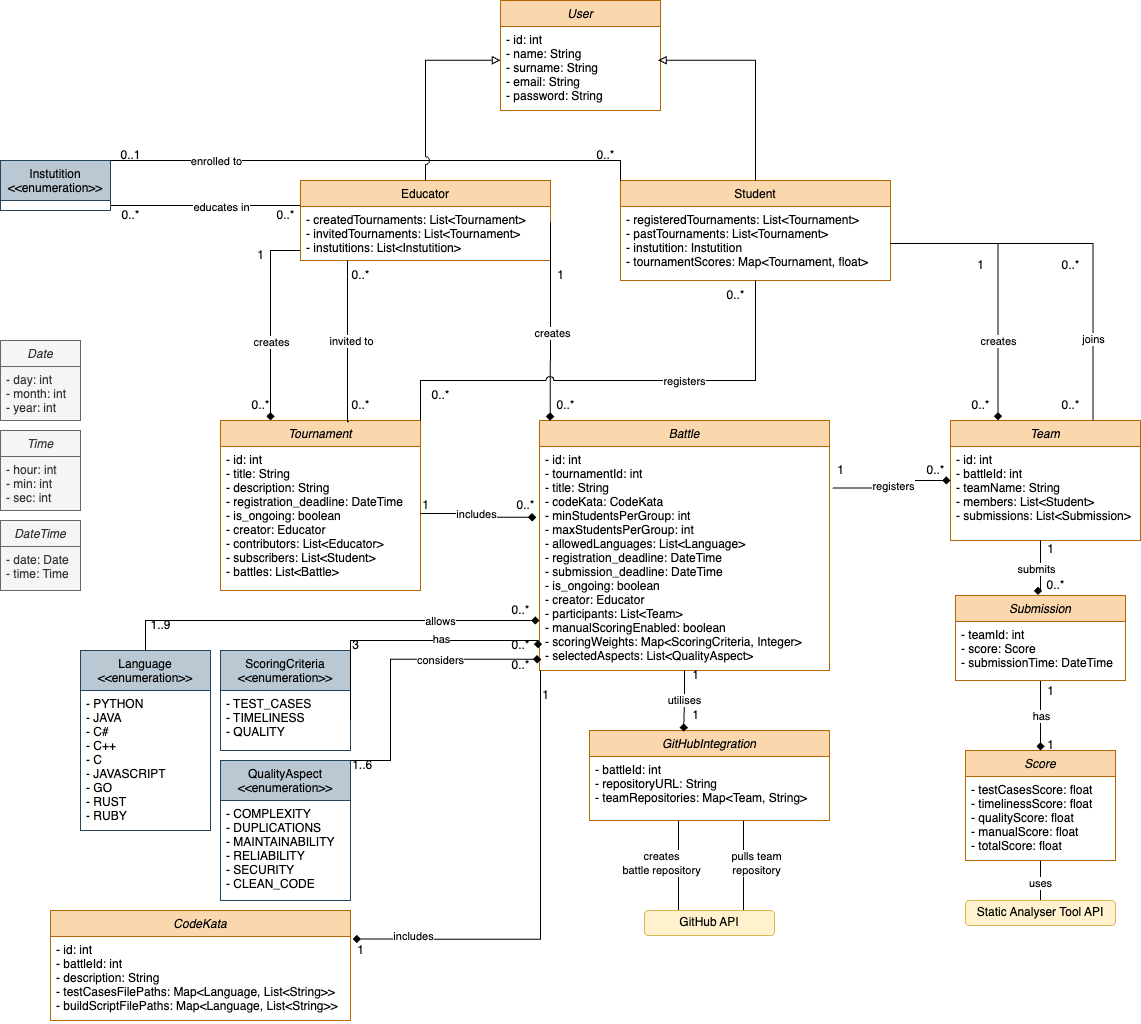
\includegraphics[width=\textwidth,height=\textheight,keepaspectratio]{Images/domainclassdiagramfinal.drawio.png}
    \caption{Domain Class Diagram}
    \label{fig:dcd}
\end{figure}


The descriptions below are the explanations of the important classes that take place in the diagram:
\begin{itemize}
    \item \textbf{User:} Serves as a base for different types of users. It encapsulates common attributes that are shared across students and educators. This class is essential for authentication.

    \item \textbf{Educator:} The objects of this class have the ability to create tournaments and battles. They can also be invited to a tournament by the creator of that tournament. 

    \item \textbf{Students:} The objects of this class have the ability to register for the tournaments, and they can create teams for battles or join teams that they are invited to.

    \item \textbf{Tournament:} Tournaments are a vital part of the project. They are created by educators and they include coding battles for teams of students to engage and solve.

    \item \textbf{Battle:} Battles are created by educators who take part in a tournament. During battle creation, educators set some of the fields of the battle object.

    \begin{itemize}
        \item \textbf{Scoring Criteria:} There exists 3 scoring criteria whose percentages are decided by the educator during battle creation.

        \item \textbf{Language:} There are 9 languages allowed in the system. The educator chooses the allowed languages during battle creation. At least one language must be chosen.

        \item \textbf{Quality Aspect:} There are 6 quality aspects that can be selected by the educator during battle creation time. At least one quality aspect must be chosen.

        \item \textbf{CodeKata:} It is the most important part of the battle. The test cases and the build scripts for each allowed language should be uploaded by the educator to the system. The paths to the files in the file system are stored in the fields.
    \end{itemize}

    \item \textbf{Team:} Teams are created by students, and the teams are able to register for the battles. They have a score for the battle.

    \item \textbf{GitHub Integration:} This class has one object for each battle and it stores the link to the GitHub repository for the battle after creating it by interacting with the GitHub API. It also stores the links to the repositories of the participating teams after they push their code and trigger a function that belongs to this class.

    \item \textbf{Submission}: Submissions are delivered by teams registered to battles. They have submission time and score of the submission.

    \item \textbf{Score:} The score of a team for each criterion is calculated for the battle. This class uses an external Static Analyser Tool to calculate the score of the quality aspect of the code. The timeliness and test case scores are handled internally.
\end{itemize}

\newpage
\subsubsection{Statecharts}
The state charts presented in this section elucidate the operation of the CodeKataBattle (CKB) project, illustrating the state transitions for a code kata battle and a tournament within the platform. Especially for tournaments, a state chart is very crucial to gain a better understanding of the tournament.\newline
\textbf{Tournament}

\begin{figure}[H]
    \centering
    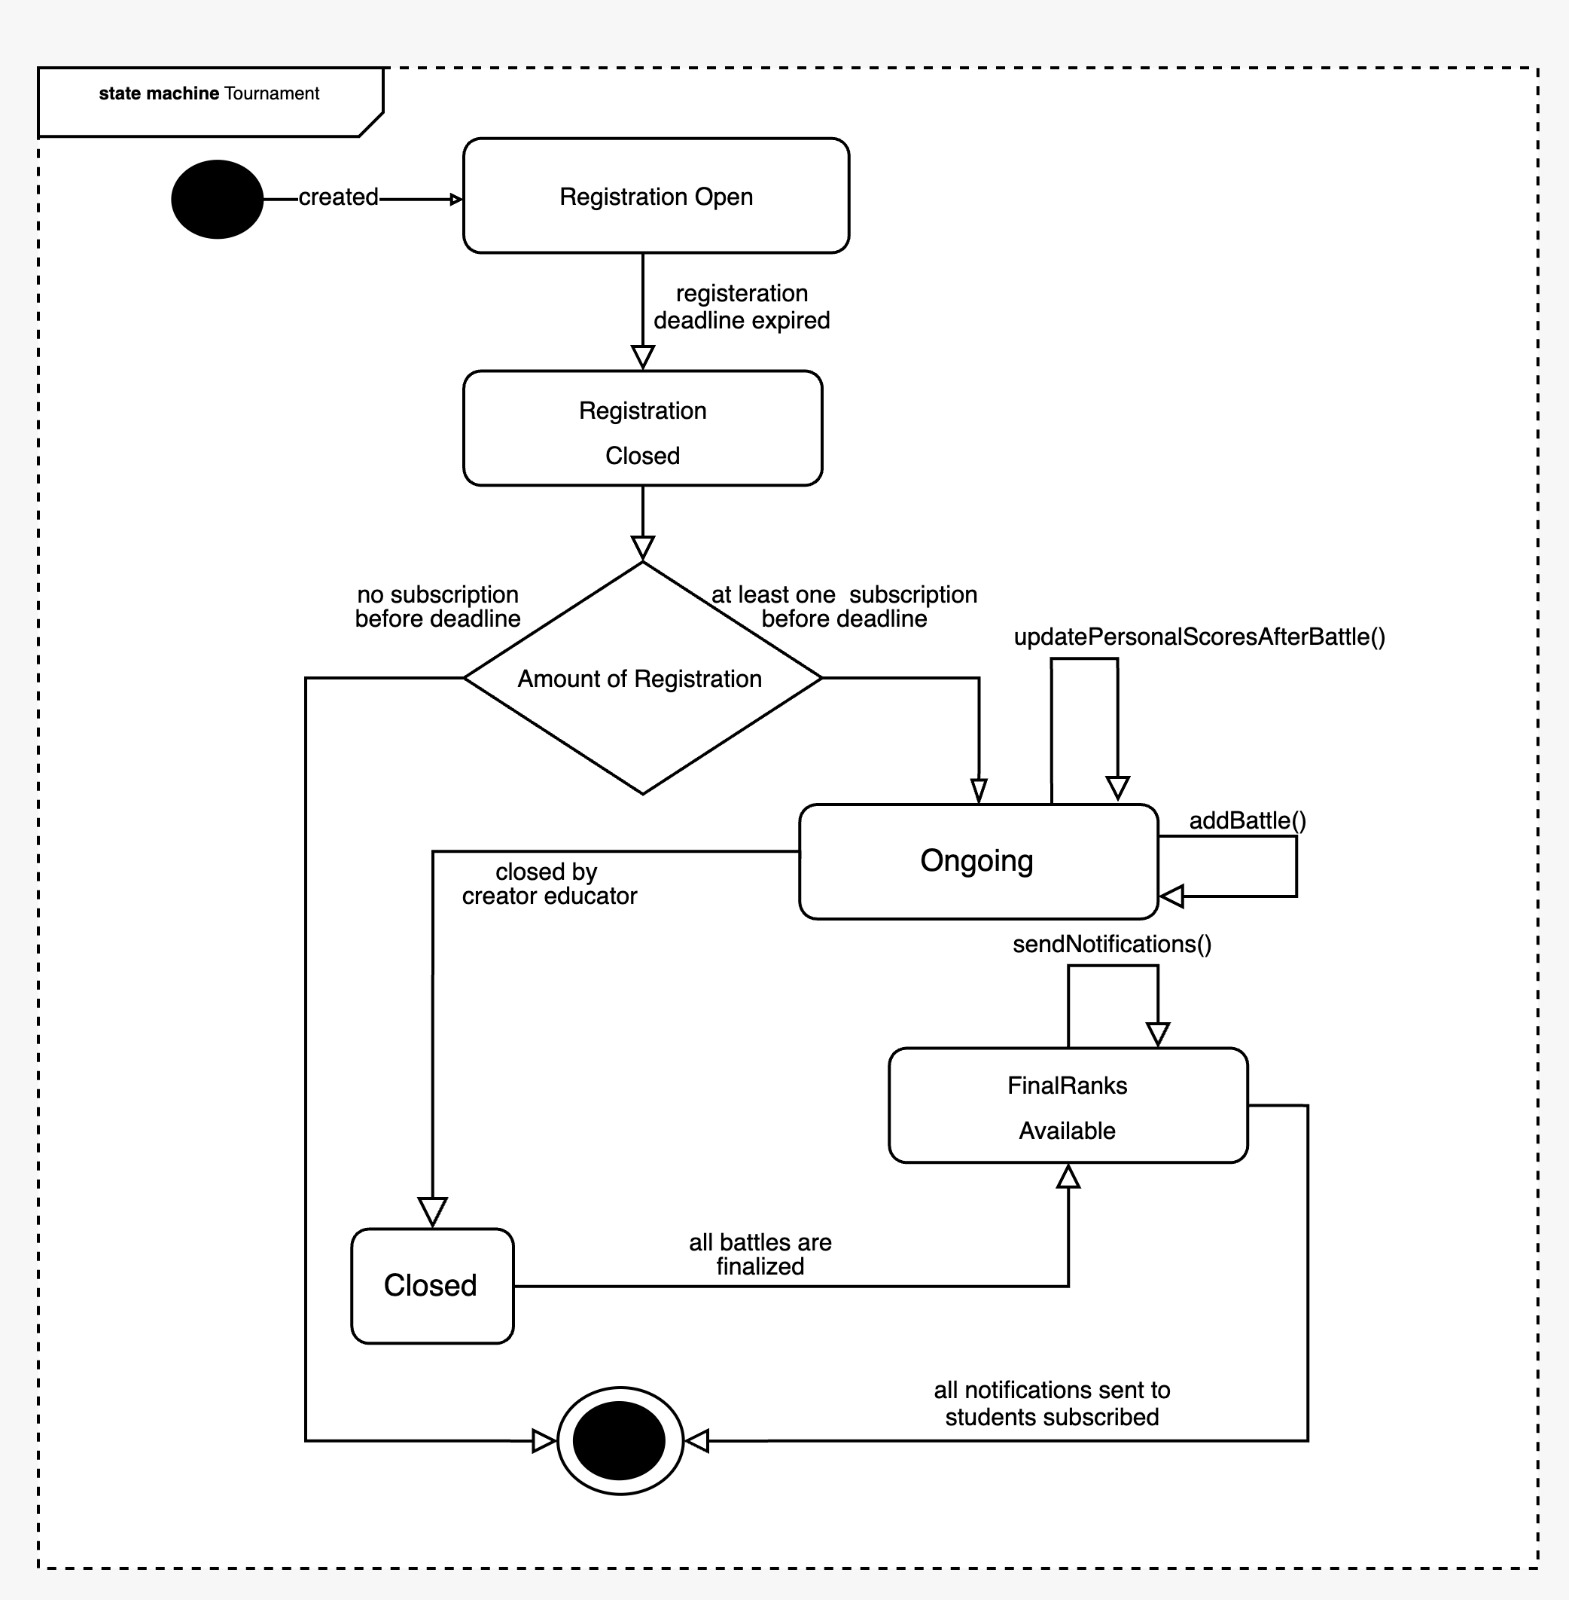
\includegraphics[scale=0.2]{Images/state_diagram/state_diagram_tournament.jpeg}
    \caption{$SC_{1}$ - Tournament}
    \label{fig:sc-t}
\end{figure}

Firstly, the tournament is in the very first state called "Registration Open", which indicates that Tournament is created and registration is open for students and invited educators. Until the registration deadline, they can register. When the deadline expires registration is closed, so the tournament goes into the "Registration Closed" state. In this state, the process controls the amount of registration for the tournament. If there is no registration it goes to "Final" state. Otherwise, the tournament starts with the "Ongoing" state. In this state, throughout the tournament, educators can create battles, and personal scores are updated after every battle. If the creator educator closes the tournament, it goes to the "Closed" state. However, there can be some battles in the consolidation stages and it is mandatory to finalize them to calculate final ranks. After every battle is finalized, the tournament transitions to the "FinalRankAvailable" state in which notifications about final rankings are sent to the students. After finishing this notification process tournament reaches the "Final" state. There won't be any rank changes or notifications hereafter. \newpage
\textbf{Battle}\newline

\begin{figure}[H]
    \centering
    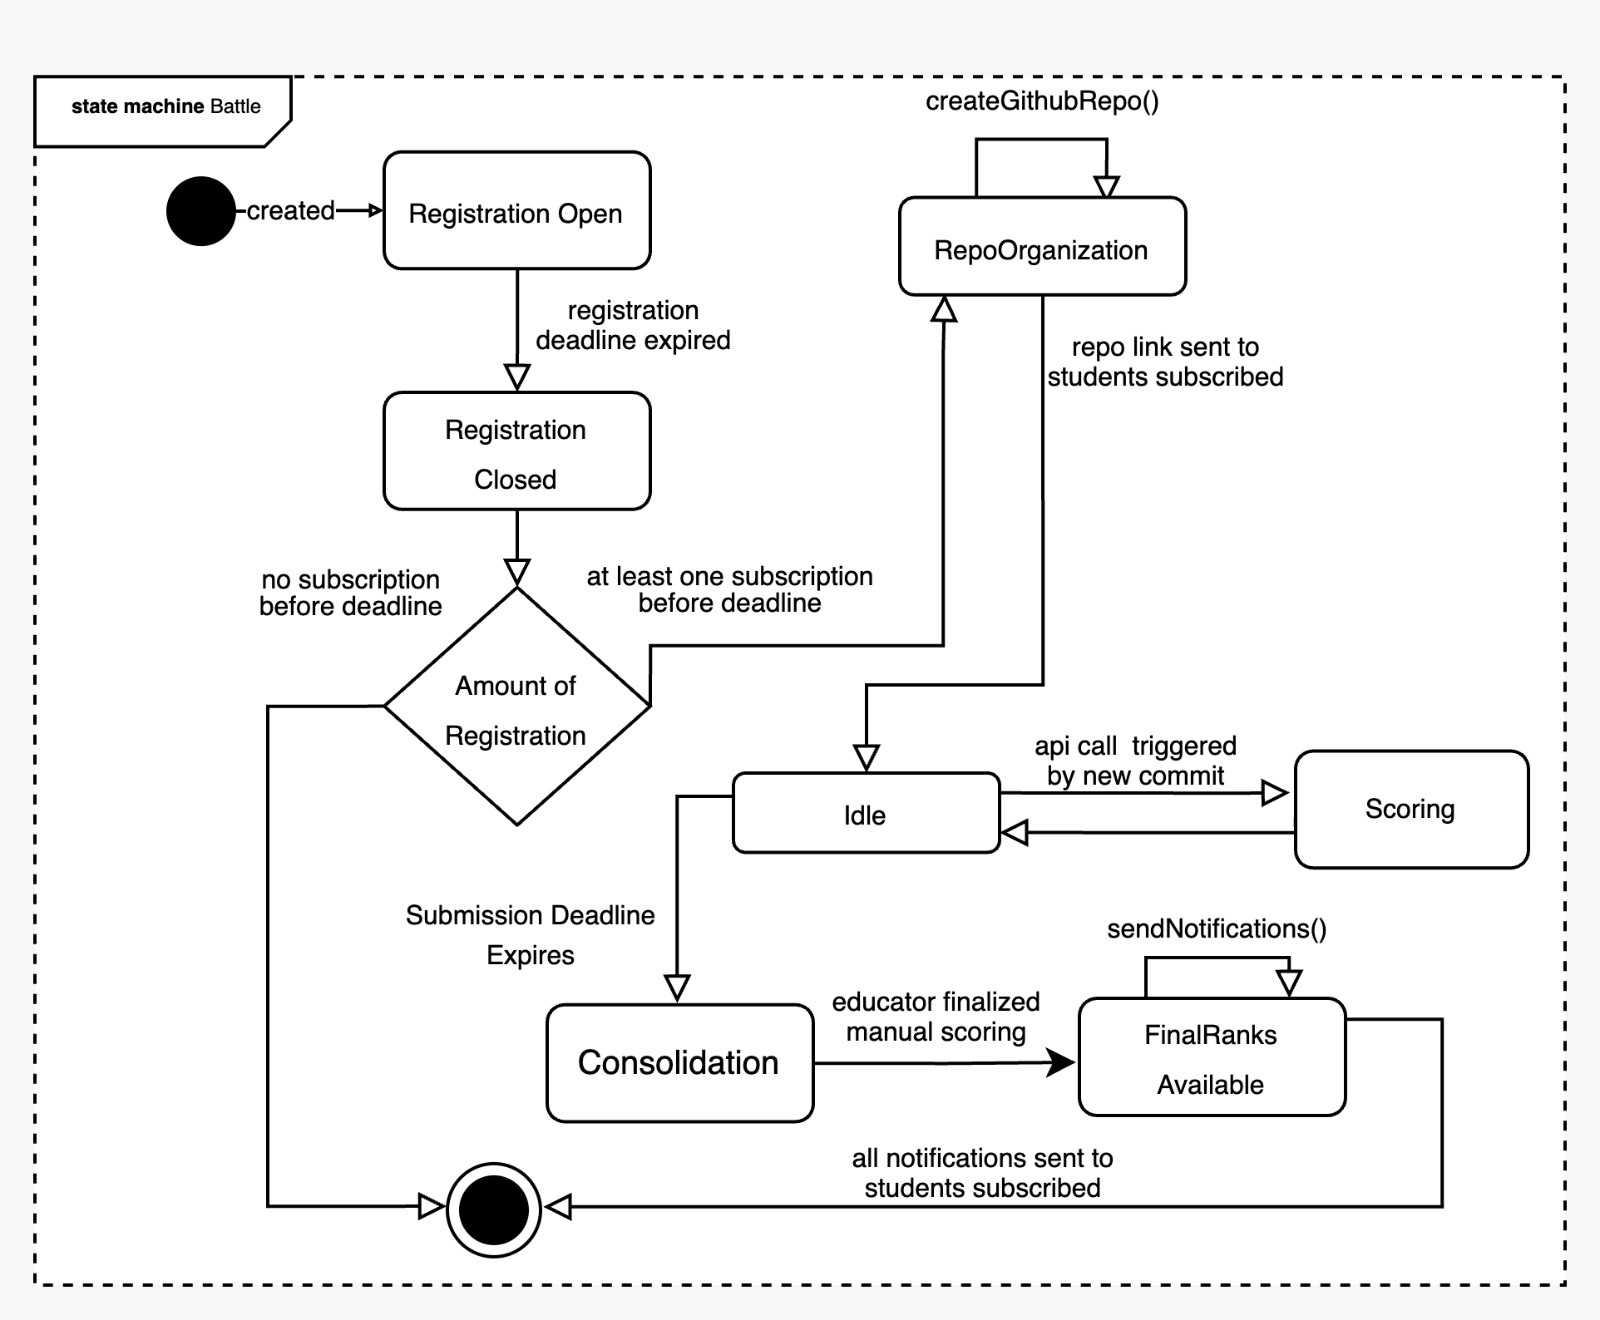
\includegraphics[scale=0.2]{Images/state_diagram/state_diagram_battle.jpeg}
    \caption{$SC_{2}$ - Battle}
    \label{fig:sc-b}
\end{figure}

Firstly tournament is created with the "Registration Open" state. In this state, students can register to battle with teams or individually. When the deadline expires, Battle goes into the "Registration Closed" state. At this time, it is calculated that if there is any registration for battle. If no, it goes to the "Final" state with no registration and any other action. If there are registrations, it goes to a new state called as RepoOrganization in which GitHub repository for the battle is created with proper instructions. Sending the link and instructions triggers the process to go into the "Idle" state. This means that Battle has started and waits for API calls from forked repositories, triggered by a new commit. An API call from repositories of competitor leads to scoring phase. Until the submission deadline, battle switches between Scoring and Idle states.Eventually, it returns to the "Idle" state. Until the submission deadline, students' commit can change their scores. When the deadline expires, Battle goes into the "Consolidation Stage" state in which educators can change rankings via manual scorings. When they are finalized, Battle is closed, indicating as state "FinalRanksAvailable". Immediately, the notification sending process starts. After all notifications are sent, Battle goes into the Final state.
\newpage
\textbf{Submission}\newline

\begin{figure}[H]
    \centering
    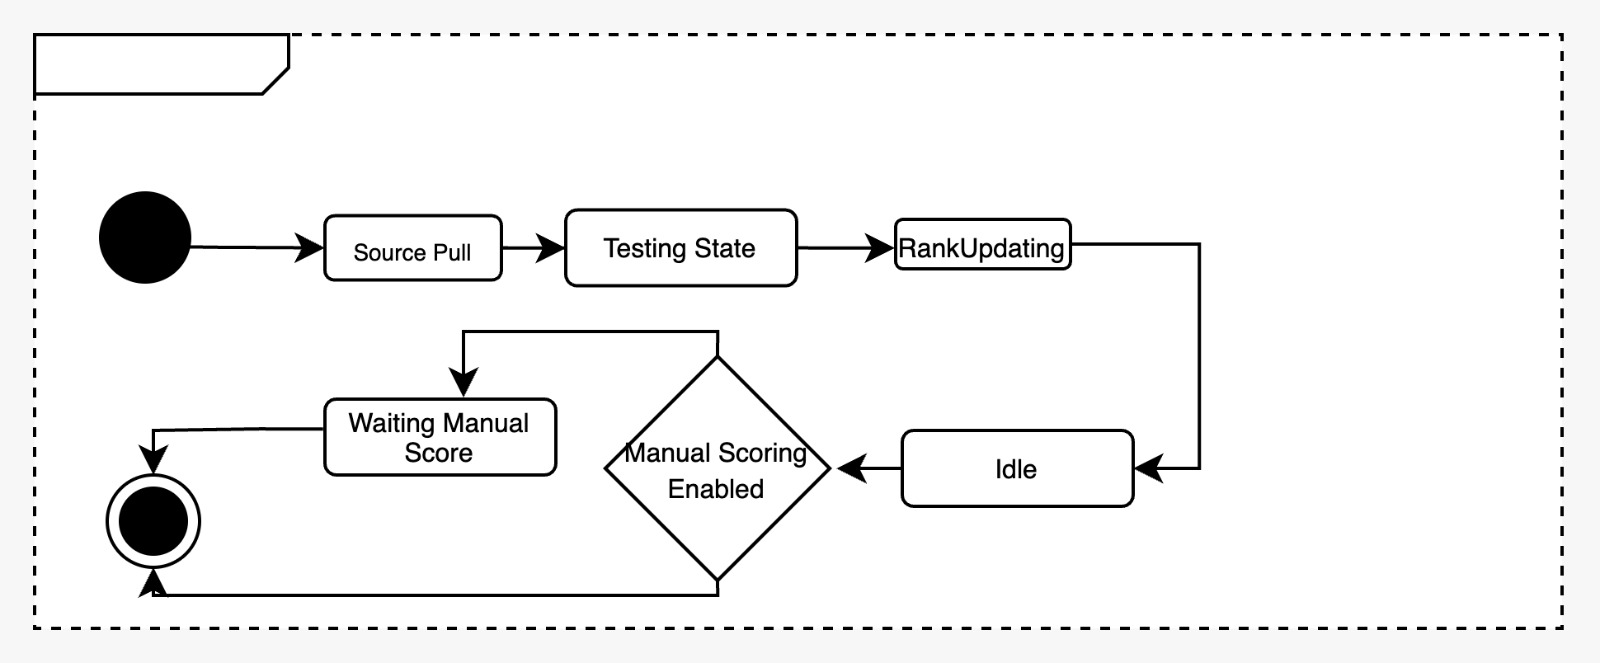
\includegraphics[scale=0.2]{Images/state_diagram/state_diagram_submission.jpeg}
    \caption{$SC_{3}$ - Submission}
    \label{fig:sc-s}
\end{figure}


Firstly, Submission goes into source pulling and initialization phases. After Testing and Rank Updating, which are sequential phases, submission become idle until the submission deadline. In there, either it goes into consolidation stage for manual scoring or immediately finalized. rankings are updated.
\newpage

\subsubsection{Activity Diagrams}
\textbf{Register Battle}
\begin{figure}[H]
    \centering
    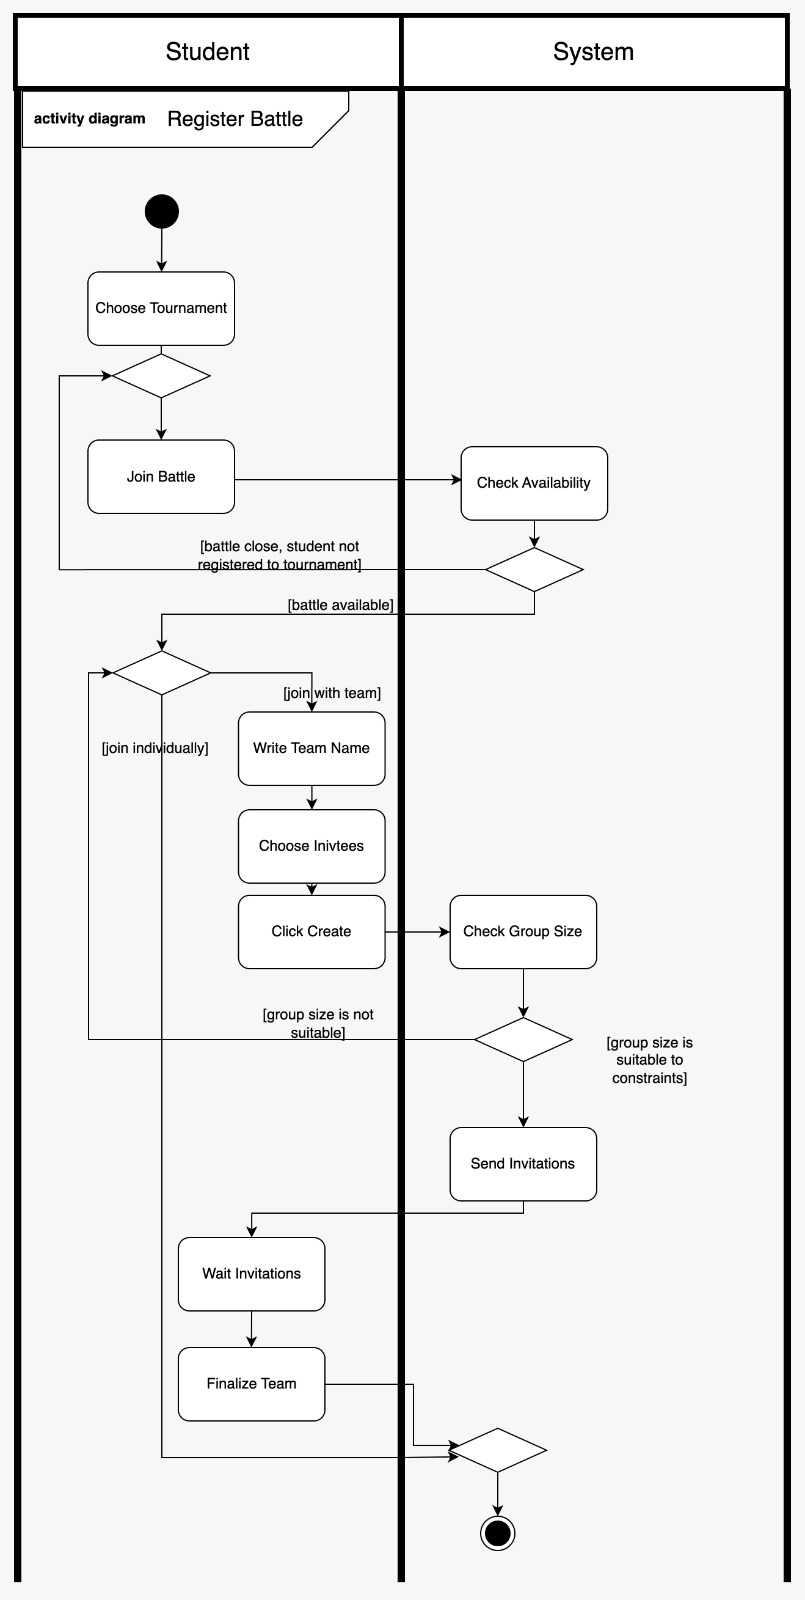
\includegraphics[scale=0.27]{Images/activity_diagram/activity_diagram_register_battle.jpeg}
    \caption{$AC_{1}$ - Register Battle}
\end{figure}


\newpage
\textbf{Create Battle}
\begin{figure}[H]
    \centering
    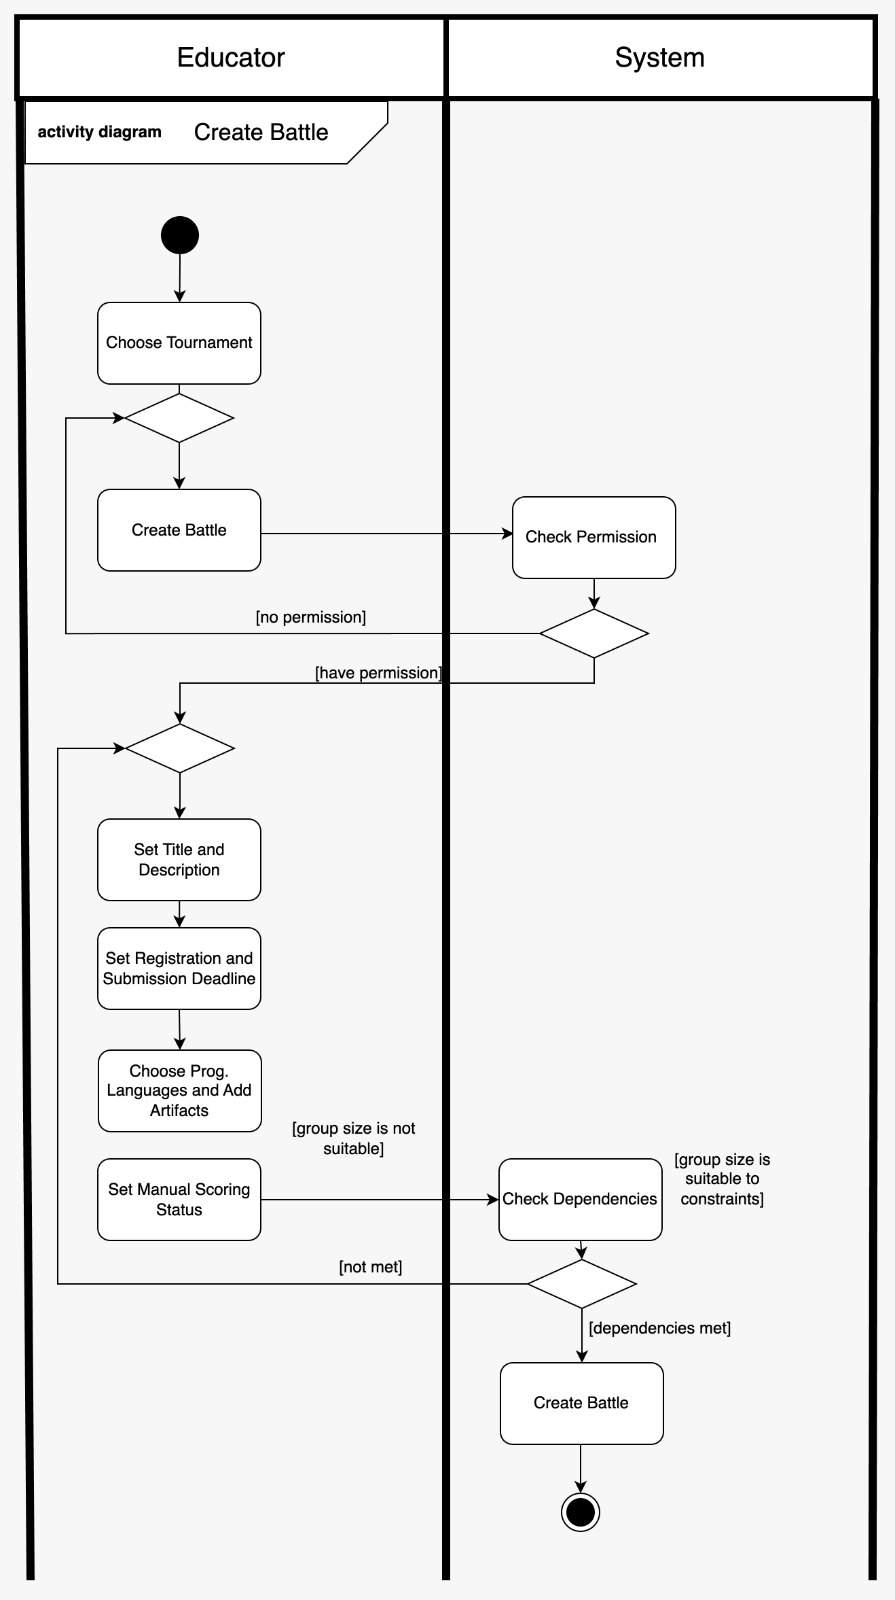
\includegraphics[scale=0.327]{Images/activity_diagram/activity_diagram_create_battle.jpeg}
    \caption{$AC_{2}$ - Create Battle}
\end{figure}

\newpage
\textbf{Submission}
\begin{figure}[H]
    \centering
    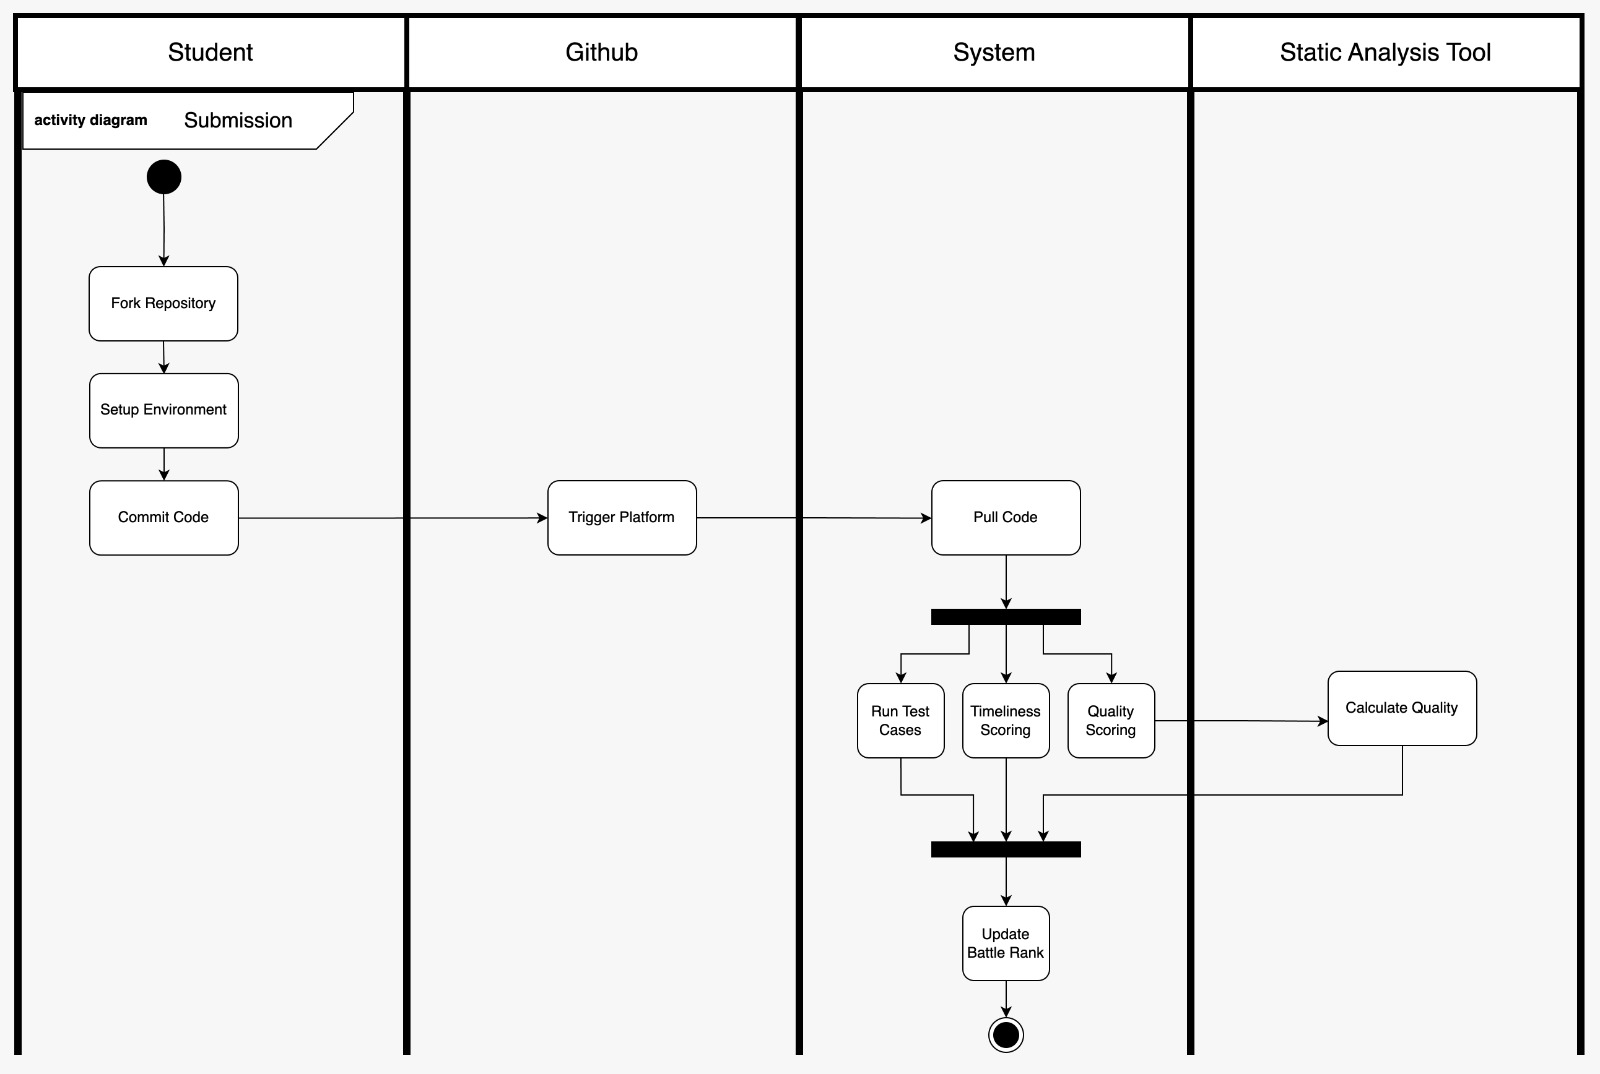
\includegraphics[scale=0.27]{Images/activity_diagram/activity_diagram_submission.jpeg}
    \caption{$AC_{3}$ - Submission}
\end{figure}

\newpage
\subsection{Product Functions}

The major functions of the project will be organised according to the user types. We will have three sections, first for the common function both regarding the educators and the students. The second and the third will be specific to each user type respectively.

\subsubsection{Common Functions}

\begin{itemize}
    \item \textbf{Account Registration:} Both students and educators can be registered to the platform. During registration, the user indicated which type of user they are along with their credentials.

    \item \textbf{Viewing Leaderboards and Rankings:} Both user types can view leaderboards that display rankings of participants based on performance in battles and overall tournament standings.
\end{itemize}

\subsubsection{Educator Functions}
\begin{itemize}
    \item \textbf{Creating a Tournament:} Educators can create and configure tournaments, setting specific parameters such as time constraints. In these tournaments, multiple battles can take place.

    \item \textbf{Creating a Battle:} Educators can create and configure coding battles in the tournament that they have created or they have been permitted by their fellow educators. During battle creation, specific parameters such as coding languages, and team sizes are set by the educator. On top of that, the description of the battle and the test file including test cases, automated build scripts or manual evaluation choice should be provided.

    \item \textbf{Giving Permission to Other Educators:} This function can be utilised both in the creation of a tournament and during the management of a tournament. Educators are able to permit fellow educators to create battles in the tournaments that they have created.

    \item \textbf{Scoring:} This function is vital since it is used to compute the points of the students' submissions in the battles. The output of this method determines the ranking of the students. Both automated and manual scoring reply to this function call.
    
\end{itemize}

\subsubsection{Student Functions}
\begin{itemize}
    \item \textbf{Join a Tournament:} Students can join tournaments that the educators are created. When they join a tournament, they will be able to take part battles in it.

    \item \textbf{Join a Battle:} Students can join battles which is a part of the tournament they already joined. When joining the battle, students can send requests to other students to form a team if they want or need to.

    \item \textbf{Send Request for Teaming:} This function can be called during students join the battle. Students send requests to other students using their usernames, and if they accept the invitation, they are now a part of the team for the battle they are joining.

    \item \textbf{Submit Solution:} Students submit their solutions for each code battle. After submission successfully completed, the scoring function is called.
\end{itemize}





\newpage
\subsection{User Characteristics}

\subsubsection{Educators}

\begin{enumerate}[A.]
    \item \textbf{Profile}

        \begin{itemize}
            \item Typically instructors, professors, or teachers in computer science or related fields, with varying levels of experience in coding and software development education.
        \end{itemize}

    \item \textbf{Needs}

        \begin{itemize}
            \item Tools for creating, managing, and monitoring coding challenges and tournaments.
            \item Flexibility in setting parameters for battles, including team sizes, deadlines, and testing criteria.
            \item Ability to assess student work both automatically or manually.
            \item Resources to track student progress and engagement in coding exercises.
        \end{itemize}

    \item \textbf{Interactions}

        \begin{itemize}
            \item Making students engage with battles for educational purposes.
            \item Collaboration with other educators within or across institutions.
        \end{itemize}
    
\end{enumerate}

\subsubsection{Students}

\begin{enumerate}[A.]
    \item \textbf{Profile}

        \begin{itemize}
            \item Individuals enrolled in computer science and similar courses or those seeking to enhance their coding skills, ranging from beginners to advanced levels.
        \end{itemize}

    \item \textbf{Needs}

        \begin{itemize}
            \item Access to a variety of coding challenges that help to improve the student's skills.
            \item Tools for collaborative coding and team formation.
            \item Real-time feedback on code submissions for iterative learning.
            \item Opportunities to apply theoretical knowledge in practical scenarios.
        \end{itemize}

    \item \textbf{Interactions}

        \begin{itemize}
            \item Active participation in coding battles and tournaments.
            \item Collaboration with peers for team-based challenges.
            \item Utilisation of platform resources for self-directed learning and improvement.
        \end{itemize}
    
\end{enumerate}


\newpage
\subsection{Assumptions, Dependencies, and Constraints}

\subsubsection{Domain Assumptions}

\begin{enumerate}
    \item Educators and students have basic proficiency in using web-based platforms and are familiar with basic operations such as account creation, logging in, and navigating through a digital interface.

    \item Educators have the necessary skills to create and manage coding challenges, including the ability to correctly write problem descriptions, test cases, and understand code quality metrics.

    \item The coding problems and challenges provided by educators are free from errors and ambiguities.

    \item Students have at least foundational knowledge in programming and can understand and respond to coding challenges.

    \item Students' submissions to the platform are their original work.

    \item The users have access to reliable internet connectivity and devices capable of supporting the web-based CKB platform.

    \item Students have familiarity with GitHub operations such as forking a repository, setting up GitHub Actions, and committing and pushing their codes.

    \item The automated testing and scoring systems within the CKB platform are trusted by users to fairly and accurately assess coding submissions. Similarly, educators are trusted in the case of manual evaluation of submissions.

\end{enumerate}

\subsubsection{Dependencies}

\begin{itemize}
    \item \textbf{GitHub Services:} The system's functionality for code submission and automated workflow relies on the availability and reliability of GitHub services.

    \item \textbf{Static Analyser Tool:} The system's functionality for code evaluation on quality aspects relies on the availability of an external API that provides Static Analysis.

    \item \textbf{Internet Connectivity:} Access to the internet is essential for both users.

    \item \textbf{Web Browser Compatibility:} The platform's user interface and features depend on their compatibility with various web browsers, ensuring all users can access and use the platform effectively.

    \item \textbf{Hosting Services:} Dependence on reliable hosting services (like cloud-based servers) for hosting the web application, database, and related services.

    \item \textbf{Notification Service:} The platform depends on an external notification service to send timely alerts and updates to students and educators.

    \item \textbf{Email Verification Service:} The platform relies on an external email service provider to send verification codes to users during the account registration process.

    
\end{itemize}


\subsubsection{Constraints}

\begin{itemize}
    \item \textbf{Technological Constraints:} Compatibility requirements with various web browsers and devices may limit certain design or feature implementations.

    \item \textbf{Resource Constraints:} Hosting and operational costs may limit the extent of scalability and redundancy features of the platform.

    \item \textbf{Security and Privacy Constraints:} The system must adhere to strict data protection and privacy regulations, such as GDPR, which may limit certain data collection and processing activities.

    \item \textbf{Legal and Compliance Constraints:} Compliance with intellectual property laws, particularly in the use and distribution of coding challenges and educational content, i.e. the rights of the contents are reserved.
\end{itemize}

%------------------------------------------------------------------------------------------------------------------------------------------------
\clearpage
{\color{Blue}{\section{Specific Requirements}}}
\label{sect:requirements}
\subsection{External Interface Requirements}

\subsubsection{User Interfaces}


In this section, we present user interfaces for Students and Educators. We created a detailed user interface design to inform the reader from a broader perspective. 
\begin{center}
    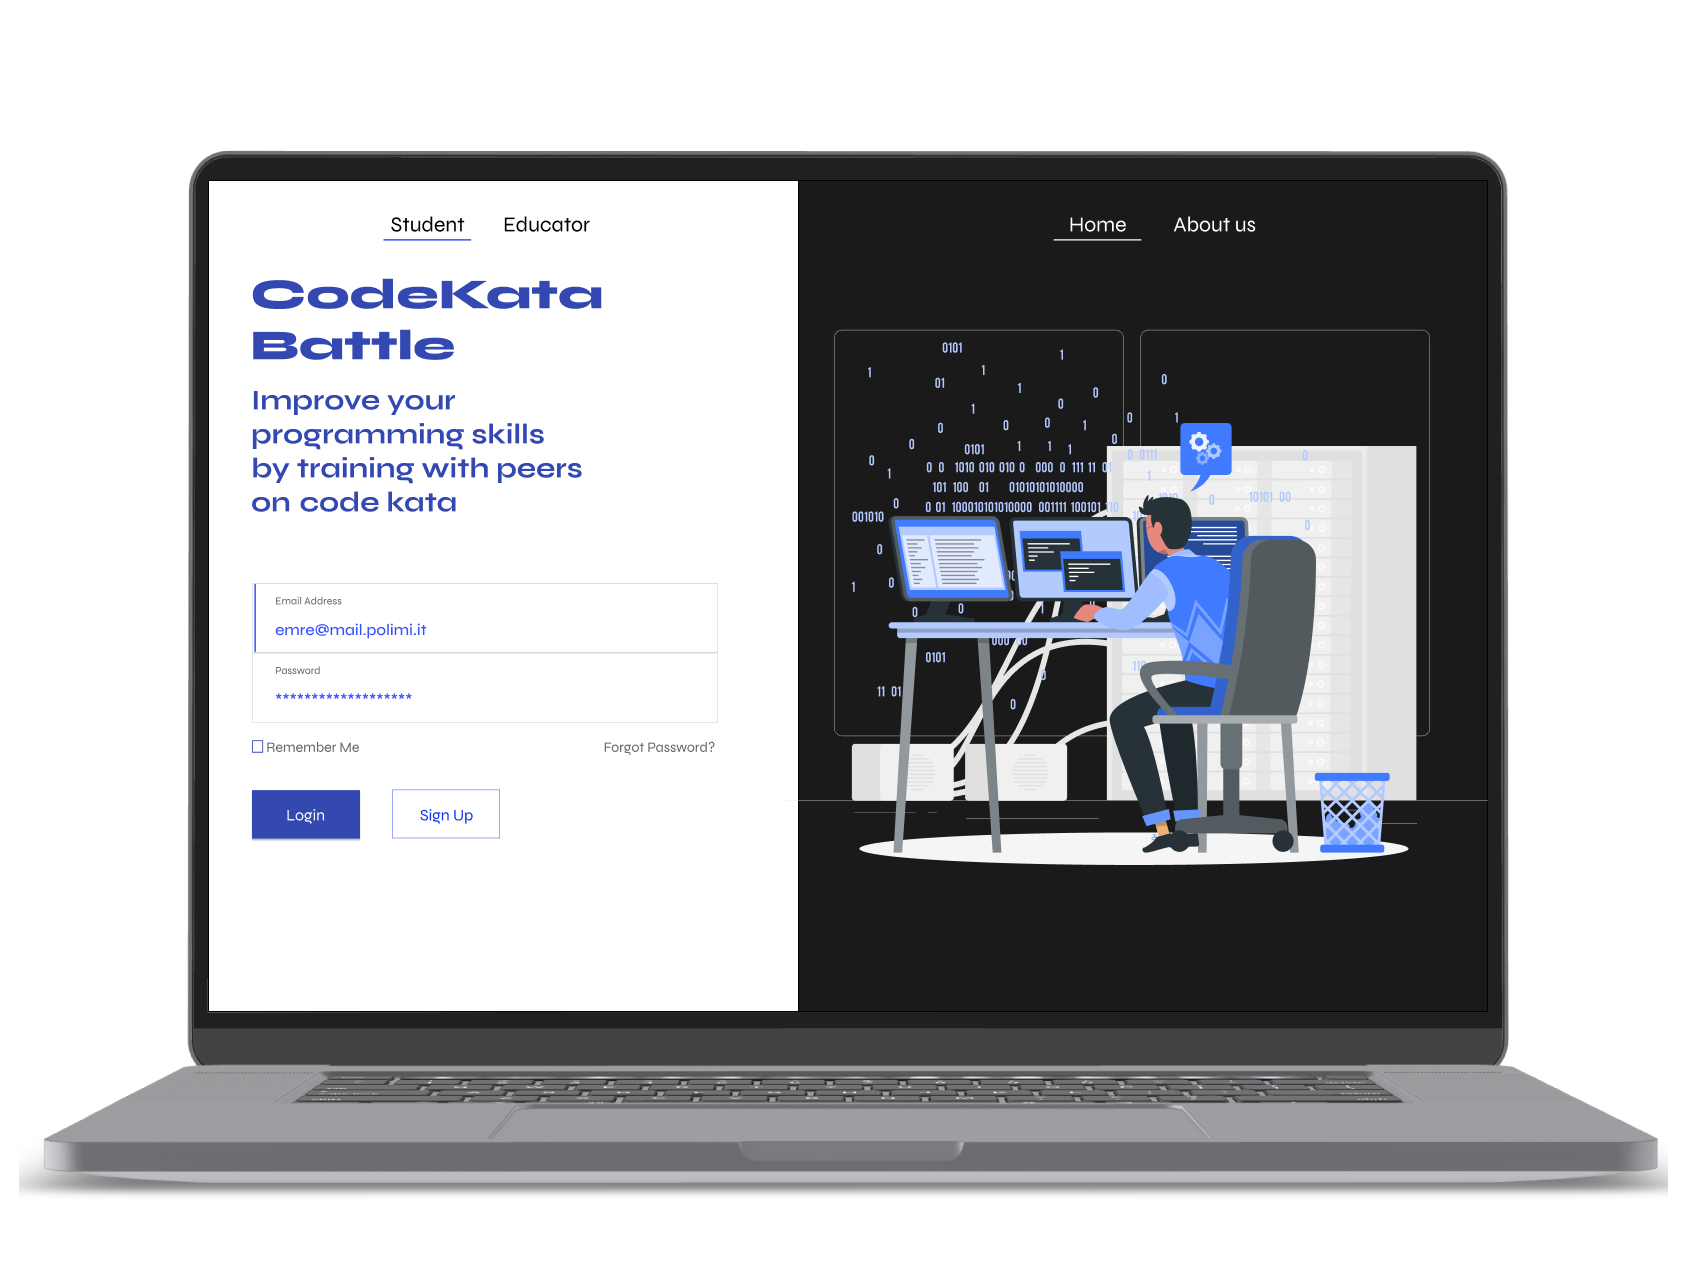
\includegraphics[scale=0.13]{Images/ui-ux/login-signup/student_login.png}
    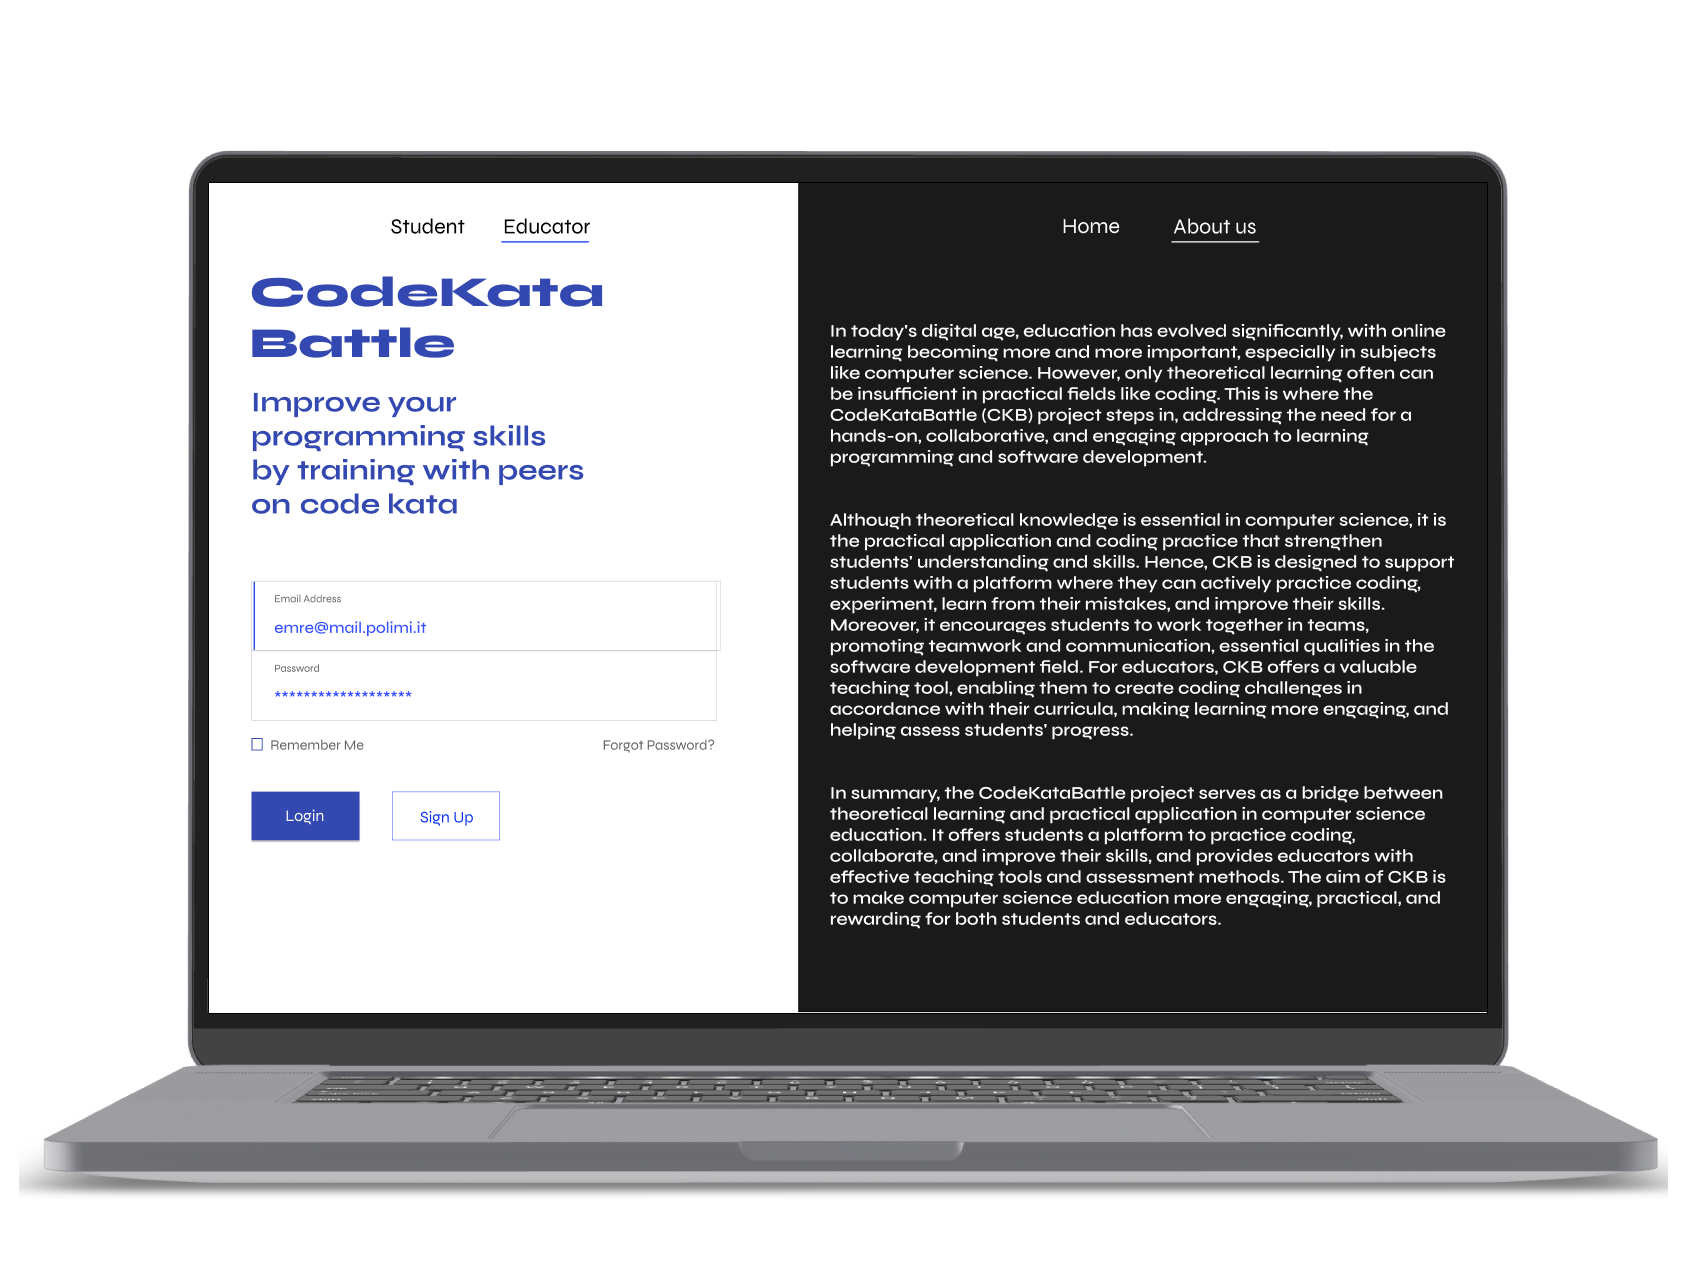
\includegraphics[scale=0.13]{Images/ui-ux/login-signup/educator_login.png}
\end{center}
    \begin{center}
        (a) Login Screens
    \end{center}
\begin{center}
    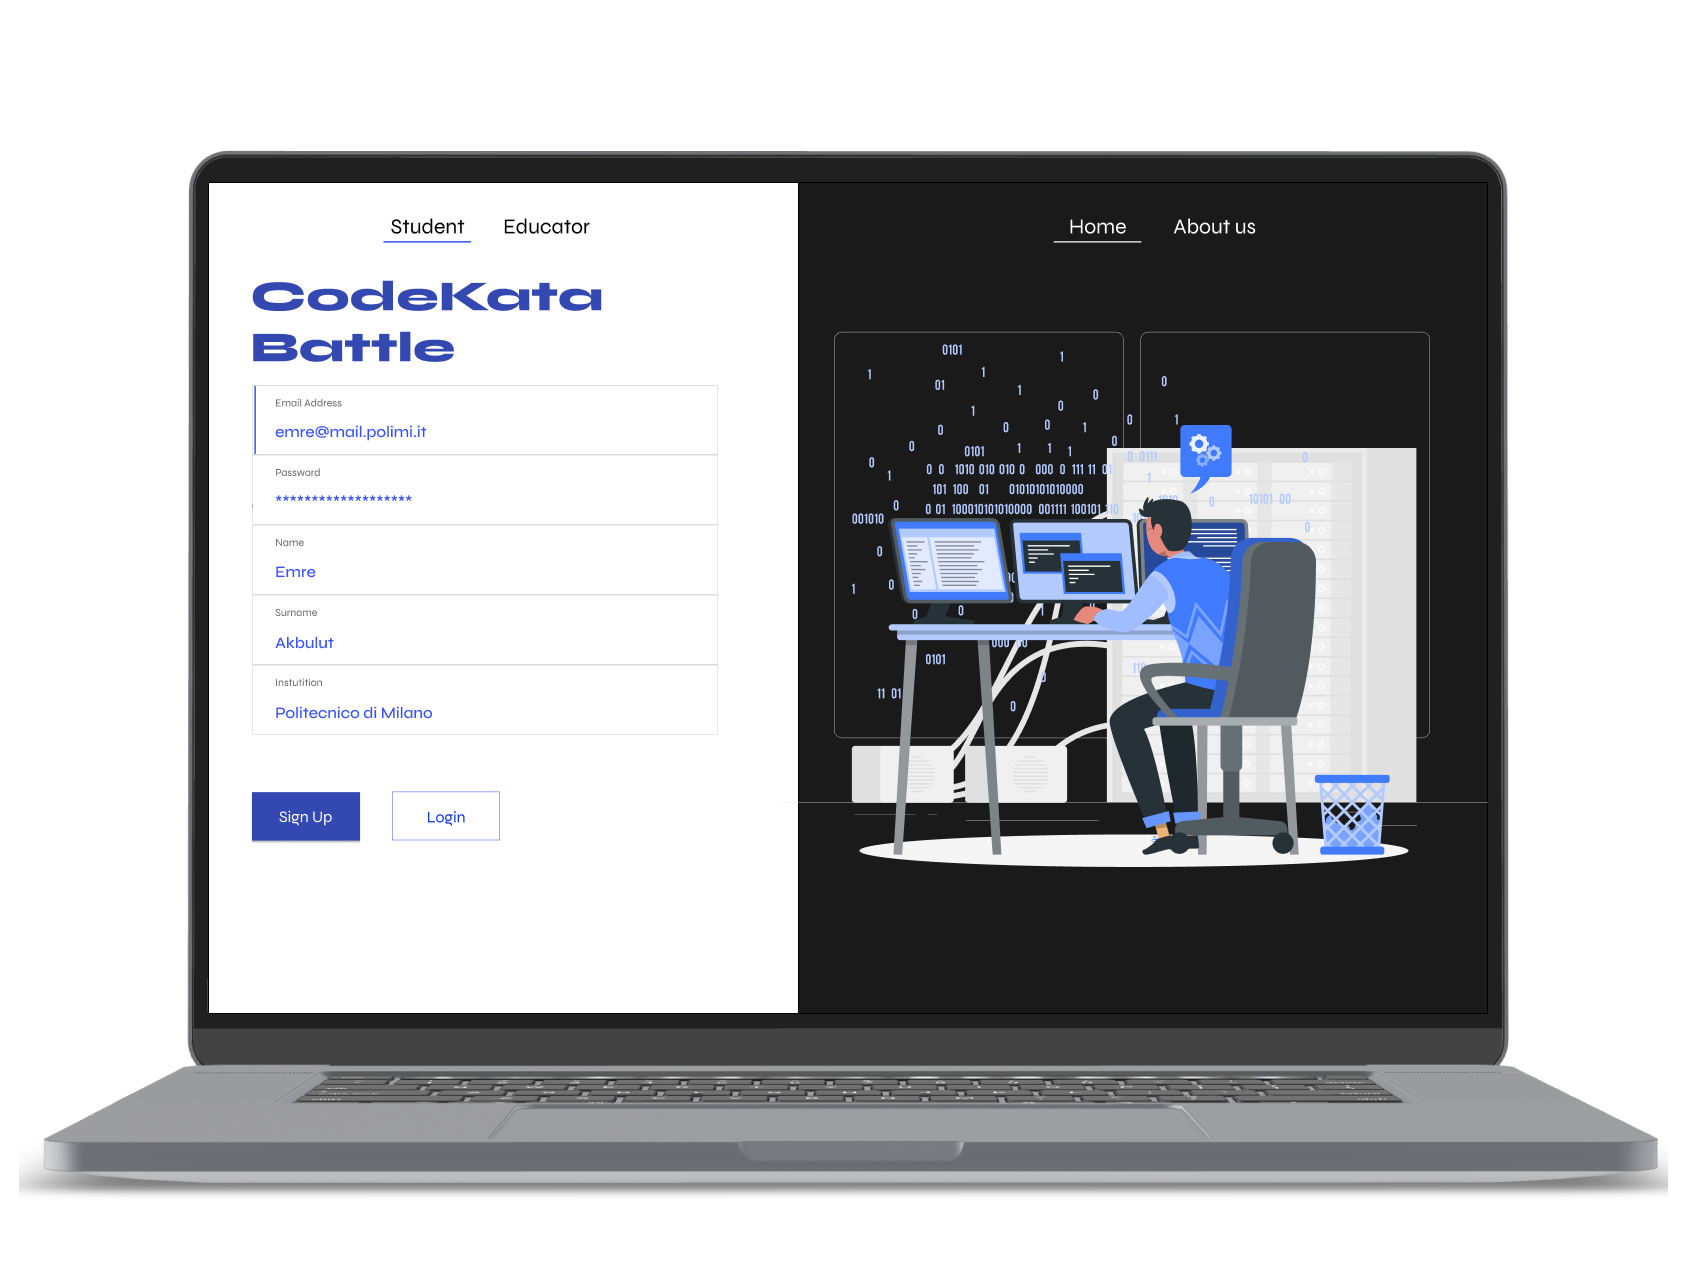
\includegraphics[scale=0.13]{Images/ui-ux/login-signup/student_signup.png}
    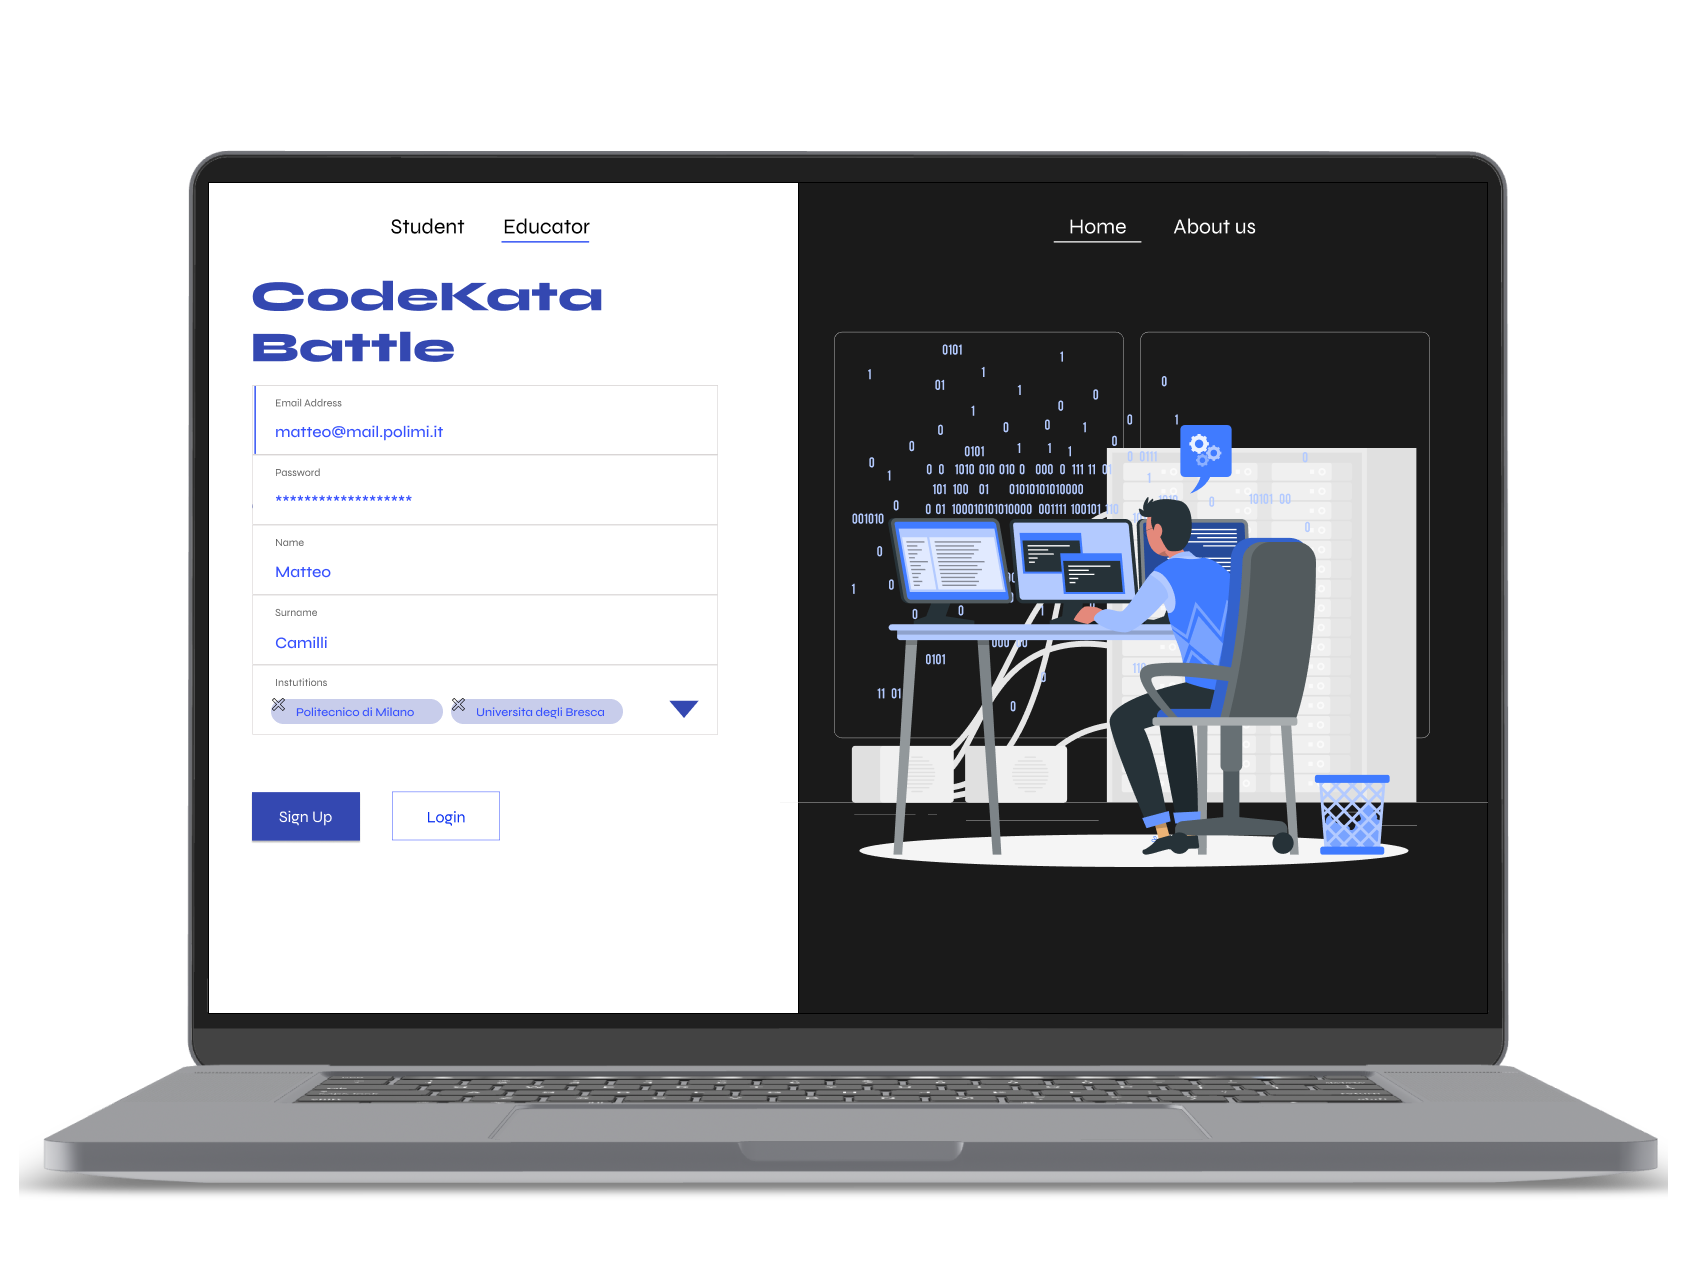
\includegraphics[scale=0.13]{Images/ui-ux/login-signup/educator_signup.png}
    (b) Sign up Screens
\end{center}
\newpage
\begin{center}
    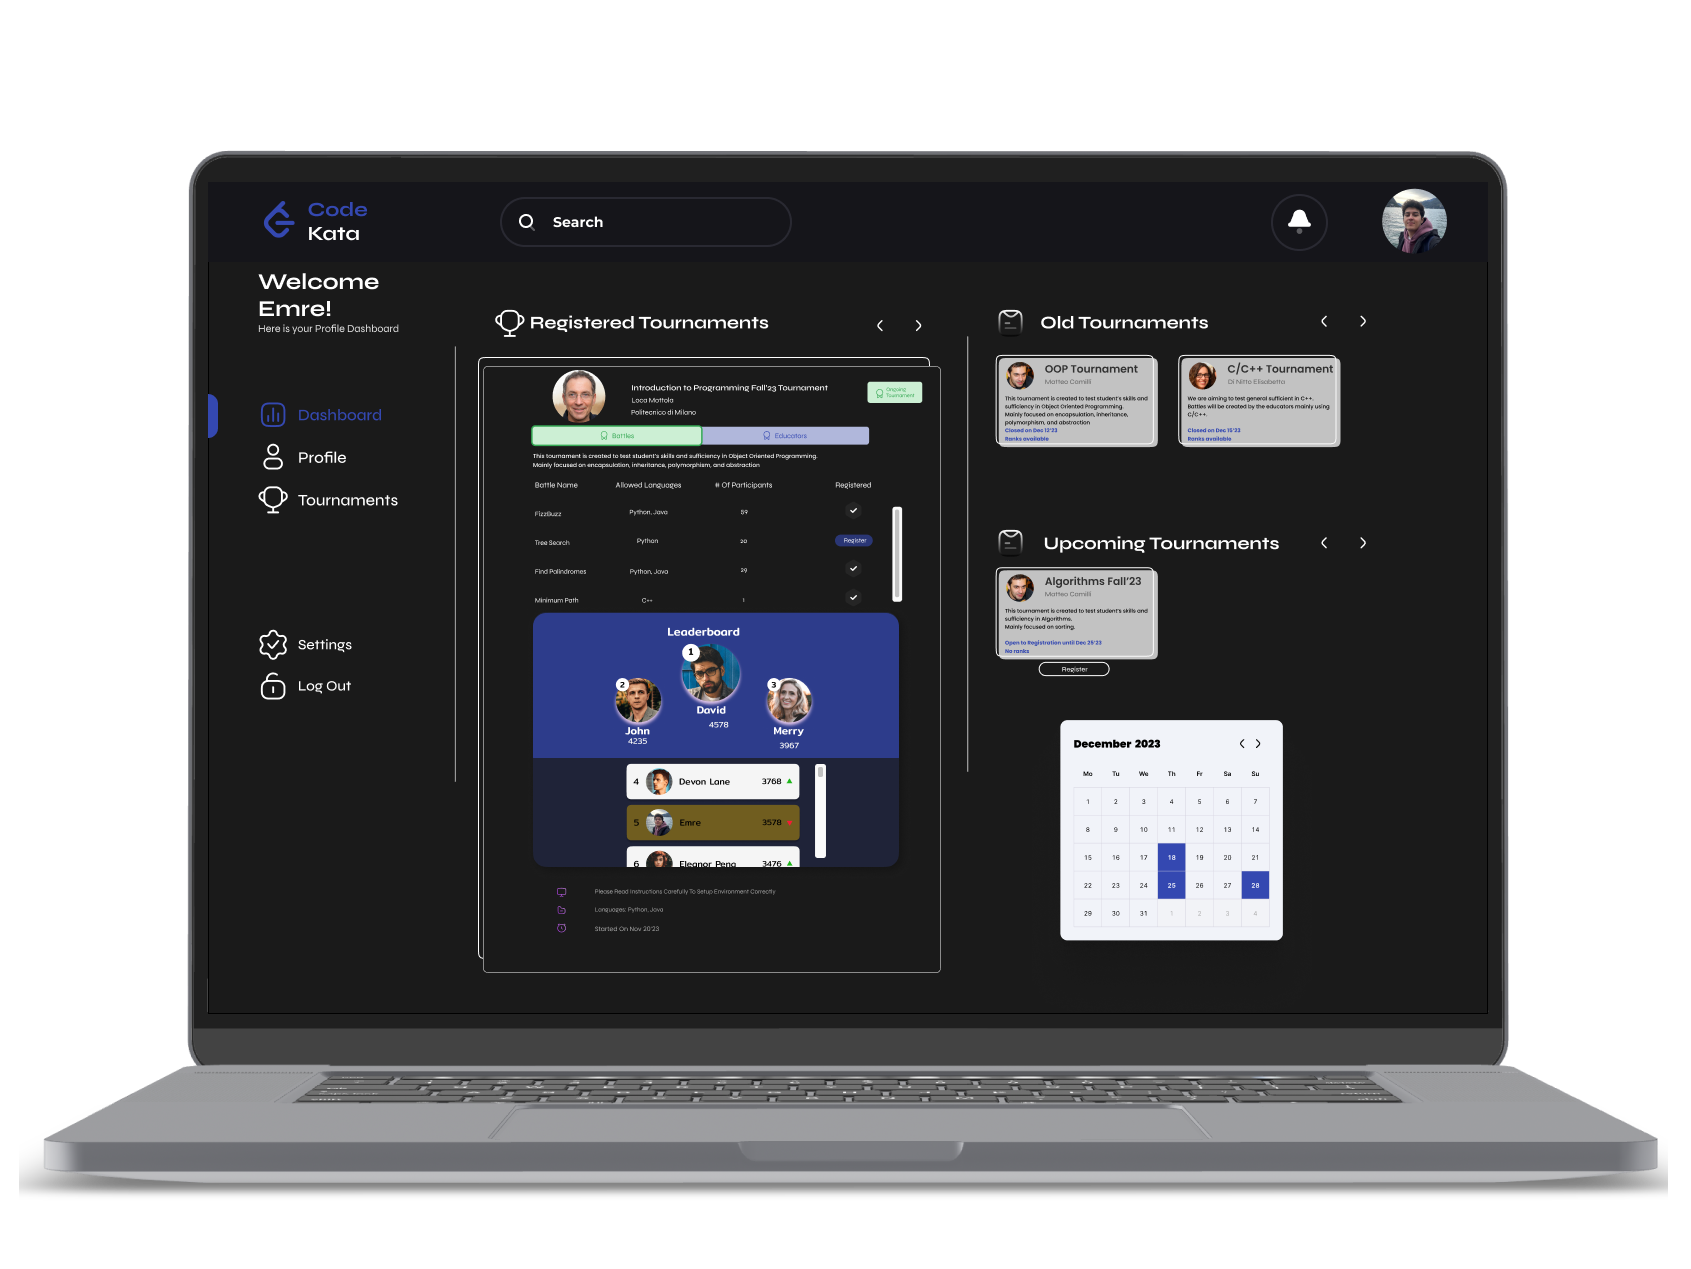
\includegraphics[scale=0.13]{Images/ui-ux/student_dashboard/student_dashboard_1.png}
    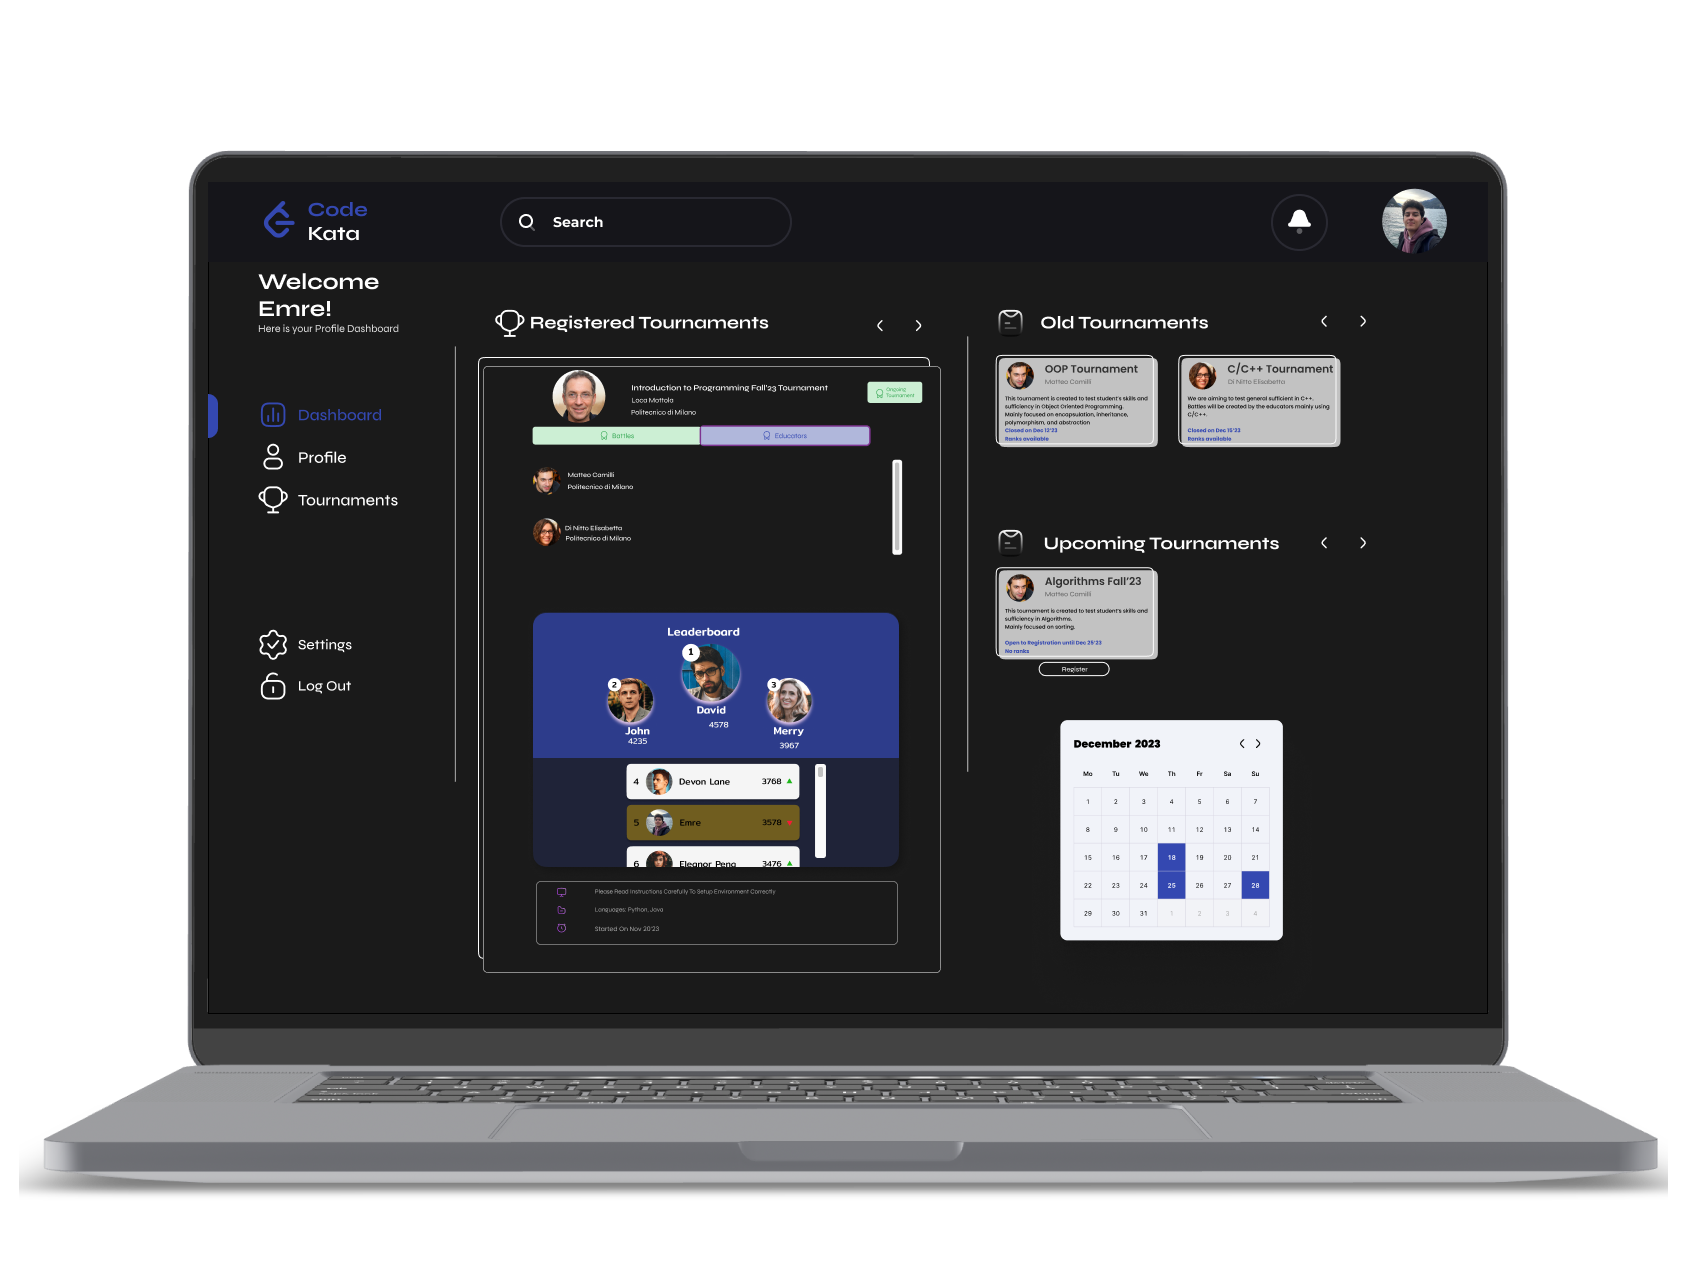
\includegraphics[scale=0.13]{Images/ui-ux/student_dashboard/student_dashboard_2.png}
            (c) Student Dashboard
\end{center}
\begin{center}
    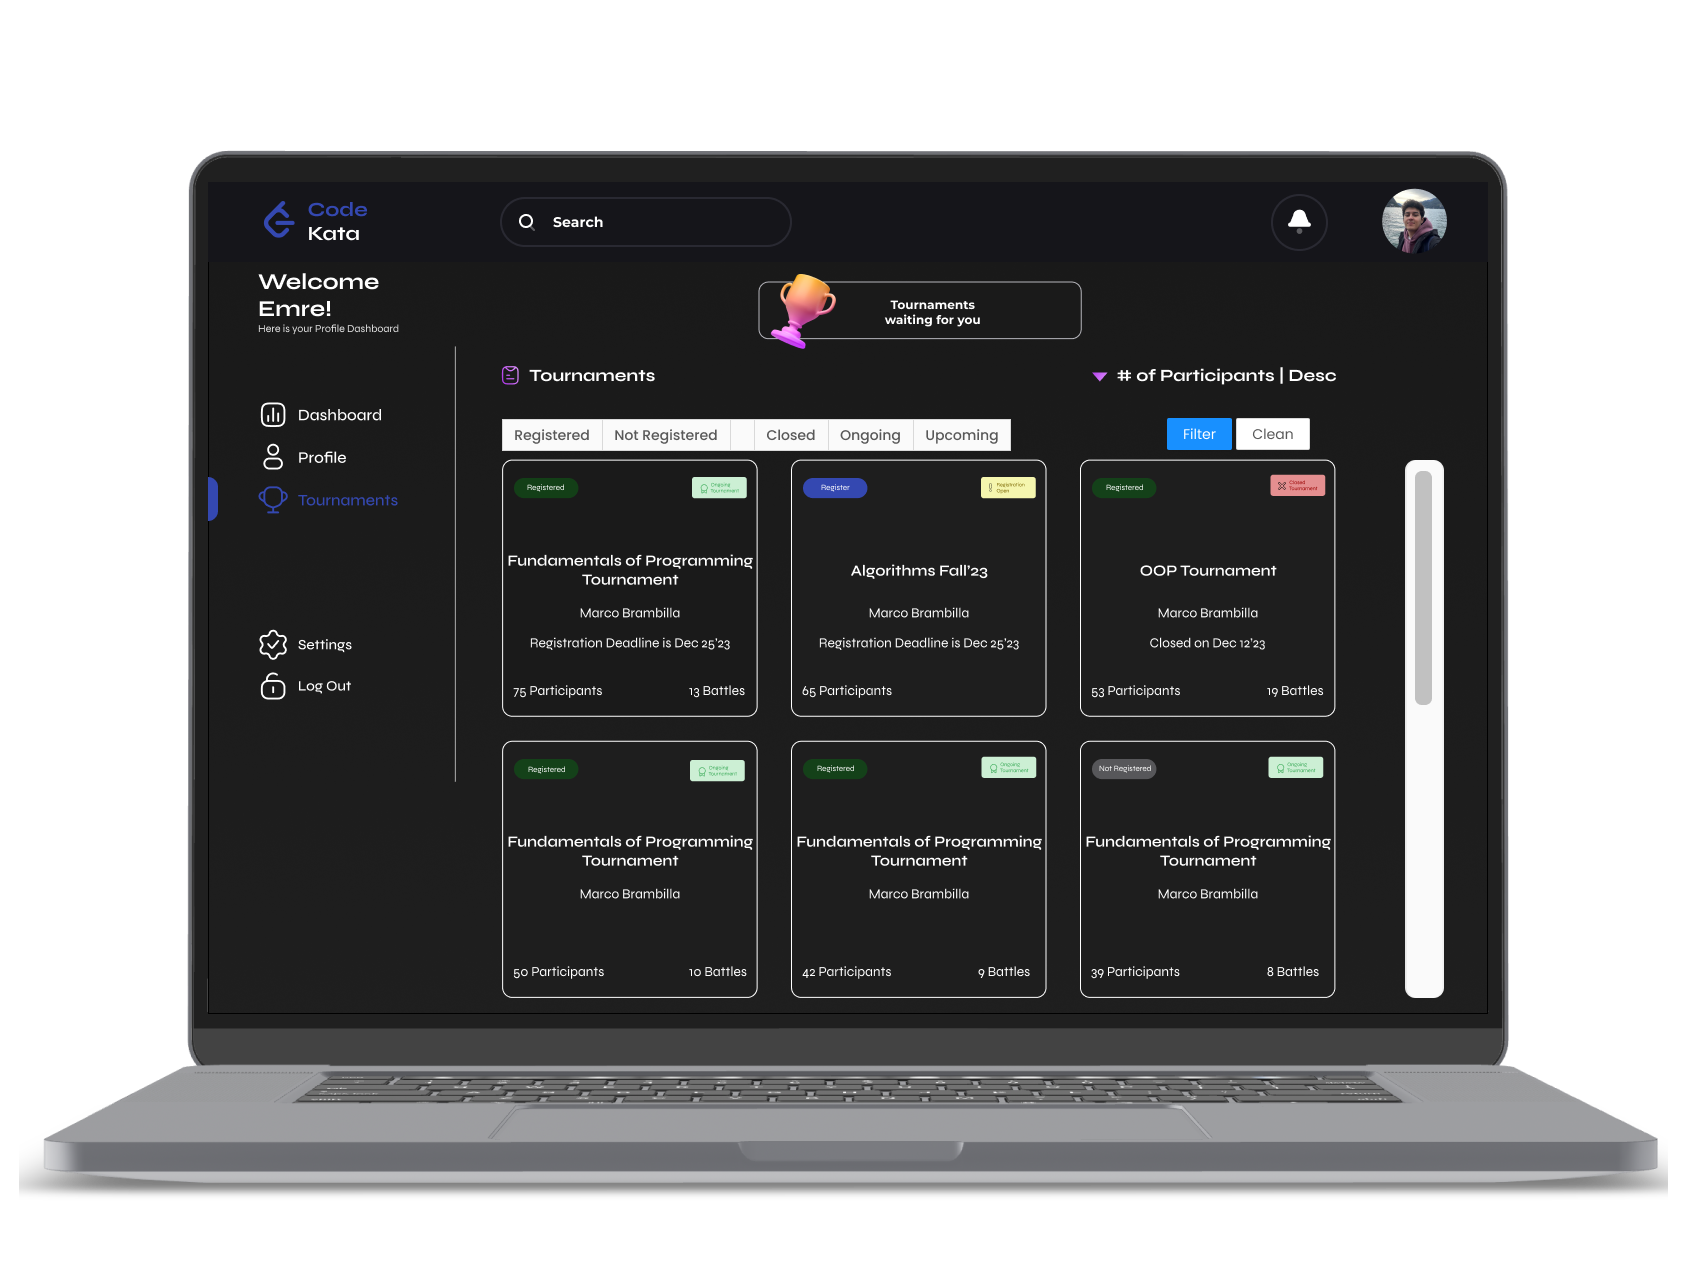
\includegraphics[scale=0.13]{Images/ui-ux/student_tournaments/student_tournaments_1.png}
    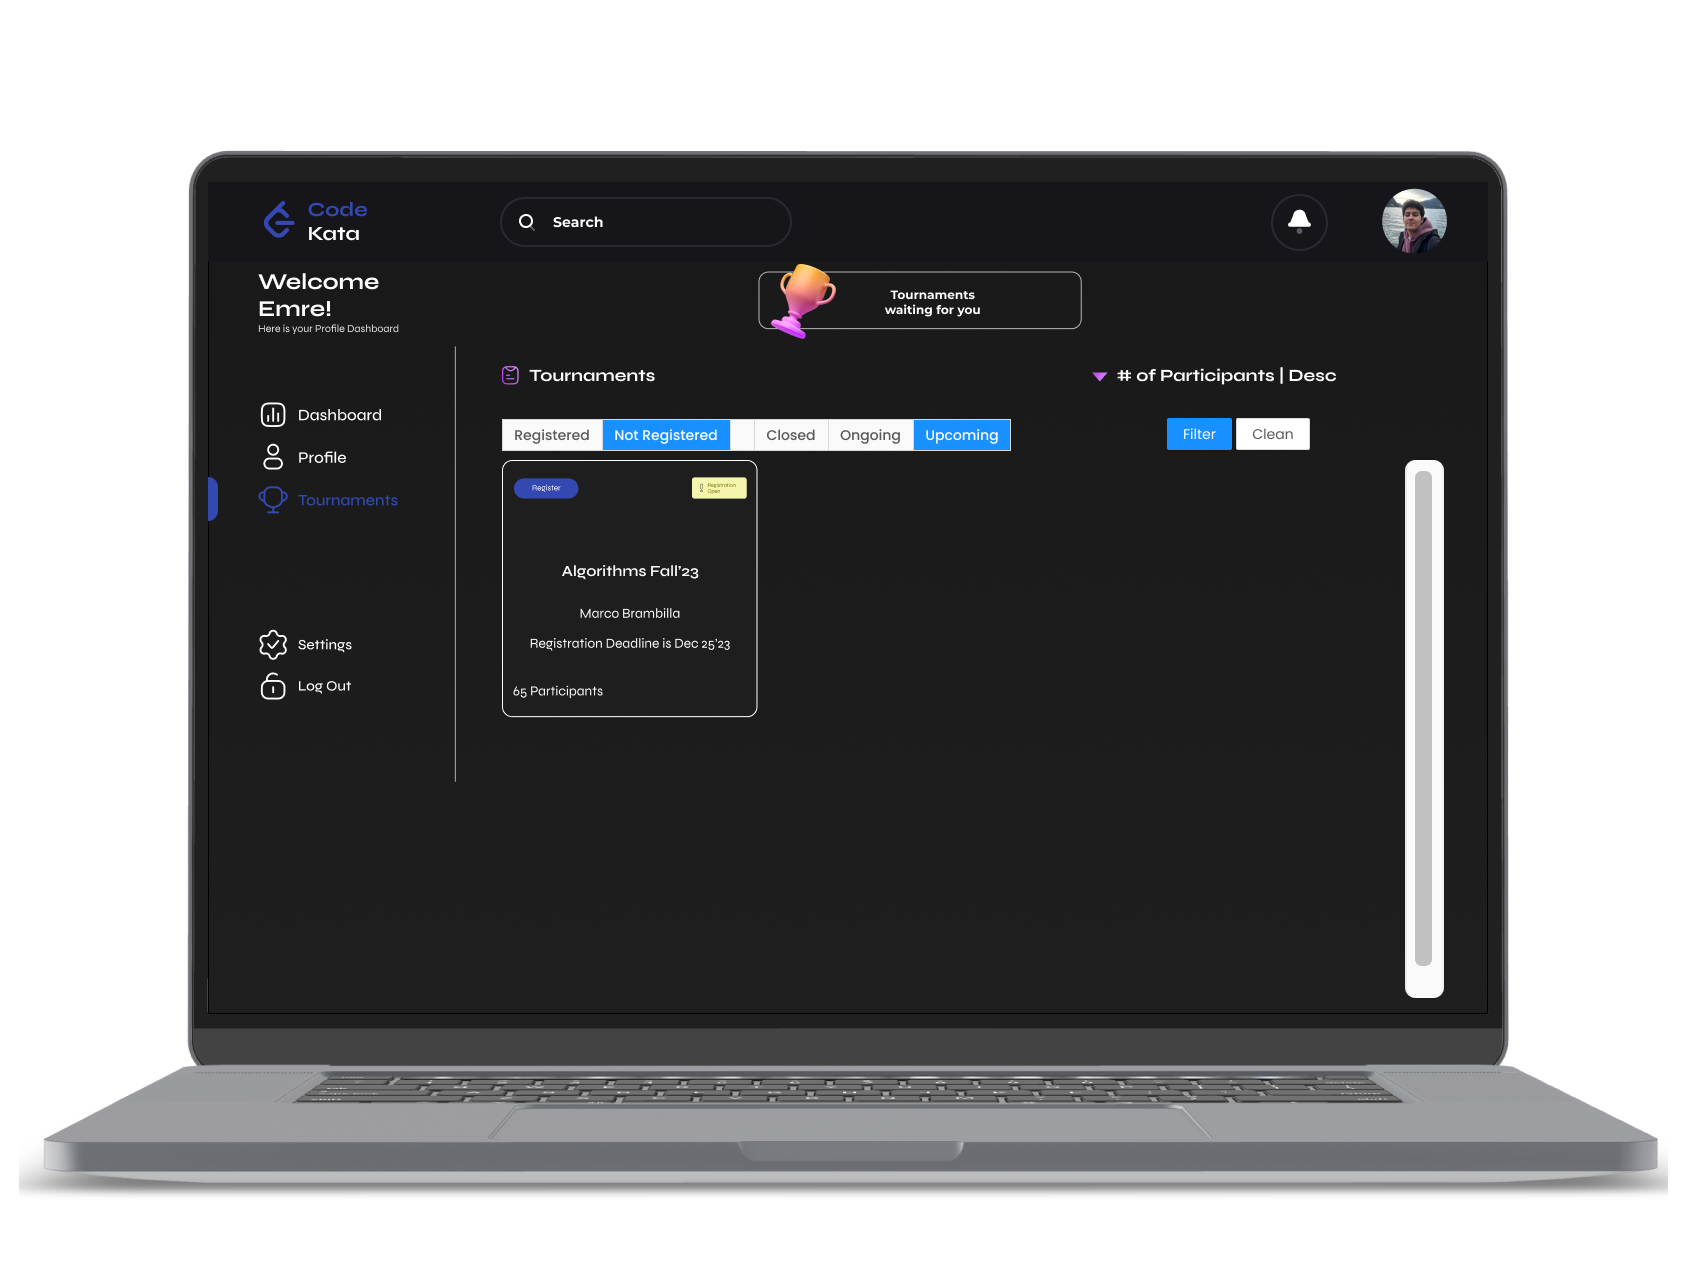
\includegraphics[scale=0.13]{Images/ui-ux/student_tournaments/student_tournaments_2.png}    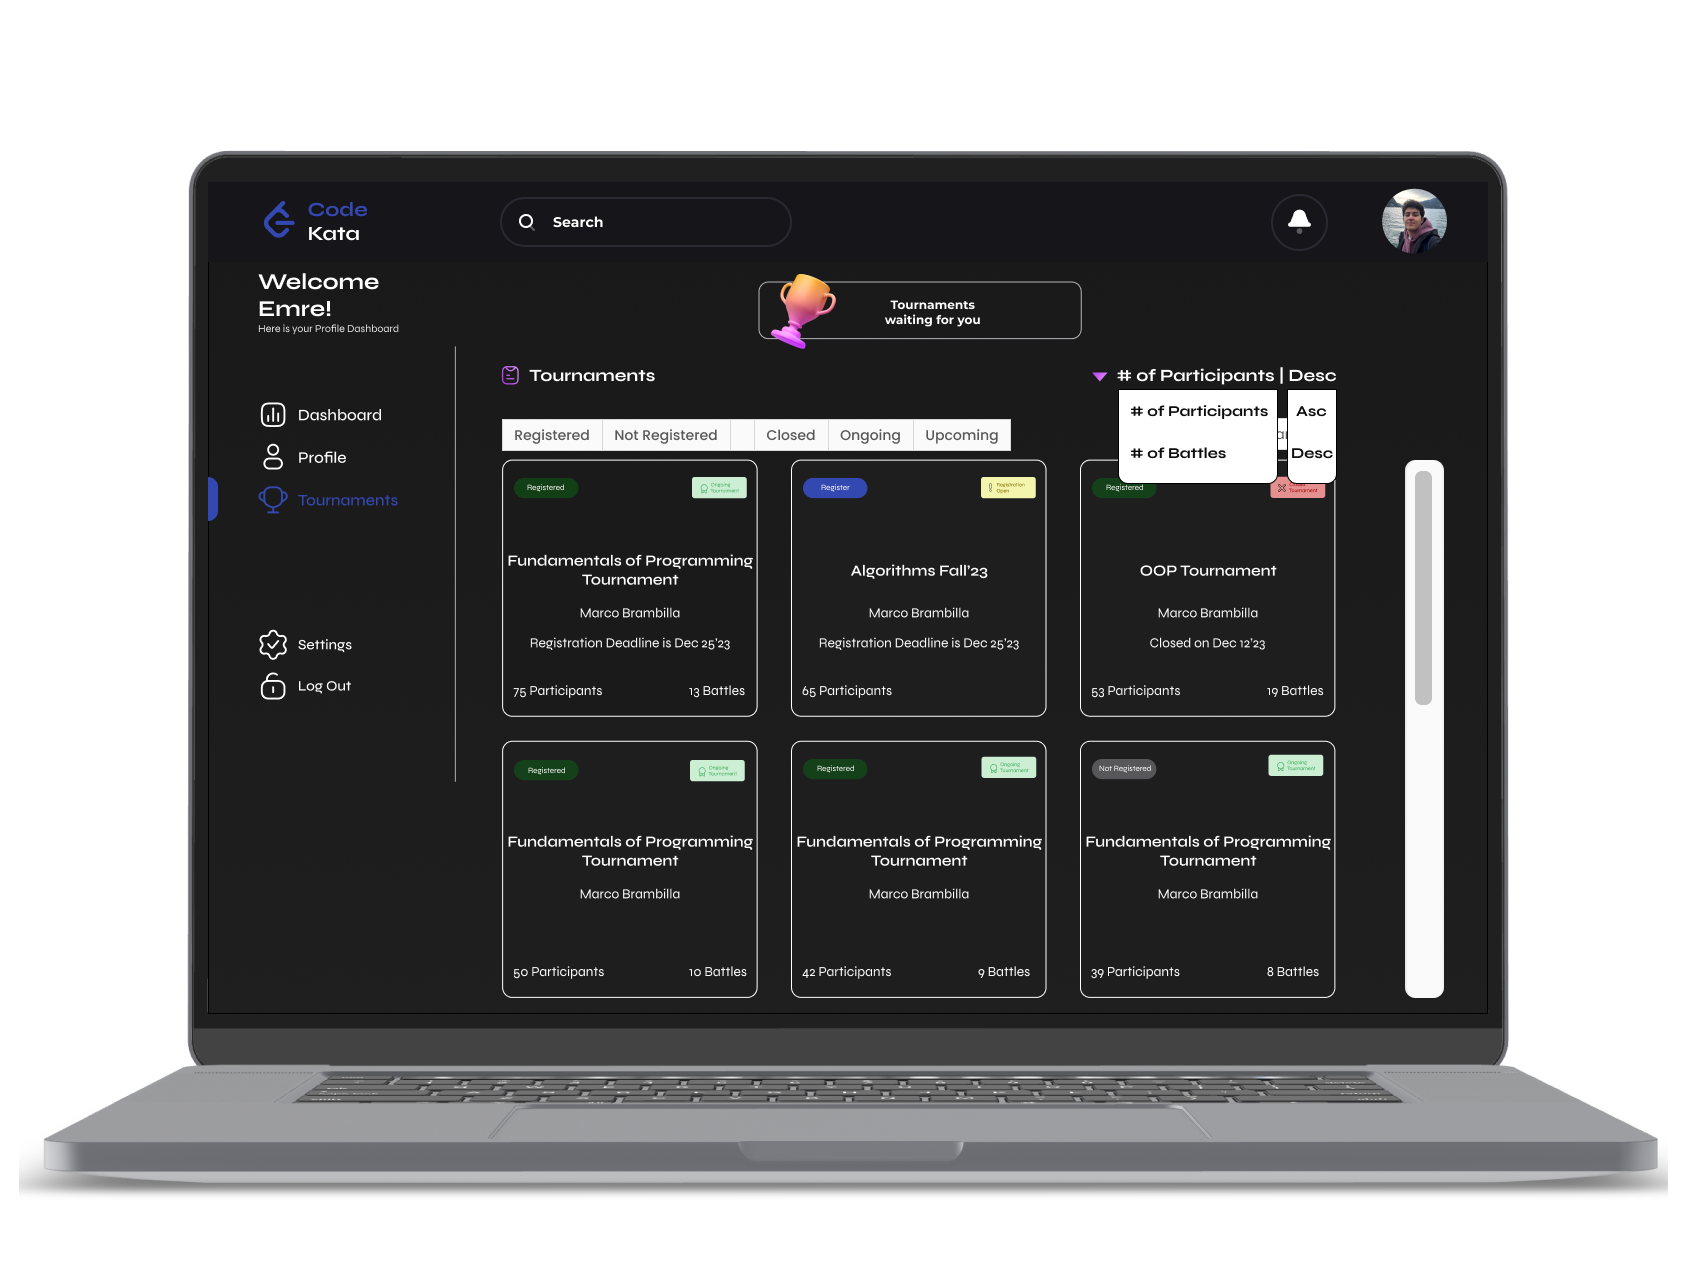
\includegraphics[scale=0.13]{Images/ui-ux/student_tournaments/student_tournaments_3.png}    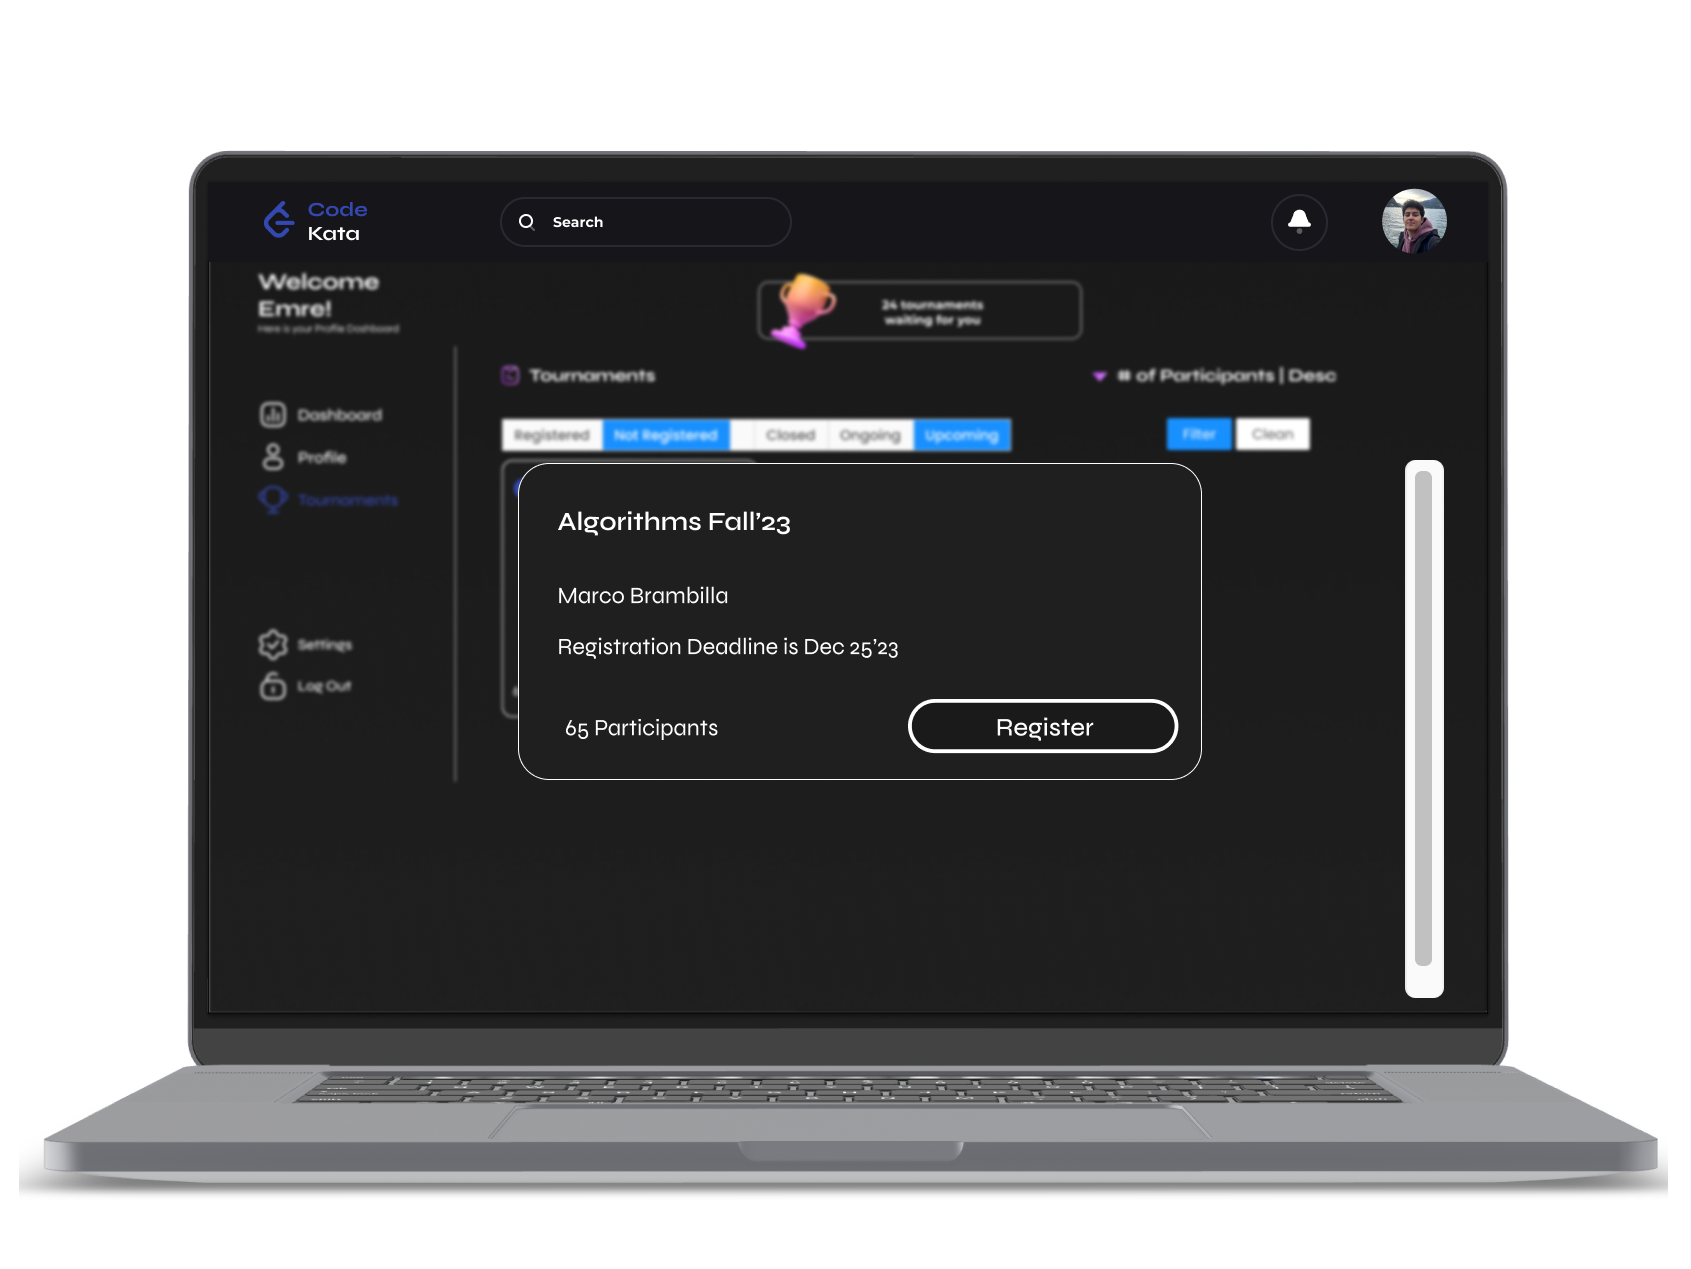
\includegraphics[scale=0.13]{Images/ui-ux/student_tournaments/student_tournaments_4.png}
        (d) Student Tournaments Page
\end{center}

\begin{center}
    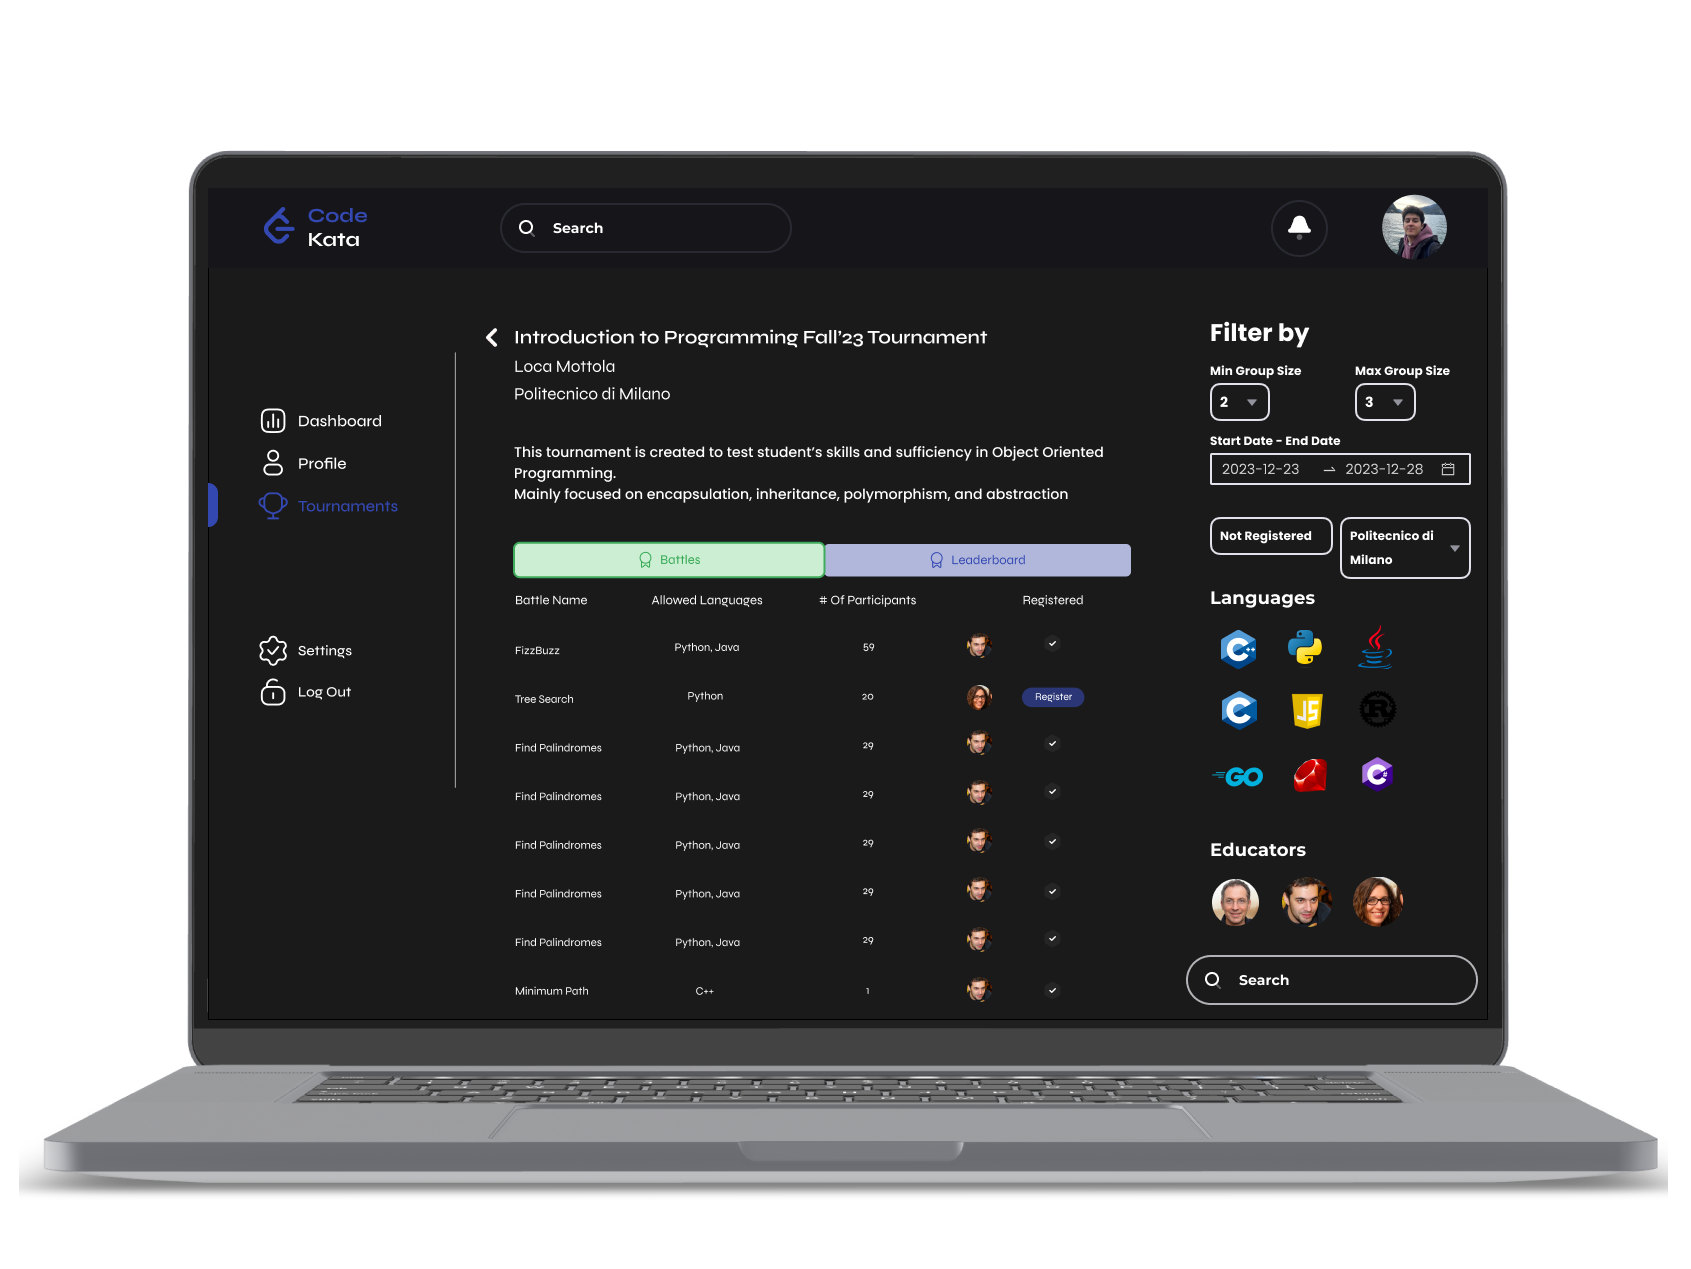
\includegraphics[scale=0.13]{Images/ui-ux/student_tournament/student_tournament_1.png}
    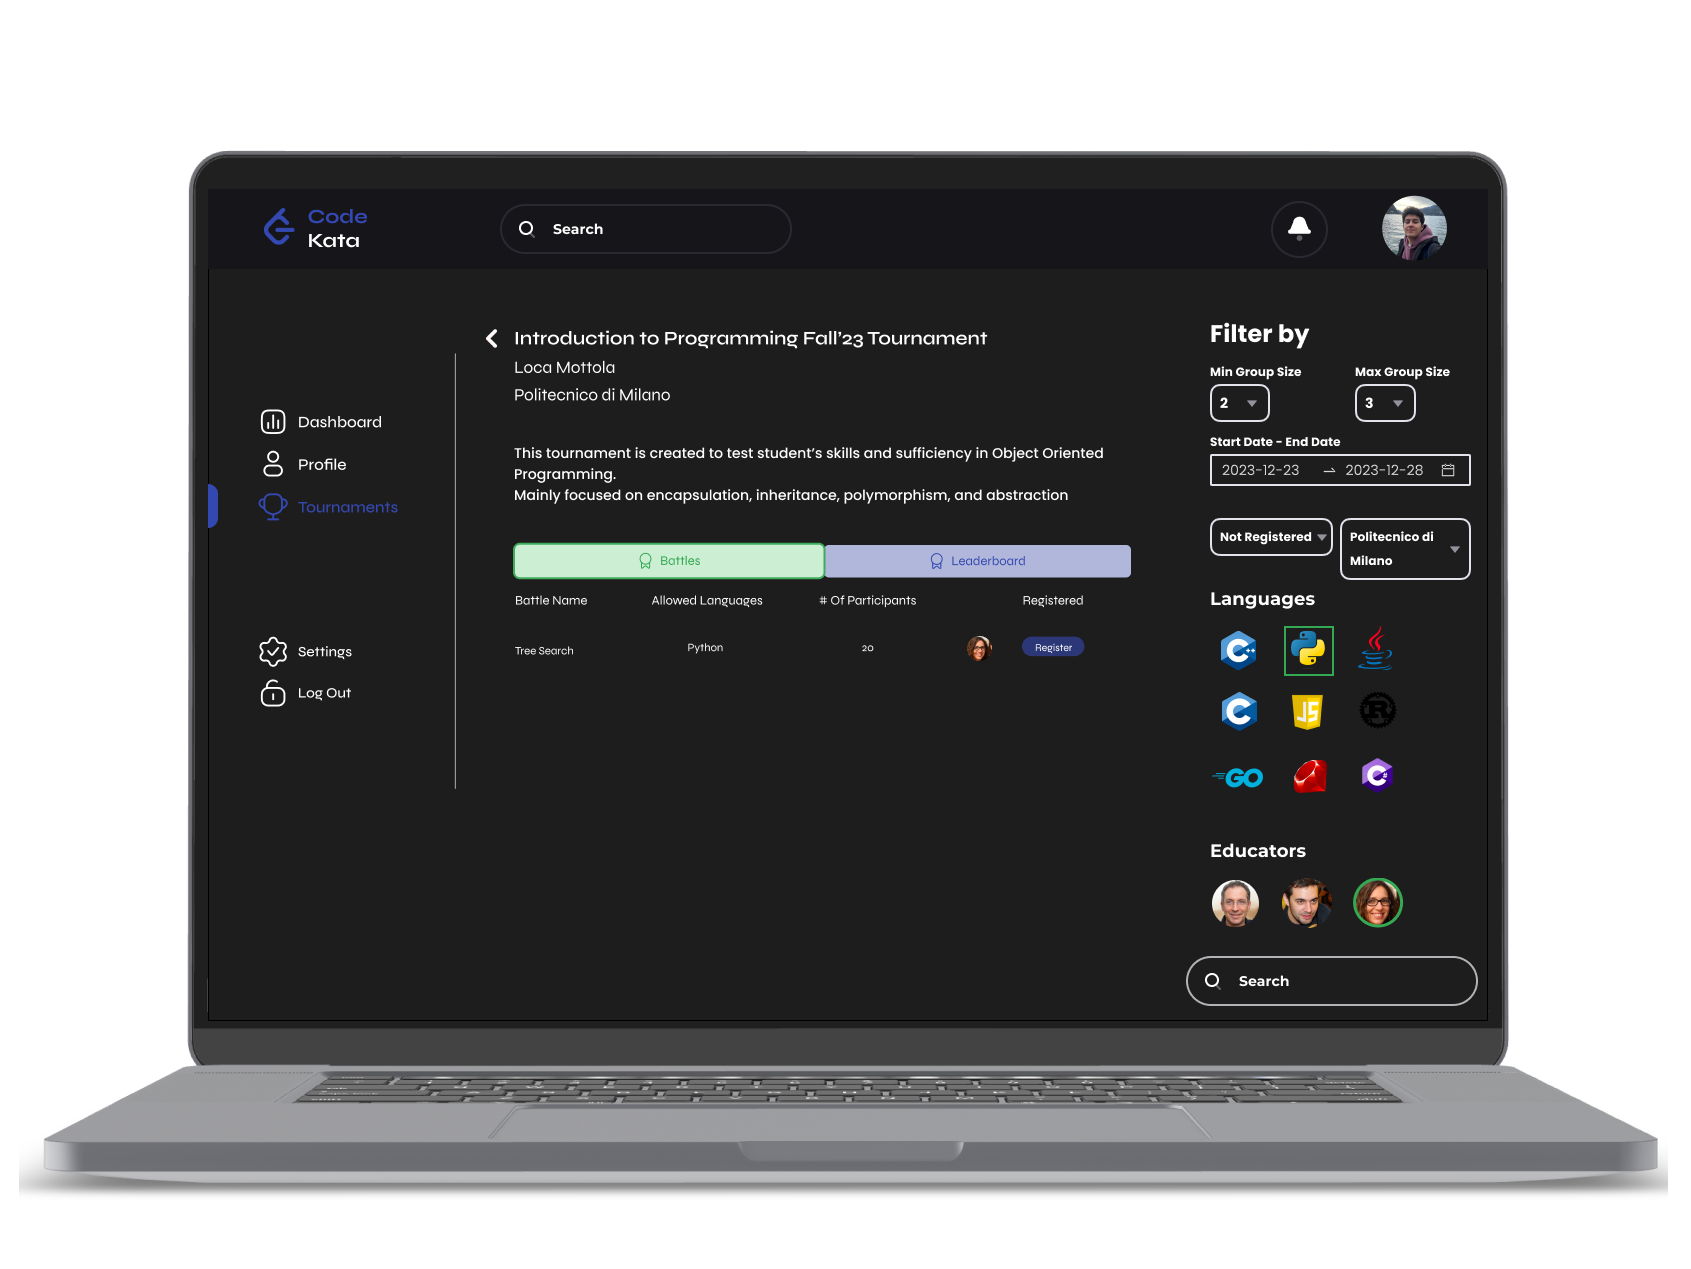
\includegraphics[scale=0.13]{Images/ui-ux/student_tournament/student_tournament_2.png}    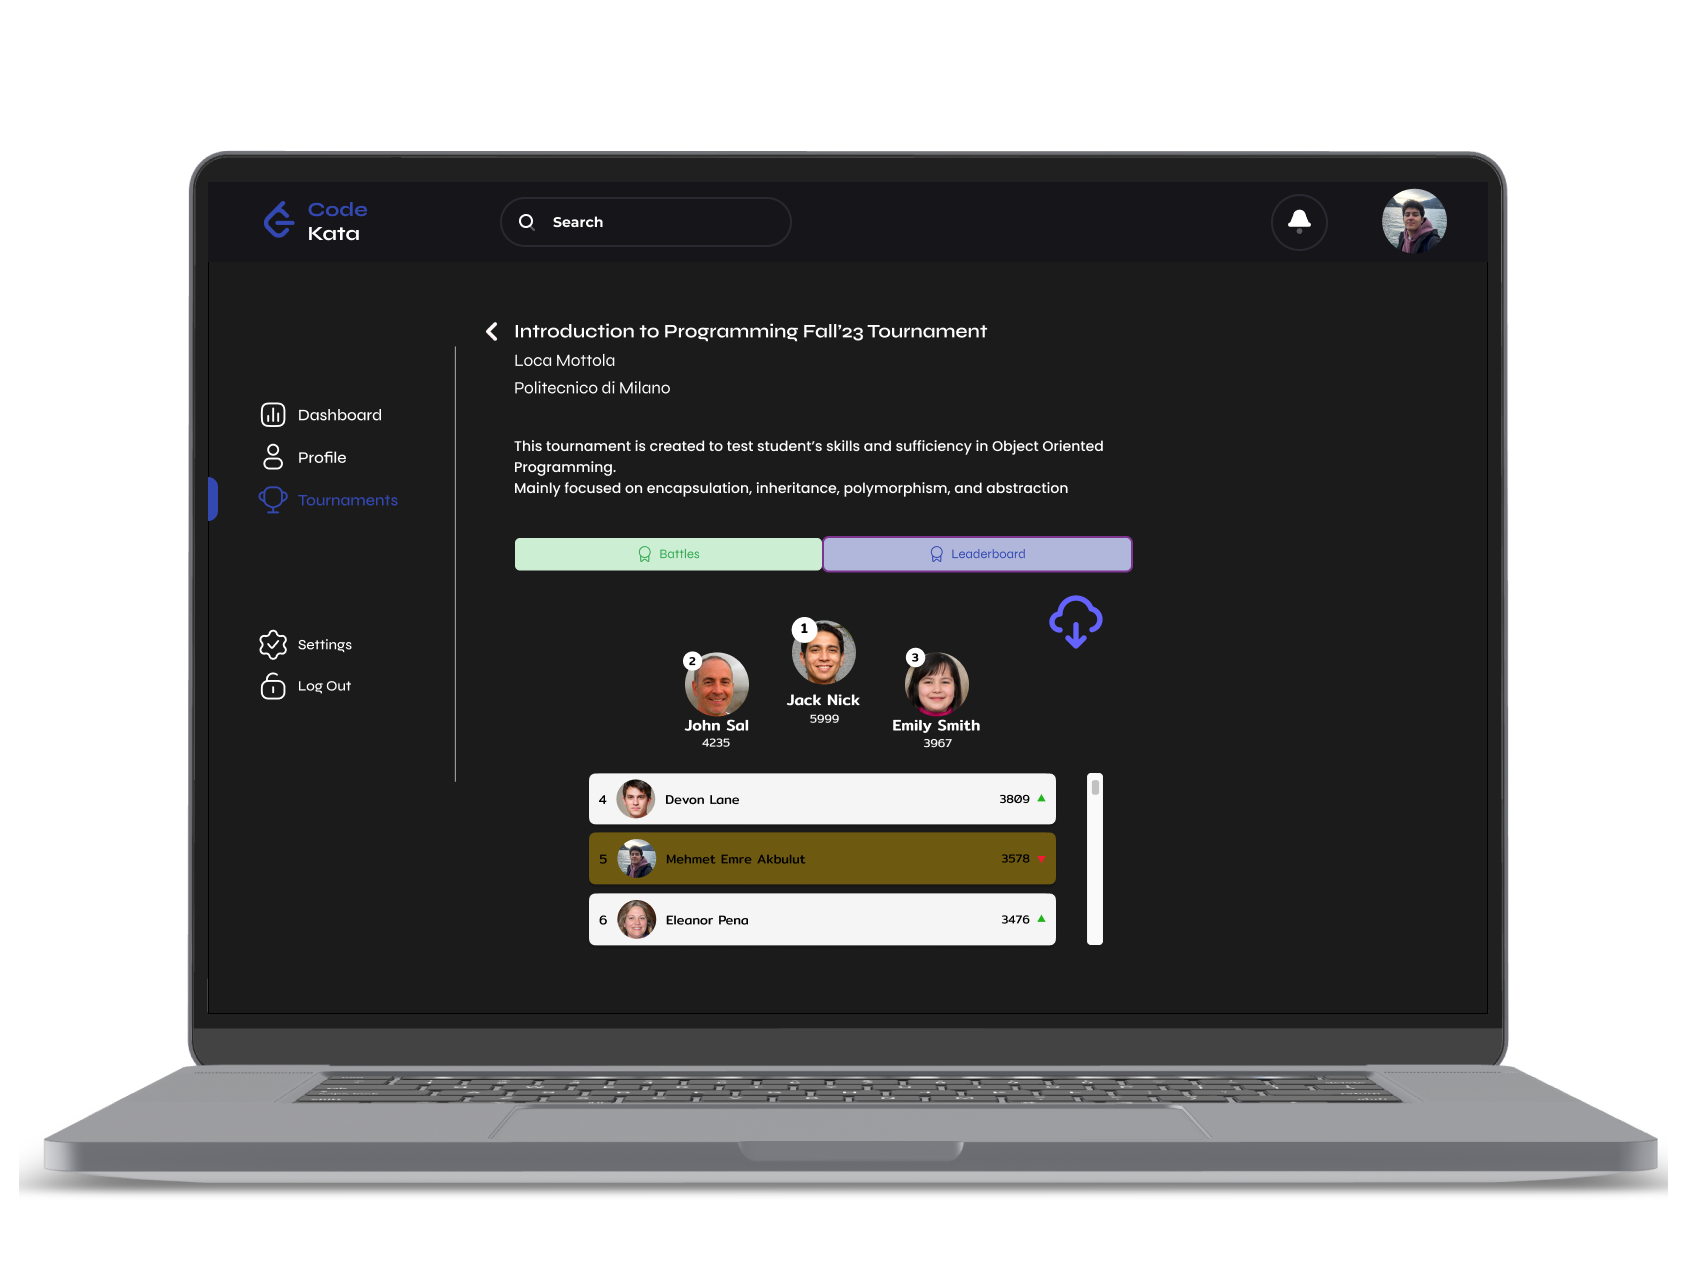
\includegraphics[scale=0.13]{Images/ui-ux/student_tournament/student_tournament_3.png} 
    \\ (e) Student visits a Tournament
\end{center}
\newpage
\begin{center}
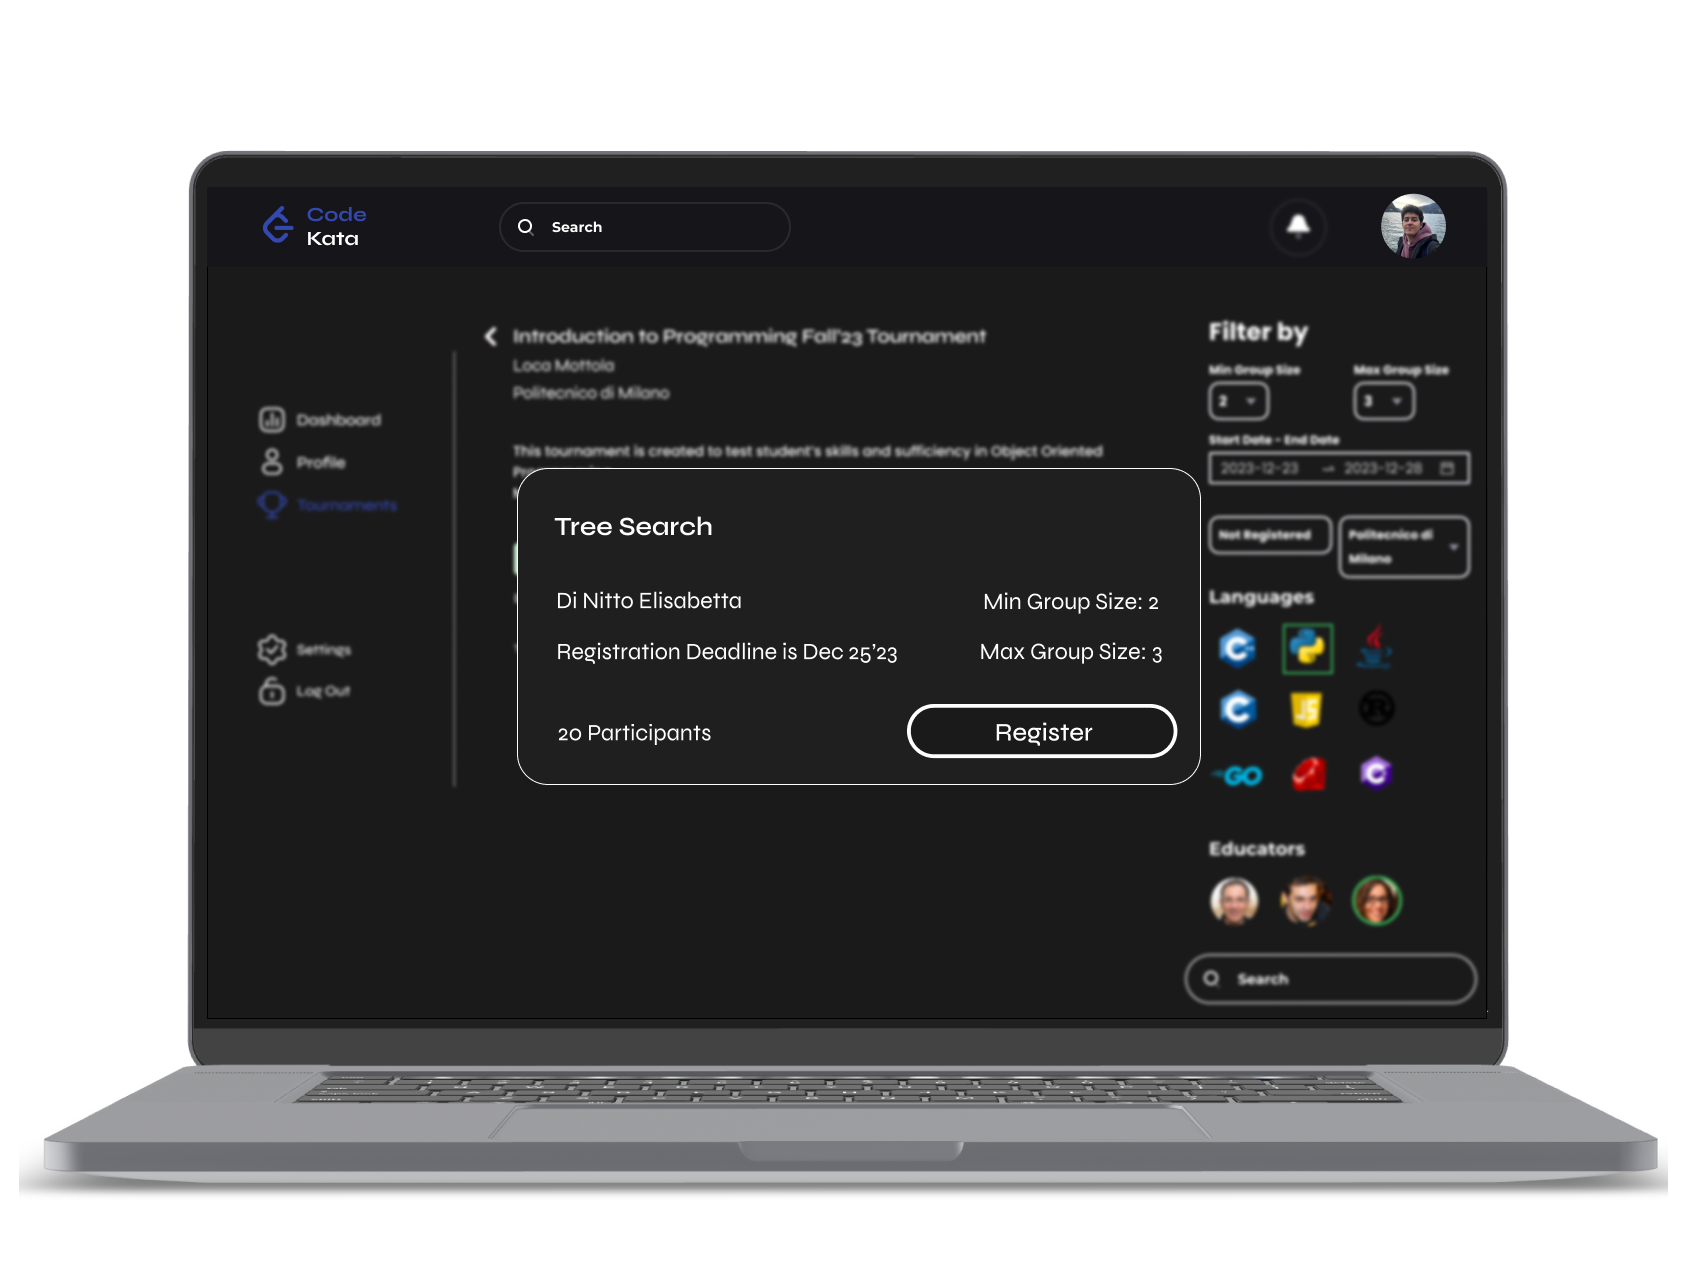
\includegraphics[scale=0.13]{Images/ui-ux/student_battle_register/student_battle_register_1.png}
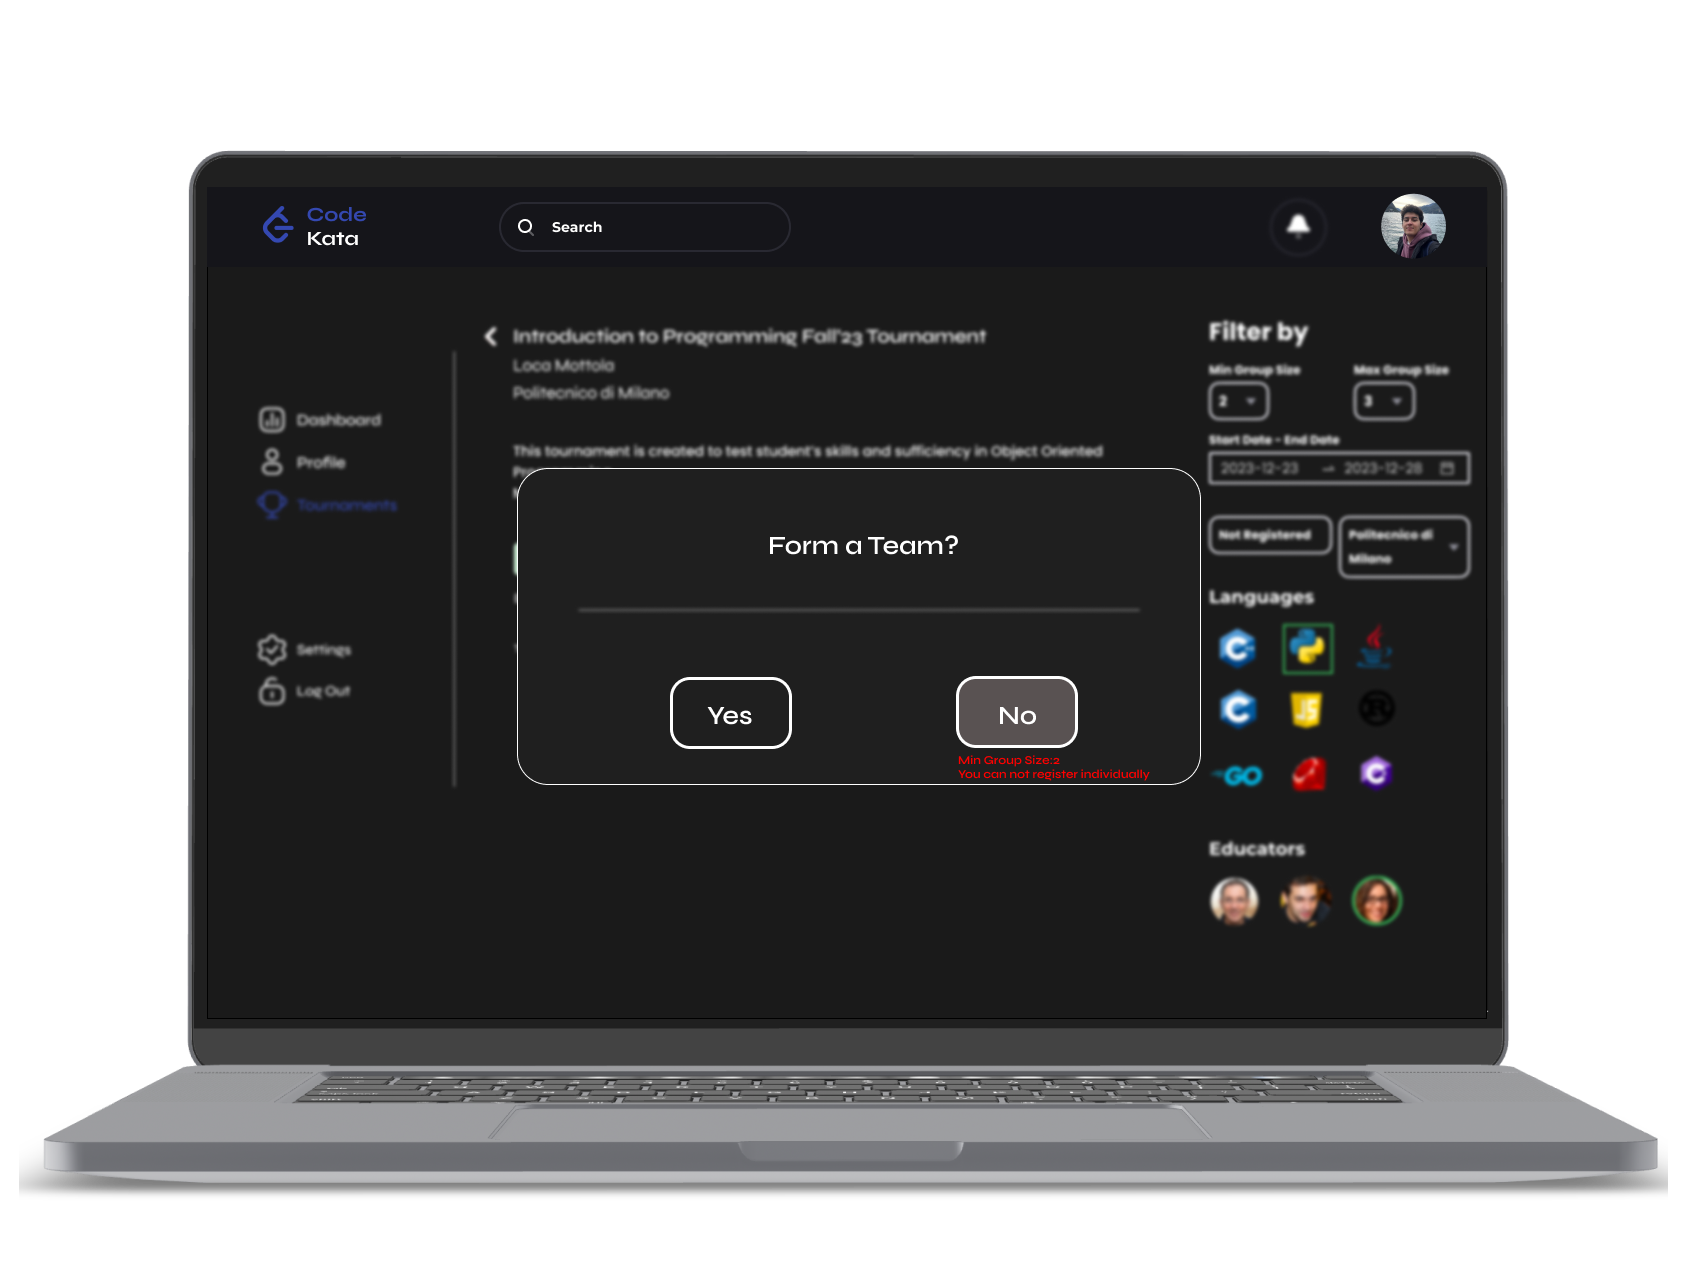
\includegraphics[scale=0.13]{Images/ui-ux/student_battle_register/student_battle_register_2.png}
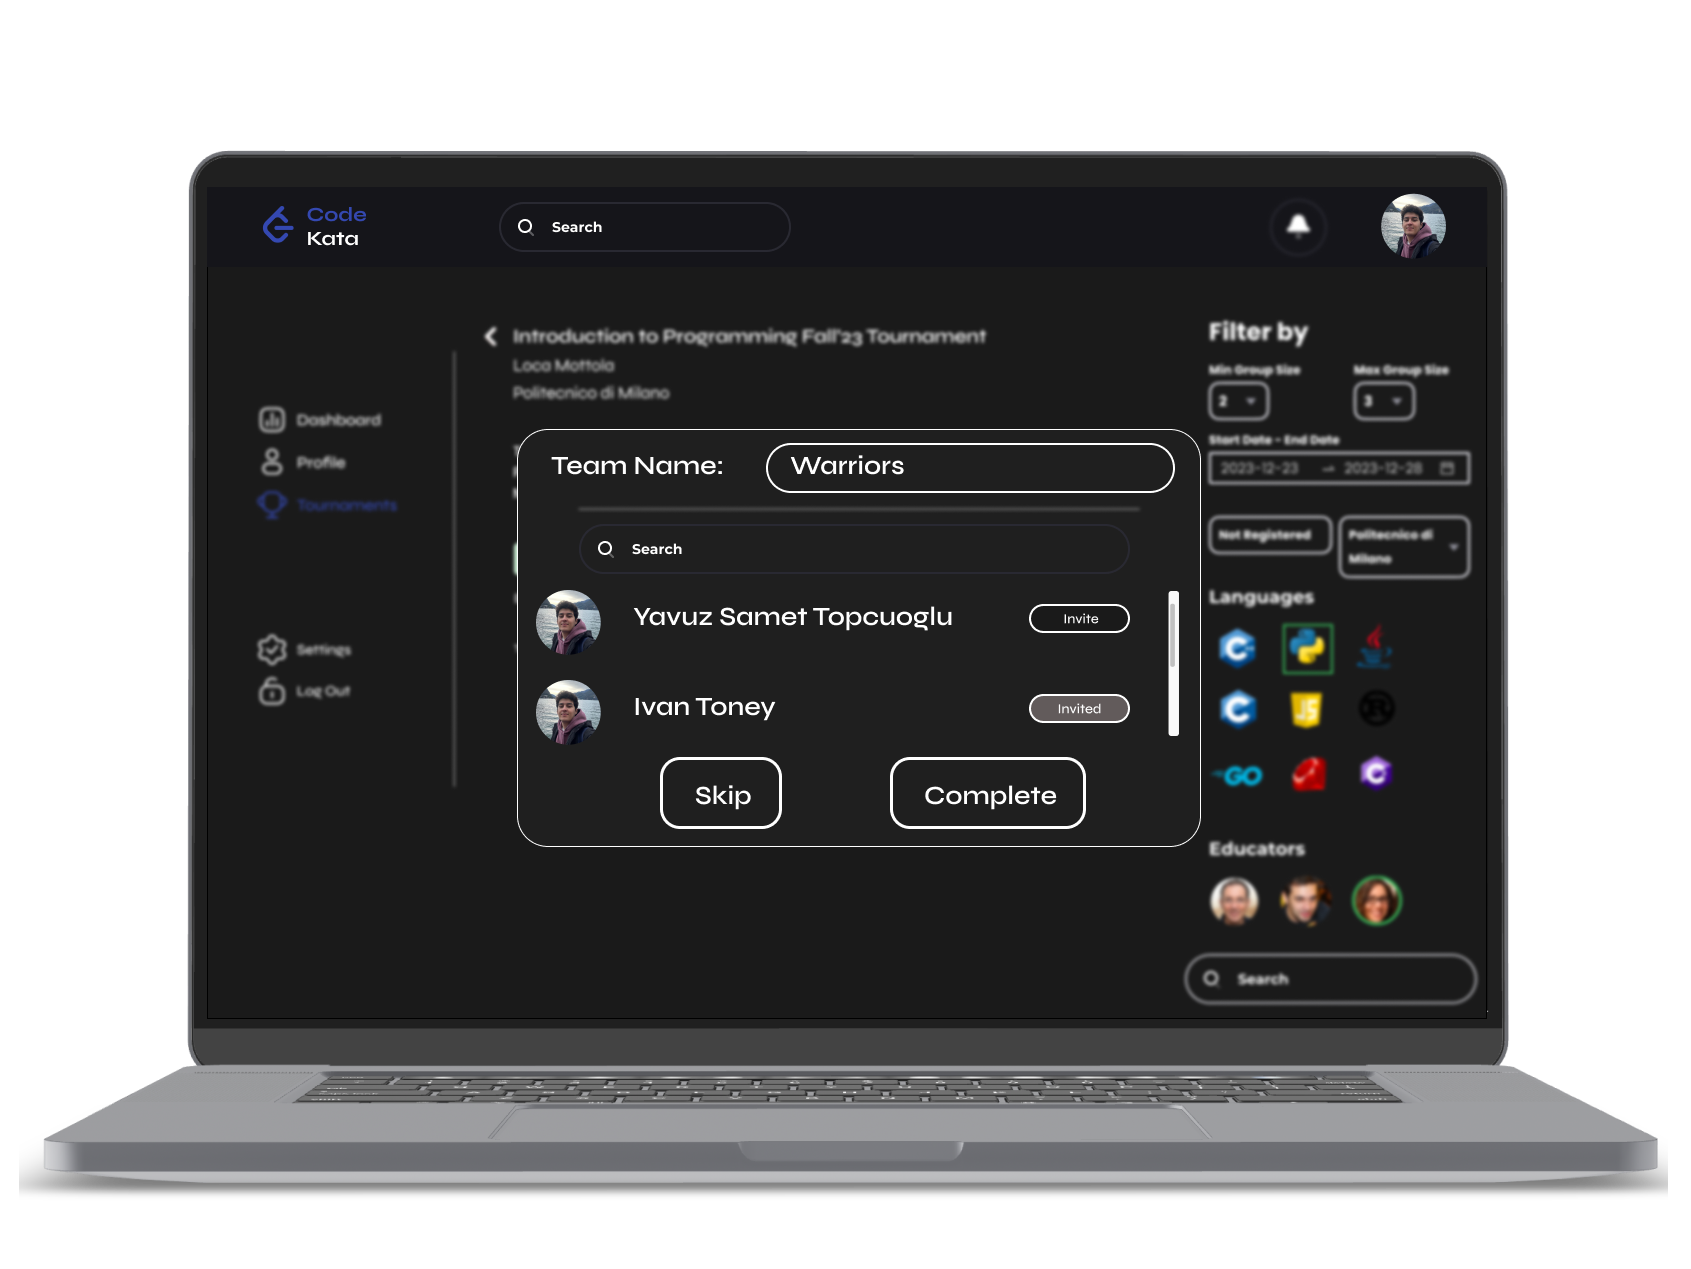
\includegraphics[scale=0.13]{Images/ui-ux/student_battle_register/student_battle_register_3.png}
\\ (f) Student Registers Battle
\end{center}
\newpage
\begin{center}
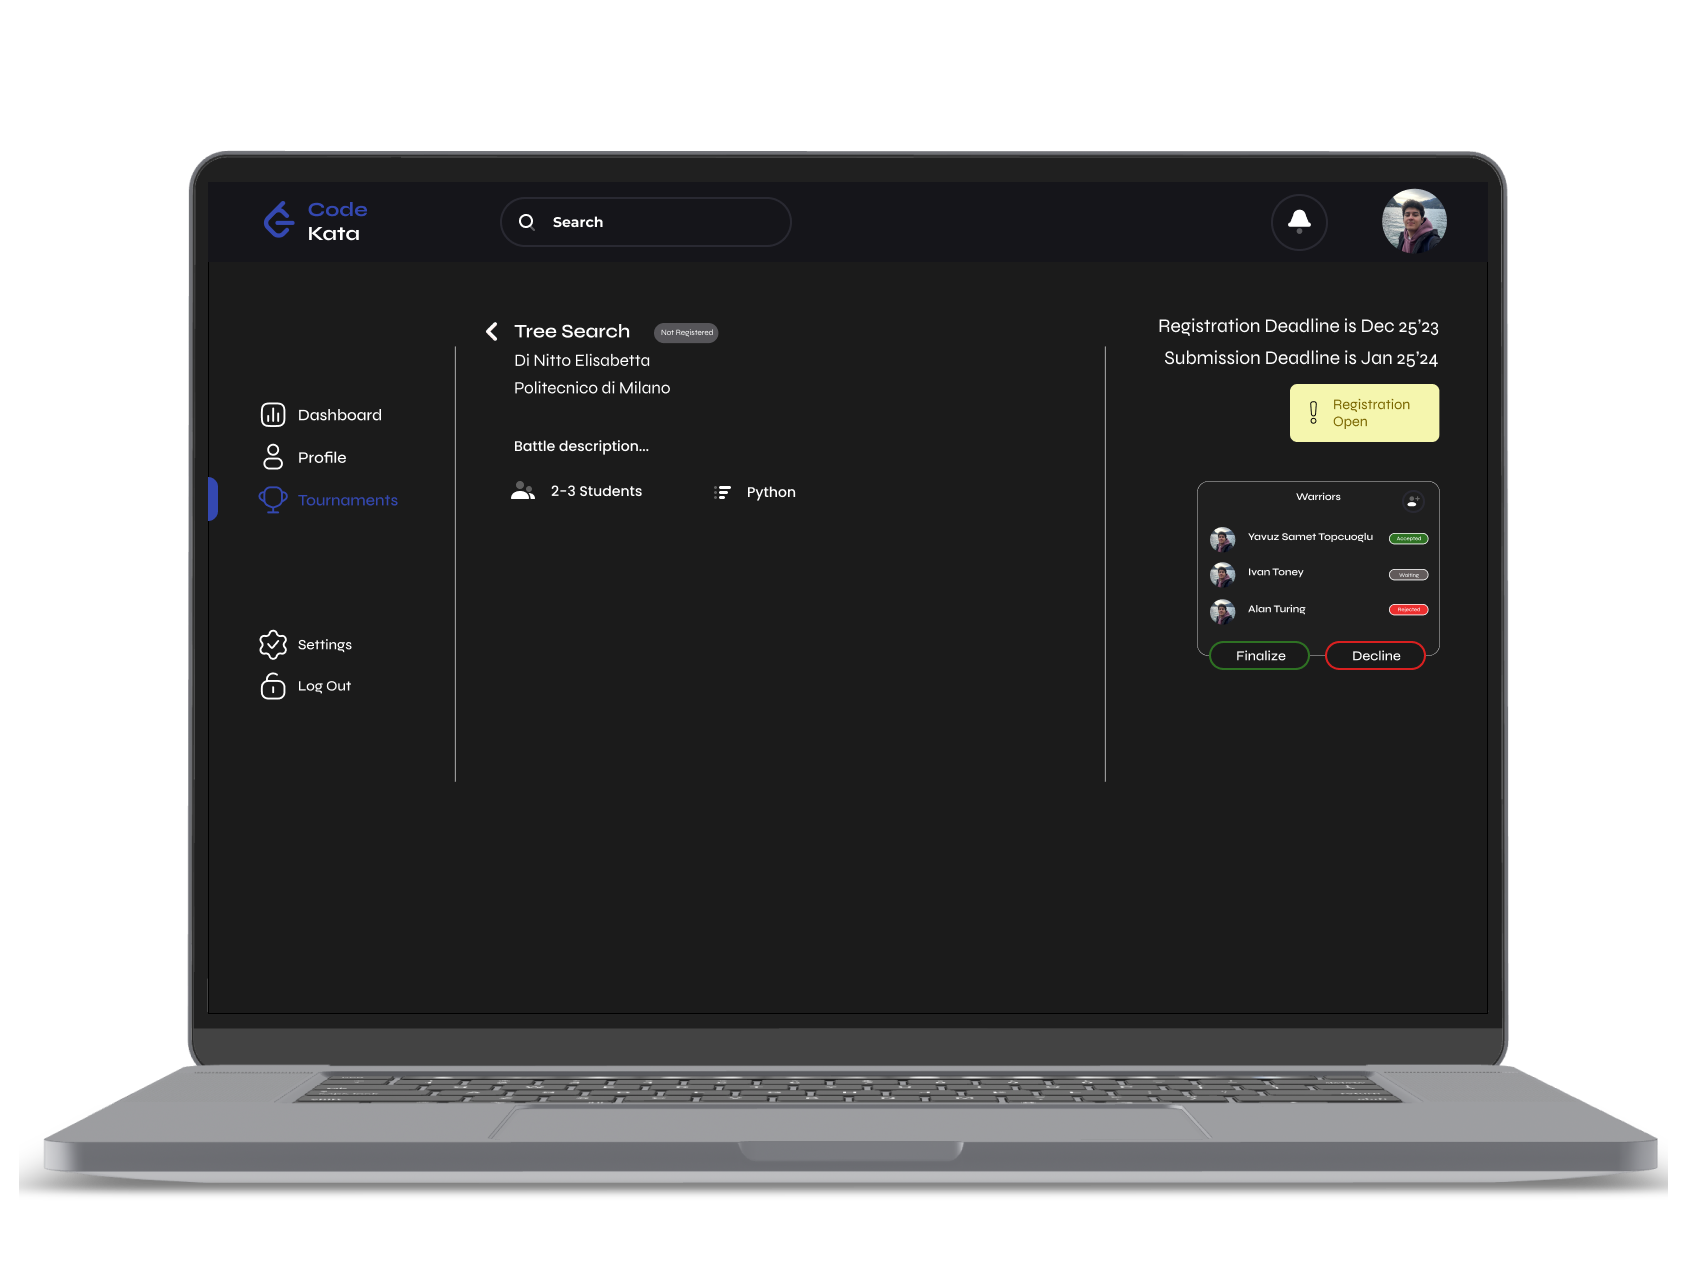
\includegraphics[scale=0.13]{Images/ui-ux/student_battle/student_battle_1.png}
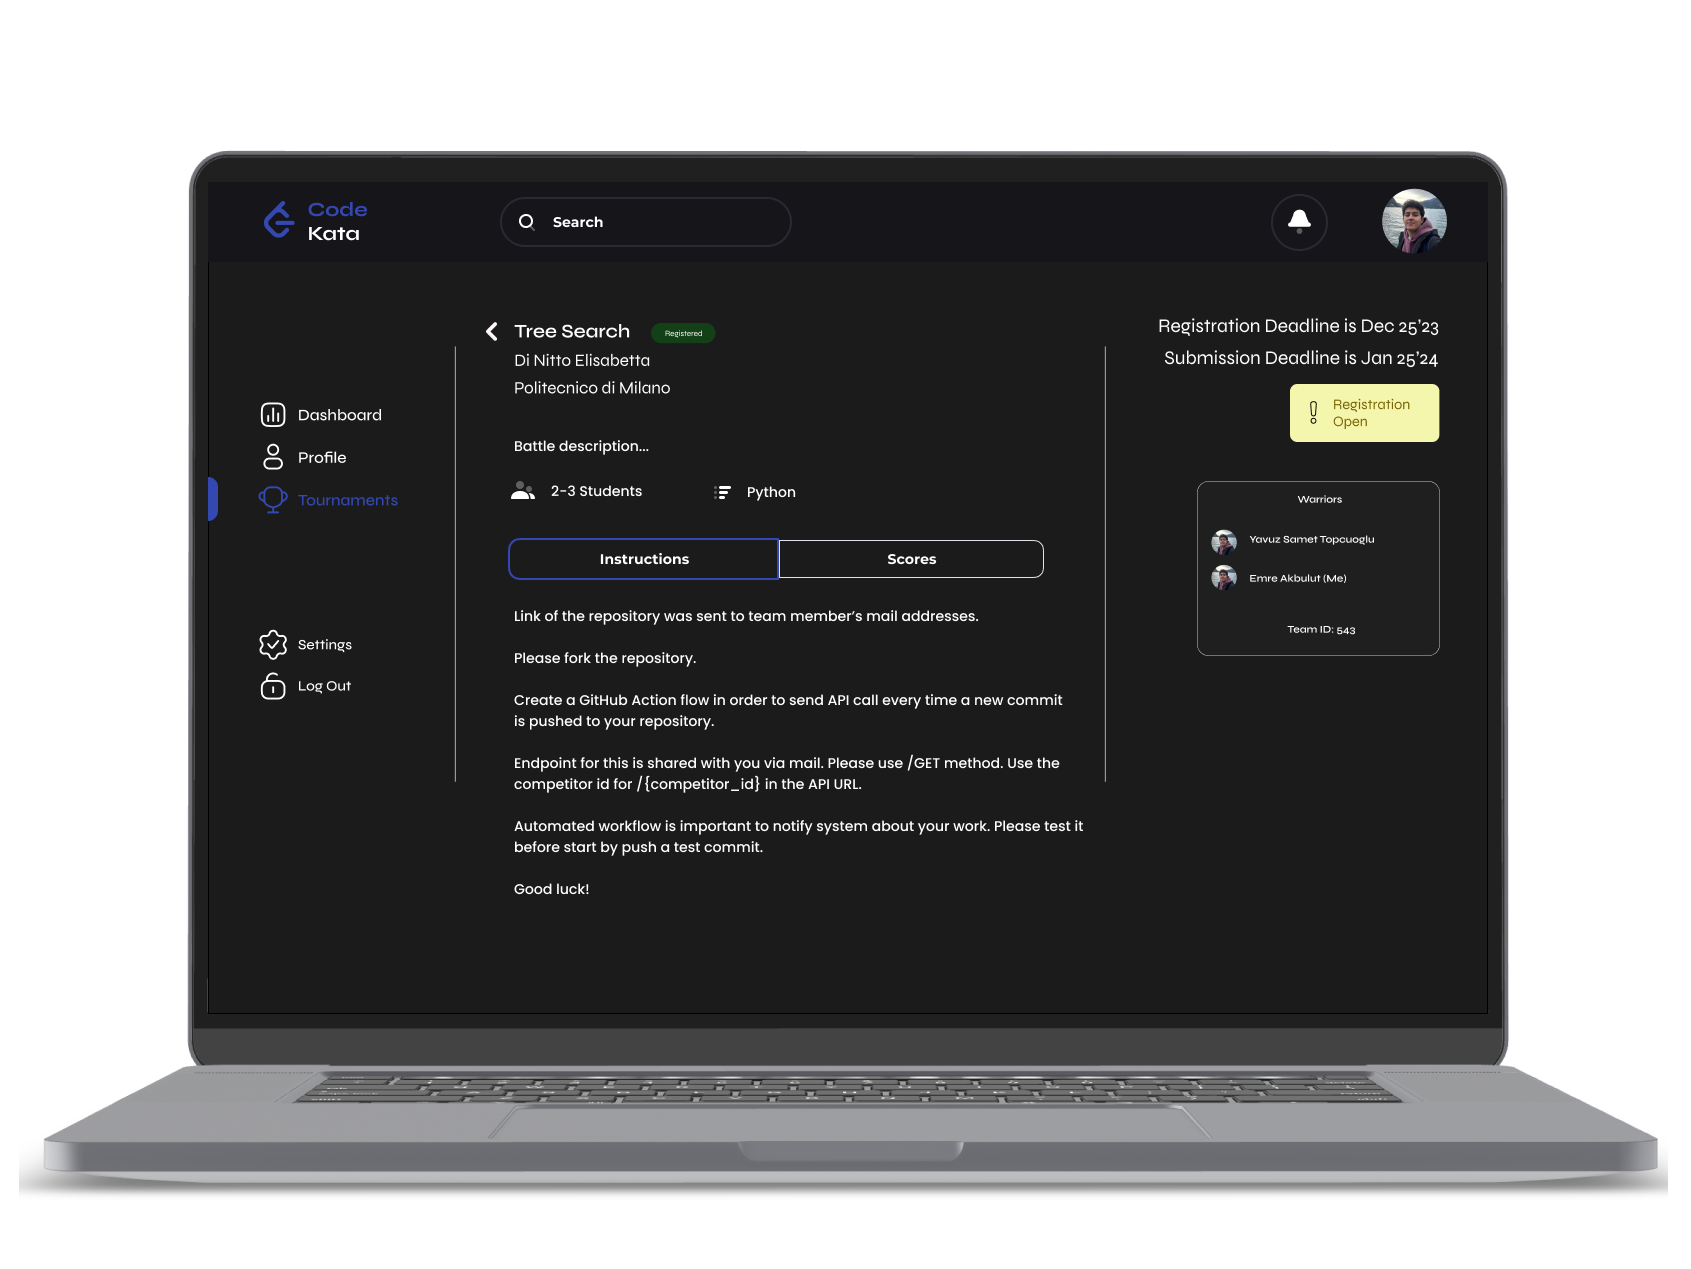
\includegraphics[scale=0.13]{Images/ui-ux/student_battle/student_battle_2.png}
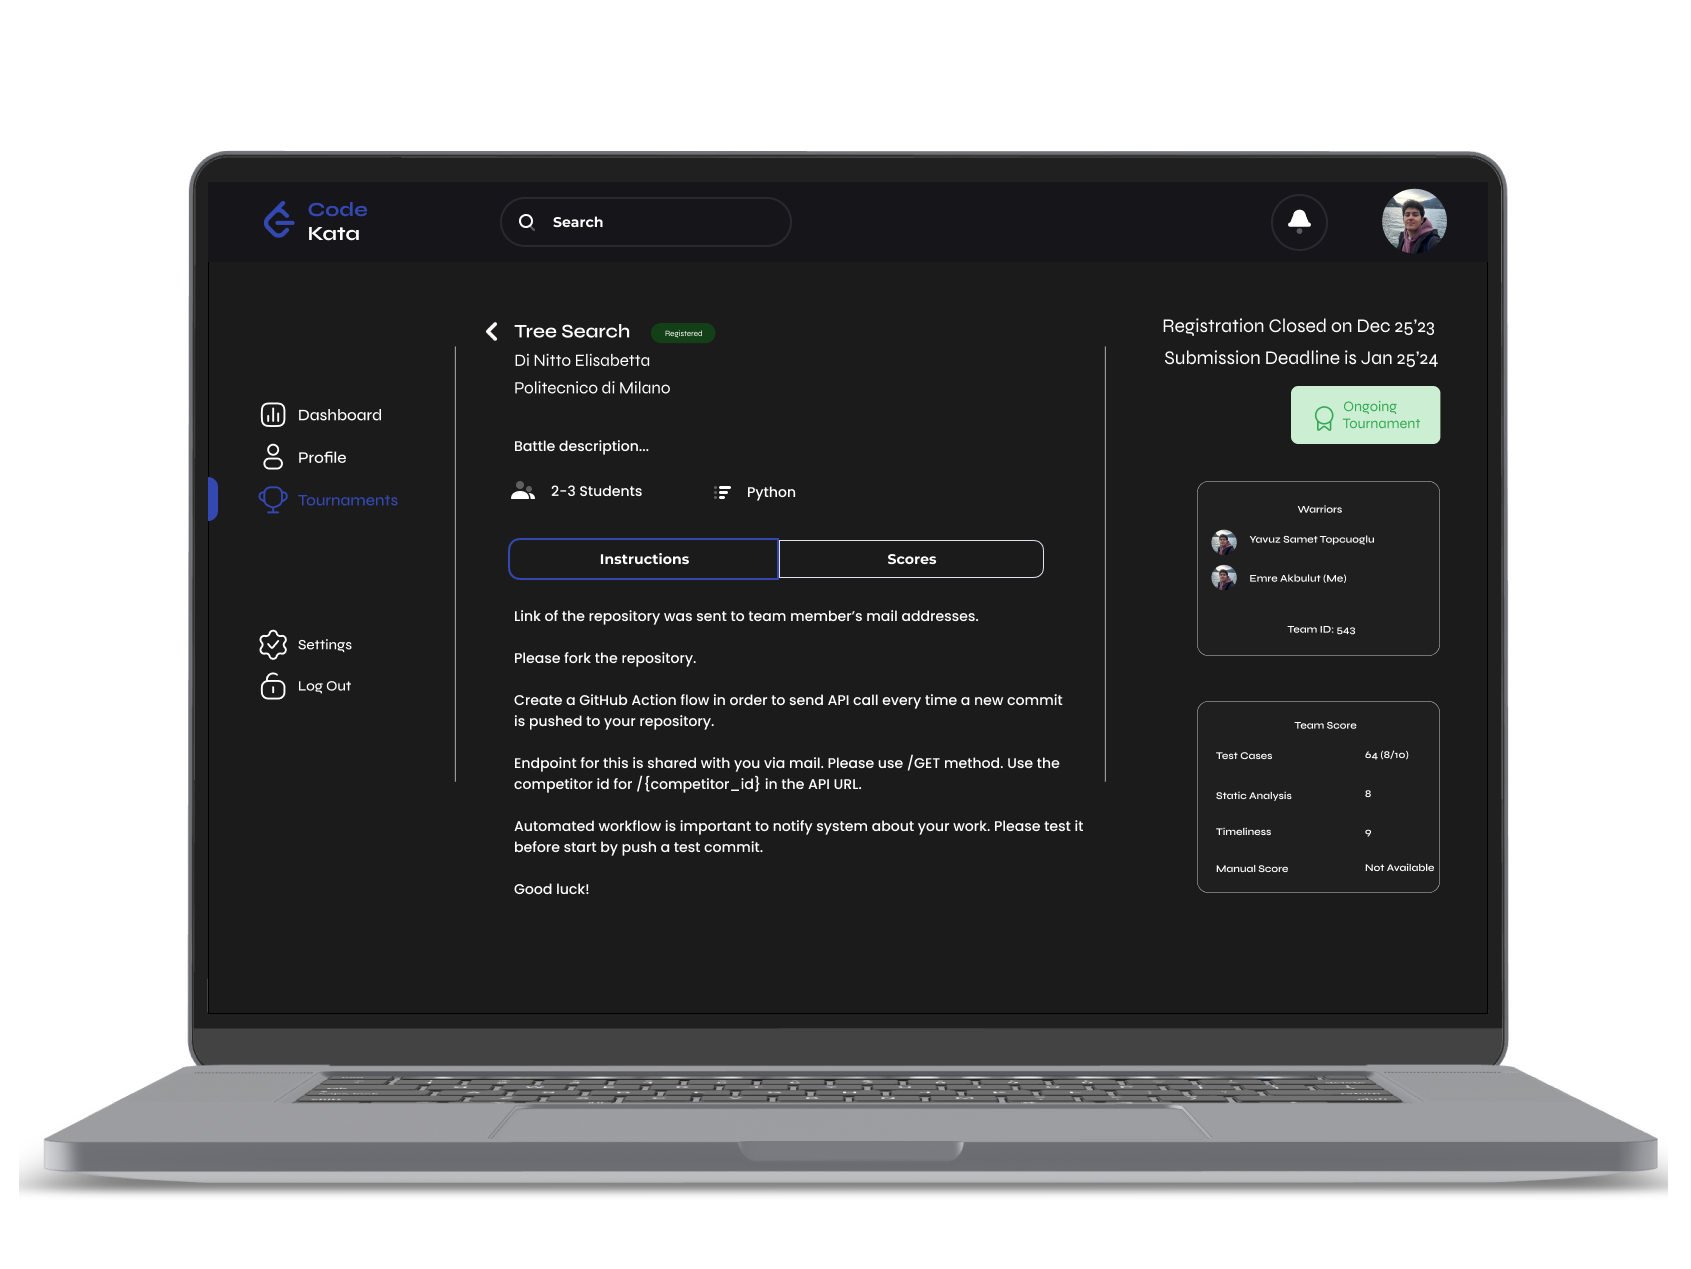
\includegraphics[scale=0.13]{Images/ui-ux/student_battle/student_battle_3.png}
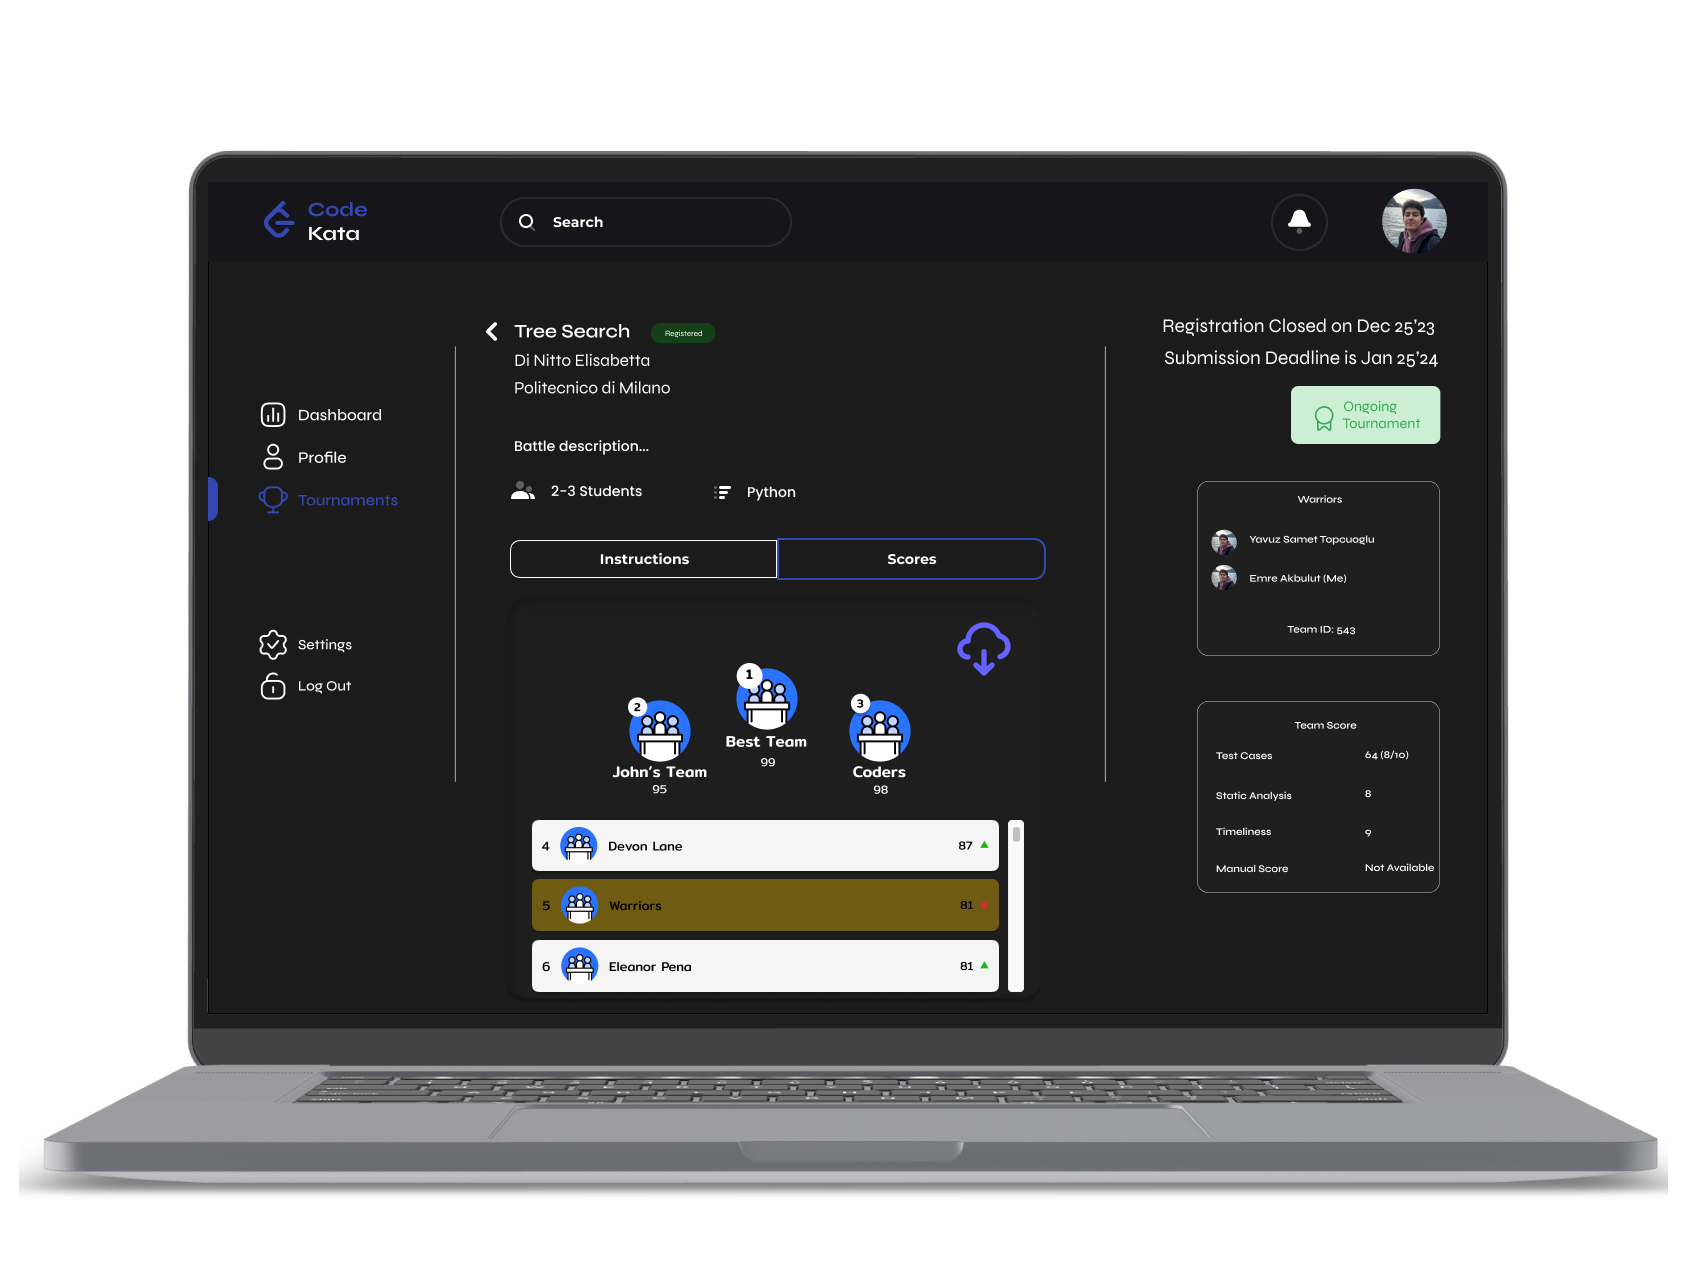
\includegraphics[scale=0.13]{Images/ui-ux/student_battle/student_battle_4.png}
      (g) Battle Screen for Student
\end{center}

\begin{center}
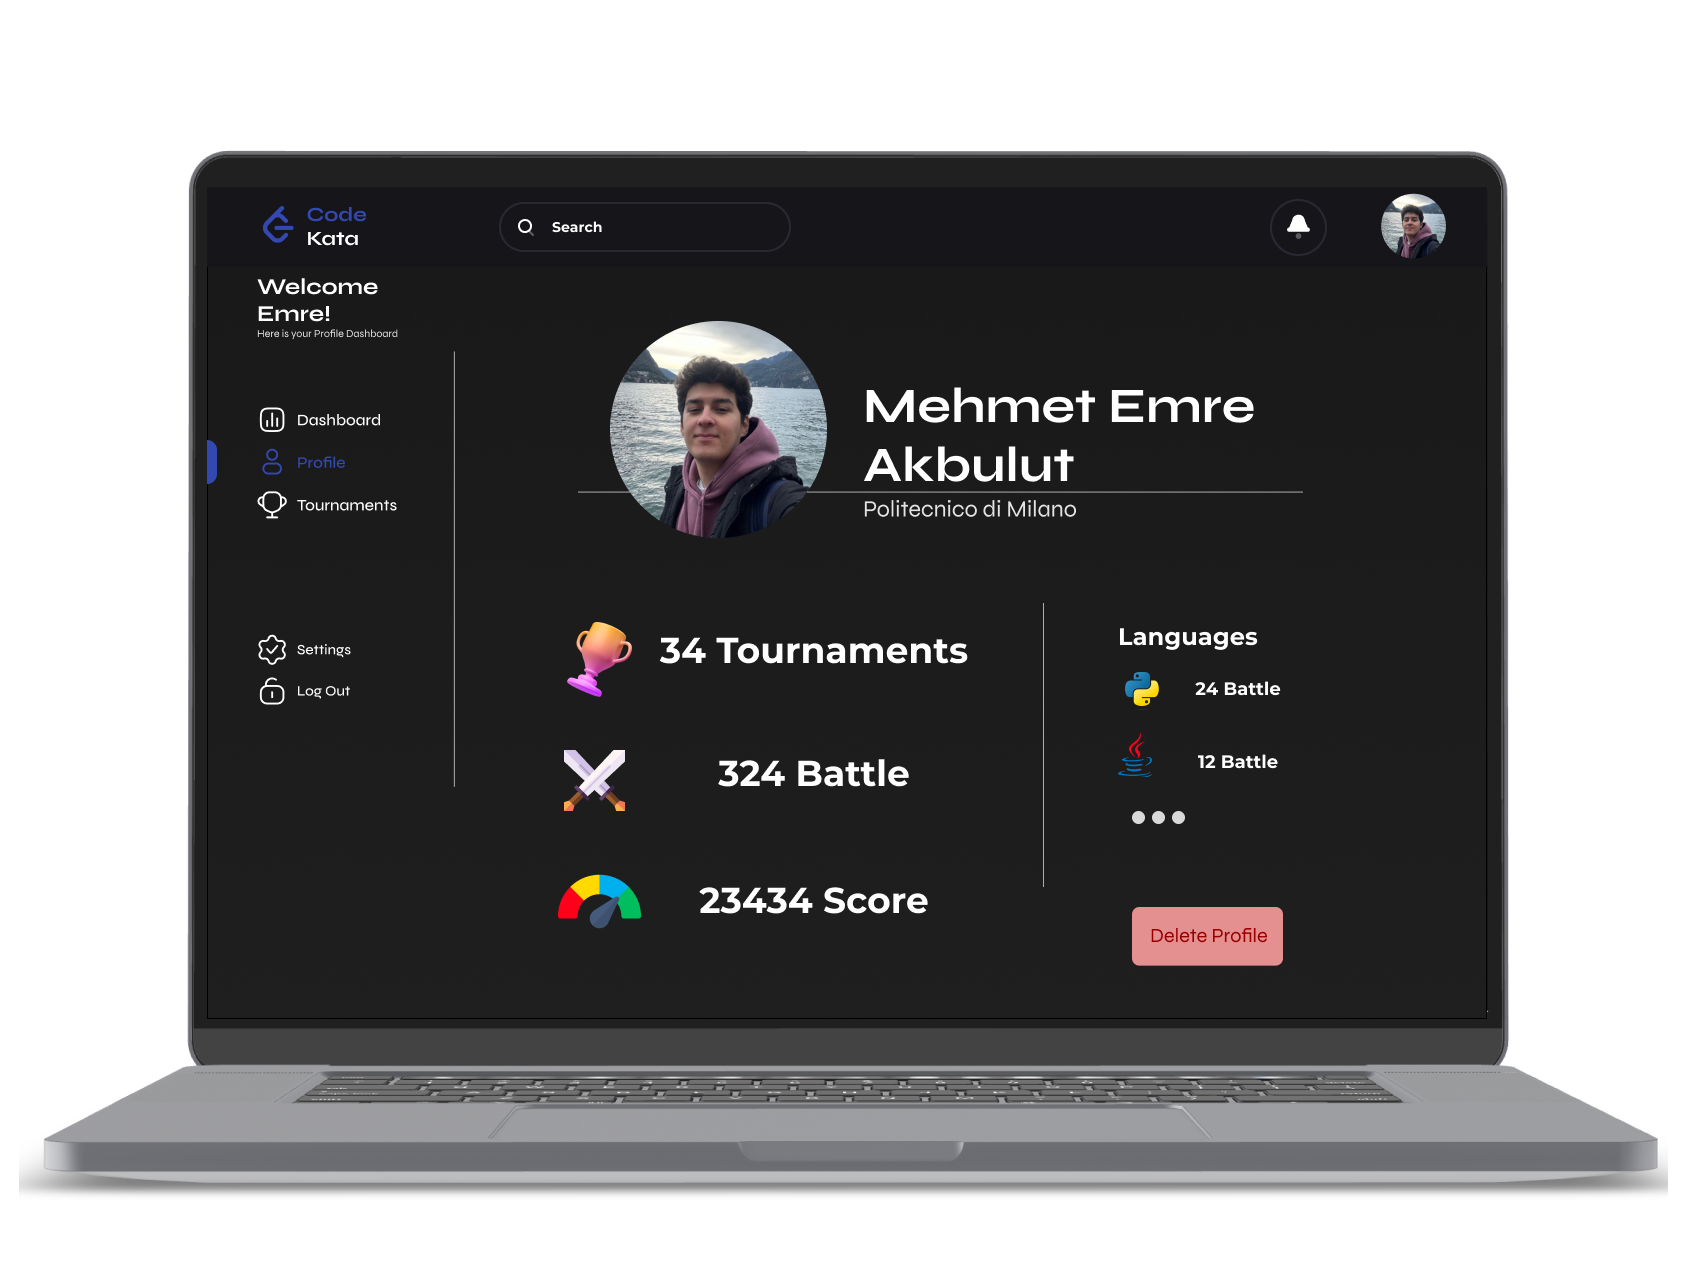
\includegraphics[scale=0.13]{Images/ui-ux/student_profile_settings/student_profile.png}
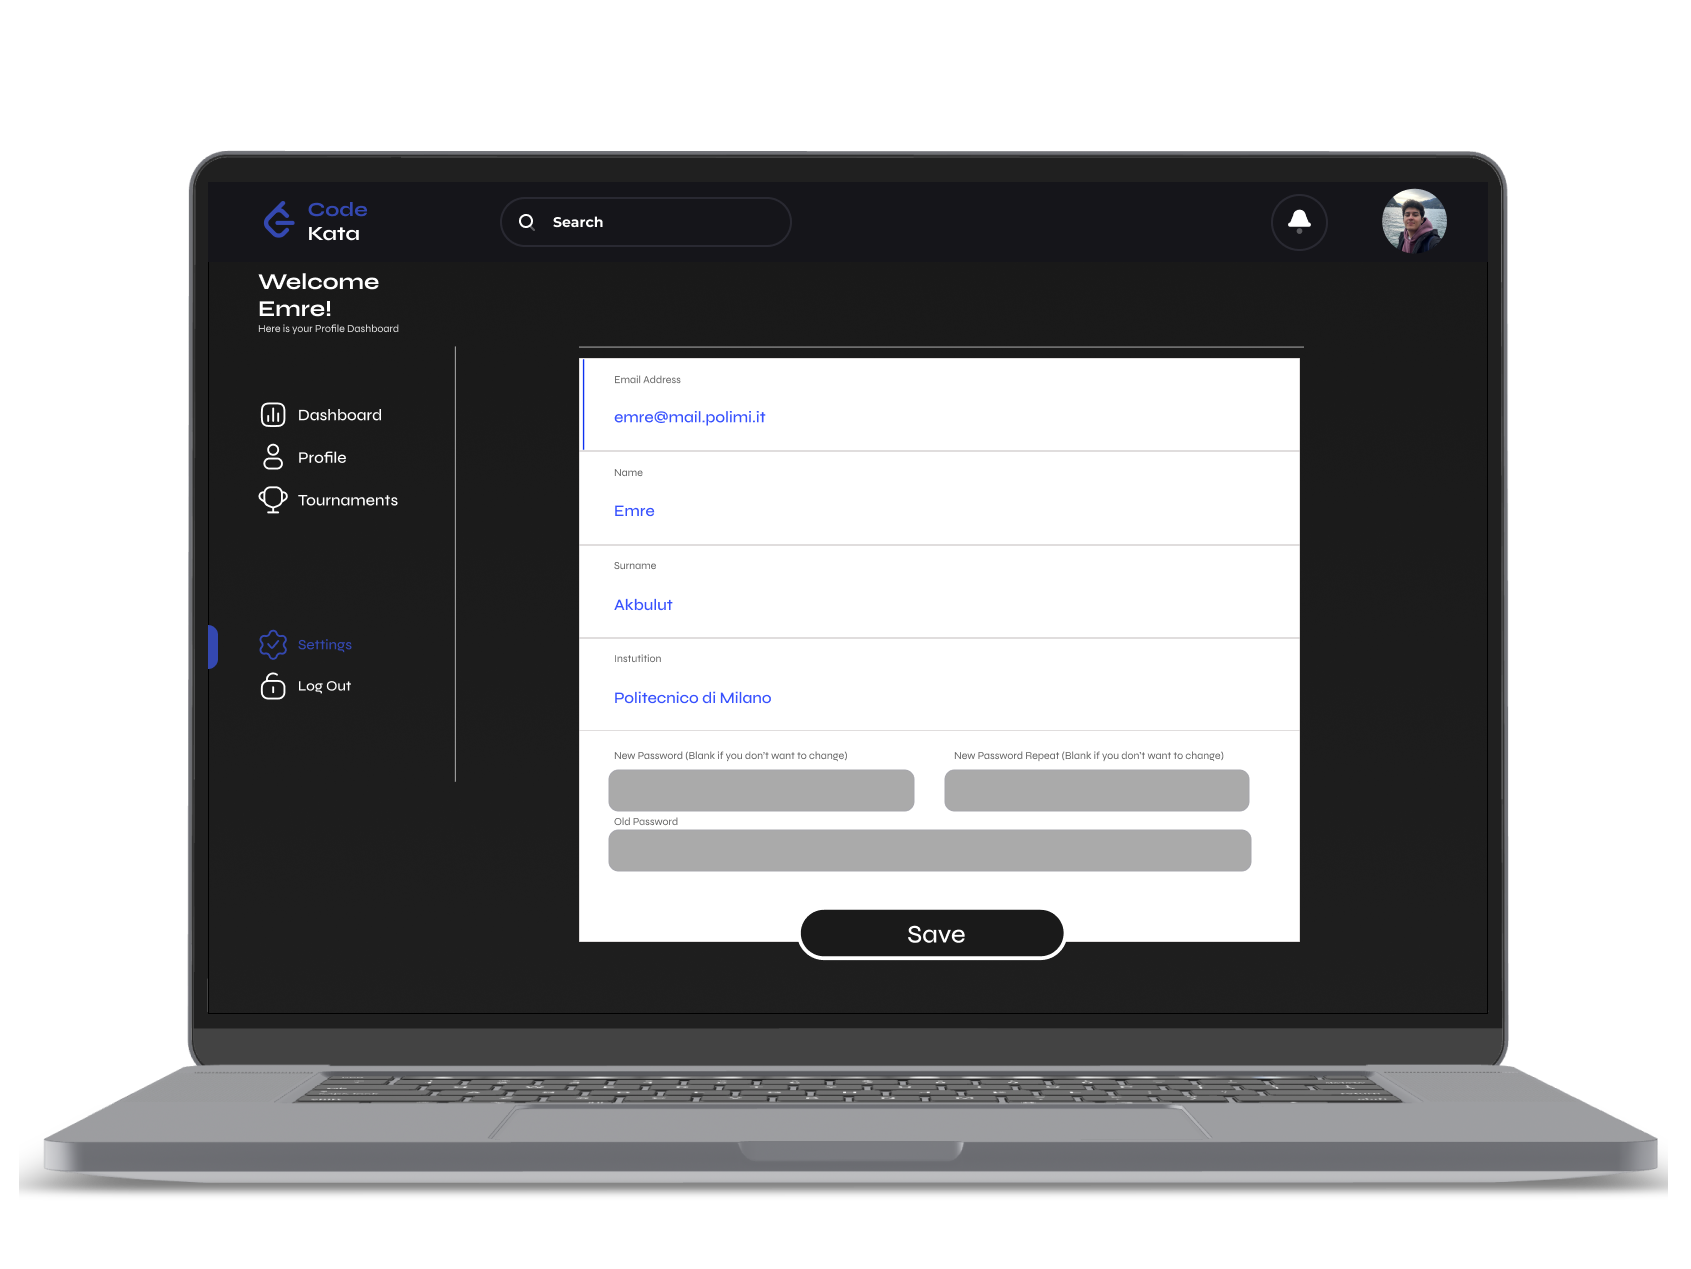
\includegraphics[scale=0.13]{Images/ui-ux/student_profile_settings/student_settings.png}
        (h) Profile and Settings for Student
\end{center}
\newpage
\begin{center}
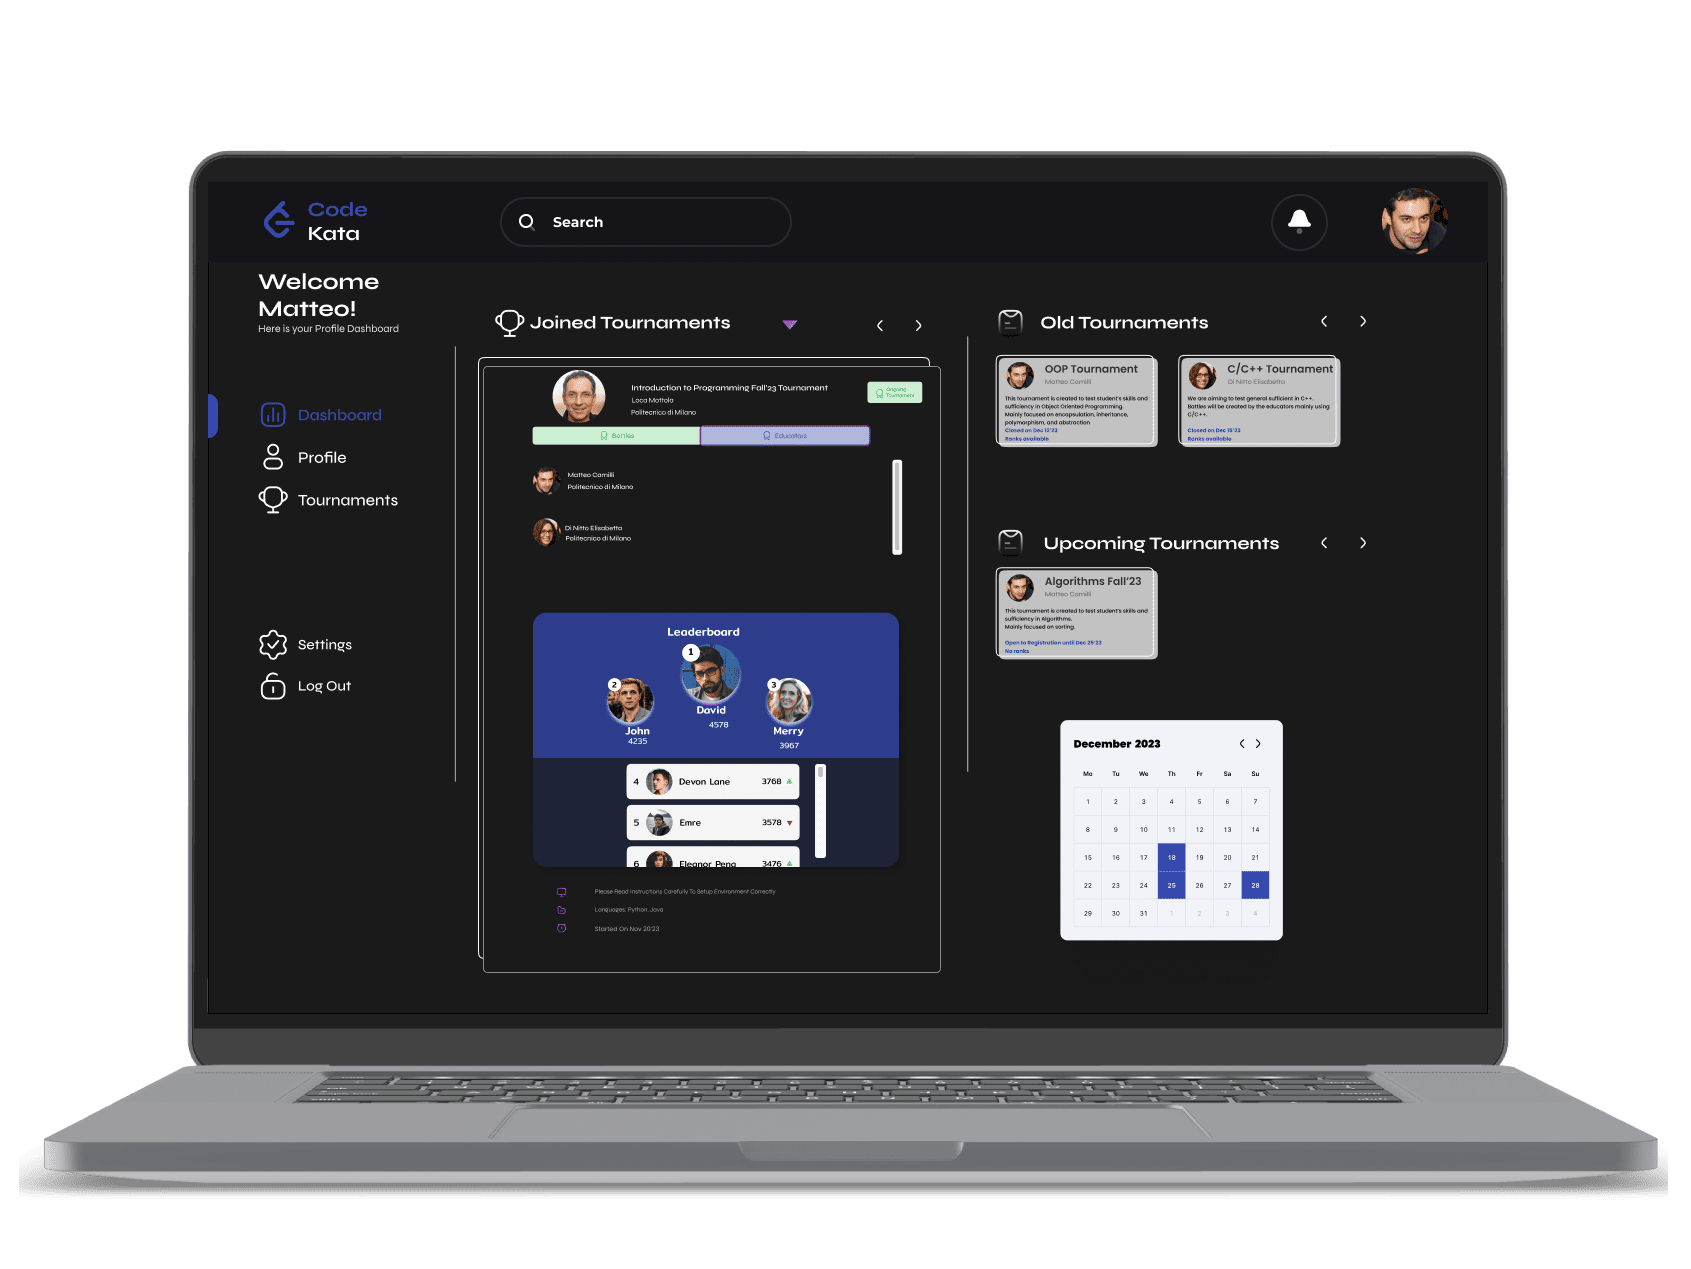
\includegraphics[scale=0.13]{Images/ui-ux/educator_dashboard/educator_dashboard_1.png}
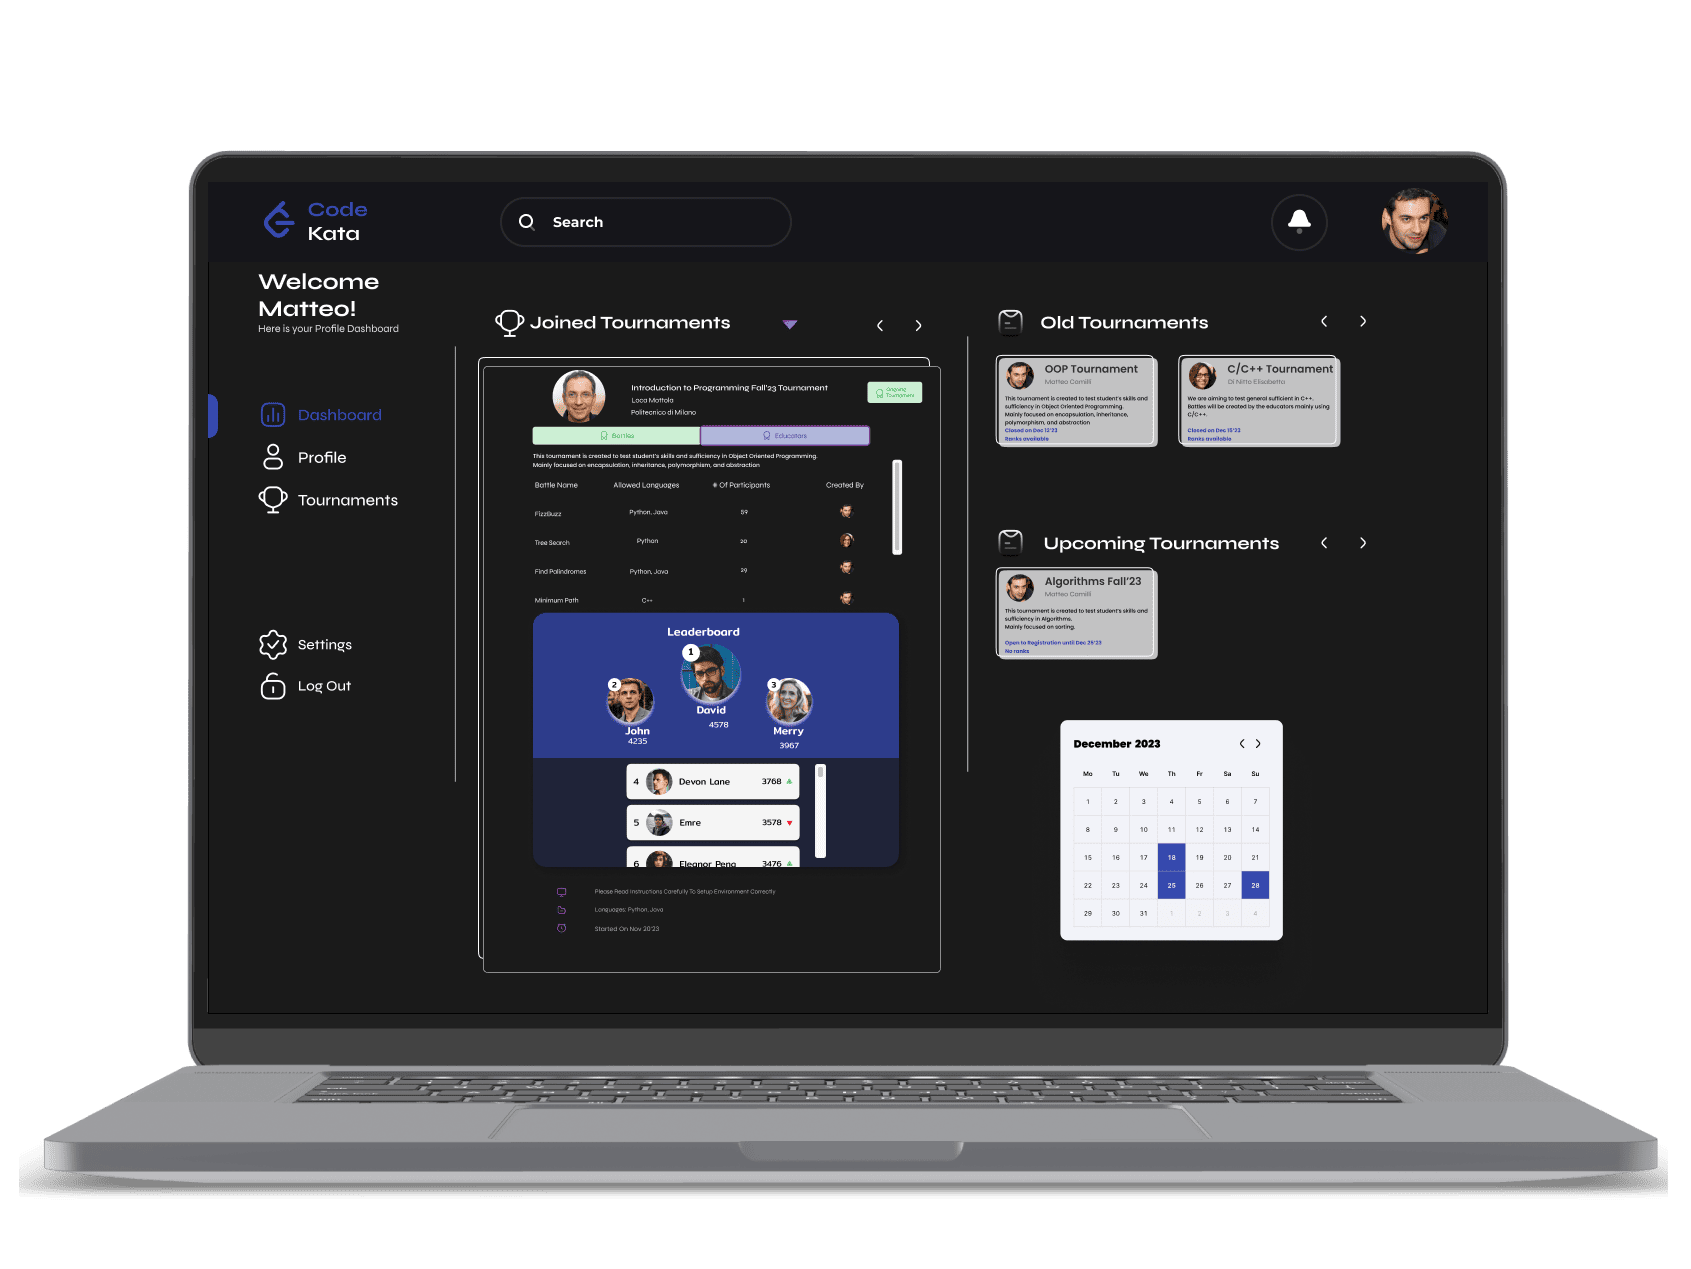
\includegraphics[scale=0.13]{Images/ui-ux/educator_dashboard/educator_dashboard_2.png}
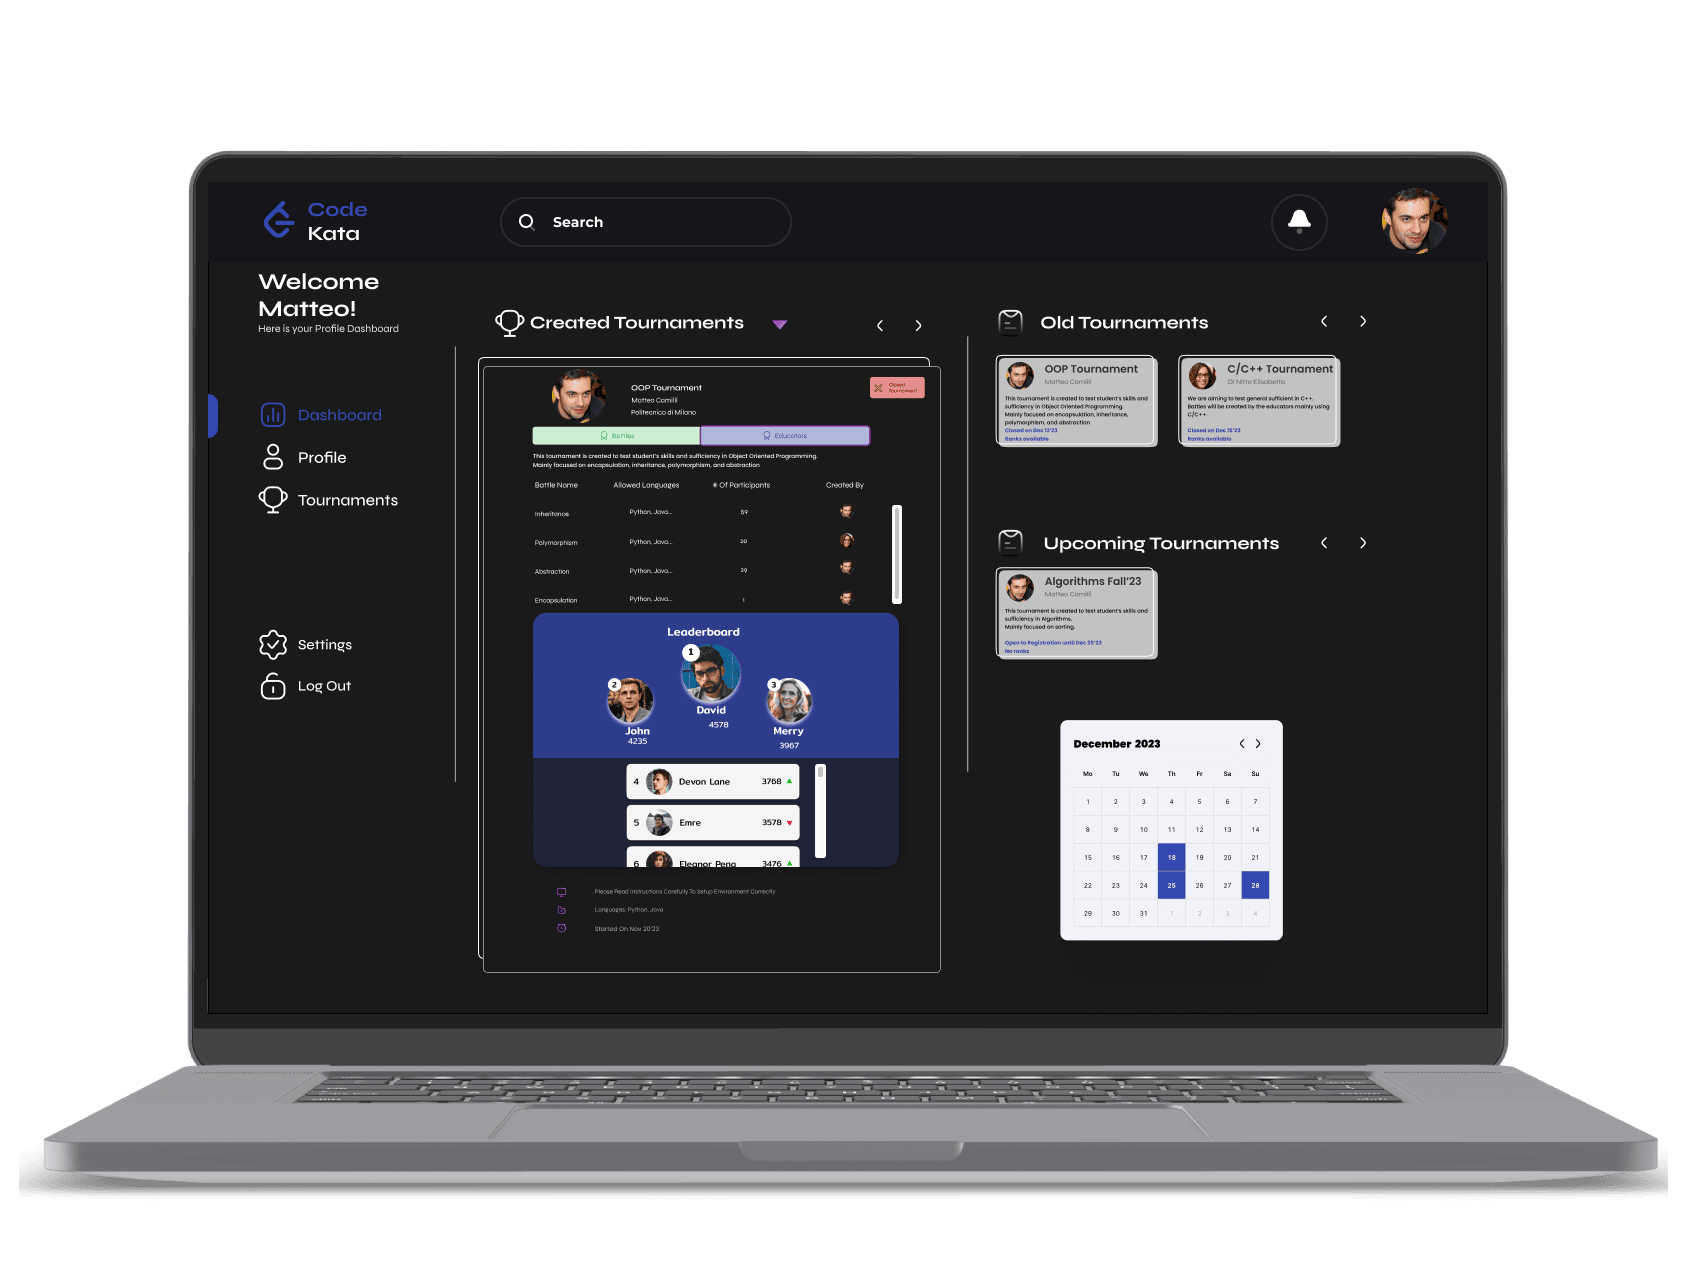
\includegraphics[scale=0.13]{Images/ui-ux/educator_dashboard/educator_dashboard_3.png}
\\ (i) Educator Dashboard
\end{center}
\begin{center}
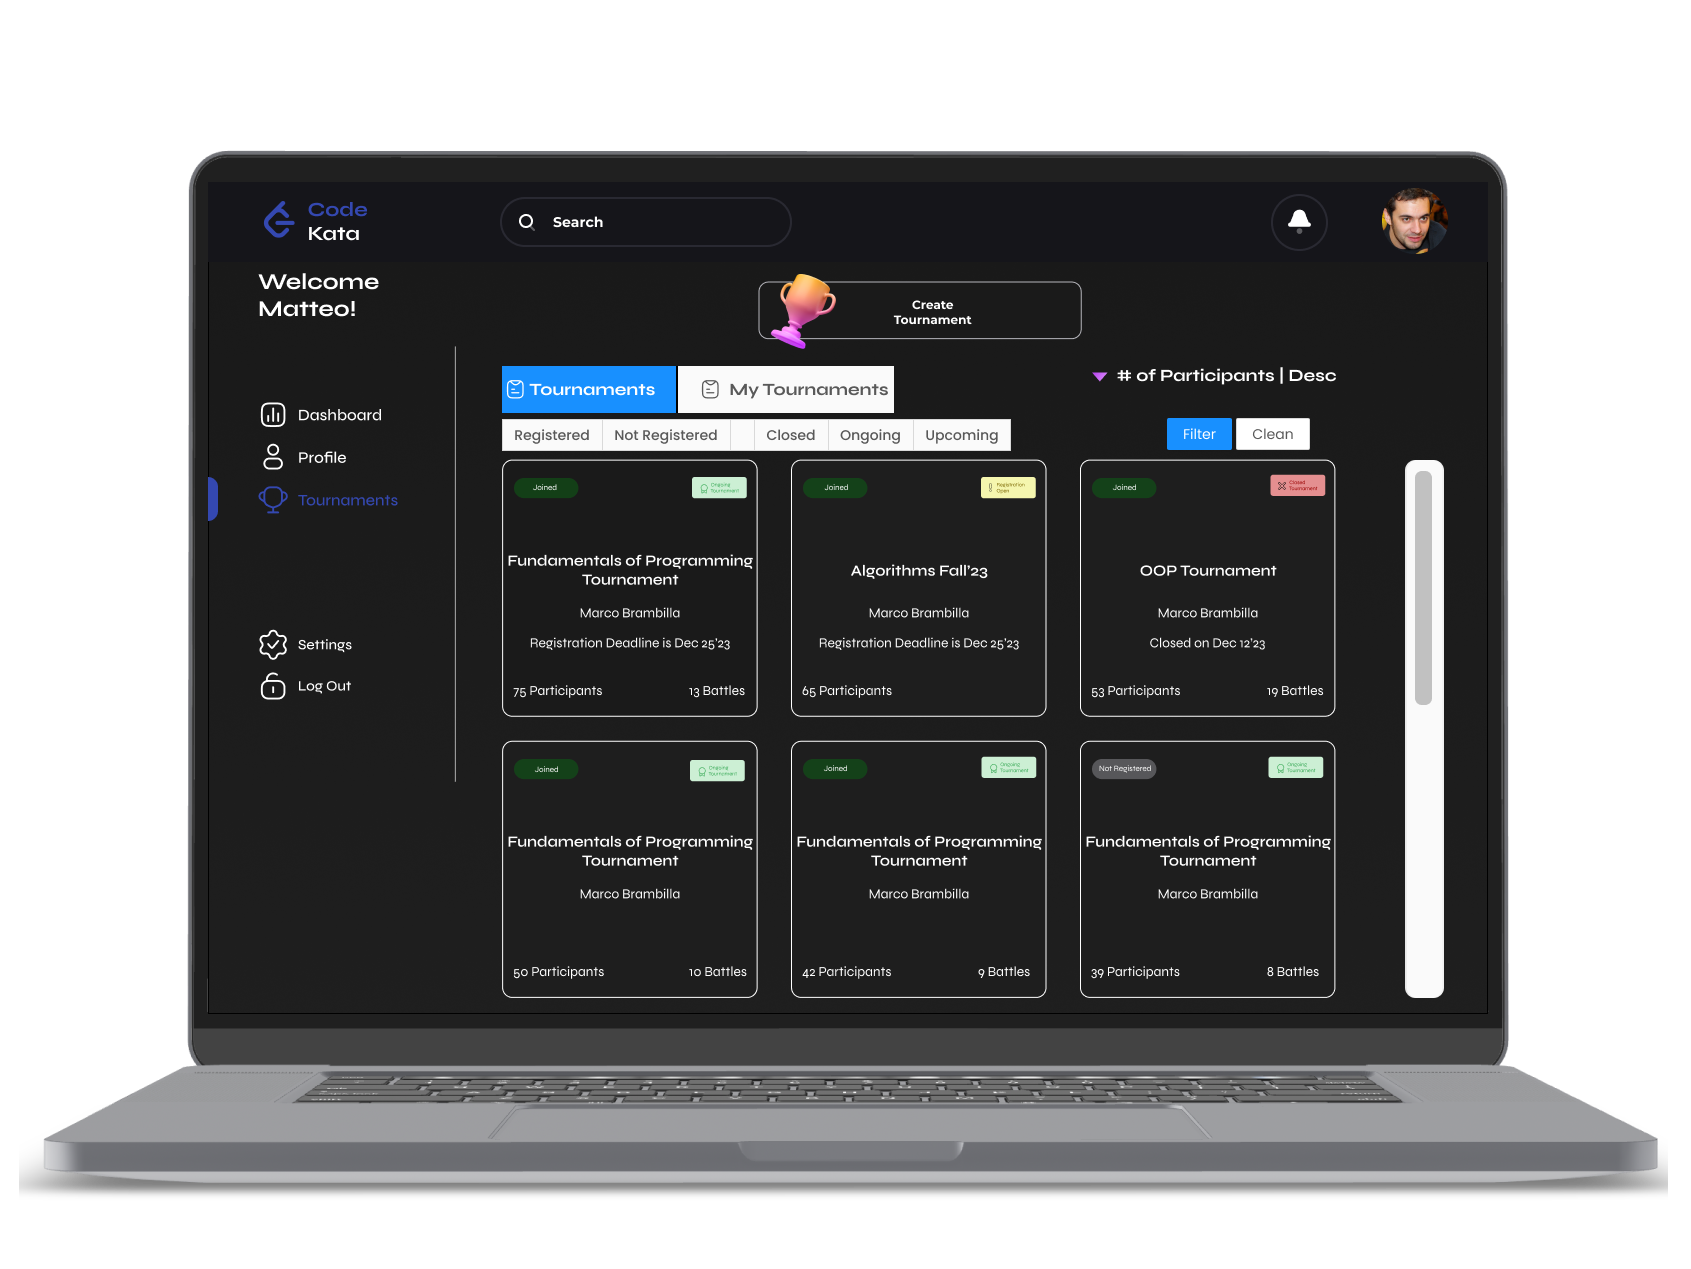
\includegraphics[scale=0.13]{Images/ui-ux/educator_tournaments/educator_tournaments_1.png}
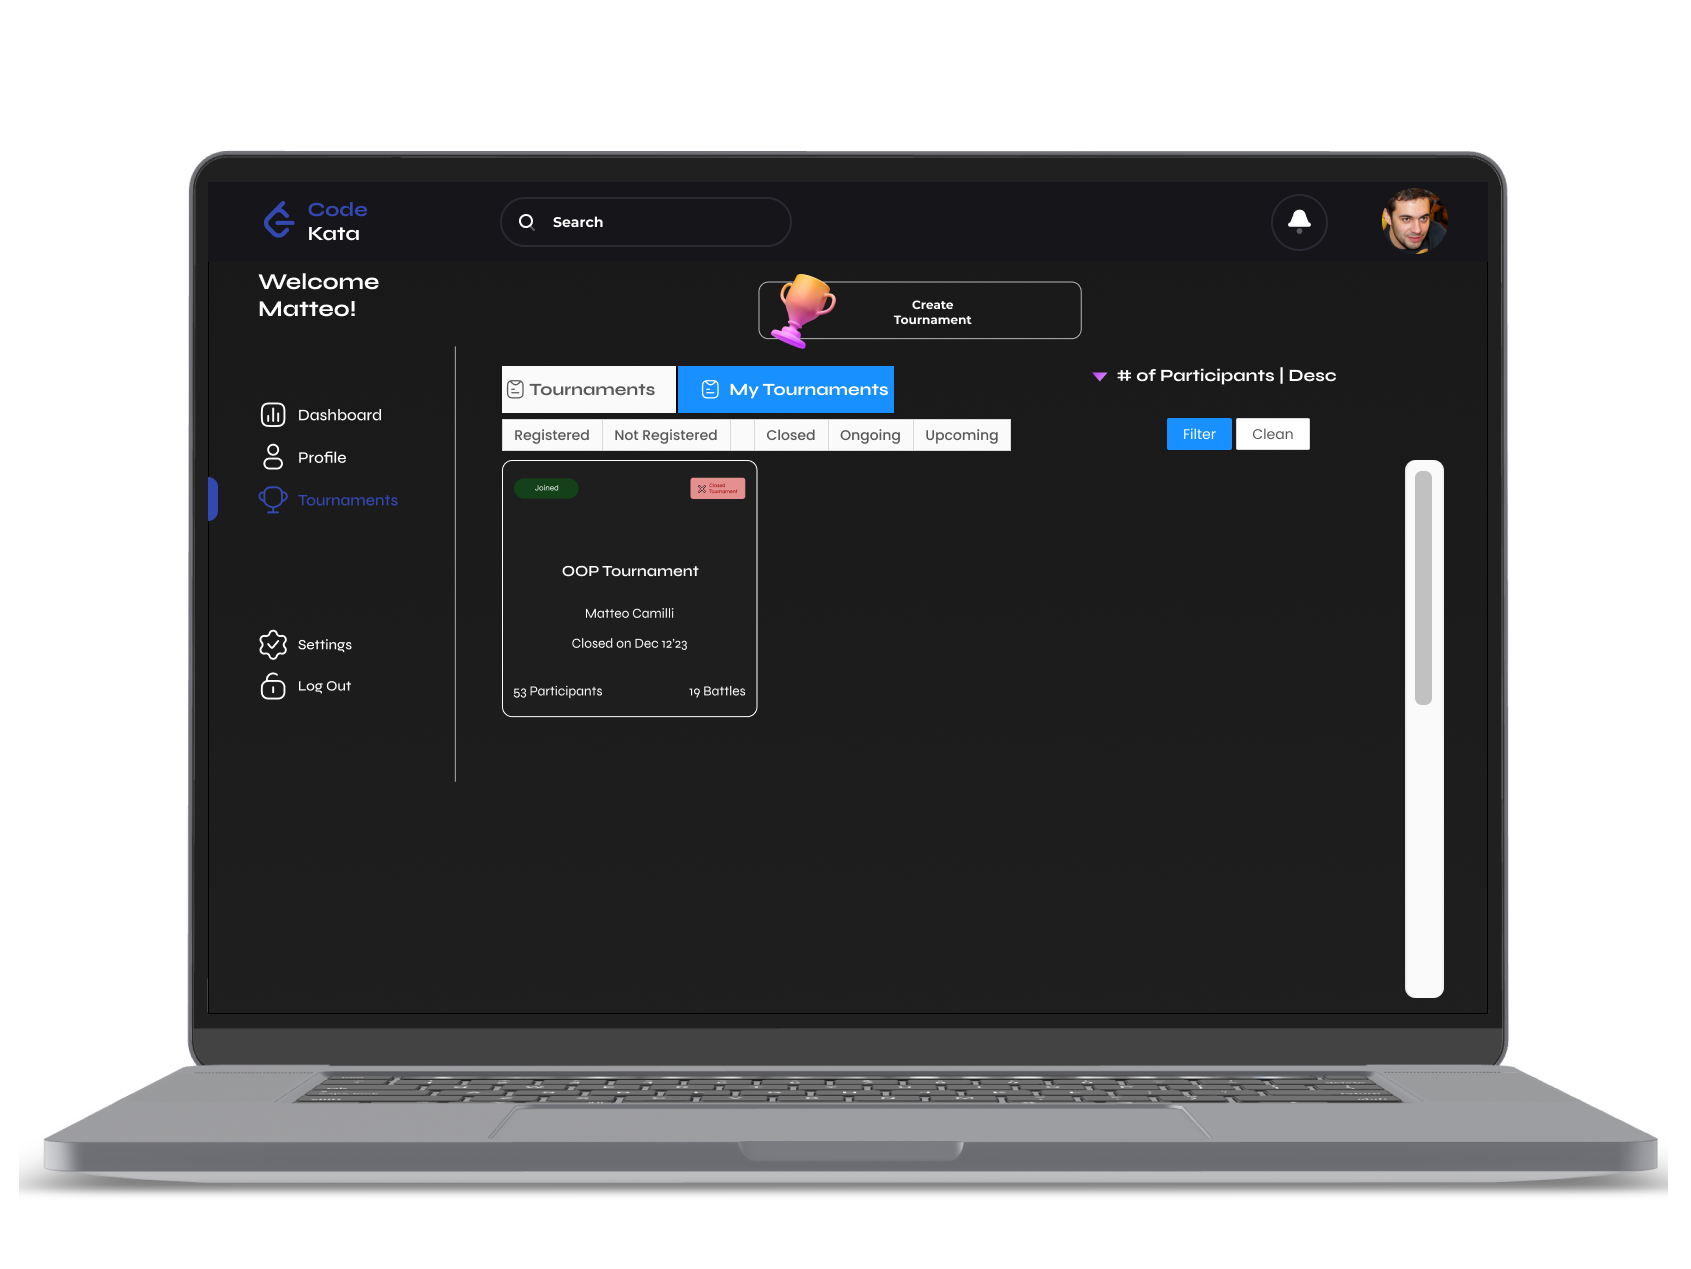
\includegraphics[scale=0.13]{Images/ui-ux/educator_tournaments/educator_tournaments_2.png}
        (j) Educator Tournaments
\end{center}
\begin{center}
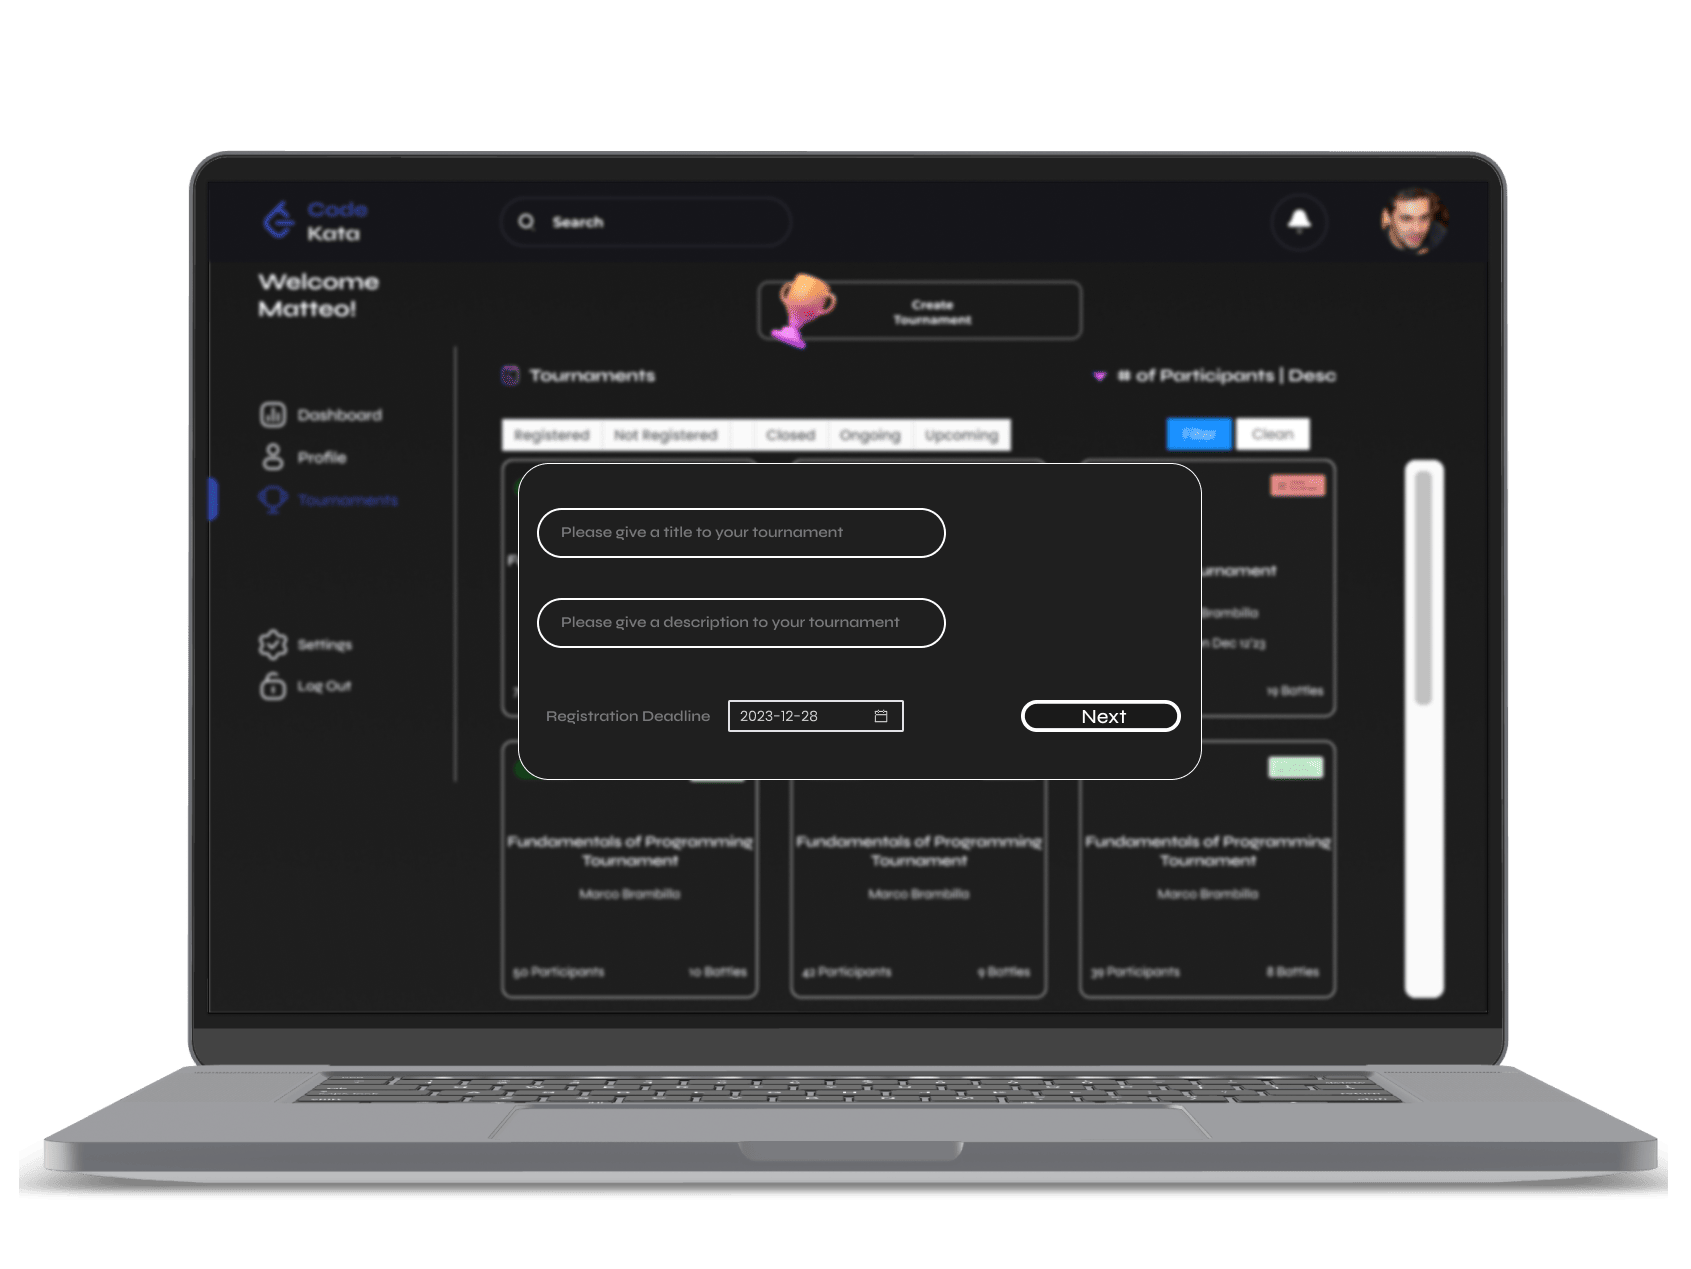
\includegraphics[scale=0.13]{Images/ui-ux/educator_create_tournament/educator_create_tournament_1.png}
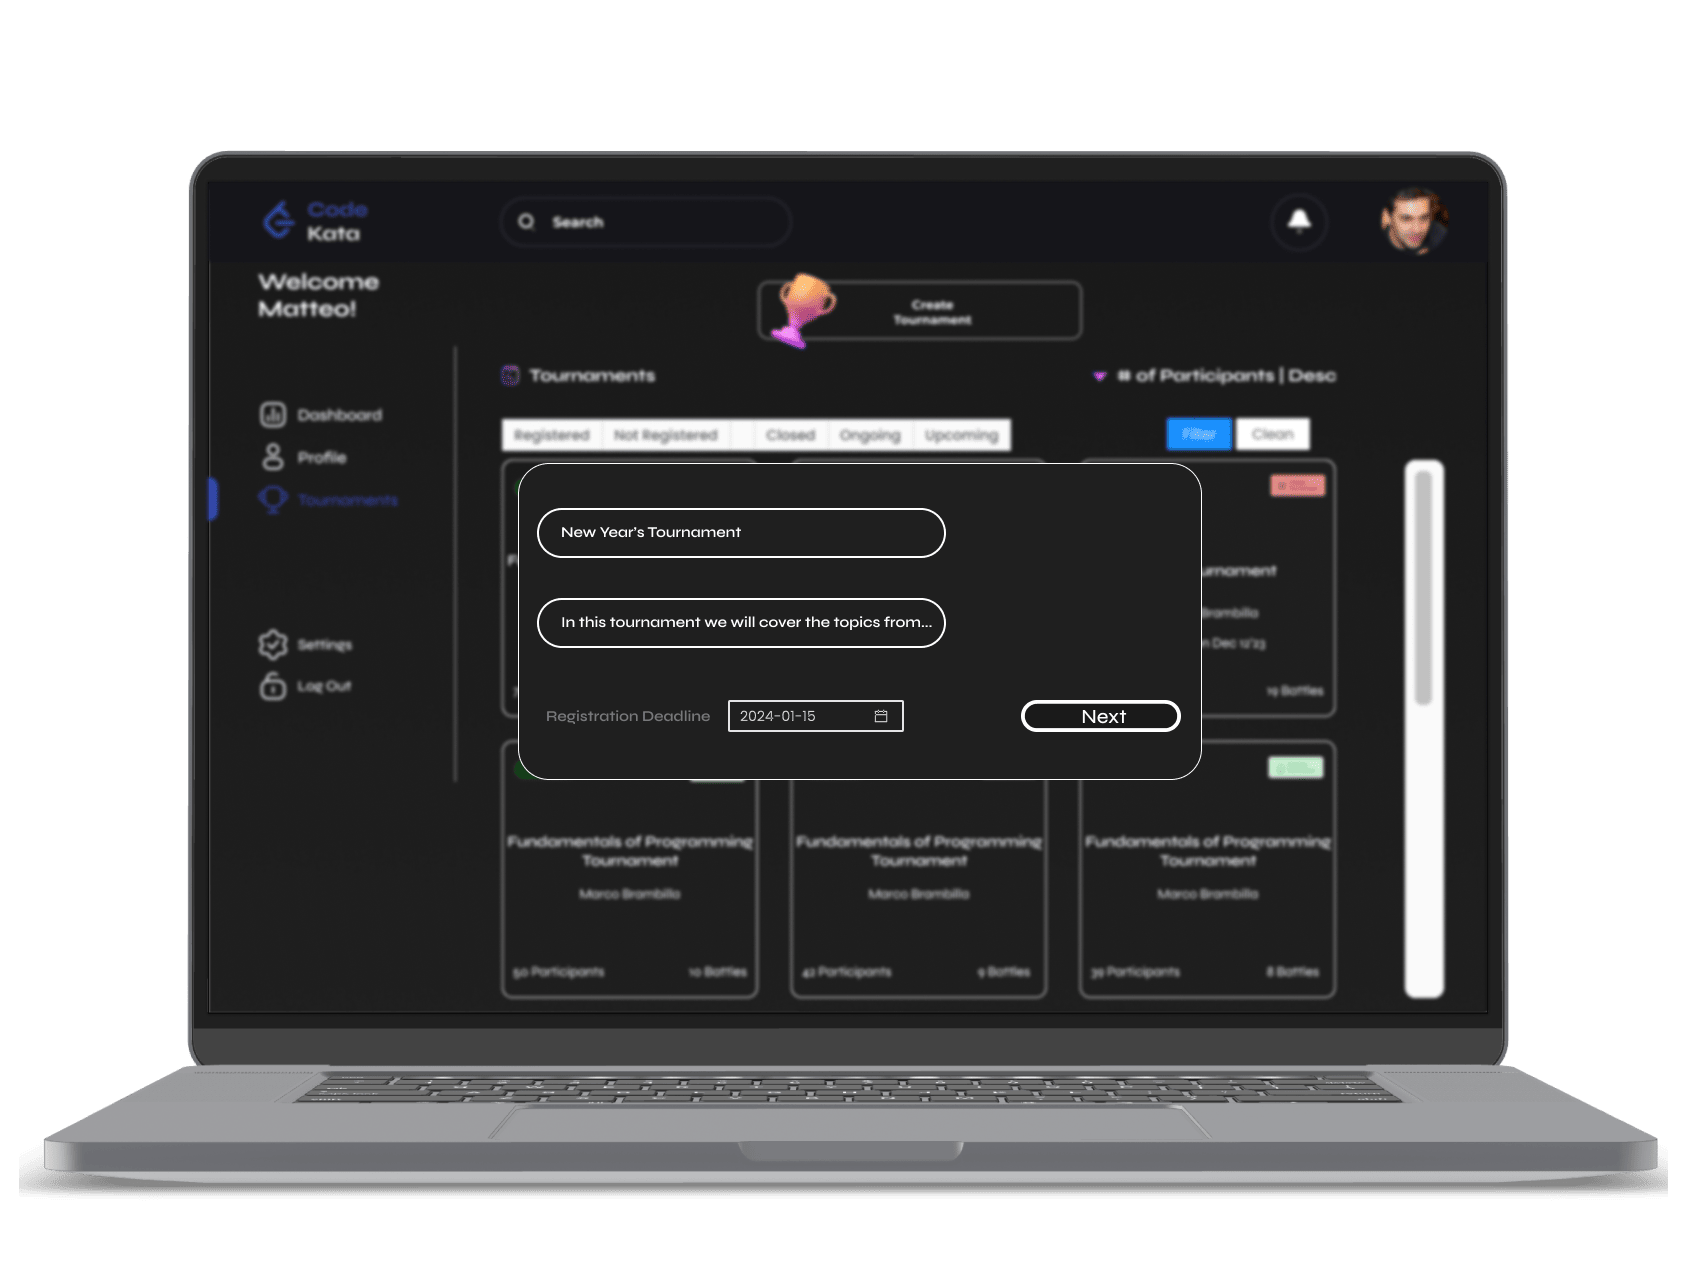
\includegraphics[scale=0.13]{Images/ui-ux/educator_create_tournament/educator_create_tournament_2.png}
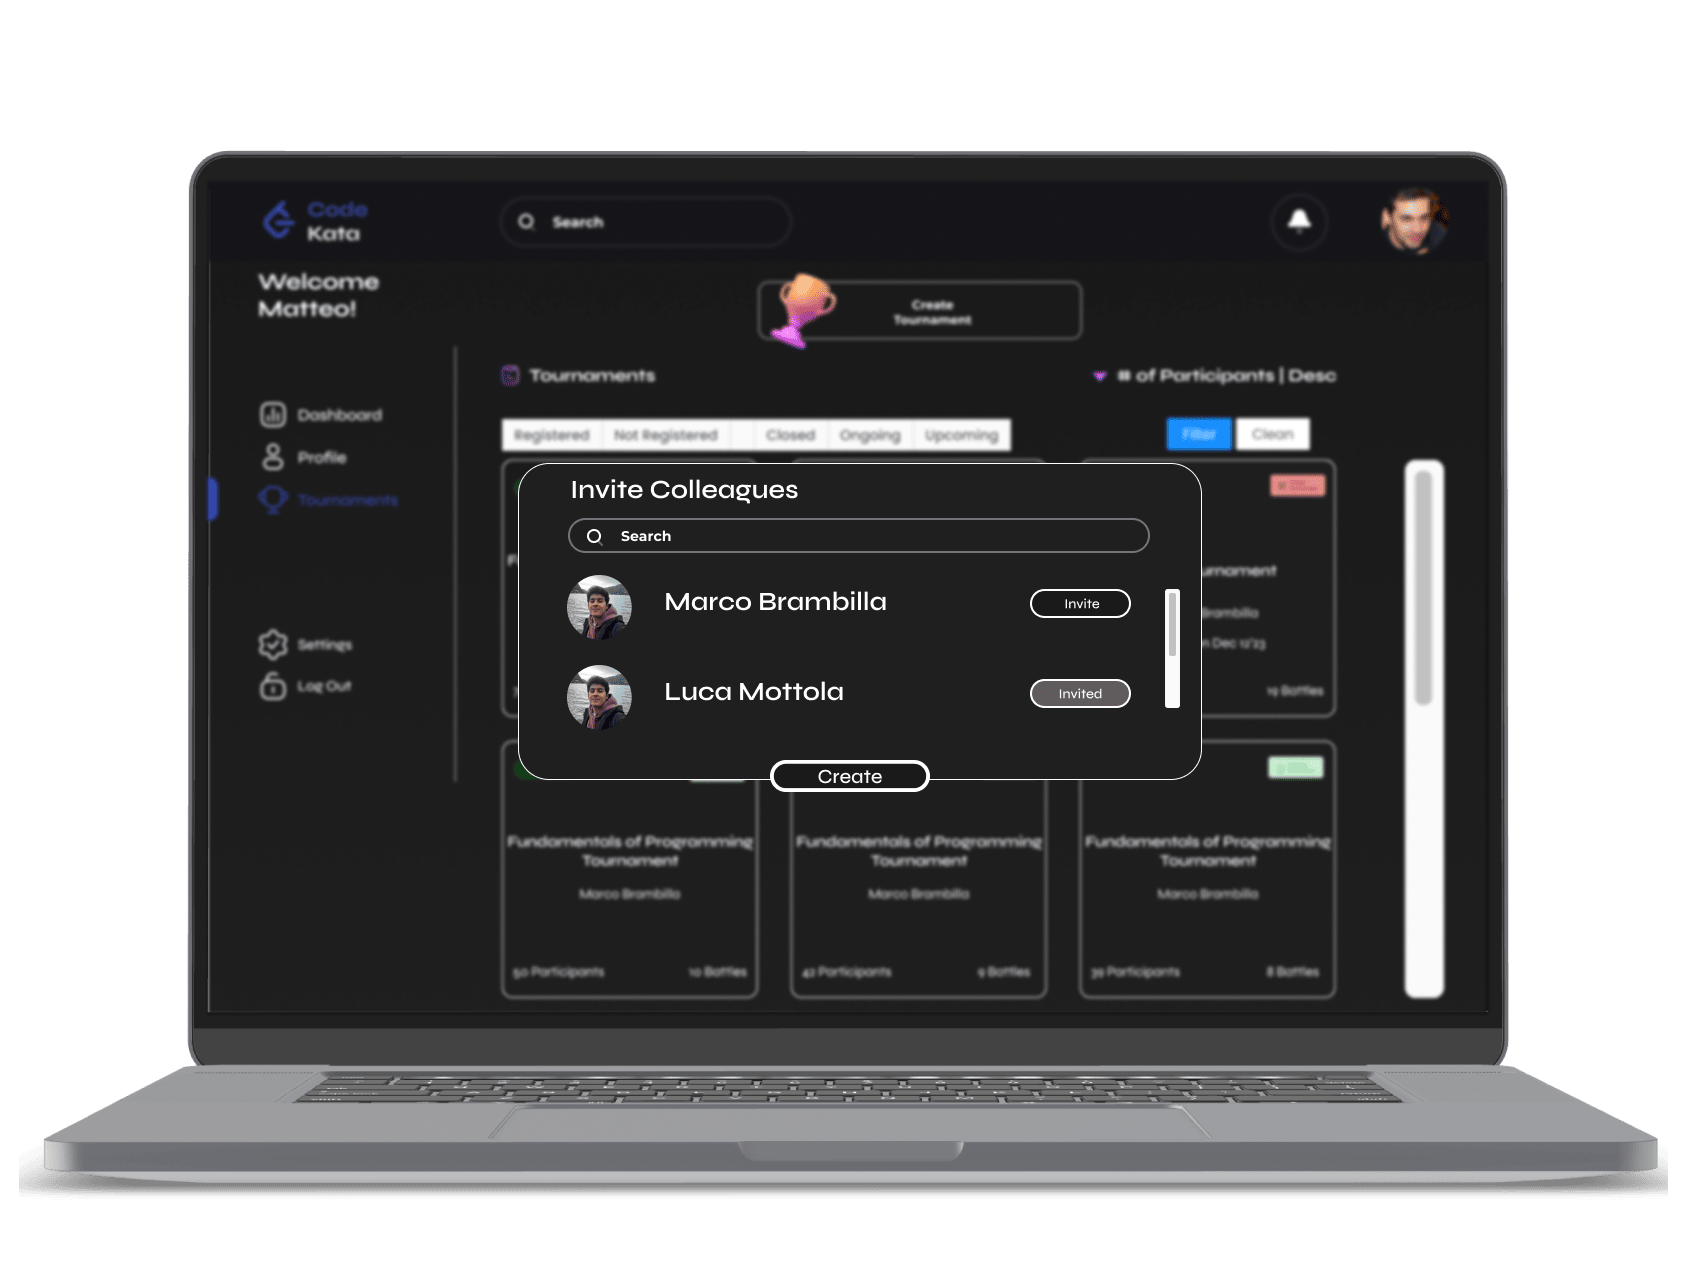
\includegraphics[scale=0.13]{Images/ui-ux/educator_create_tournament/educator_create_tournament_3.png}
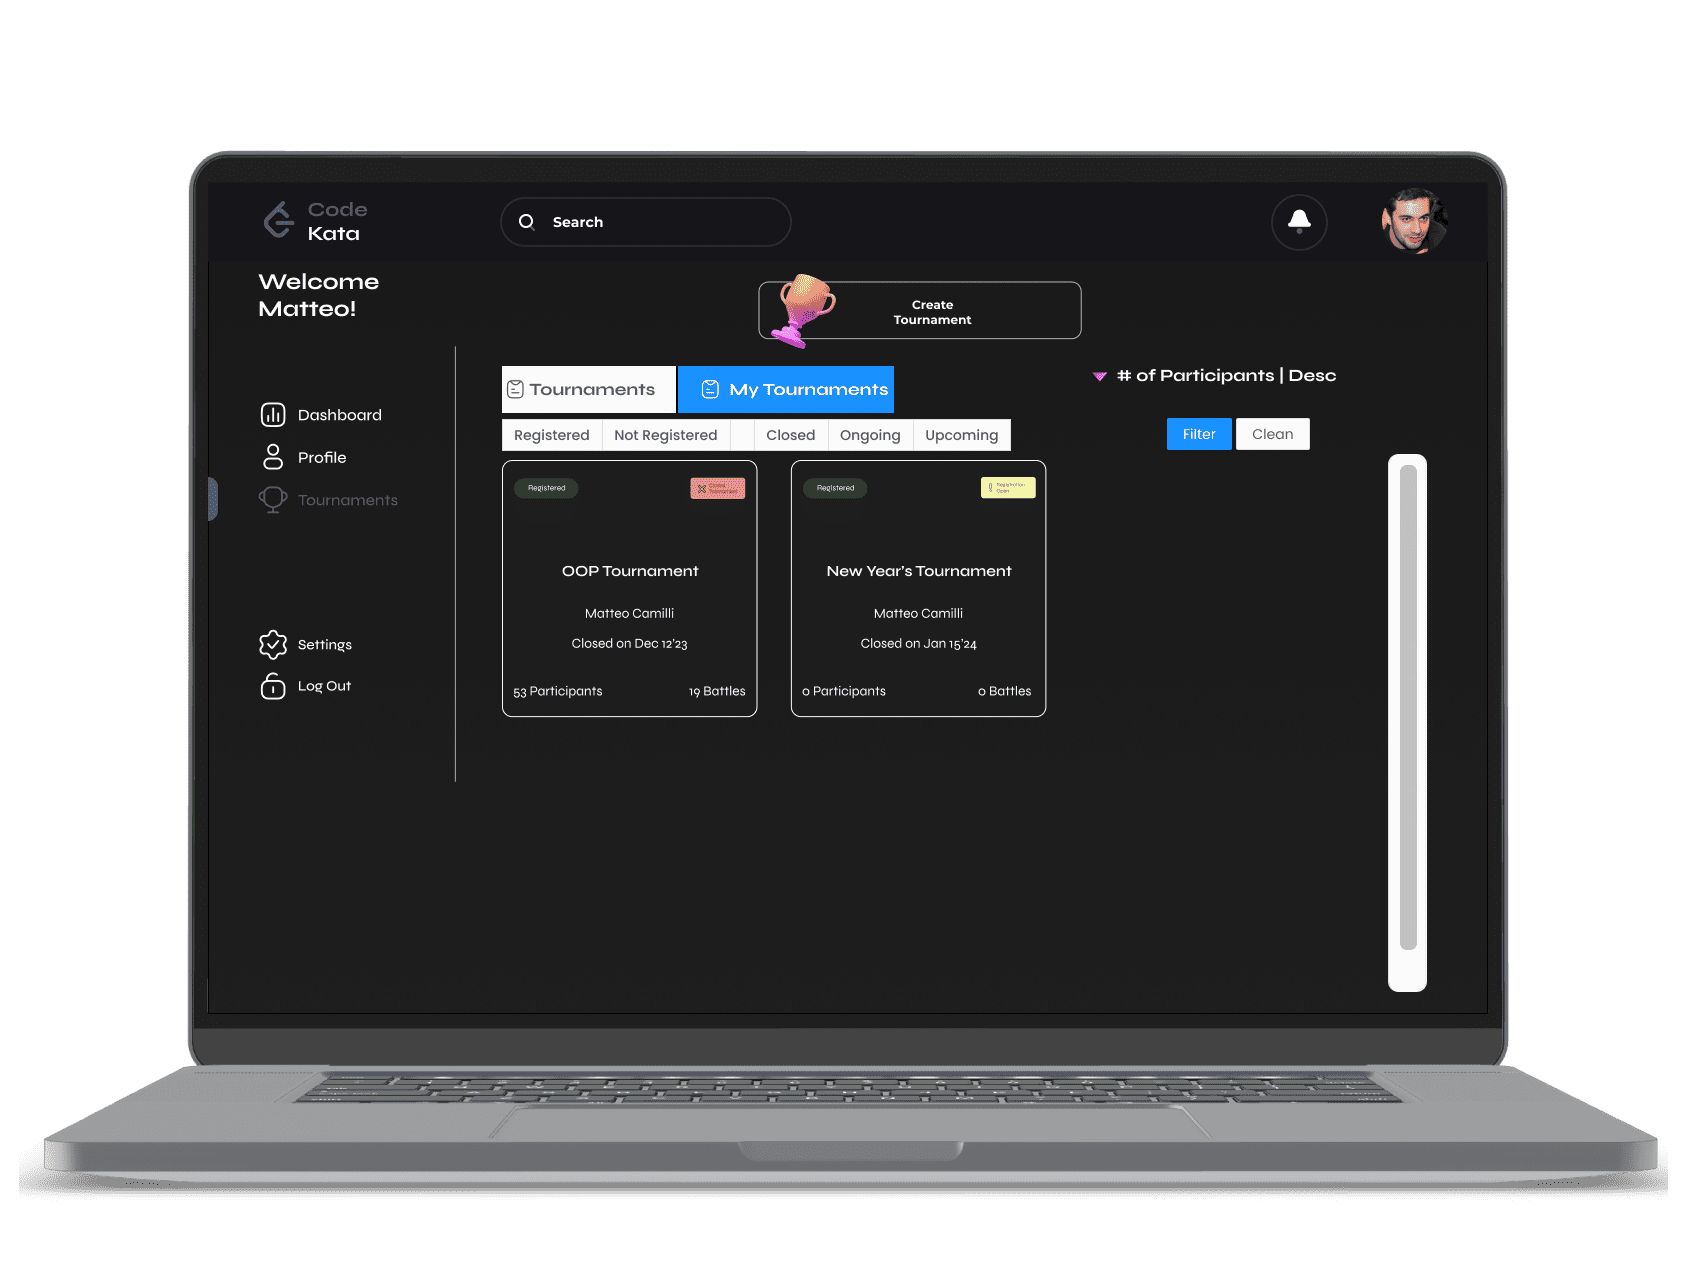
\includegraphics[scale=0.13]{Images/ui-ux/educator_create_tournament/educator_create_tournament_4.png}
        (k) Educator Creates Tournament
\end{center}
\newpage
\begin{center}
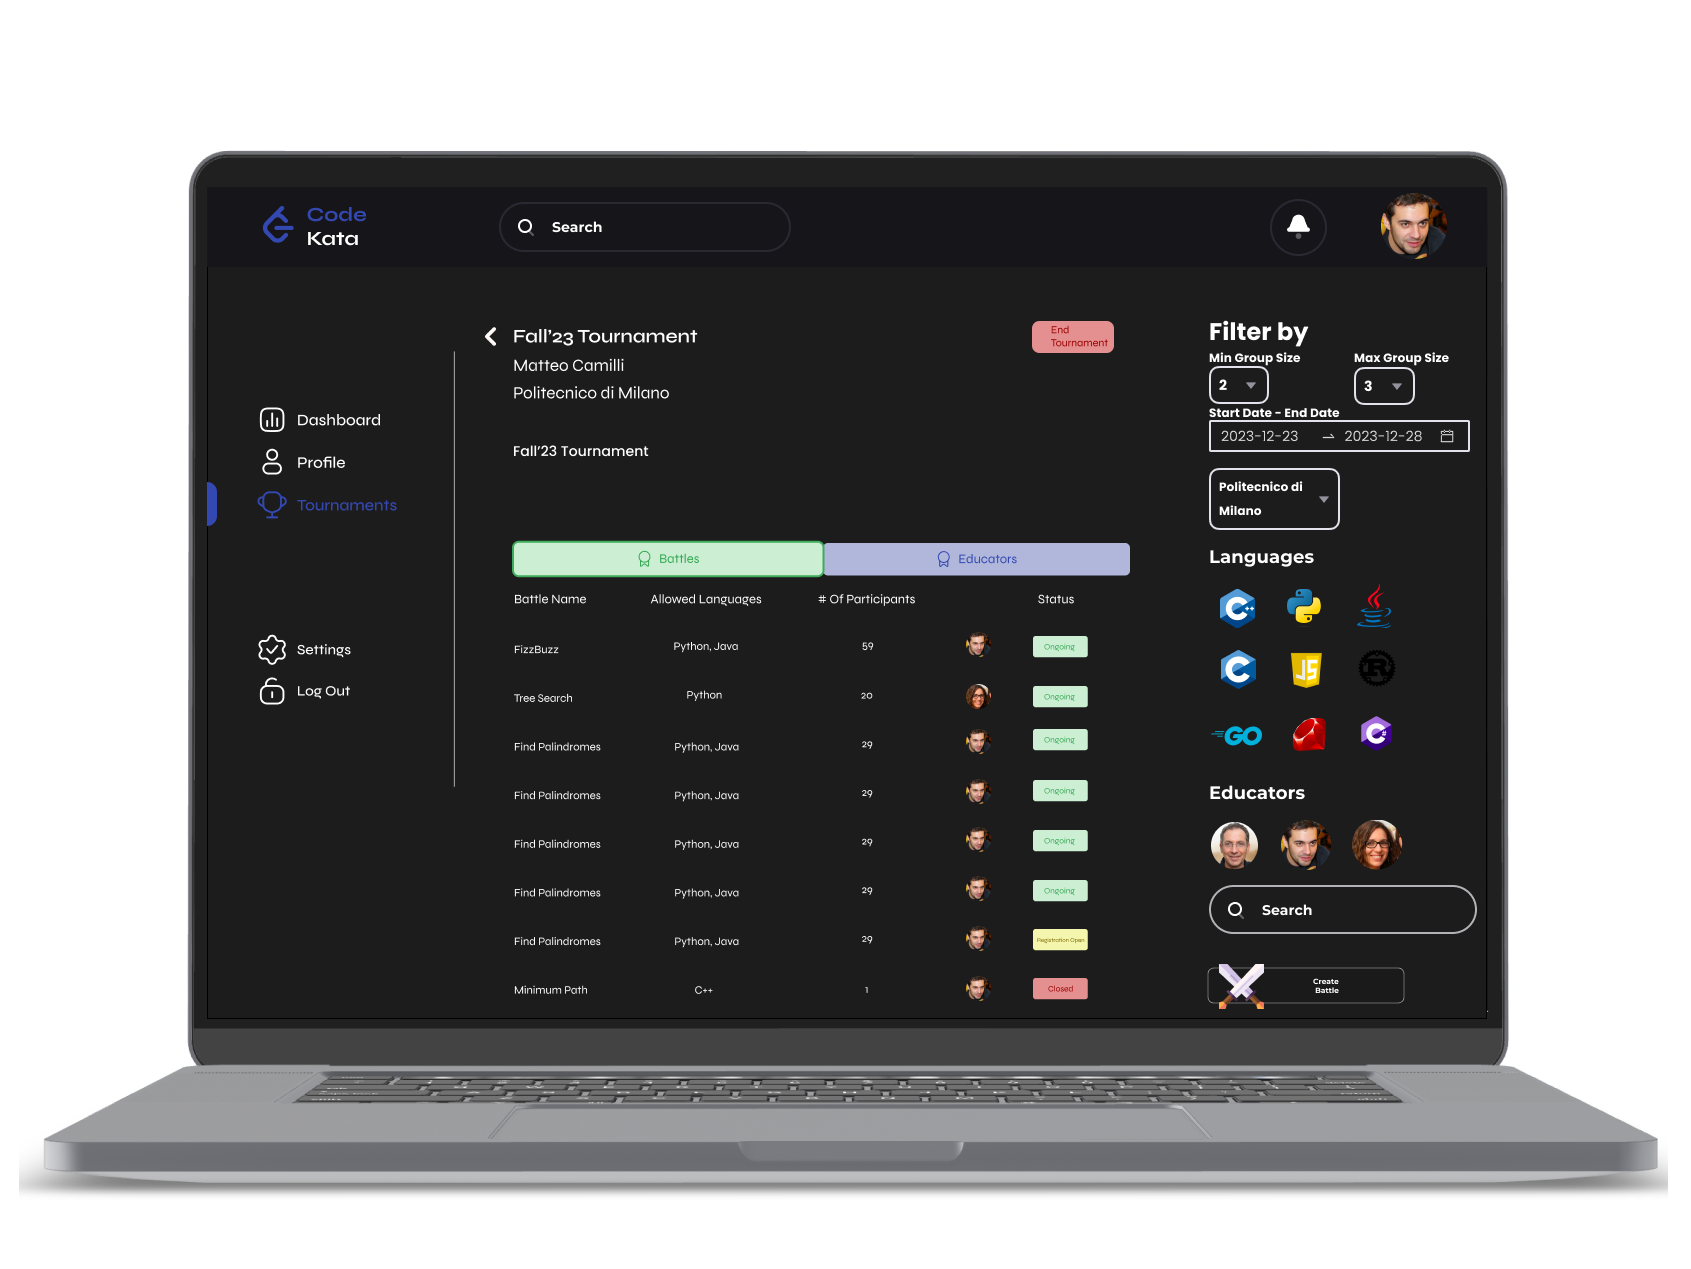
\includegraphics[scale=0.13]{Images/ui-ux/educator_creates_battle/educator_creates_battle_1.png}
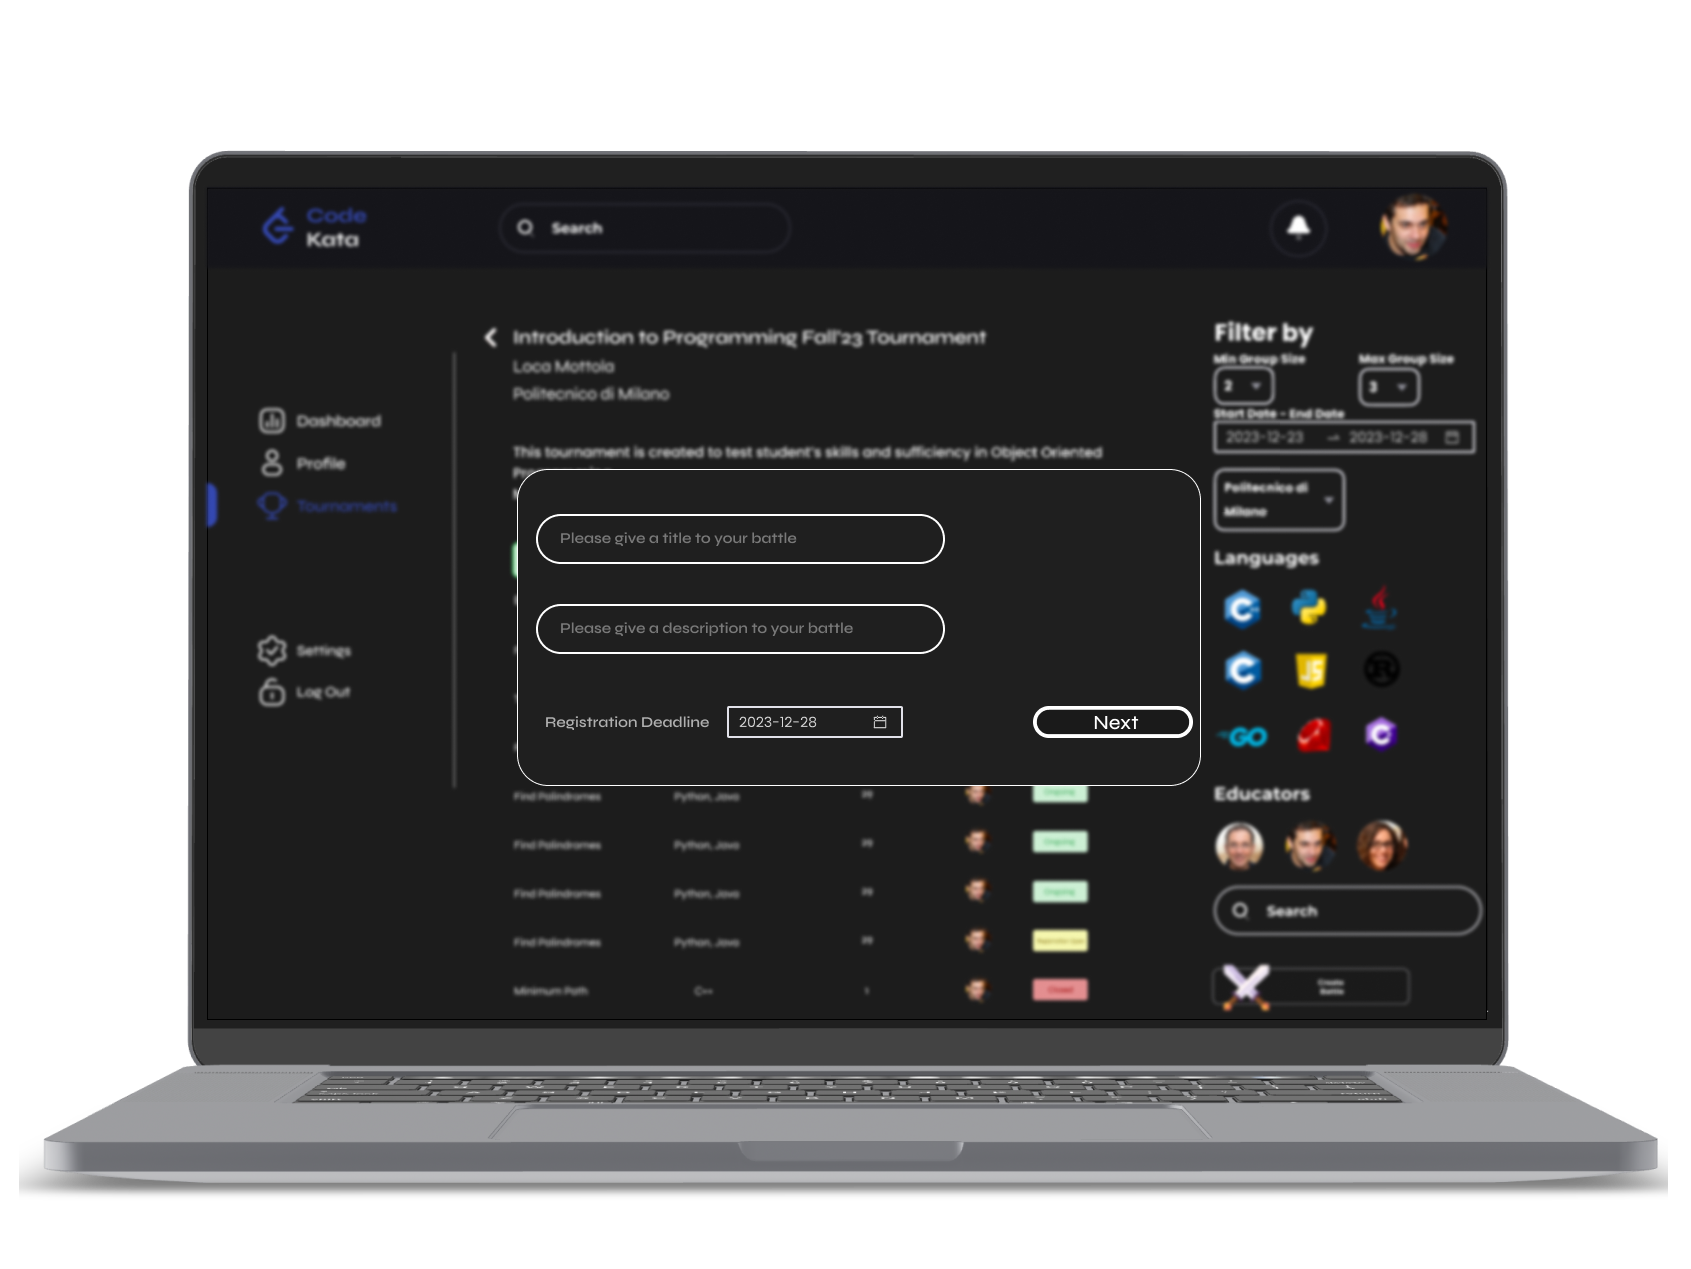
\includegraphics[scale=0.13]{Images/ui-ux/educator_creates_battle/educator_creates_battle_2.png}
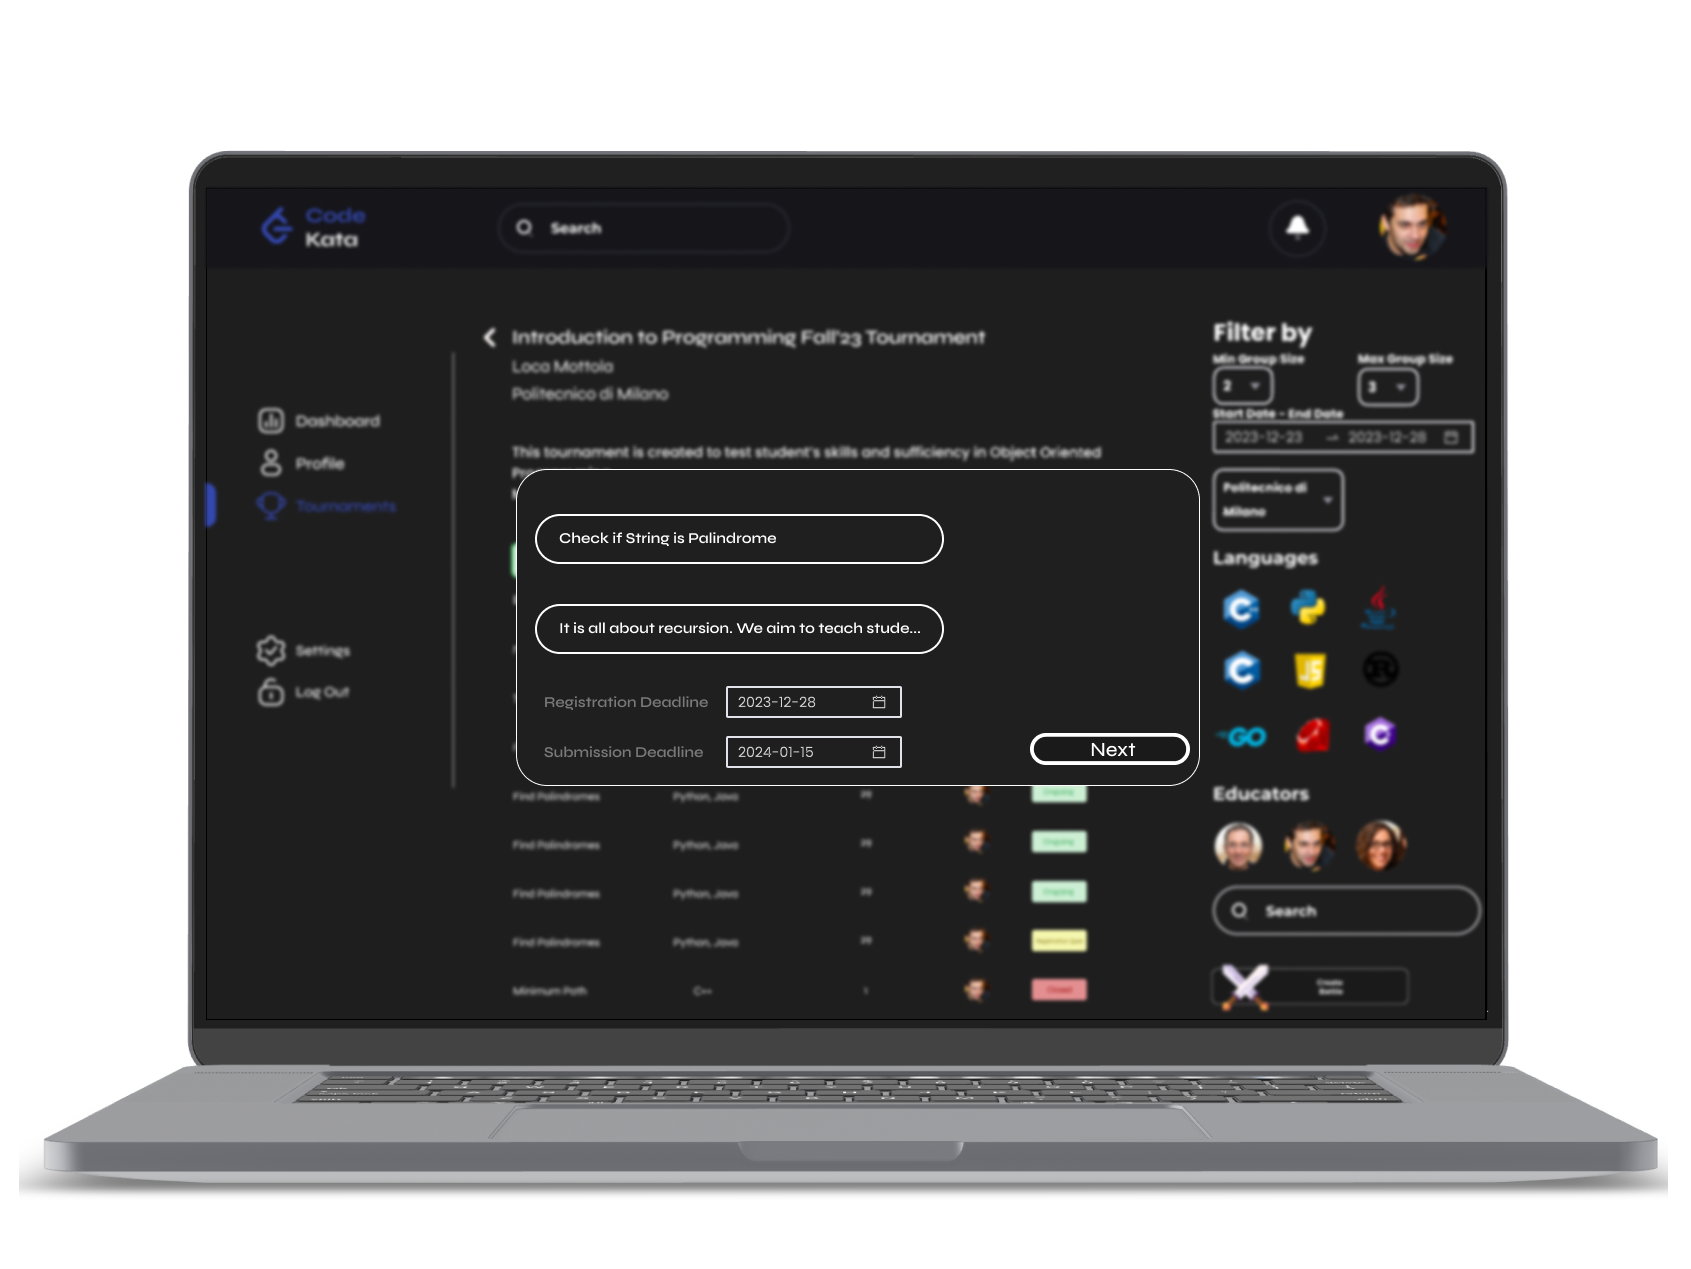
\includegraphics[scale=0.13]{Images/ui-ux/educator_creates_battle/educator_creates_battle_3.png}
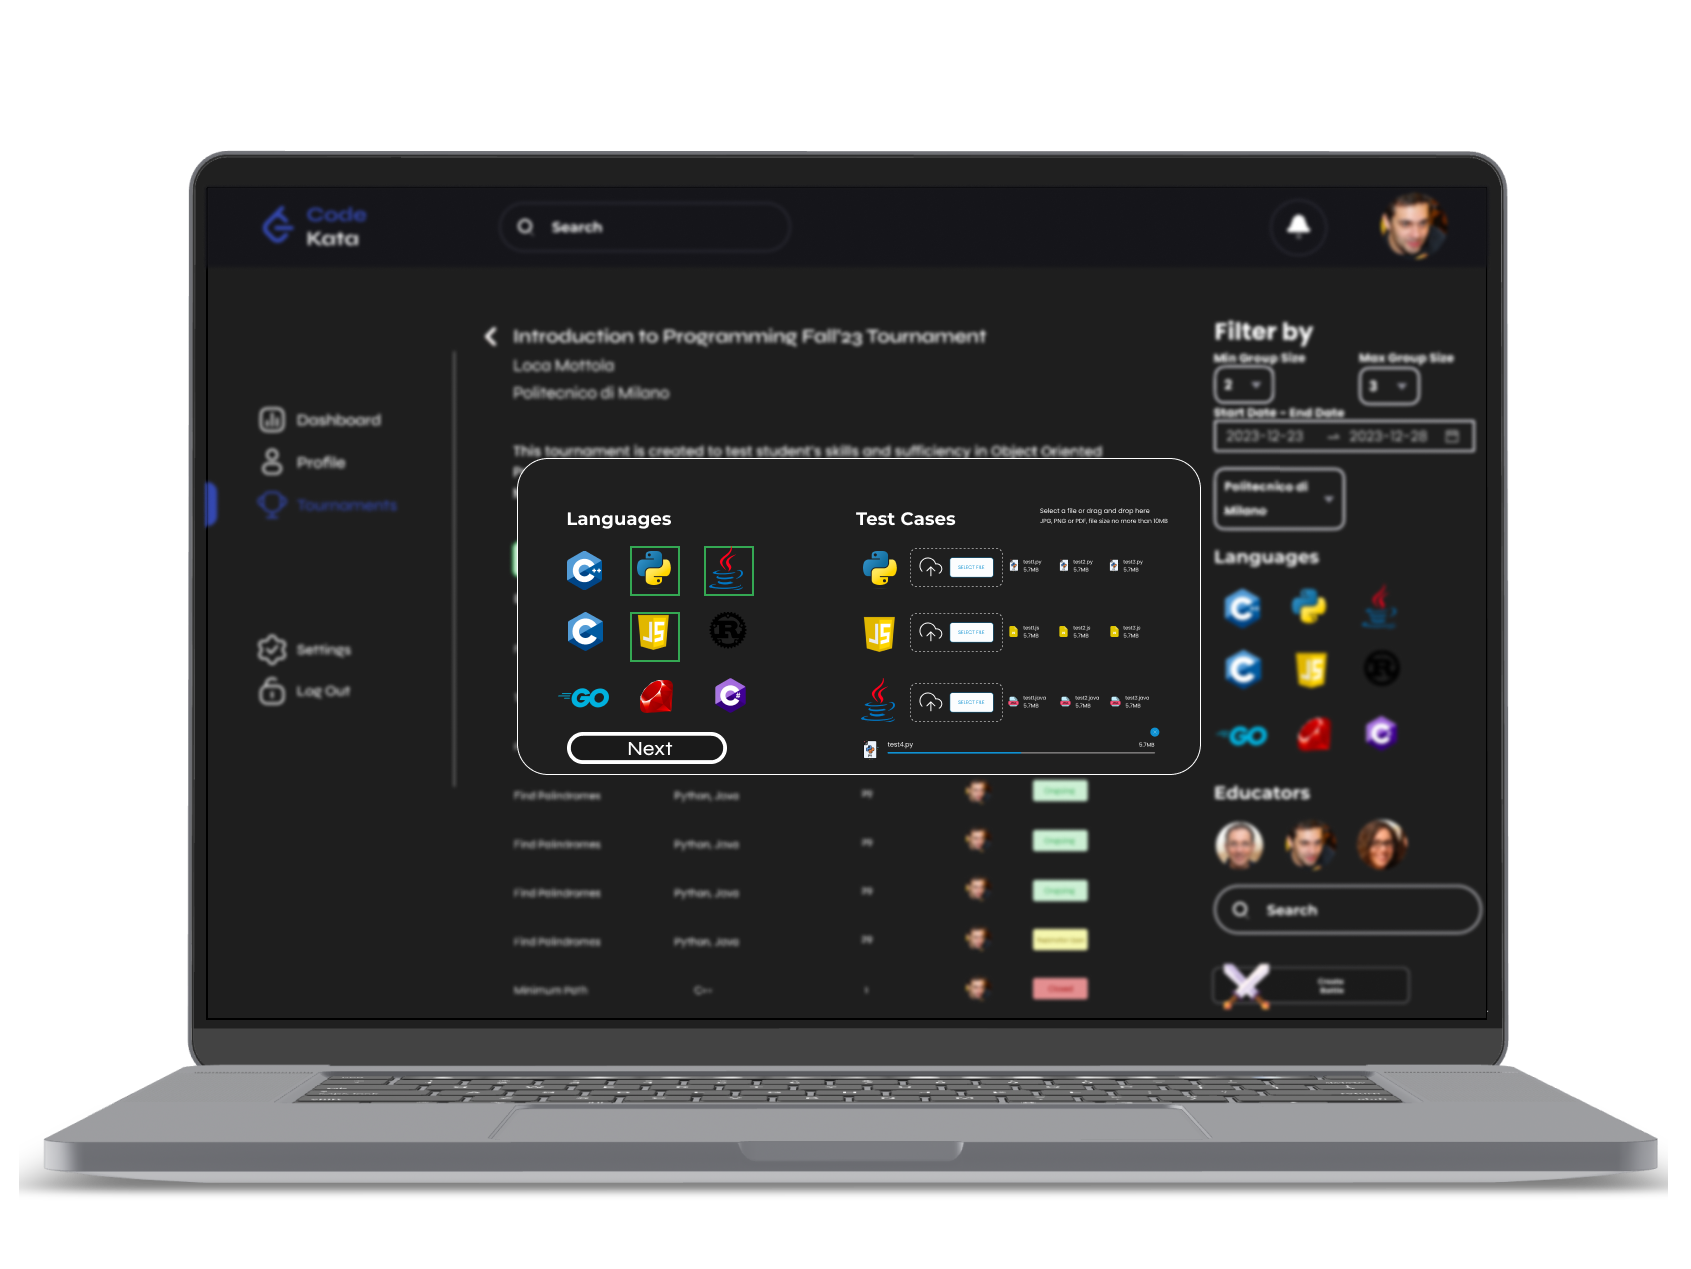
\includegraphics[scale=0.13]{Images/ui-ux/educator_creates_battle/educator_creates_battle_4.png}
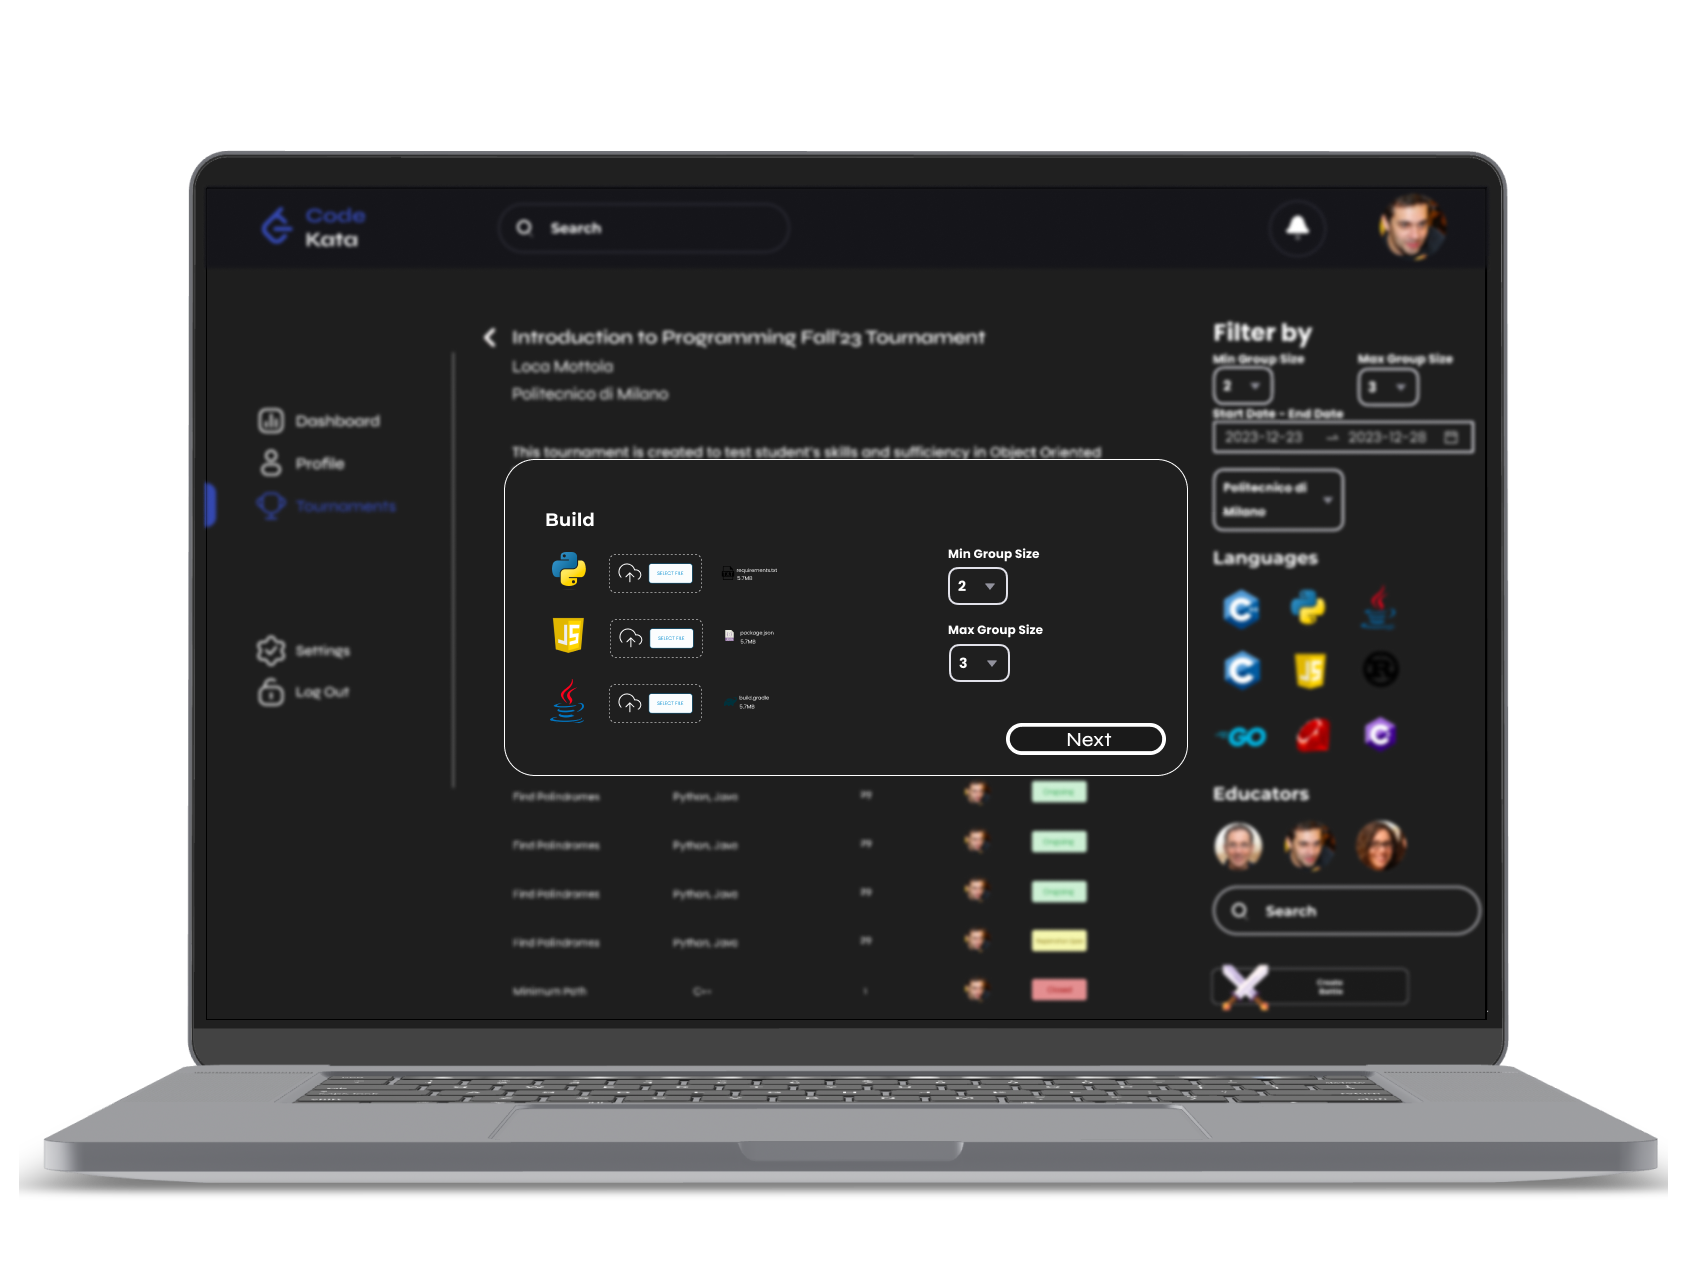
\includegraphics[scale=0.13]{Images/ui-ux/educator_creates_battle/educator_creates_battle_5.png}
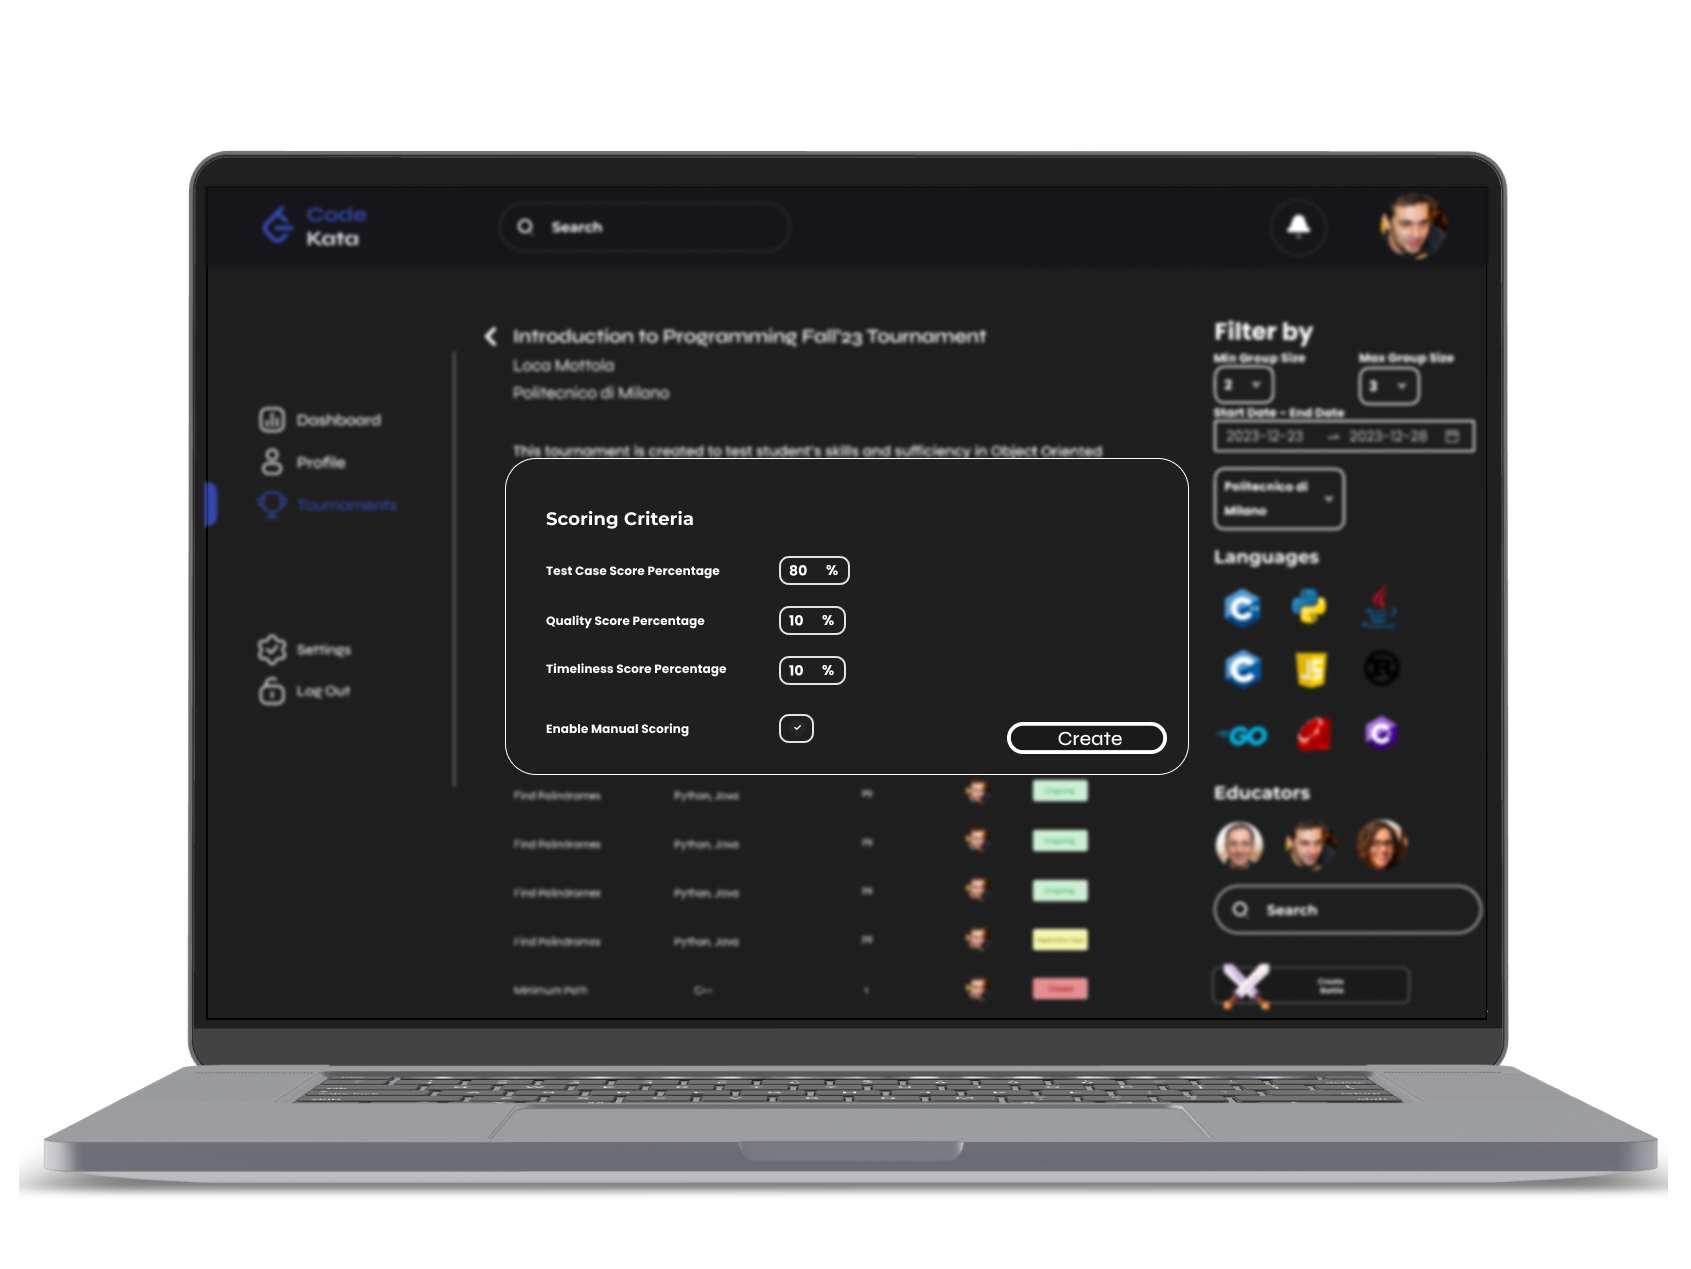
\includegraphics[scale=0.13]{Images/ui-ux/educator_creates_battle/educator_creates_battle_6.png}
        (l) Educator Creates Battle
\end{center}
\newpage
\begin{center}
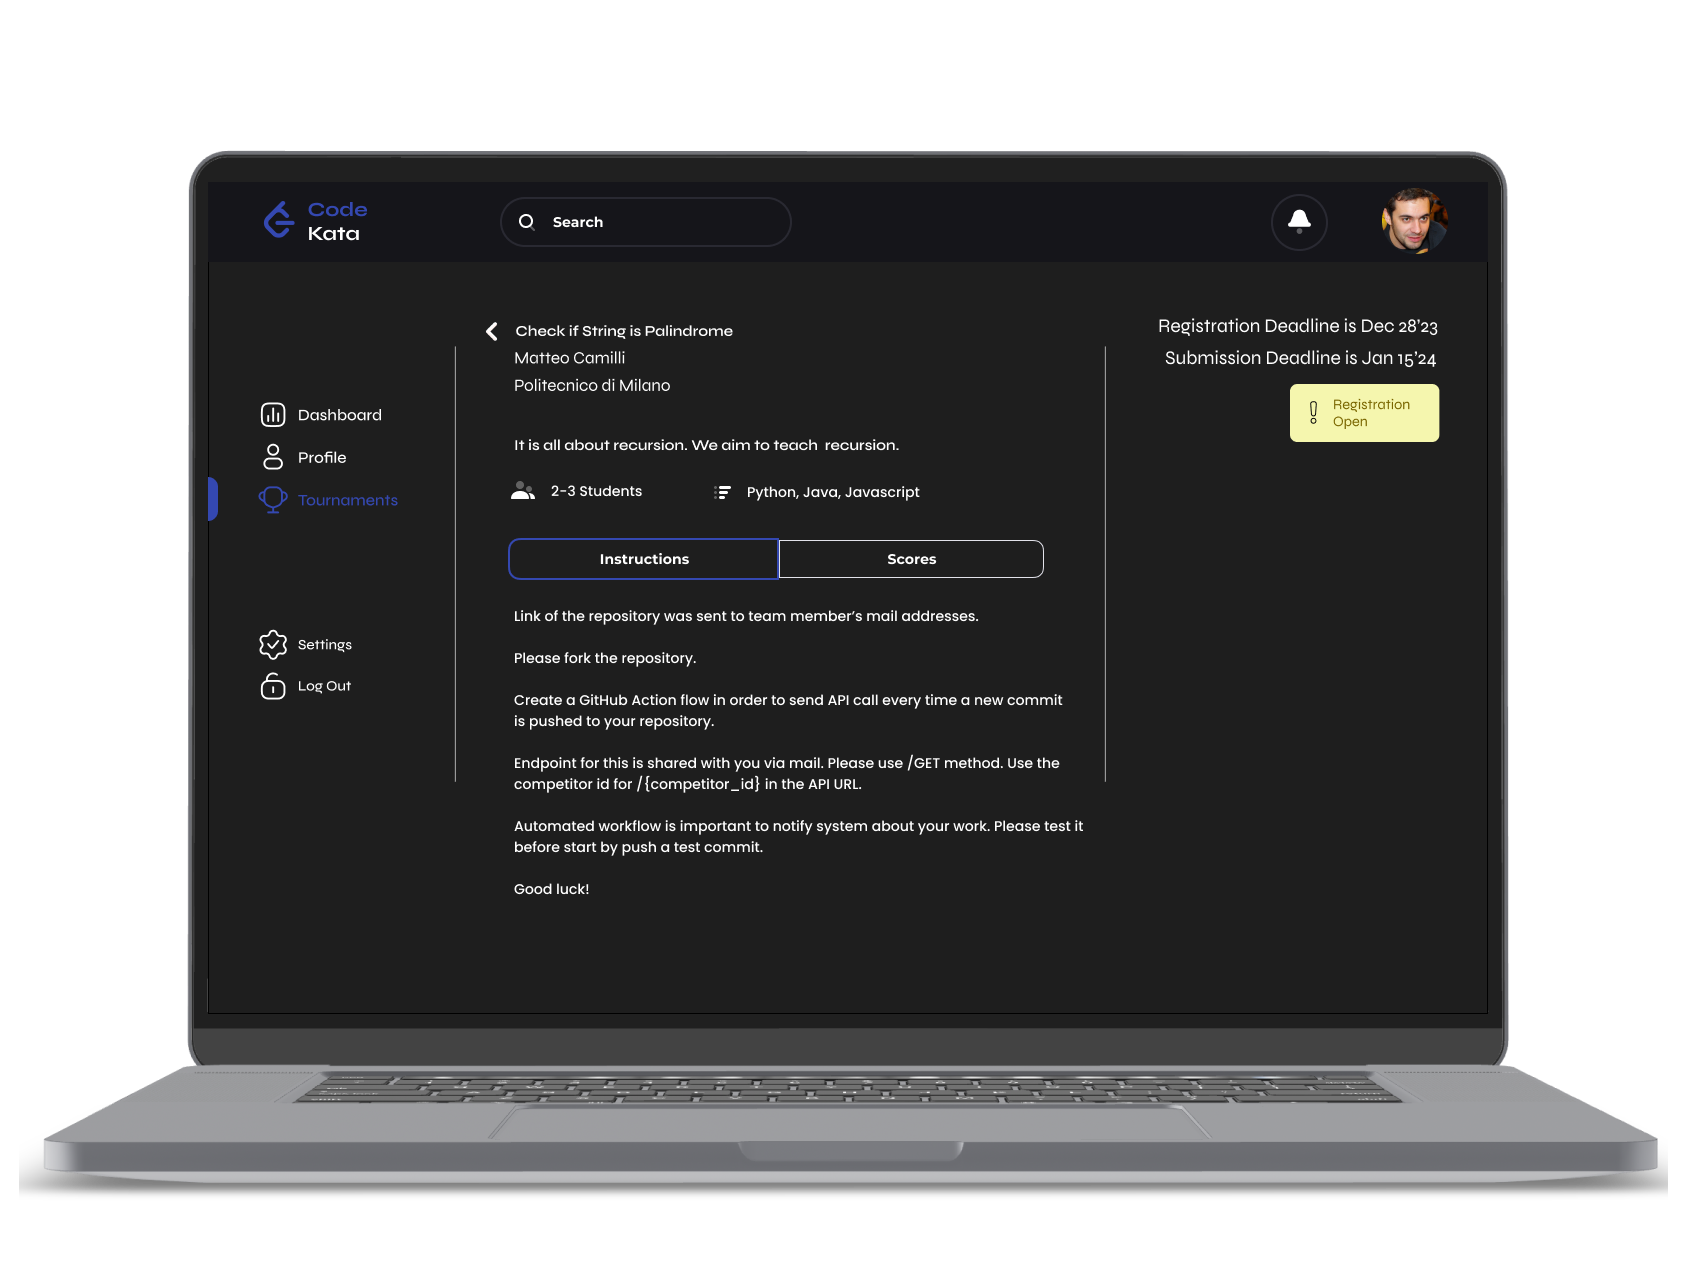
\includegraphics[scale=0.13]{Images/ui-ux/educator_battle/educator_battle_1.png}
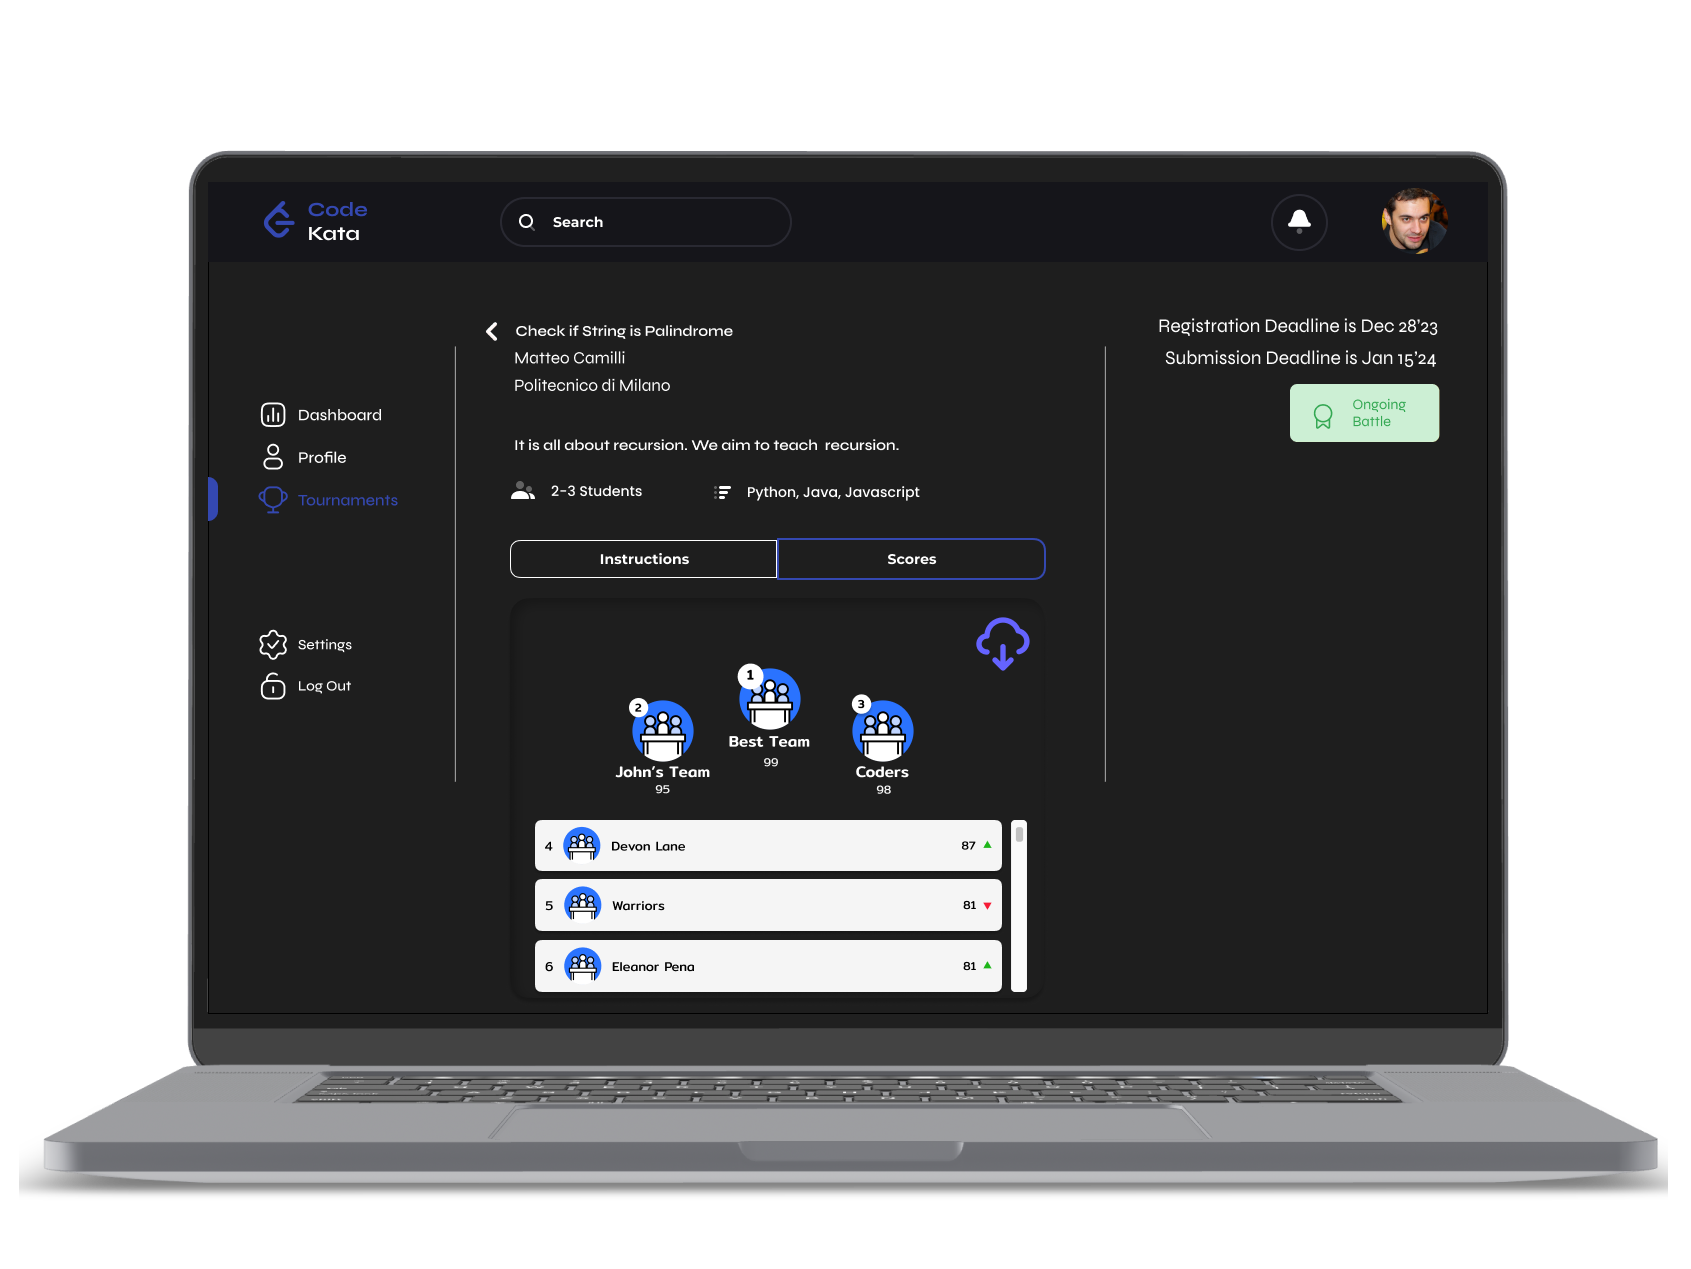
\includegraphics[scale=0.13]{Images/ui-ux/educator_battle/educator_battle_2.png}
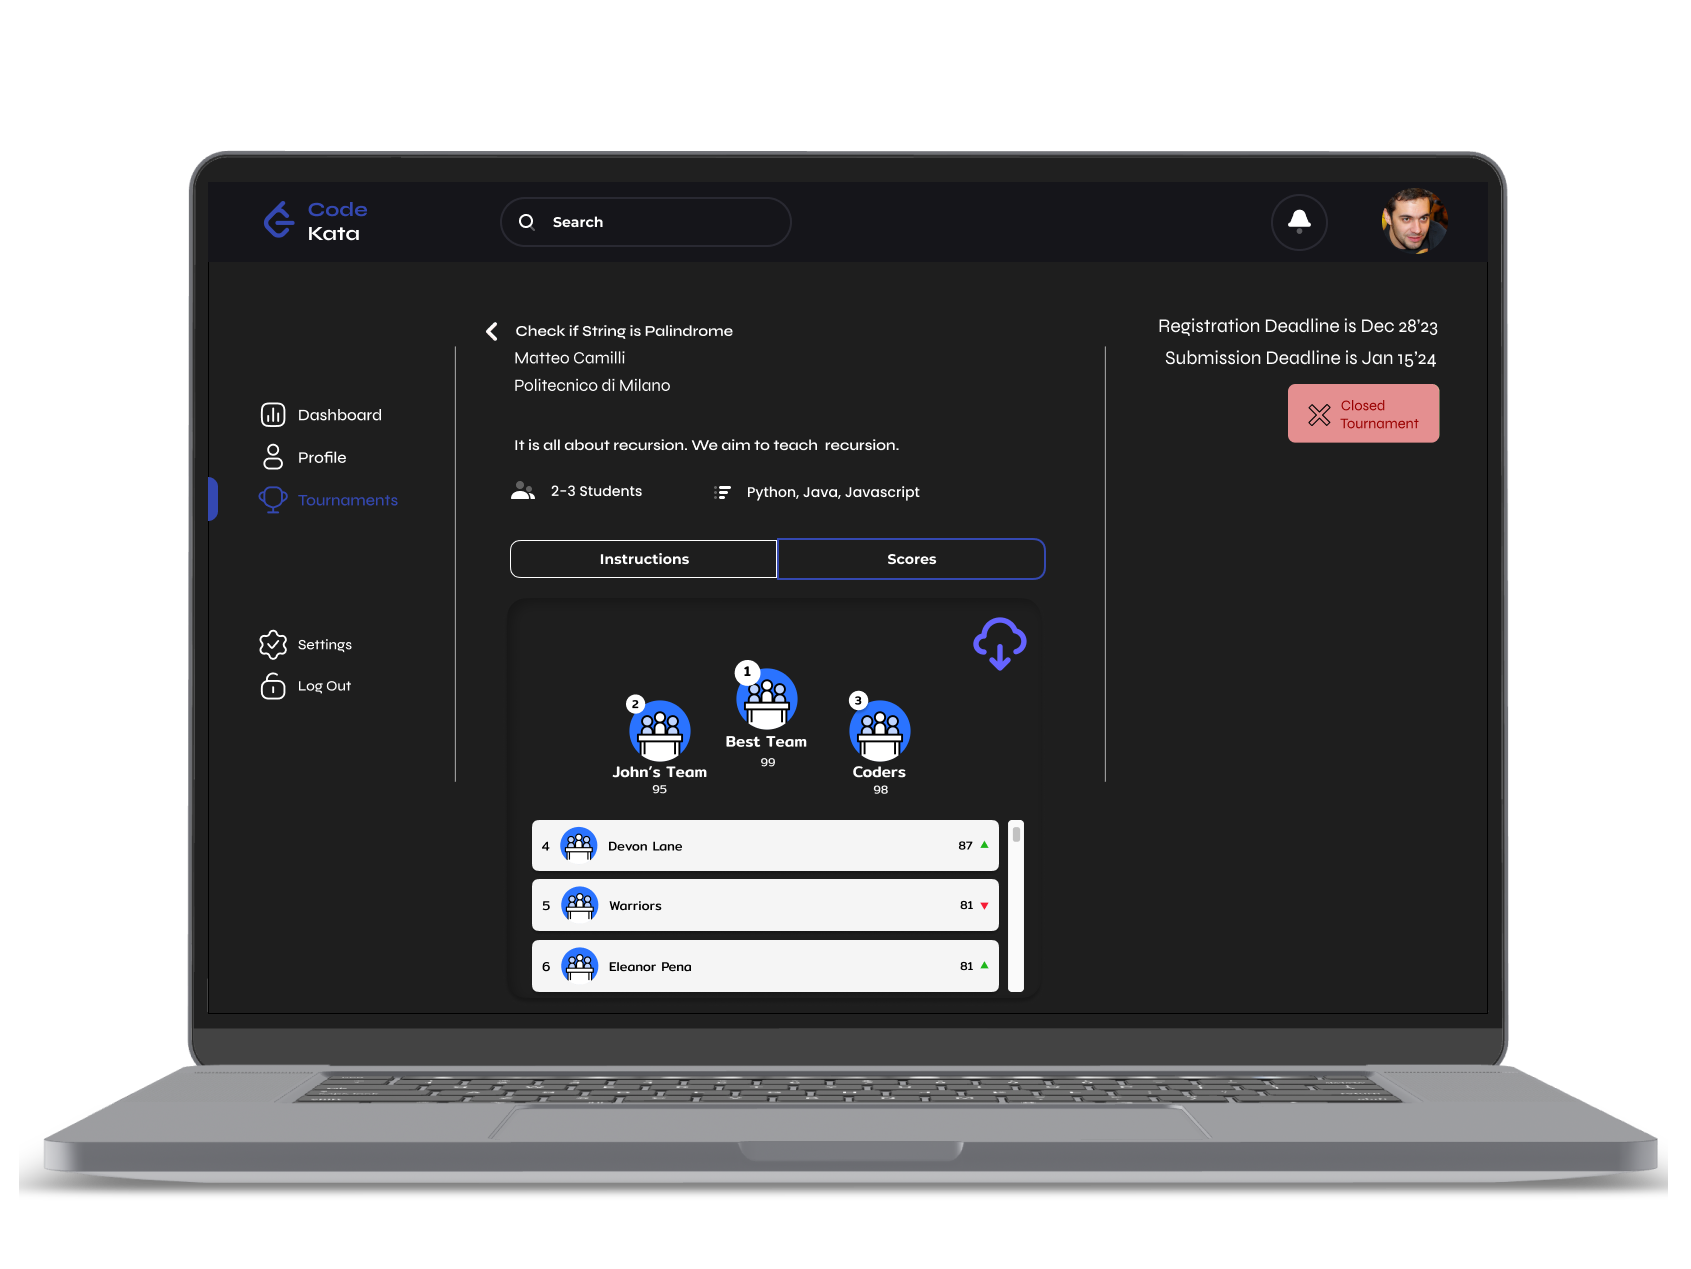
\includegraphics[scale=0.13]{Images/ui-ux/educator_battle/educator_battle_3.png}
\\ (m) Educator visits Battle
\end{center}
\newpage
\begin{center}
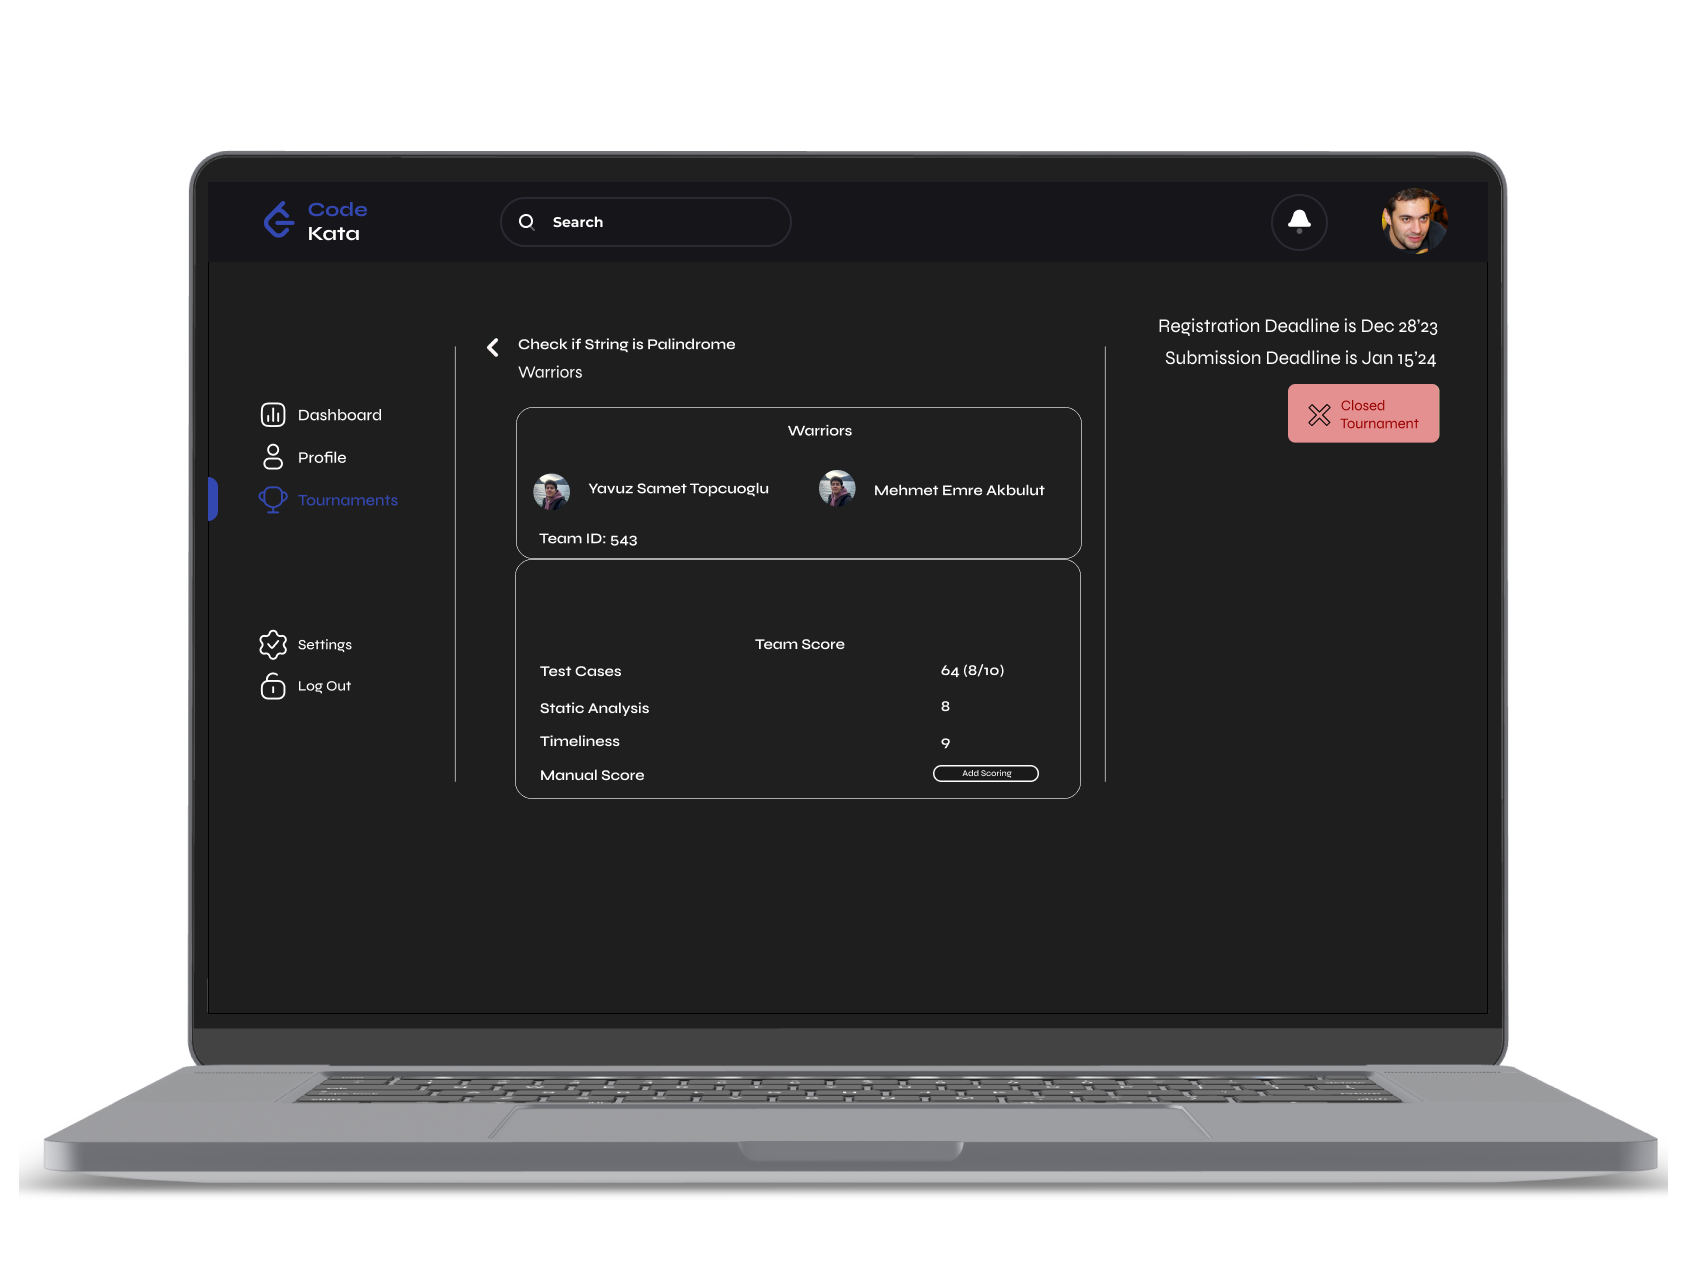
\includegraphics[scale=0.13]{Images/ui-ux/educator_team/educator_team_1.png}
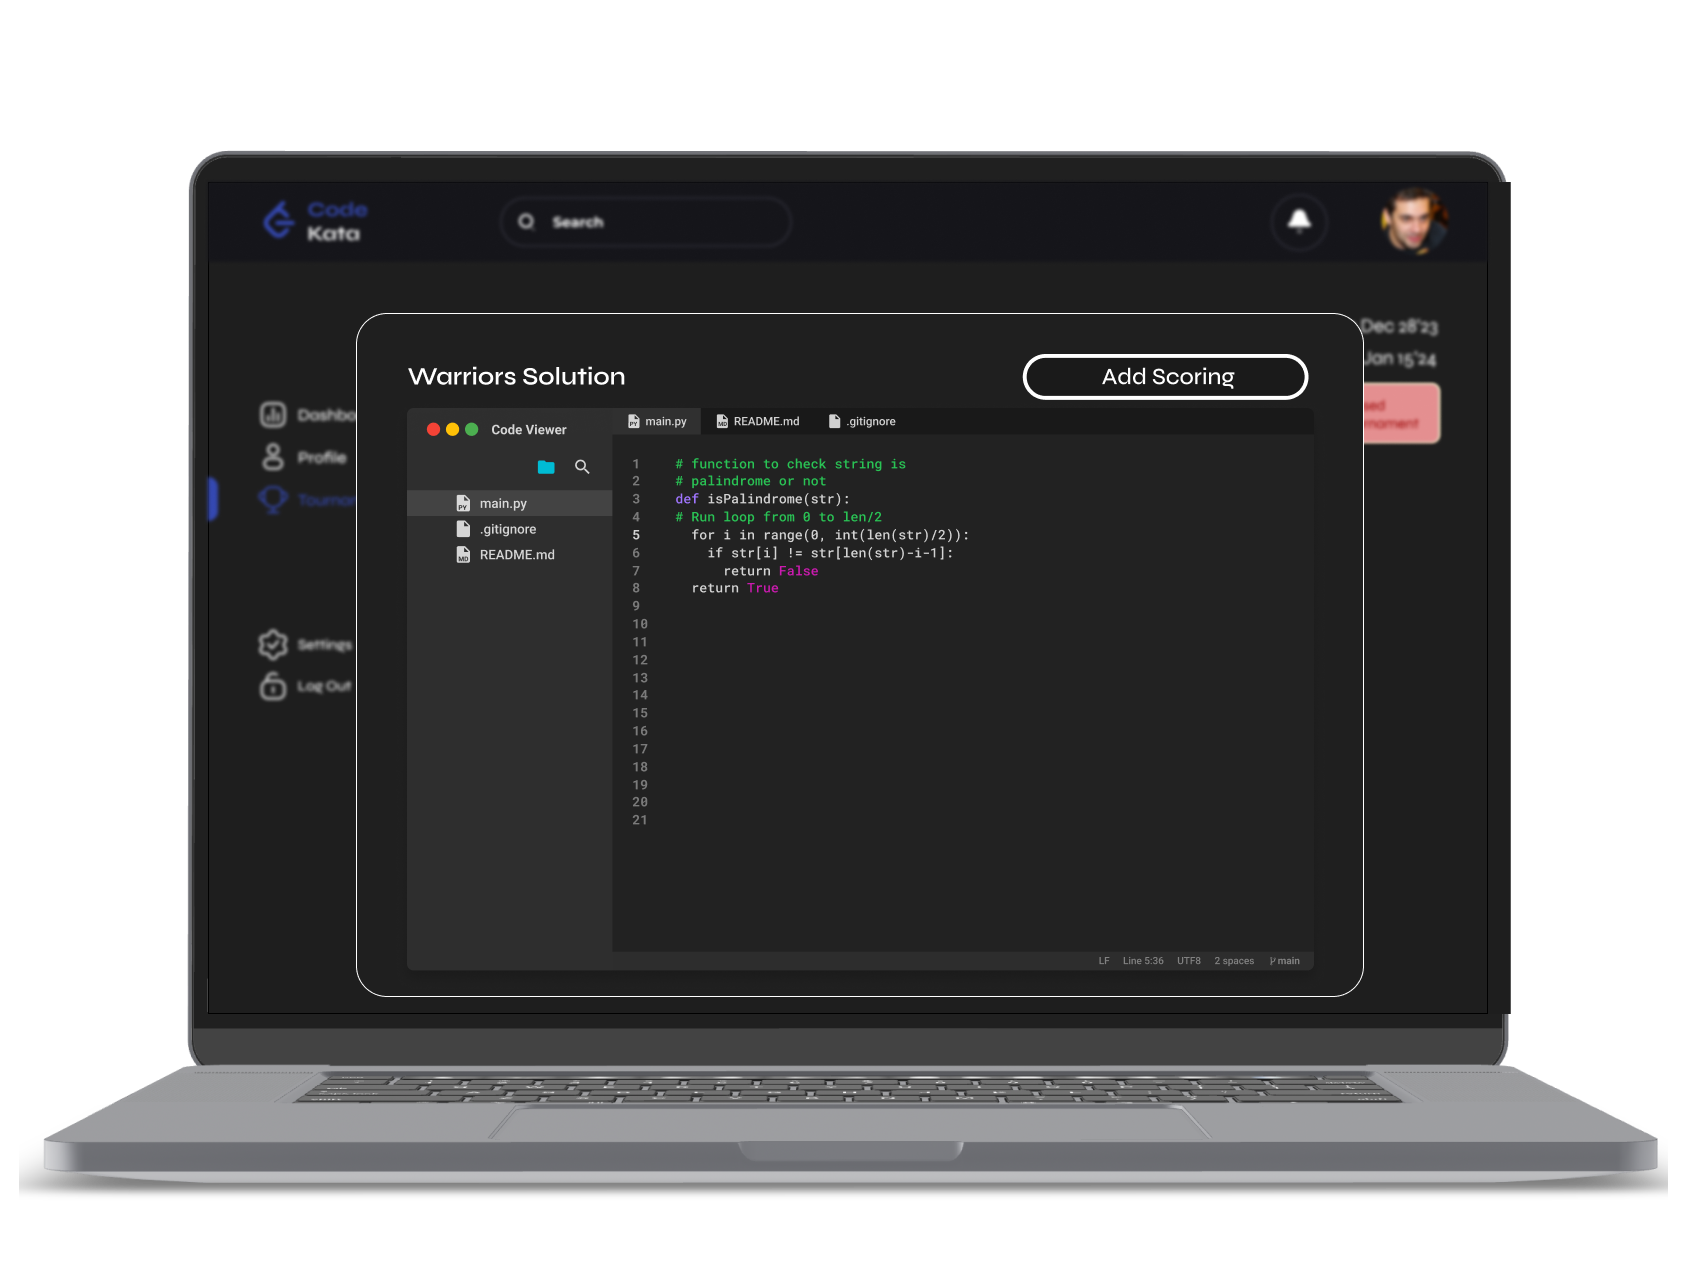
\includegraphics[scale=0.13]{Images/ui-ux/educator_team/educator_team_2.png}
\includegraphics[scale=0.13]{Images/ui-ux/educator_team/educator_team_3.png}
\includegraphics[scale=0.13]{Images/ui-ux/educator_team/educator_team_4.png}
        (n) Educator, Team and Manual Scoring
\end{center}
\begin{center}
\includegraphics[scale=0.13]{Images/ui-ux/educator_profile_settings/educator_profile.png}
\includegraphics[scale=0.13]{Images/ui-ux/educator_profile_settings/educator_settings.png}
        (o) Educator Profile and Settings
\end{center}
\newpage
\begin{center}
\includegraphics[scale=0.13]{Images/ui-ux/educator_end_tournament/educator_end_tournament.png}
\includegraphics[scale=0.13]{Images/ui-ux/educator_end_tournament/educator_end_tournament_1.png}
        (p) Educator Ends Tournament
\end{center}
\newpage
    
\subsubsection{Hardware Interfaces}
The CodeKataBattle platform operates entirely through web interfaces, eliminating the need for specialized hardware interfaces. Users can access the platform using standard web-enabled devices, such as computers, tablets, and smartphones. The platform is designed to function within a web browser, requiring no specific hardware beyond a device capable of running a modern browser and accessing the internet. This approach ensures broad accessibility without necessitating particular hardware configurations, making the platform versatile and user-friendly across various hardware setups. However, for optimal experience, at least 2GB of RAM and a minimum of 1GB of free space are recommended for browser caching and temporary files.

\subsubsection{Software Interfaces}
Our platform CKB interfaces with various software systems:

\begin{itemize}
    \item \textbf{Web Browsers:} Platform operates on web browsers. For universal access and easy use, it is compatible with major browsers like Chrome, Edge, Safari, Opera, and Firefox.

    \item \textbf{GitHub API:} Integrated for creating coding repositories and managing code \textit{submission} processes.

    \item \textbf{Sandboxing:} To create an isolated testing environment, this approach helps to create a reliable running environment while calculating test case scores.

    \item \textbf{Static Analysis Tool:} An external API will be integrated for scoring the quality aspect of the code with static analysis. 

    \item \textbf{Database Technology:} The data in the platform is consistent and needs to be stored in a database.

    \item \textbf{Hosting:} Our platform needs a web service that provides secure, resizable compute capacity in the cloud for web server and database hosting.

    \item \textbf{Cloud File Storage:} The files will be stored using object storage through a web service interface deployed in the cloud.
    \item \textbf{Email Service:} A simple Email Service will be used to send automated email notifications.
\end{itemize}

\subsubsection{Communication Interfaces}
Our platform utilises various communication systems:

\begin{itemize}
    \item \textbf{HTTPS:} For secure connection over the internet.

    \item \textbf{RESTful APIs:} We have RESTful APIs to communicate with the requests coming from GitHub Actions and the web application.

    \item \textbf{SMTP:} It is used to manage to send automated emails.
\end{itemize}


\subsection{Functional Requirements}
\subsubsection{Use Case Diagram}
\label{sec:Use Case Diagram}

\begin{figure}[H]
    \centering
    \includegraphics[scale=0.25]{Images/usecasefinal.drawio.png}
    \caption{Use Case Diagram}
\end{figure}


Unregistered User Actor has been used to illustrate the Registration Use Case. Similarly, the Registered User Actor has been used to show the Authentication Use Case. Other user actors are assumed to be registered and authenticated.

\\

Our system is composed of two main user types: Student and Educator. In the use case diagram, we showed common use cases with the Authenticated User actor. Authenticated User, simply every user registered to the platform, can view Tournaments, Battles, and their rankings with different filters and search options. Moreover, Registered User has the capability of viewing their profile and editing settings.

\\

Use case related Educator and Student Actors summarizes the goal of these users in the system.

\\

Invitee Student and Invitee Educator Actors are used to demonstrate use cases for tournament (for educators) and team (for students) invitations.

\\

GitHub System Boundary contains use cases about code submission with the participation of GitHub API Actor.

\subsubsection{Use Cases}

The Use Case Tables below, depict the possible use cases in detail. We tried to cover all the use cases that are included in the Use Case Diagram (see \hyperref[sec:Use Case Diagram]{3.2.1}). However, to reduce the complexity and the number of tables, some use cases that are strongly related to each other have been introduced in the same use case table. To keep track of them, they are written in \textit{italic} in the Event Flow if they occur. Additionally, the Related Use Case(s) row is added to the tables, to see explicitly which use cases from the Use Case Diagram are included in the table. 

\newpage
\begin{enumerate}
    \item Register
    \begin{center}
        \begin{tabular}{ | m{10em} | m{10cm}| } 
          \hline
          \textbf{Name} & Register  \\ 
          \hline
         \textbf{Actor(s)} & Unregistered User \\ 
          \hline
          \textbf{Entry Condition} & The user is unregistered to the platform. \\ 
          \hline
          \textbf{Event Flow} & 
          \begin{enumerate}[(1)]
              \item The actor enters the platform and clicks the Sign Up button.
              \item The actor fills out the registration form by providing email, password, name, surname, and institution information.
              \item The actor clicks the Sign Up button to \textit{register}.
          \end{enumerate} \\
          \hline
          \textbf{Exit Condition} & The actor is registered and the Login page is displayed.  \\ 
          \hline
          \textbf{Related Use Case(s)} & 
            \begin{itemize}
                \item \textit{Register}
            \end{itemize}  \\ 
          \hline
        \end{tabular}
        \captionof{table}{$UC_{1}$ - Register}\label{tbl:uc1}
    \end{center}

 
    
    \item Login
    \begin{center}
    \begin{tabular}{ | m{10em} | m{10cm}| } 
      \hline
      \textbf{Name} & Login (i.e. Authenticate)  \\ 
      \hline
      \textbf{Actor(s)} & Registered User \\ 
      \hline
      \textbf{Entry Condition} & The user is already registered to the platform. \\ 
      \hline
      \textbf{Event Flow} & 
          \begin{enumerate}[(1)]
              \item The actor enters the platform web page.
              \item The actor fills out the form by providing an email address and a password.
              \item The actor clicks the Login button to \textit{authenticate}.
          \end{enumerate}
      \\ 
      \hline
      \textbf{Exit Condition} & The actor is logged in and the dashboard is displayed.  \\ 
      \hline
      \textbf{Exception(s)} & 
      \begin{itemize}
          \item The email and password do not match.
      \end{itemize}
      \\ 
      \hline
      \textbf{Related Use Case(s)} & 
      \begin{itemize}
          \item \textit{Authenticate}
      \end{itemize}
      \\
      \hline
    \end{tabular}
            \captionof{table}{$UC_{2}$ - Login}\label{tbl:uc2}
\end{center}
\newpage
\item View a Tournament
    \begin{center}
    \begin{tabular}{ | m{10em} | m{10cm}| } 
      \hline
      \textbf{Name} & View a Tournament  \\ 
      \hline
      \textbf{Actor(s)} & Authenticated User \\ 
      \hline
      \textbf{Entry Condition} & The actor is logged in. \\ 
      \hline
      \textbf{Event Flow} & 
          \begin{enumerate}[(1)]
              \item The actor clicks the Tournaments button from the sidebar.
              \item In the tournaments page, the actor \textit{views all tournaments} as cards.
              \item The actor \textit{filters tournaments} by registered filter.
              \item The actor \textit{sorts tournaments} by \# of participants.
              \item The actor clicks the first tournament card to \textit{view a specific tournament}.
          \end{enumerate}
      \\ 
      \hline
      \textbf{Exit Condition} & The specific tournament that the actor wants to view is displayed.  \\ 
      \hline
      \textbf{Exception(s)} & 
      \begin{itemize}
          \item There are no existing tournaments.
          \item There are no tournaments with the filter set by the actor.
      \end{itemize}
          \\ 
      \hline
      \textbf{Related Use Case(s)} & 
      \begin{itemize}
          \item \textit{View All Tournaments}
          \item \textit{Filter Tournaments}
          \begin{itemize}
              \item \textit{Filter by Registration Status}
          \end{itemize}
          \item \textit{Sort Tournaments}
          \begin{itemize}
            \item \textit{Sort by \# of Participants}
          \end{itemize}
          \item \textit{View a Specific Tournament}
      \end{itemize}
          \\ 
      \hline
    \end{tabular}
            \captionof{table}{$UC_{3}$ - View Tournament}\label{tbl:uc3}
\end{center}

\newpage

\item View the Tournament Leaderboard
\begin{center}
    \begin{tabular}{ | m{10em} | m{10cm}| } 
      \hline
      \textbf{Name} & View the Tournament Leaderboard \\ 
      \hline
      \textbf{Actor(s)} & Authenticated User \\ 
      \hline
      \textbf{Entry Condition} & The actor is viewing a specific tournament. \\ 
      \hline
      \textbf{Event Flow} & 
          \begin{enumerate}[(1)]
              \item The actor clicks the Leaderboard button to \textit{view the tournament leaderboard}.
          \end{enumerate}
      \\ 
      \hline
      \textbf{Exit Condition} & The leaderboard of that tournament is displayed.  \\ 
      \hline
      \textbf{Related Use Case(s)} & 
      \begin{itemize}
      \item \textit{View the Tournament Leaderboard}
      \end{itemize}
          \\ 
      \hline
    \end{tabular}
    \captionof{table}{$UC_{4}$ - View Tournament Leaderboard}\label{tbl:uc4}
\end{center}


\item View a Battle
    \begin{center}
    \begin{tabular}{ | m{10em} | m{10cm}| } 
      \hline
      \textbf{Name} & View a Battle  \\ 
      \hline
      \textbf{Actor(s)} & Authenticated User \\ 
      \hline
      \textbf{Entry Condition} & The actor is viewing a specific tournament. \\ 
      \hline
      \textbf{Event Flow} & 
          \begin{enumerate}[(1)]
              \item The actor \textit{views the battles of the tournament} in that tournament's page.
              \item The actor \textit{searches battles} using the search bar at the bottom of the page.
              \item The actor \textit{filters battles} using the filter section on the right-hand side of the page.
              \item The actor chooses one of the results to \textit{view a specific battle}.
          \end{enumerate}
      \\ 
      \hline
      \textbf{Exit Condition} & The specific battle that the actor wants to view is displayed.  \\ 
      \hline
      \textbf{Exception(s)} & 
      \begin{itemize}
          \item There are no existing battles in that tournament.
          \item There are no battles with the filters set by the actor.
      \end{itemize}
          \\ 
      \hline
      \textbf{Related Use Case(s)} & 
      \begin{itemize}
          \item \textit{View Battles of the Tournament}
          \item \textit{Search Battles}
          \item \textit{Filter Battles}
          \item \textit{View a Specific Battle}
      \end{itemize}
          \\ 
      \hline
    \end{tabular}
    \captionof{table}{$UC_{5}$ - View Battle}\label{tbl:uc5}
\end{center}


\newpage


\item View the Battle Instructions
\begin{center}
    \begin{tabular}{ | m{10em} | m{10cm}| } 
      \hline
      \textbf{Name} & View the Battle Instructions \\ 
      \hline
      \textbf{Actor(s)} & Authenticated User \\ 
      \hline
      \textbf{Entry Condition} & The actor is viewing a specific battle. \\ 
      \hline
      \textbf{Event Flow} & 
          \begin{enumerate}[(1)]
              \item The actor clicks the Instructions button to \textit{view the battle instructions}.
          \end{enumerate}
      \\ 
      \hline
      \textbf{Exit Condition} & The instructions of that battle are displayed.  \\ 
      \hline
      \textbf{Related Use Case(s)} & 
      \begin{itemize}
          \item \textit{View the Battle Instructions}
      \end{itemize}
          \\ 
      \hline
    \end{tabular}
    \captionof{table}{$UC_{6}$ - View Battle Instructions}\label{tbl:uc6}
\end{center}

\item View the Battle Rankings
\begin{center}
    \begin{tabular}{ | m{10em} | m{10cm}| } 
      \hline
      \textbf{Name} & View the Battle Rankings \\ 
      \hline
      \textbf{Actor(s)} & Authenticated User \\ 
      \hline
      \textbf{Entry Condition} & The actor is viewing a specific battle. \\ 
      \hline
      \textbf{Event Flow} & 
          \begin{enumerate}[(1)]
              \item The actor clicks the Scores button to \textit{view the battle rankings}.
          \end{enumerate}
      \\ 
      \hline
      \textbf{Exit Condition} & The rankings of that battle are displayed.  \\ 
      \hline
      \textbf{Related Use Case(s)} & 
      \begin{itemize}
\item \textit{View the Battle Rankings}
      \end{itemize}
          \\ 
      \hline
    \end{tabular}
    \captionof{table}{$UC_{7}$ - View Battle Rankings}\label{tbl:uc7}
\end{center}

\newpage
\item Inspect a Submission
\begin{center}
    \begin{tabular}{ | m{10em} | m{10cm}| } 
      \hline
      \textbf{Name} & Inspect a Submission \\ 
      \hline
      \textbf{Actor(s)} & Educator \\ 
      \hline
      \textbf{Entry Condition} & The actor is viewing the battle rankings of a specific battle. \\ 
      \hline
      \textbf{Event Flow} & 
          \begin{enumerate}[(1)]
              \item The actor clicks one of the teams from the rankings table to \textit{view the team's submission}.
              \item The actor looks at the code and decides to \textit{manually evaluate}.
              \item The actor enters the bonus points in the respective field and clicks the Add Scoring button.
          \end{enumerate}
      \\ 
      \hline
      \textbf{Exit Condition} & The total score after manual evaluation of that team are displayed.  \\ 
      \hline
      \textbf{Exception(s)} & 
      \begin{itemize}
          \item The manual scoring is not enabled.
      \end{itemize}
          \\ 
      \hline
      \textbf{Related Use Case(s)} & 
      \begin{itemize}
\item \textit{View the Code of a Team}
\item \textit{Manual Evaluation}
      \end{itemize}
          \\ 
      \hline
    \end{tabular}
    \captionof{table}{$UC_{8}$ - Inspect Submission}\label{tbl:uc8}
\end{center}


\newpage


\item Search Tournaments
\begin{center}
    \begin{tabular}{ | m{10em} | m{10cm}| } 
      \hline
      \textbf{Name} & Search Tournament  \\ 
      \hline
      \textbf{Actor(s)} & Authenticated User \\ 
      \hline
      \textbf{Entry Condition} & The user is logged in. \\ 
      \hline
      \textbf{Event Flow} & 
          \begin{enumerate}[(1)]
              \item The actor clicks the button in the search area to select the search criteria.
              \item The actor sees three buttons: \textit{Search by Educators}, \textit{Search by Titles}, \textit{Search by Institutions} and chooses to search by title.
              \item The actor writes "Fall'23 Tournament" to the search bar and hits enter to \textit{search tournament}.
          \end{enumerate}
      \\ 
      \hline
      \textbf{Exit Condition} & The tournaments with the corresponding title are displayed.  \\ 
      \hline
      \textbf{Exception(s)} & 
      \begin{itemize}
          \item The tournament with the given title does not exist.
      \end{itemize}
          \\ 
      \hline
      \textbf{Related Use Case(s)} & 
      \begin{itemize}
          \item \textit{Search by Educator}
          \item \textit{Search by Title}
          \item \textit{Search by Institution}
          \item \textit{Search Tournament}
      \end{itemize}
          \\ 
      \hline
    \end{tabular}
        \captionof{table}{$UC_{9}$ - Search Tournaments}\label{tbl:uc9}
\end{center}


\item Register to a Tournament
\begin{center}
    \begin{tabular}{ | m{10em} | m{10cm}| } 
      \hline
      \textbf{Name} & Register to a Tournament  \\ 
      \hline
      \textbf{Actor(s)} & Student \\ 
      \hline
      \textbf{Entry Condition} & The actor is logged in and the tournaments page is on display.\\ 
      \hline
      \textbf{Event Flow} & 
          \begin{enumerate}[(1)]
              \item The actor clicks a card of a tournament in which s/he is not registered.
              \item The actor clicks the Register button in the pop-up to \textit{register the tournament}.
          \end{enumerate}
      \\ 
      \hline
      \textbf{Exit Condition} & The actor is registered to the tournament and the page of that tournament is displayed.  \\ 
      \hline
      \textbf{Exception(s)} & 
      \begin{itemize}
          \item There are not any tournaments with not registered status.
      \end{itemize}
          \\ 
      \hline
      \textbf{Related Use Case(s)} & 
      \begin{itemize}
          \item \textit{Register Tournament}
      \end{itemize}
          \\ 
      \hline
    \end{tabular}
    \captionof{table}{$UC_{10}$ - Register to a Tournament}\label{tbl:uc10}
\end{center}


\newpage


\item Register to a Battle
\begin{center}
    \begin{tabular}{ | m{10em} | m{10cm}| } 
      \hline
      \textbf{Name} & Register to a Battle  \\ 
      \hline
      \textbf{Actor(s)} & Student \\ 
      \hline
      \textbf{Entry Condition} & The actor registered to the tournament in which the battle takes place and that tournament's page is on display. \\ 
      \hline
      \textbf{Event Flow} & 
          \begin{enumerate}[(1)]
              \item The actor clicks a register button next to the battle that s/he wants to participate in.
              \item The actor clicks the Register button in the pop-up.
              \item The actor chooses between to \textit{form a team} and to \textit{register individually}. 
              \item If there is going to be a team, the actor \textit{sets a team name} and \textit{invites colleagues}.
              \item The actor clicks the Complete button to \textit{register to the battle}.
          \end{enumerate}
      \\ 
      \hline
      \textbf{Exit Condition} & 
      \begin{itemize}
          \item If registered individually, the actor is registered to the battle.
          \item If a team is formed, the invitation requests are sent to the colleagues.
      \end{itemize}
        \\ 
      \hline
      \textbf{Exception(s)} & 
      \begin{itemize}
          \item The actor is already registered for all battles in that tournament.
      \end{itemize}
          \\ 
      \hline
      \textbf{Related Use Case(s)} & 
      \begin{itemize}
          \item \textit{Register Battle}
          \item \textit{Form Team}
          \item \textit{Register Individually}
          \item \textit{Invite Colleagues}
          \item \textit{Set Team Name}
      \end{itemize}
          \\ 
      \hline
    \end{tabular}
        \captionof{table}{$UC_{11}$ - Register to a Battle}\label{tbl:uc11}
\end{center}


\newpage

\item Complete the Team Registration for the Battle
\begin{center}
    \begin{tabular}{ | m{10em} | m{10cm}| } 
      \hline
      \textbf{Name} & Complete the Team Registration for the Battle  \\ 
      \hline
      \textbf{Actor(s)} & Student \\ 
      \hline
      \textbf{Entry Condition} & The specific battle that the actor wants to complete the registration is on display. \\ 
      \hline
      \textbf{Event Flow} & 
          \begin{enumerate}[(1)]
              \item The actor can see which colleague accepted the invitation and which colleague rejected it.
              \item The actor can finalize the team formation if there are enough colleagues on the team by using the Finalize button, or discard the team and battle registration entirely by using the Decline button to \textit{complete the team registration}.
          \end{enumerate}
      \\ 
      \hline
      \textbf{Exit Condition} & 
      \begin{itemize}
          \item If finalized, the team is registered to the battle.
          \item If declined, the team is not registered to the battle and the dashboard is displayed.
      \end{itemize}\\ 
      \hline
      \textbf{Related Use Case(s)} & 
      \begin{itemize}
          \item \textit{Complete the Team Registration}
      \end{itemize}
          \\ 
      \hline
    \end{tabular}
        \captionof{table}{$UC_{12}$ - Complete the Team Registration}\label{tbl:uc12}
\end{center}


\item Respond to the Team Invitation
\begin{center}
    \begin{tabular}{ | m{10em} | m{10cm}| } 
      \hline
      \textbf{Name} & Respond to the Team Invitation  \\ 
      \hline
      \textbf{Actor(s)} & Invitee Student \\ 
      \hline
      \textbf{Entry Condition} & The actor is logged in and invited to a team by another student.  \\ 
      \hline
      \textbf{Event Flow} & 
          \begin{enumerate}[(1)]
              \item The actor opens up the notifications and sees the invitation to join a team formed by another student.
              \item The actor clicks the notification and a pop-up shows up.
              \item The actor can choose to \textit{Accept Invitation} by clicking the Accept button or \textit{Reject Invitation} by clicking the Reject button to \textit{respond to the invitation}.
          \end{enumerate}
      \\ 
      \hline
      \textbf{Exit Condition} & 
      \begin{itemize}
          \item If accepted, the specific battle is displayed.
          \item If rejected, the dashboard is displayed.
      \end{itemize}\\ 
      \hline
      \textbf{Related Use Case(s)} & 
      \begin{itemize}
          \item \textit{Accept Invitation}
          \item \textit{Reject Invitation}
          \item \textit{Respond to Team Invitation}
      \end{itemize}
          \\ 
      \hline
    \end{tabular}
        \captionof{table}{$UC_{13}$ - Respond to the Team Invitation}\label{tbl:uc13}
\end{center}



\newpage

\item Submission
\begin{center}
    \begin{tabular}{ | m{10em} | m{10cm}| } 
      \hline
      \textbf{Name} & Submission  \\ 
      \hline
      \textbf{Actor(s)} & Student, GitHub API, Static Analyser Tool \\ 
      \hline
      \textbf{Entry Condition} & The student actor forked the battle repository, and initiated GitHub Actions on their repository. \\ 
      \hline
      \textbf{Event Flow} & 
          \begin{enumerate}[(1)]
              \item The student actor \textit{sets up the necessary environment}.
              \item The student actor works on the problem and writes code. 
              \item The student actor \textit{commits code} to their repository to \textit{make the submission}.
              \item The GitHub API actor informs the CKB platform to pull the code.
              \item The CKB platform pulls the code from the team's repository.
              \item The platform \textit{calculates the score} of the submission with respect to test cases, timeliness, and quality aspects. 
              \item During the calculation of quality aspects, it uses the API provided by the Static Analyser Tool actor.
          \end{enumerate}
      \\ 
      \hline
      \textbf{Exit Condition} & The CKB platform assigns the score to the team. \\ 
      \hline
      \textbf{Exception(s)} & 
      \begin{itemize}
          \item The GitHub API stops responding.
          \item The Static Analyser Tool stops responding.
          \item The student is not able to provide a solution.
      \end{itemize}
          \\ 
      \hline
      \textbf{Related Use Case(s)} & 
      \begin{itemize}
          \item \textit{Submission}
          \item \textit{Set Up Environment}
          \item \textit{Code Commit}
          \item \textit{Score Calculation}
      \end{itemize}
          \\ 
      \hline
    \end{tabular}
    \captionof{table}{$UC_{14}$ - Submission}\label{tbl:uc14}
\end{center}

\newpage
\item View Profile
\begin{center}
    \begin{tabular}{ | m{10em} | m{10cm}| } 
      \hline
      \textbf{Name} & View Profile  \\ 
      \hline
      \textbf{Actor(s)} & Authenticated User \\ 
      \hline
      \textbf{Entry Condition} & The actor is logged in. \\ 
      \hline
      \textbf{Event Flow} & 
          \begin{enumerate}[(1)]
              \item The actor clicks the Profile button from the sidebar to \textit{view the profile}.
          \end{enumerate}
      \\ 
      \hline
      \textbf{Exit Condition} & The profile page is displayed.  \\ 
      \hline
      \textbf{Related Use Case(s)} & 
      \begin{itemize}
          \item \textit{View Profile}
      \end{itemize}
          \\ 
      \hline
    \end{tabular}
     \captionof{table}{$UC_{15}$ - View Profile}\label{tbl:uc15}
\end{center}


\newpage

\item See Own Tournaments
\begin{center}
    \begin{tabular}{ | m{10em} | m{10cm}| } 
      \hline
      \textbf{Name} & See Own Tournaments  \\ 
      \hline
      \textbf{Actor(s)} & Authenticated User \\ 
      \hline
      \textbf{Entry Condition} & The actor is on the profile page. \\ 
      \hline
      \textbf{Event Flow} & 
          \begin{enumerate}[(1)]
              \item The actor clicks the Tournaments icon to \textit{to see own tournaments}.
          \end{enumerate}
      \\ 
      \hline
      \textbf{Exit Condition} & The tournaments that the actor engaged (either closed, ongoing, or upcoming) are displayed.  \\ 
      \hline
      \textbf{Related Use Case(s)} & 
      \begin{itemize}
          \item \textit{See Own Tournaments}
      \end{itemize}
          \\ 
      \hline
      \textbf{Note(s)} & 
      \begin{itemize}
          \item Engage means registered for students, and created for educators.
      \end{itemize}
          \\ 
      \hline
    \end{tabular}
     \captionof{table}{$UC_{16}$ - See Own Tournaments}\label{tbl:uc16}
\end{center}

\item See Own Battles
\begin{center}
    \begin{tabular}{ | m{10em} | m{10cm}| } 
      \hline
      \textbf{Name} & See Own Battles  \\ 
      \hline
      \textbf{Actor(s)} & Authenticated User \\ 
      \hline
      \textbf{Entry Condition} & The actor is on the profile page. \\ 
      \hline
      \textbf{Event Flow} & 
          \begin{enumerate}[(1)]
              \item The actor clicks the Battles icon to \textit{to see own battles}.
          \end{enumerate}
      \\ 
      \hline
      \textbf{Exit Condition} &  The battles that the actor engaged (either closed, ongoing, or upcoming) are displayed.  \\ 
      \hline
      \textbf{Related Use Case(s)} & 
      \begin{itemize}
          \item \textit{See Own Battles}
      \end{itemize}
          \\ 
      \hline
      \textbf{Note(s)} & 
      \begin{itemize}
          \item Engage means registered for students, and created for educators.
      \end{itemize}
          \\ 
      \hline
    \end{tabular}
     \captionof{table}{$UC_{17}$ - See Own Battles}\label{tbl:uc17}
\end{center}

\newpage

\item Delete Profile
\begin{center}
    \begin{tabular}{ | m{10em} | m{10cm}| } 
      \hline
      \textbf{Name} & Delete Profile  \\ 
      \hline
      \textbf{Actor(s)} & Authenticated User \\ 
      \hline
      \textbf{Entry Condition} & The actor is on the profile page. \\ 
      \hline
      \textbf{Event Flow} & 
          \begin{enumerate}[(1)]
              \item The actor clicks the Delete Profile button.
          \end{enumerate}
      \\ 
      \hline
      \textbf{Exit Condition} & The actor is removed from the platform.  \\ 
      \hline
      \textbf{Exception(s)} & 
      \begin{itemize}
          \item The actor is of type Educator and s/he has an ongoing tournament that s/he created.
      \end{itemize}
          \\ 
      \hline
      \textbf{Related Use Case(s)} & 
      \begin{itemize}
          \item \textit{Delete Profile}
      \end{itemize}
          \\ 
      \hline
      \textbf{Note(s)} & 
      \begin{itemize}
          \item The educators who have an ongoing tournament created by themselves cannot delete their profile before they end the tournament.
      \end{itemize}
          \\ 
      \hline
    \end{tabular}
     \captionof{table}{$UC_{18}$ - Delete Profile}\label{tbl:uc18}
\end{center}
\newpage
\item Edit Settings
\begin{center}
    \begin{tabular}{ | m{10em} | m{10cm}| } 
      \hline
      \textbf{Name} & Edit Settings  \\ 
      \hline
      \textbf{Actor(s)} & Authenticated User \\ 
      \hline
      \textbf{Entry Condition} & The actor is logged in. \\ 
      \hline
      \textbf{Event Flow} & 
          \begin{enumerate}[(1)]
              \item The actor clicks the Settings button from the sidebar.
              \item The actor changes the fields that s/he wants to change. The actor is able to \textit{change name}, \textit{change surname}, \textit{edit institution info}, \textit{change password}.
              \item The actor clicks the Save button to \textit{edit the settings}.
          \end{enumerate}
      \\ 
      \hline
      \textbf{Exit Condition} & The fields that the actor wanted to change are changed and the profile page is displayed.  \\ 
      \hline
      \textbf{Exception(s)} & 
      \begin{itemize}
          \item The old password may be wrong during changing the password.
      \end{itemize}
          \\ 
      \hline
      \textbf{Related Use Case(s)} & 
      \begin{itemize}
          \item \textit{Edit Settings}
          \item \textit{Change Name}
          \item \textit{Change Surname}
          \item \textit{Change Password}
          \item \textit{Edit Institution Info}
      \end{itemize}
          \\ 
      \hline
      \textbf{Note(s)} & 
      \begin{itemize}
          \item The actor provides the old password if they want to change their passwords for security measures.
      \end{itemize}
          \\ 
      \hline
    \end{tabular}
     \captionof{table}{$UC_{19}$ - Edit Settings}\label{tbl:uc19}
\end{center}

\newpage


\item Create Tournament
\begin{center}
    \begin{tabular}{ | m{10em} | m{10cm}| } 
      \hline
      \textbf{Name} & Create Tournament  \\ 
      \hline
      \textbf{Actor(s)} & Educator \\ 
      \hline
      \textbf{Entry Condition} & The actor is viewing the tournaments page. \\ 
      \hline
      \textbf{Event Flow} & 
          \begin{enumerate}[(1)]
              \item The actor clicks the Create Tournament button at the top of the page.
              \item The actor sets the tournament attributes by \textit{setting a title}, \textit{setting a description}, and \textit{setting a registration deadline} using the corresponding fields in the pop-up and then clicks the Next button.
              \item The actor can \textit{invite colleagues} to the tournament.
              \item The actor finishes the \textit{tournament creation} by clicking the Create button.
          \end{enumerate}
      \\ 
      \hline
      \textbf{Exit Condition} & The tournament is created and my tournaments page is displayed.  \\ 
      \hline
      \textbf{Related Use Case(s)} & 
      \begin{itemize}
          \item \textit{Create Tournament}
          \item \textit{Set Title}
          \item \textit{Set Description}
          \item \textit{Set Registration Deadline}
          \item \textit{Invite Colleagues}
      \end{itemize}
          \\ 
      \hline
    \end{tabular}
     \captionof{table}{$UC_{20}$ - Create Tournament}\label{tbl:uc20}
\end{center}



\newpage

\item Edit Tournament Attributes
\begin{center}
    \begin{tabular}{ | m{10em} | m{10cm}| } 
      \hline
      \textbf{Name} & Edit Tournament Attributes \\ 
      \hline
      \textbf{Actor(s)} & Educator \\ 
      \hline
      \textbf{Entry Condition} & The actor is viewing a specific tournament's page that s/he has created. \\ 
      \hline
      \textbf{Event Flow} & 
          \begin{enumerate}[(1)]
              \item The actor clicks the Edit Tournament button.
              \item The actor edits the tournament attributes by \textit{setting a title}, \textit{setting a description}, and \textit{setting a registration deadline} using the corresponding fields in the pop-up.
              \item The actor finishes \textit{editing the tournament} by clicking the Done button.
          \end{enumerate}
      \\ 
      \hline
      \textbf{Exit Condition} & The tournament is edited and the page of that tournament is displayed.  \\ 
      \hline
      \textbf{Exception(s)} & 
      \begin{itemize}
          \item The registration deadline may be already left behind. In this case, editing is not allowed. A tournament cannot be edited after it has started.
      \end{itemize}
          \\ 
      \hline
      \textbf{Related Use Case(s)} & 
      \begin{itemize}
          \item \textit{Edit Tournament Attributes}
          \item \textit{Set Title}
          \item \textit{Set Description}
          \item \textit{Set Registration Deadline}
      \end{itemize}
          \\ 
      \hline
    \end{tabular}
     \captionof{table}{$UC_{21}$ - Edit Tournament Attributes}\label{tbl:uc21}
\end{center}

\item End Tournament
\begin{center}
    \begin{tabular}{ | m{10em} | m{10cm}| } 
      \hline
      \textbf{Name} & End Tournament \\ 
      \hline
      \textbf{Actor(s)} & Educator \\ 
      \hline
      \textbf{Entry Condition} & The actor is viewing a specific tournament's page that s/he has created. \\ 
      \hline
      \textbf{Event Flow} & 
          \begin{enumerate}[(1)]
              \item The actor clicks the End Tournament button to \textit{end the tournament}.
          \end{enumerate}
      \\ 
      \hline
      \textbf{Exit Condition} & The tournament is ended and all battles inside that tournament have come to an end even if their submission deadline has not arrived yet.  \\ 
      \hline
      \textbf{Related Use Case(s)} & 
      \begin{itemize}
          \item \textit{End Tournament}
      \end{itemize}
          \\ 
      \hline
    \end{tabular}
     \captionof{table}{$UC_{22}$ - End Tournament}\label{tbl:uc22}
\end{center}



\newpage

\item Respond to the Tournament Invitation
\begin{center}
    \begin{tabular}{ | m{10em} | m{10cm}| } 
      \hline
      \textbf{Name} & Respond to the Tournament Invitation  \\ 
      \hline
      \textbf{Actor(s)} & Invitee Educator \\ 
      \hline
      \textbf{Entry Condition} & The actor is logged in and invited to a tournament by another educator.  \\ 
      \hline
      \textbf{Event Flow} & 
          \begin{enumerate}[(1)]
              \item The actor opens up the notifications and sees the invitation to join a tournament created by another educator.
              \item The actor clicks the notification and a pop-up shows up.
              \item The actor can choose to \textit{Accept Invitation} by clicking the Accept button or \textit{Reject Invitation} by clicking the Reject button to \textit{respond to the tournament invitation}.
          \end{enumerate}
      \\ 
      \hline
      \textbf{Exit Condition} & 
      \begin{itemize}
          \item If accepted, the specific tournament is displayed.
          \item If rejected, the dashboard is displayed.
      \end{itemize}\\ 
      \hline
      \textbf{Related Use Case(s)} & 
      \begin{itemize}
          \item \textit{Respond to Tournament Invitation}
          \item \textit{Accept Invitation}
          \item \textit{Reject Invitation}
      \end{itemize}
          \\ 
      \hline
    \end{tabular}
     \captionof{table}{$UC_{23}$ - Respond to the Tournament Invitation}\label{tbl:uc23}
\end{center}


\newpage


\item Create Battle
\begin{center}
    \begin{tabular}{ | m{5em} | m{13cm}| } 
      \hline
      \textbf{Name} & Create Battle  \\ 
      \hline
      \textbf{Actor(s)} & Educator \\ 
      \hline
      \textbf{Entry Condition} & The actor is viewing the page of a tournament that s/he has joined. \\ 
      \hline
      \textbf{Event Flow} & 
          \begin{enumerate}[(1)]
              \item The actor clicks the Create Battle button at the bottom right of the page.
              \item The actor \textit{sets the battle attributes} by \textit{setting a title}, \textit{setting a description}, \textit{setting a registration deadline}, and \textit{setting a submission deadline} using the corresponding fields in the pop-up and then clicks the Next button.
              \item The actor continues to \textit{set the battle attributes} by \textit{setting the allowed languages}, and \textit{uploading the test cases} using the corresponding fields in the pop-up and then clicks the Next button.
              \item The actor continues to \textit{set the battle attributes} by \textit{uploading the build scripts}, and \textit{setting the minimum and maximum group size} using the corresponding fields in the pop-up and then clicks the Next button.
              \item The actor continues to \textit{set the battle attributes} by \textit{setting scoring criteria}. The actor \textit{sets the percentages} of different scoring aspects, \textit{enables or disables manual scoring}, and \textit{selects the quality aspects} to be inspected by the Static Analysis Tool using the corresponding fields in the pop-up.
              \item The actor finishes the \textit{battle creation} by clicking the Create button.
          \end{enumerate}
      \\ 
      \hline
      \textbf{Exit Condition} & The battle is created and the page of that battle is displayed.  \\ 
      \hline
      \textbf{Exception(s)} & 
      \begin{itemize}
          \item The actor may upload the wrong type of files during the test case or build script upload.
      \end{itemize}
          \\ 
      \hline
      \textbf{Related Use Case(s)} & 

    
      \begin{itemize}
          \item \textit{Create Battle}
          \item \textit{Set Battle Attributes}
          \item \textit{Set Title}
          \item \textit{Set Description}
          \item \textit{Set Registration Deadline} - \textit{Set Submission Deadline}
          \item \textit{Set Minimum and Maximum Team Size}
          \item \textit{Set Allowed Languages}
          \item \textit{Upload Test Cases} - \textit{Upload Build Scripts}
          \item \textit{Set Scoring Criteria}: \textit{Set Percentages}, \textit{Enable Manual Scoring}, \textit{Select Quality Aspects}
      \end{itemize}
          \\ 
      \hline
      \textbf{Note(s)} & 
      \begin{itemize}
          \item In the entry condition, joined means either created or invited \& accepted by the actor.
      \end{itemize}
          \\ 
      \hline
    \end{tabular}
    \captionof{table}{$UC_{24}$ - Create Battle}\label{tbl:uc24}
\end{center} 


\newpage

\item Edit Battle Attributes
\begin{center}
    \begin{tabular}{ | m{10em} | m{10cm}| } 
      \hline
      \textbf{Name} & Edit Battle Attributes \\ 
      \hline
      \textbf{Actor(s)} & Educator \\ 
      \hline
      \textbf{Entry Condition} & The actor is viewing a specific battle's page that s/he has created. \\ 
      \hline
      \textbf{Event Flow} & 
          \begin{enumerate}[(1)]
              \item The actor clicks the Edit Battle button.
              \item The actor \textit{sets the battle attributes} by \textit{setting a title}, \textit{setting a description}, and \textit{setting a registration deadline} using the corresponding fields in the pop-up and then clicks the Next button.
              \item The actor continues to \textit{set the battle attributes} by \textit{setting the allowed languages}, and \textit{uploading the test cases} using the corresponding fields in the pop-up and then clicks the Next button.
              \item The actor continues to \textit{sets the battle attributes} by \textit{uploading the build scripts}, and \textit{setting the minimum and maximum group size} using the corresponding fields in the pop-up and then clicks the Next button.
              \item The actor continues to \textit{set the battle attributes} by \textit{setting scoring criteria}. The actor \textit{sets the percentages} of different scoring aspects, \textit{enables or disables manual scoring}, and \textit{selects the quality aspects} to be inspected by the Static Analysis Tool using the corresponding fields in the pop-up.
              \item The actor finishes \textit{editing the battle} by clicking the Done button.
          \end{enumerate}
      \\ 
      \hline
      \textbf{Exit Condition} & The battle is edited and the page of that battle is displayed.  \\ 
      \hline
      \textbf{Exception(s)} & 
      \begin{itemize}
          \item The actor may upload the wrong type of files during the test case or build script upload.
      \end{itemize}
          \\ 
      \hline
      \textbf{Related Use Case(s)} &
    
      \begin{itemize}
          \item \textit{Edit Battle Attributes}
          \item \textit{Set Battle Attributes}
          \item \textit{Set Title}
          \item \textit{Set Description}
          \item \textit{Set Registration Deadline} - \textit{Set Submission Deadline}
          \item \textit{Set Minimum and Maximum Team Size}
          \item \textit{Set Allowed Languages}
          \item \textit{Upload Test Cases} - \textit{Upload Build Scripts}
          \item \textit{Set Scoring Criteria}: \textit{Set Percentages}, \textit{Enable Manual Scoring}, \textit{Select Quality Aspects}
      \end{itemize}
          \\ 
      \hline
    \end{tabular}
    \captionof{table}{$UC_{25}$ - Edit Battle Attributes}\label{tbl:uc25}
\end{center} 

\end{enumerate}
\newpage
\subsubsection{Sequence Diagrams}
\begin{enumerate}
    \item Register
    \begin{figure}[H]
        \centering
        \includegraphics[scale=0.2]{Images/sequence_diagrams/SD-register.jpeg}
        \caption{$SD_{1}$ - Register}
    \end{figure}


    \item Login
    \begin{figure}[H]
        \centering
        \includegraphics[scale=0.2]{Images/sequence_diagrams/SD-login.jpeg}
        \caption{$SD_{2}$ - Login}
    \end{figure}
    
    \newpage
    \item View a Tournament
    \begin{figure}[H]
        \centering
        \includegraphics[scale=0.2]{Images/sequence_diagrams/SD-view_tournament.jpeg}
        \caption{$SD_{3}$ - View a Tournament}
    \end{figure}
    
    \item View the Tournament Leaderboard
    \begin{figure}[H]
        \centering
        \includegraphics[scale=0.2]{Images/sequence_diagrams/SD-view_tournament_leaderboard.jpeg}
        \caption{$SD_{4}$ - View the Tournament Leaderboard}
    \end{figure}
    \newpage
    \item View a Battle
    \begin{figure}[H]
        \centering
        \includegraphics[scale=0.2]{Images/sequence_diagrams/SD-view_battle.jpeg}
        \caption{$SD_{5}$ - View a Battle}
    \end{figure}
    \item View the Battle Instructions
    \begin{figure}[H]
        \centering
        \includegraphics[scale=0.2]{Images/sequence_diagrams/SD-view_battle_instructions.jpeg}
        \caption{$SD_{6}$ - View the Battle Instructions}
    \end{figure}
    \newpage
    \item View the Battle Rankings
    \begin{figure}[H]
        \centering
        \includegraphics[scale=0.2]{Images/sequence_diagrams/SD-view_battle_rankings.jpeg}
        \caption{$SD_{7}$ - View the Battle Rankings}
    \end{figure}
    \item Inspect a Submission
    \begin{figure}[H]
        \centering
        \includegraphics[scale=0.2]{Images/sequence_diagrams/SG-inspect_a_submission.jpeg}
        \caption{$SD_{8}$ - Inspect a Submission}
    \end{figure}
    \newpage
    \item Search Tournaments
    \begin{figure}[H]
        \centering
        \includegraphics[scale=0.2]{Images/sequence_diagrams/SD-search_tournaments.jpeg}
        \caption{$SD_{9}$ - Search Tournaments}
    \end{figure}
    \item Register to a Tournament
    \begin{figure}[H]
        \centering
        \includegraphics[scale=0.2]{Images/sequence_diagrams/SD-register_to_tournament.jpeg}
        \caption{$SD_{10}$ - Register to a Tournament}
    \end{figure}
    \newpage
    \item Register to a Battle
    \begin{figure}[H]
        \centering
        \includegraphics[scale=0.2]{Images/sequence_diagrams/SD-register_to_battle.jpeg}
        \caption{$SD_{11}$ - Register to a Battle}
    \end{figure}
    \newpage
    \item Complete the Team Registration for the Battle
    \begin{figure}[H]
        \centering
        \includegraphics[scale=0.2]{Images/sequence_diagrams/SD-complete_team_registration_for_battle.jpeg}
        \caption{$SD_{12}$ - Complete the Team Registration for the Battle}
    \end{figure}
    \newpage
    \item Respond to the Team Invitation
    \begin{figure}[H]
        \centering
        \includegraphics[scale=0.2]{Images/sequence_diagrams/SD-respond_to_team_invitation.jpeg}
        \caption{$SD_{13}$ - Respond to the Team Invitation}
    \end{figure}
    \item Submission
    \begin{figure}[H]
        \centering
        \includegraphics[scale=0.2]{Images/sequence_diagrams/SD-submission.jpeg}
        \caption{$SD_{14}$ - Submission}
    \end{figure}
    \newpage
    \item View Profile
    \begin{figure}[H]
        \centering
        \includegraphics[scale=0.2]{Images/sequence_diagrams/SD-view_profile.jpeg}
        \caption{$SD_{15}$ - View Profile}
    \end{figure}
    \item See Own Tournaments
    \begin{figure}[H]
        \centering
        \includegraphics[scale=0.2]{Images/sequence_diagrams/SD-view_own_tournaments.jpeg}
        \caption{$SD_{16}$ - See Own Tournaments}
    \end{figure}
    \newpage
    \item See Own Battles
    \begin{figure}[H]
        \centering
        \includegraphics[scale=0.2]{Images/sequence_diagrams/SD-view_own_battles.jpeg}
        \caption{$SD_{17}$ - See Own Battles}
    \end{figure}
    \item Delete Profile
    \begin{figure}[H]
        \centering
        \includegraphics[scale=0.2]{Images/sequence_diagrams/SD-delete_profile.jpeg}
        \caption{$SD_{18}$ - Delete Profile}
    \end{figure}
    \newpage
    \item Edit Settings
    \begin{figure}[H]
        \centering
        \includegraphics[scale=0.2]{Images/sequence_diagrams/SD-edit_settings.jpeg}
        \caption{$SD_{19}$ - Edit Settings}
    \end{figure}
    \item Create Tournament
    \begin{figure}[H]
        \centering
        \includegraphics[scale=0.2]{Images/sequence_diagrams/SD-create_tournament.jpeg}
        \caption{$SD_{20}$ - Create Tournament}
    \end{figure}
    \newpage
    \item Edit Tournament Attributes
    \begin{figure}[H]
        \centering
        \includegraphics[scale=0.2]{Images/sequence_diagrams/SD-edit_tournament_attributes.jpeg}
        \caption{$SD_{21}$ - Edit Tournament Attributes}
    \end{figure}
    \item End Tournament
    \begin{figure}[H]
        \centering
        \includegraphics[scale=0.2]{Images/sequence_diagrams/SD-end_tournament.jpeg}
        \caption{$SD_{22}$ - End Tournament}
    \end{figure}
    \newpage
    \item Respond to the Tournament Invitation
    \begin{figure}[H]
        \centering
        \includegraphics[scale=0.2]{Images/sequence_diagrams/SD-respond_to_tournament_invitation.jpeg}
        \caption{$SD_{23}$ - Respond to the Tournament Invitation}
    \end{figure}
    \newpage
    \item Create Battle
    \begin{figure}[H]
        \centering
        \includegraphics[scale=0.2]{Images/sequence_diagrams/SD-create_battle.jpeg}
        \caption{$SD_{24}$ - Create Battle}
    \end{figure}
    \newpage
    \item Edit Battle Attributes
    \begin{figure}[H]
        \centering
        \includegraphics[scale=0.2]{Images/sequence_diagrams/SD-edit_battle_attributes.jpeg}
        \caption{$SD_{25}$ - Edit Battle Attributes}
    \end{figure}
\end{enumerate}
\newpage
\subsubsection{Functional Requirements}

In this section, we organized the Functional Requirements with respect to the user types. This section will consist of four parts. \textbf{Common} will include the requirements regarding both the educators and the students. \textbf{Educator} and \textbf{Student} will include the requirements related only to their respective parts. The last part, \textbf{The Platform} will include the requirements that are not directly related to any user type but still need to be executed by the system.

\begin{itemize}
	\item Common
	\begin{enumerate}
		\item The system shall allow unregistered users to register by providing a unique email, a password, a name, a surname, and institution information.
  \item The system shall allow users who received a verification email to verify their emails.
  \item The system shall allow registered users to log in by providing an email, and a password.
  \item The system shall allow authenticated users to view all tournaments.
  \item The system shall allow authenticated users to filter the tournaments by the registration status and availability. 
  \item The system shall allow authenticated users to sort the tournaments by number of participants and number of battles in it.
  \item The system shall allow authenticated users to view a specific tournament.
  \item The system shall allow authenticated users to view the leaderboard of the tournament.
  \item The system shall allow authenticated users to view all battles in a tournament.
  \item The system shall allow authenticated users to filter the battles by group size, start date - end date, registration status, institution of the battle creator, allowed programming languages, and the battle creator.
  \item The system shall allow authenticated users to search battles by text search.
  \item The system shall allow authenticated users to view a specific battle and its instructions.
  \item The system shall allow authenticated users to view the rankings of the battle.
  \item The system shall allow authenticated users to search tournaments with text search by educators, by titles, or by institutions.
  \item The system shall allow authenticated users to manage their profiles.
  \begin{enumerate}
      \item The system shall allow authenticated users to view their profiles.
      
  \item The system shall allow authenticated users to delete their profiles unless they do not have an ongoing tournament created by themselves.

    \item The system shall allow authenticated users to view their settings.
  \item The system shall allow authenticated users to edit their settings by name, surname, password, and institution information.
  \item The system shall oblige authenticated users to enter their old password during settings editing.
  
      
  \end{enumerate}




	\end{enumerate}
	\item Educator
        \begin{enumerate}[resume]
            \item The system shall allow educators to create tournaments by providing a title, a description, and a registration deadline.
            \item The system shall allow educators to invite other educators to their tournaments during tournament creation.
            \item The system shall allow educators to edit the tournaments that they have created by providing a title, a description, and a registration deadline unless the registration deadline has not passed.
            \item The system shall allow educators to end the tournaments that they have created.
            \item The system shall allow educators to accept or reject the tournament invitation to create battles coming from other educators for a tournament.

            \item The system shall allow educators to create battles by providing a title, a description, a registration deadline, a submission deadline, the allowed languages, test cases, build scripts, minimum \& maximum group size, and the scoring criteria.
            \item The system shall oblige educators to upload test case file and build script for every allowed language in battle.
		\item The system shall allow educators to manually evaluate the submissions giving extra point between 0 and 10 after the submission deadline has passed.
            \item The system shall allow educators to edit the battles that they have created.
	\end{enumerate}



	\item Student
        \begin{enumerate}[resume]
		\item The system shall allow students to register for tournaments.
		\item The system shall allow students to register for battles in which the tournaments that they have registered for.
  \item The system shall allow students to register for battles individually.
  \item The system shall allow students to register for battles by a team having a team name.
  \item The system shall allow students to invite other students to their team during battle registration.
  \item The system shall allow students to accept or reject the team invitation coming from other students for a battle.
  \item The system shall allow students to finalize their team registration or decline it.
  
	\end{enumerate}



 \item The Platform
  \begin{enumerate}[resume]
  \item The system shall create a repository for a battle after the registration deadline for that battle has passed.
     \item The system shall pull the repository of a team following a trigger from GitHub Actions.
    \item The system shall trigger the email service to send a notification email for a newly created tournament for all registered users.
    \item The system shall trigger the email service to send an invitation email for the battle to the invitee students.
    \item The system shall trigger the email service to send a notification email including the link to the battle repository to the students registered for it.
    \item The system shall trigger the email service to send an invitation email for the tournament to the invitee educators.
     \item The system shall automatically evaluate submissions by scoring criteria.
     \begin{enumerate}
         \item The system shall score the submission with respect to test cases, and test case weight.
         \item The system shall score the submission with respect to timeliness, and timeliness weight.
         \item The system shall score the submission with respect to quality aspects, and quality aspect weight.
     \end{enumerate}
     \item The system shall utilise a Static Analysis Tool to calculate the score in terms of quality aspects.
     \item The system shall create a sandbox environment for each team for the submissions in order to run the codes.
     \item The system shall automatically update the battle score of a team after the evaluation of the submission.
     \item The system shall automatically update the battle rankings when a score is updated.
     \item The system shall automatically update the tournament leaderboard at the end of each battle.
 \end{enumerate}
 
\end{itemize}

\newpage

\subsubsection{Mapping on Goals}

\begin{table}[h!]
  \centering
  \begin{tabular}{lp{15cm}}
    \hline
    \textbf{G1} & Educators are able to prepare and manage programming exercises. \\
    \hline
    \hline
    \textbf{R1} & The system shall allow unregistered users to register by providing a unique email, a password, a name, a surname, and institution information. \\

    \textbf{R2} & The system shall allow users who received a verification email to verify their emails. \\

    \textbf{R3} & The system shall allow registered users to log in by providing an email, and a password. \\

    \textbf{R16} & The system shall allow educators to create tournaments by providing a title, a description, and a registration deadline. \\

    \textbf{R18} & The system shall allow educators to edit the tournaments that they have created by providing a title, a description, and a registration deadline unless the registration deadline has not passed \\

    \textbf{R19} & The system shall allow educators to end the tournaments that they have created. \\

    \textbf{R21} & The system shall allow educators to create battles by providing a title, a description, a registration deadline, a submission deadline, the allowed languages, test cases, build scripts, minimum \& maximum group size, and the scoring criteria. \\

    \textbf{R22} & The system shall oblige educators to upload test case file and build script for every allowed language in battle. \\

    \textbf{R24} & The system shall allow educators to edit the battles that they have created. \\

    \textbf{R32} & The system shall create a repository for a battle after the registration deadline for that battle has passed. \\

    \textbf{R34} & The system shall trigger the email service to send a notification email for a newly created tournament for all registered users. \\

        \textbf{R36} & The system shall trigger the email service to send a notification email including the link to
the battle repository to the students registered for it. \\

    \hline
    \hline
    \textbf{D1} & Educators and students have basic proficiency in using web-based platforms and are familiar with basic operations such as account creation, logging in, and navigating through a digital interface \\
    \textbf{D2} & Educators have the necessary skills to create and manage coding challenges, including the ability to correctly write problem descriptions, test cases, and understand code quality metrics. \\

    \textbf{D3} & The coding problems and challenges provided by educators are free from errors and ambiguities. \\

    \textbf{D6} & The users have access to reliable internet connectivity and devices capable of supporting the web-based CKB platform. \\
    \hline
  \end{tabular}
  \captionof{table}{Mapping on $G_{1}$}
\end{table}


\newpage

\begin{table}[h!]
  \centering
  \begin{tabular}{lp{15cm}}
    \hline
    \textbf{G2} & Educators are able to work collaboratively to create coding exercises. \\
    \hline
    \hline
    \textbf{R1} & The system shall allow unregistered users to register by providing a unique email, a password, a name, a surname, and institution information. \\

    \textbf{R2} & The system shall allow users who received a verification email to verify their emails. \\

    \textbf{R3} & The system shall allow registered users to log in by providing an email, and a password. \\

    \textbf{R16} & The system shall allow educators to create tournaments by providing a title, a description, and a registration deadline. \\

    \textbf{R17} & The system shall allow educators to invite other educators to their tournaments during tournament creation. \\

     \textbf{R20} & The system shall allow educators to accept or reject the tournament invitation to create battles
coming from other educators for a tournament. \\

    \textbf{R21} & The system shall allow educators to create battles by providing a title, a description, a registration deadline, a submission deadline, the allowed languages, test cases, build scripts, minimum \& maximum group size, and the scoring criteria. \\

    \textbf{R22} & The system shall oblige educators to upload test case file and build script for every allowed language in battle. \\

    \textbf{R24} & The system shall allow educators to edit the battles that they have created. \\

    \textbf{R32} & The system shall create a repository for a battle after the registration deadline for that battle has passed. \\

    \textbf{R34} & The system shall trigger the email service to send a notification email for a newly created tournament for all registered users. \\

    \textbf{R36} & The system shall trigger the email service to send a notification email including the link to the battle repository to the students registered for it. \\

\textbf{R37} & The system shall trigger the email service to send an invitation email for the tournament to the invitee educators. \\
    
    \hline
    \hline
    \textbf{D1} & Educators and students have basic proficiency in using web-based platforms and are familiar with basic operations such as account creation, logging in, and navigating through a digital interface \\
    \textbf{D2} & Educators have the necessary skills to create and manage coding challenges, including the ability to correctly write problem descriptions, test cases, and understand code quality metrics. \\

    \textbf{D3} & The coding problems and challenges provided by educators are free from errors and ambiguities. \\

    \textbf{D6} & The users have access to reliable internet connectivity and devices capable of supporting the web-based CKB platform. \\
    \hline
  \end{tabular}
  \captionof{table}{Mapping on $G_{2}$}
\end{table}


\newpage

\begin{table}[h!]
  \centering
  \begin{tabular}{lp{15cm}}
    \hline
    \textbf{G3} & Students are able to participate in programming exercises individually or with a team. \\
    \hline
    \hline
    \textbf{R1} & The system shall allow unregistered users to register by providing an unique email, a password, a name, a surname, and institution information. \\

    \textbf{R2} & The system shall allow users who received a verification email to verify their emails. \\

    \textbf{R3} & The system shall allow registered users to log in by providing an email, and a password. \\

    \textbf{R4} & The system shall allow authenticated users to view all tournaments. \\
     
     \textbf{R5} & The system shall allow authenticated users to filter the tournaments by the registration status and availability. \\

    \textbf{R6} & The system shall allow authenticated users to sort the tournaments by number of participants and number of battles in it. \\

    \textbf{R7} & The system shall allow authenticated users to view a specific tournament. \\

\textbf{R9} & The system shall allow authenticated users to view all battles in a tournament. \\
\textbf{R10} & The system shall allow authenticated users to filter the battles by group size, start date - end date, registration status, institution of the battle creator, allowed programming languages, and the battle creator. \\
\textbf{R11} &  The system shall allow authenticated users to search battles by text search. \\
\textbf{R12} &  The system shall allow authenticated users to view a specific battle and its instructions.\\
\textbf{R14} &  The system shall allow authenticated users to search tournaments with text search by educators, by titles, or by institutions.\\


\textbf{R25} &  The system shall allow students to register for tournaments.\\
\textbf{R26} &  The system shall allow students to register for battles in which the tournaments that they have registered for.\\
\textbf{R27} &  The system shall allow students to register for battles individually.\\
\textbf{R28} &  The system shall allow students to register for battles by a team having a team name.\\
\textbf{R29} &  The system shall allow students to invite other students to their team during battle registration.\\
\textbf{R30} &  The system shall allow students to accept or reject the team invitation coming from other students for a battle.\\
\textbf{R31} &  The system shall allow students to finalize their team registration or decline it.\\

\textbf{R35} & The system shall trigger the email service to send an invitation email for the battle to the invitee students. \\
    
    \hline
    \hline
    \textbf{D4} & Students have at least foundational knowledge in programming and can understand and respond to coding challenges.\\
    \textbf{D5} & Students’ submissions to the platform are their original work. \\
    \textbf{D6} & The users have access to reliable internet connectivity and devices capable of supporting the web-based CKB platform. \\
    \textbf{D7} & Students have familiarity with GitHub operations such as forking a repository, setting up GitHub Actions, and committing and pushing their codes.\\
    \hline
  \end{tabular}
  \captionof{table}{Mapping on $G_{3}$}
\end{table}



\newpage



\begin{table}[h!]
  \centering
  \begin{tabular}{lp{15cm}}
    \hline
    \textbf{G4} & Students are able to get evaluations for their coding solutions, enhancing their learning experience. \\
    \hline
    \hline
    \textbf{R1} & The system shall allow unregistered users to register by providing a unique email, a password, a name, a surname, and institution information. \\

    \textbf{R2} & The system shall allow users who received a verification email to verify their emails. \\

    \textbf{R3} & The system shall allow registered users to log in by providing an email, and a password. \\

    \textbf{R7} & The system shall allow authenticated users to view a specific tournament. \\

    \textbf{R8} & The system shall allow authenticated users to view the leaderboard of the tournament. \\

\textbf{R12} &  The system shall allow authenticated users to view a specific battle and its instructions.\\
\textbf{R13} &  The system shall allow authenticated users to view the rankings of the battle.\\

\textbf{R15} &  The system shall allow authenticated users to manage their profiles.\\

\textbf{R23} & The system shall allow educators to manually evaluate the submissions giving extra point between 0 and 10 after the submission deadline has passed.\\

\textbf{R25} &  The system shall allow students to register for tournaments.\\
\textbf{R26} &  The system shall allow students to register for battles in which the tournaments that they have registered for.\\

\textbf{R32} & The system shall create a repository for a battle after the registration deadline for that battle has passed.\\
\textbf{R33} & The system shall pull the repository of a team following a trigger from GitHub Actions.\\

\textbf{R38} & The system shall automatically evaluate submissions by scoring criteria.\\
\textbf{R39} & The system shall utilise a Static Analysis Tool to calculate the score in terms of quality aspects.\\

\textbf{R40} & The system shall create a sandbox environment for each team for the submissions in order to run the codes.\\
\textbf{R41} & The system shall automatically update the battle score of a team after the evaluation of the submission.\\
\textbf{R42} & The system shall automatically update the battle rankings when a score is updated. \\
\textbf{R43} & The system shall automatically update the tournament leaderboard at the end of each battle.\\


    \hline
    \hline
    \textbf{D1} & Educators and students have basic proficiency in using web-based platforms and are familiar with basic operations such as account creation, logging in, and navigating through a digital interface.\\
    \textbf{D4} & Students have at least foundational knowledge in programming and can understand and respond to coding challenges. \\
    \textbf{D5} & Students’ submissions to to platform are their original work. \\
    \textbf{D6} & The users have access to reliable internet connectivity and devices capable of supporting the web-based CKB platform. \\
    \textbf{D7} & Students have familiarity with GitHub operations such as forking a repository, setting up GitHub Actions, and committing and pushing their codes.\\
    \textbf{D8} & The automated testing and scoring systems within the CKB platform are trusted by users to fairly and accurately assess coding submissions. Similarly, educators are trusted in the case of manual evaluation of submissions.\\
    
    \hline
  \end{tabular}
  \captionof{table}{Mapping on $G_{4}$}
\end{table}



\newpage




\begin{table}[h!]
  \centering
  \begin{tabular}{lp{15cm}}
    \hline
    \textbf{G5} & Educators are able to compare students’ performance based on certain programming exercises. \\
    \hline
    \hline
    \textbf{R1} & The system shall allow unregistered users to register by providing an unique email, a password, a name, a surname, and institution information. \\

    \textbf{R2} & The system shall allow users who received a verification email to verify their emails. \\

    \textbf{R3} & The system shall allow registered users to log in by providing an email, and a password. \\

    \textbf{R7} & The system shall allow authenticated users to view a specific tournament. \\

    \textbf{R8} & The system shall allow authenticated users to view the leaderboard of the tournament. \\

\textbf{R12} &  The system shall allow authenticated users to view a specific battle and its instructions.\\
\textbf{R13} &  The system shall allow authenticated users to view the rankings of the battle.\\

\textbf{R16} &  The system shall allow educators to create tournaments by providing a title, a description, and a registration deadline.\\
\textbf{R21} &  The system shall allow educators to create battles by providing a title, a description, a registration deadline, a submission deadline, the allowed languages, test cases, build scripts, minimum \& maximum group size, and the scoring criteria.\\

\textbf{R23} &  The system shall allow educators to manually evaluate the submissions giving extra point between 0 and 10 after the submission deadline has passed.\\

\textbf{R41} & The system shall automatically update the battle score of a team after the evaluation of the submission.\\
\textbf{R42} & The system shall automatically update the battle rankings when a score is updated. \\
\textbf{R43} & The system shall automatically update the tournament leaderboard at the end of each battle.\\

    
    \hline
    \hline
    \textbf{D1} & Educators and students have basic proficiency in using web-based platforms and are familiar with basic operations such as account creation, logging in, and navigating through a digital interface.\\
    \textbf{D2} & Educators have the necessary skills to create and manage coding challenges, including the ability to correctly write problem descriptions, test cases, and understand code quality metrics. \\
    \textbf{D3} & The coding problems and challenges provided by educators are free from errors and ambiguities \\
    \textbf{D5} & Students’ submissions to the platform are their original work. \\
    \textbf{D6} & The users have access to reliable internet connectivity and devices capable of supporting the web-based CKB platform. \\
    \textbf{D7} & Students have familiarity with GitHub operations such as forking a repository, setting up GitHub Actions, and committing and pushing their codes.\\
    
    \hline
  \end{tabular}
  \captionof{table}{Mapping on $G_{5}$}
\end{table}



\newpage









\vspace{3mm}

\noindent The following subsections (\hyperref[sec:per]{3.3},\hyperref[sec:des]{3.4},\hyperref[sec:swsa]{3.5}) in \hyperref[sect:requirements]{Section 3: Specific Requirements} will include different types of \textbf{Non-Functional Requirements}. Even though they are separated into different subsections, the enumeration of elements will resume between subsections as they all represent Non-Functional Requirements. Note that constraints (i.e. Technical Requirements) are also classified as Non-Functional Requirements in this document.




\subsection{Performance Requirements}
\label{sec:per}
\begin{enumerate}
    \item The system shall respond to each user within 3 seconds for at least 90\% of the requests.
    \item The system shall support up to 1000 users concurrently.
    \item The system shall process the codes pushed to the GitHub repositories within 60 seconds unless the GitHub API is down.
\end{enumerate}
    

\subsection{Design Constraints}
\label{sec:des}
\subsubsection{Standards Compliance}
\begin{enumerate}[resume]
    \item The system shall comply with the General Data Protection Regulation (GDPR).
    \item The system shall comply with ISO/IEC 27001:2022, managing the information security.
    \item The system shall use JSON for data interchange within the APIs.
\end{enumerate}
 

\subsubsection{Hardware Limitations}
\begin{enumerate}[resume]
    \item The system requires a web-supporting device.
\end{enumerate}
 

\subsubsection{Other Constraints}
\begin{enumerate}[resume]
    \item The system user interface language shall be English.
    \item The system shall be implemented in Python \& FastAPI at the backend, and Javascript \& React at the frontend.
\end{enumerate}



\subsection{Software System Attributes}
\label{sec:swsa}
\subsubsection{Reliability}
\begin{enumerate}[resume]
    \item The system shall have a mean time between failures (MTBF) of at least 720 hours.
    \item The system shall backup at least once every 72 hours.
    \item The system shall automatically recover from minor failures within 2 minutes.
\end{enumerate}

\subsubsection{Availability}
\begin{enumerate}[resume]
    \item The system shall work 24/7 with no more than 2\% downtime, excluding scheduled maintenance.
    \item Scheduled maintenance shall be limited to a maximum of 4 hours per month, with at least a week's notice to users.
\end{enumerate}

\subsubsection{Security}
\begin{enumerate}[resume]
    \item The system shall enforce secure HTTPS connections for all data transactions.
    \item The system shall encrypt sensitive data both in transit and at rest.
\end{enumerate}

\subsubsection{Maintainability}
\begin{enumerate}[resume]
    \item The system shall support logging of all transactions and errors to facilitate debugging and maintenance.
    \item The system shall be designed to allow updates and maintenance without more than 1 hour of downtime per update.
\end{enumerate}

\subsubsection{Portability}
\begin{enumerate}[resume]
    \item The system shall be compatible with the latest versions of major web browsers including Chrome, Firefox, Safari, Opera, and Edge.
    \item The system's frontend shall be responsive and adaptable to different screen sizes, ranging from mobile devices to desktop monitors.
\end{enumerate}





%------------------------------------------------------------------------------------------------------------------------------------------------
\clearpage
{\color{Blue}{\section{Formal Analysis Using Alloy}}}
\label{sect:alloy}

In the formal analysis of the Alloy model for "CodeKataBattle," our primary aim is to establish a robust and meaningful representation of a coding tournament environment. This model intricately captures various elements such as tournament, battle, educators, students and relations among them.

\\
At the heart of the model there are signatures representing Tournament, Battle, Educator, Student, Team and Battle Score. The model also defines relationships and constraints, ensuring logical coherence and real-world applicability. For instance, it enforces unique emails for each user and stipulates that every user is either an educator or a student. This Alloy model ensures that Battle and Tournament constraints are fulfilled. Also model  highlights some of the constraints related to Educators and Students.  Main objective is the defining and checking some constraints related to these signatures, creating a world with requirements and implementing some assertions with respect to goals.
\\
In this model, UML Diagrams, Domain Assumptions and Requirements are used to support the model. Because of this, Alloy Signatures are not the exact version of Class Diagram. It is more detailed and defined to include aspects of the software product to be created according to certain Domain assumptions, Requirements and Goals. 

\\
A notable feature of this model is its ability to simulate the dynamic process of coding tournaments and battles. It captures the lifecycle of a tournament from creation to conclusion, including the creation of battles, team formations, code submissions, and scoring mechanisms. The model's flexibility allows for various scenarios, such as battles with manual scoring enabled and diverse programming language requirements.
\\
By running this model in Alloy, we can generate specific "worlds" that demonstrate its soundness and correctness. These worlds represent possible states of the system under different conditions, providing concrete examples of how the model functions in practice. 
\\
This model demonstrates that our method of building the system is both logical and coherent. Essentially, the connections between classes and the applied constraints yield an outcome that is both practical and beneficial. Such a result also validates the rationale behind the modeling process.

\\
In summary, the Alloy model is a comprehensive and flexible tool for simulating and analyzing coding tournaments and battles. Its ability to model complex interactions and enforce constraints makes it a valuable resource for understanding and improving software product.


    
    \begin{lstlisting}[language=alloy]
module CodeKataBattle


//These can be Enum also 
abstract sig Language {}
one sig PYTHON extends Language {}  
one sig JAVA extends Language {}
one sig C extends Language {}
one sig CPP extends Language {}
one sig JAVASCRIPT extends Language {}
one sig RUBY extends Language {}
one sig GO extends Language {}
one sig RUST extends Language {}
one sig CSHARP extends Language {}
abstract sig QualityAspect {}
one sig COMPLEXITY, DUPLICATIONS, MAINTAINABILITY, RELIABILITY, SECURITY, CLEAN_CODE extends QualityAspect {}

//These can be Enum also
abstract sig  TournamentStatus {}
one sig REG_OPEN, ONGOING, CLOSED extends TournamentStatus{}
//These can be Enum also
abstract sig BattleStatus {}
one sig REG_OPEN_BATTLE, ONGOING_BATTLE, CONSOLIDATION, CLOSED_BATTLE extends BattleStatus{}

// Basic types
abstract sig Bool {}
one sig TRUE extends Bool {} 
one sig FALSE extends Bool {}

sig Time{
time: one Int
} {time>0}

//These fields are removed from User for the sake of simplicity because they are not related to anything but user specific attributes.  They can be unique or same, no check in the system related to this.
//sig Password{}
//sig Name{}
//sig Surname{}


//Signatures related to statuses of tournaments and battles
abstract sig Notification{}
sig TournamentCreated extends Notification{
  tournamentCreated: one Tournament
}
sig TournamentEnded extends Notification{
tournamentEnded: one Tournament
}
sig TournamentInvited extends Notification{
tournamentInvited: one Tournament
}
sig BattleStarted extends Notification{
battleStarted: one Battle
}
sig BattleFinished extends Notification{
battleFinished: one Battle
}

//Fundamental Signatures
sig Institution{}
sig TournamentTitle{}
sig TournamentDescription{}

sig TeamName{}

sig URL{}

sig Email{}
sig User {
    email: one Email,
    notifications: set Notification
}

sig Educator extends User {
    var creates: set Tournament,
    var contributesTo: set Tournament,
    var createsBattle: set Battle,
    institutions: set Institution,
    var givenManualScores: set ManualScore
}

sig Student extends User {
    var registers: set Tournament,
    var tournamentScores: Tournament -> lone Int,
    institution: lone Institution,
}

sig Tournament {
    title: one TournamentTitle,
    description: one TournamentDescription,
    registrationDeadline: one Time,
    closingTime: lone Time,
    var status: one TournamentStatus,
    var hasBattle: set Battle,
    var subscribers: set Student,
} {
     registrationDeadline.time < closingTime.time

}

//In Alloy range of integers is very low, so values of integers are not the real values, just mock
sig ScoringWeights{
    TEST_CASES:  Int,
    TIMELINESS:  Int,
    QUALITY:  Int
    } {
     TEST_CASES > 0 && TIMELINESS > 0 && QUALITY>0 && plus[plus[TEST_CASES,TIMELINESS],QUALITY]=6
    }
	
sig Team {
    teamName: one TeamName,
    hasMember: some Student,
    submits: lone Submission,
}

sig BattleTitle {}
sig Battle {
    title: one BattleTitle,
    codeKata: one CodeKata,
    minStudentsPerGroup: one Int,
    maxStudentsPerGroup: one Int,
    creationTime: one Time,
    registrationDeadline: one Time,
    submissionDeadline: one Time,
    var status: BattleStatus,
    allowedLanguages: some Language,
    chosenQualityAspects: some QualityAspect,
    var teams: set Team,
    scoringWeights: one ScoringWeights,
    manualScoringEnabled: one Bool,
    battleRepositoryUrl: lone URL,
    sandboxEnvironment: SandboxEnvironment,
} {
  registrationDeadline.time < submissionDeadline.time &&
  minStudentsPerGroup<=maxStudentsPerGroup &&
  minStudentsPerGroup>=0 &&
  maxStudentsPerGroup>=0 
 }

sig Code{}
sig Submission{
code: one Code,
repositoryUrl: one URL,
commitTime: one Time,
score: one BattleScore,
sandboxEnvironment: SandboxEnvironment
}
sig ManualScore{
    score: one Int
} {score>=0}
sig BattleScore {
    testCasesScore: one Int,
    timelinessScore: one Int,
    qualityScore: one Int,
    manualScore: lone ManualScore,
    totalScore: one Int
} {
   totalScore = calculateBattleScore[this]
   testCasesScore >=0
   timelinessScore >=0
   qualityScore >= 0
}

fun calculateBattleScore(bs:BattleScore): Int {
    bs.testCasesScore + bs.timelinessScore + bs.qualityScore
}

sig BattleDescription{}
sig CodeKata {
    description: one BattleDescription,
    testCases: some TestCase,
    buildScripts: some BuildScript
} 

sig TestCase {
language: one Language
}

sig BuildScript {
language: one Language
}


//Each  battle has a sandbox environment that runs the code
sig SandboxEnvironment{}

// Relationships and constraints


//Every user has unique email 
fact EmailsAreUnique{
no disjoint u1, u2: User | u1.email = u2.email
}

//Every user is eiher Educator or Student
fact AllUsersAreEitherEducatorOrStudent {
    all u: User |
        (u in Educator and u not in Student) or (u in Student and u not in Educator)
}

// Each team must be associated with a battle and have members within the specified group size constraints.
fact TeamsWithinGroupSizeConstraints {
    all t: Team |some b: Battle	|	t in b.teams	and	#t.hasMember >= b.minStudentsPerGroup and #t.hasMember <= b.maxStudentsPerGroup
}

//In a battle there must be test cases and build scripts for each allowed language
fact ArtifactsProvided {
    all b: Battle | {
        all l: b.allowedLanguages | {
            one tc: TestCase | tc.language=l	and	tc in b.codeKata.testCases
            one bs: BuildScript| bs.language=l and bs in b.codeKata.buildScripts
        } 
    }
}

//no other than allowed languages
fact TestCasesAndBuildScriptsForAllowedLanguagesOnly {
    all b: Battle | 
            b.codeKata.testCases.language in b.allowedLanguages and b.codeKata.buildScripts.language in b.allowedLanguages
}



// Each Test Case and Build Script Belongs To One Code Kata
fact ArtifactsBelongsToOneCodeKata {
    // For every TestCase, there is exactly one CodeKata that it's related to
    all tc: TestCase | one ck: CodeKata | tc in ck.testCases
    
    // For every BuildScript, there is exactly one CodeKata that it's related to
    all bs: BuildScript | one ck: CodeKata | bs in ck.buildScripts
}

// Every tournament is created by exactly one educator
fact UniqueEducatorForTournament {
    all t: Tournament | one e: Educator | e.creates = t
}

fact UniqueBattleForCodeKata {
    // Every CodeKata is associated with exactly one Battle
    all ck: CodeKata | one b: Battle | ck = b.codeKata
}


// Every tournament is contributed to by at least one educator which is the creator of the tournament
fact CreatorContributesTournament {
    all t: Tournament | one e: Educator | t = e.creates and t in e.contributesTo
}

// Every battle is created by exactly one educator
fact UniqueCreatorForBattle {
    all b: Battle | one e: Educator | e.createsBattle = b
}

// Every battle is associated with exactly one tournament
fact UniqueTournamentForBattle {
    all b: Battle | one t: Tournament | b in t.hasBattle and 
        all tOther: Tournament - t | b not in tOther.hasBattle
}

//for consitency
fact SubscribersAreRegistered {
    all t: Tournament, s: Student |  t in s.registers implies s in t.subscribers 
}



// Every educator can create battles only for tournaments they contribute to
fact ContributerCreatesBattle{
    all e: Educator, b: Battle | b in e.createsBattle implies b in e.contributesTo.hasBattle
}

// Unique battle titles within a tournament
fact UniqueBattleTitle{
    all t: Tournament | no disjoint b1, b2: t.hasBattle | b1.title = b2.title
}

// Unique tournament titles
fact UniqueTournamentTitles {
    no disjoint t1, t2: Tournament | t1.title = t2.title
}

// Unique team names within a battle
fact UniqueTeamNamesWithinBattle {
    all b: Battle | no disjoint t1, t2: b.teams | t1.teamName = t2.teamName
   all tn:TeamName	|	one t: Team	|	t.teamName=tn
}

// Ensure submission constraints
fact EveryManualScoreHasAScoreAndSubmission {
    all ms: ManualScore | 
        one bs: BattleScore | bs.manualScore = ms
}

fact EveryManualScoreHasAScoreAndSubmission {
    all bs: BattleScore | 
        one s: Submission | bs in s.score
}

fact EveryManualScoreHasAScoreAndSubmission {
    all s: Submission | 
        one t: Team | s in t.submits
}

fact EveryManualScoreHasAScoreAndSubmission {
    all t: Team | 
        one b: Battle | t in b.teams
}


fact EveryCodeHasASubmission {
    // For every Code, there exists a Submission that has this score
    all cd: Code | one s: Submission | s.code = cd
}

// A student's submission must be their own work and associated with a team that is part of a battle. A domain assumption
fact UniqueSubmissionRepositoryUrlWithinBattle {
    all url: URL | one s: Submission | s.repositoryUrl = url
}

// A student can only be part of at most one team per battle
fact StudentInAtMostOneTeamPerBattle {
    all b: Battle | no disj t1, t2: b.teams | some s: Student | s in t1.hasMember and s in t2.hasMember
}


// Students can only be part of teams for battles in tournaments they have registered for.
fact StudentTeamRegistrations {
    all s: Student | all t: s.registers | let battles = t.hasBattle |
    all team: Team | s in team.hasMember implies team in battles.teams
}


// There is no created battle if tournament status is REG_OPEN
fact noBattlesInRegistration {
    all t: Tournament | t.status = REG_OPEN implies no t.hasBattle
}

// There is no submission  if battle status is REG_OPEN_BATTLE
fact noSubmissionsAndRepoForOpenBattles {
    all b: Battle | b.status = REG_OPEN_BATTLE implies {
        no t: b.teams | some t.submits and
        no b.battleRepositoryUrl
    }
}


fact AllBattlesClosedIfTournamentClosed {
    all t: Tournament | t.status = CLOSED implies all b: t.hasBattle | b.status = CLOSED_BATTLE
}


// Battle registration time is less than Tournament closing Time. It is check for closed tournaments. A closed tournament can not have a battle with creation time later than closing time
fact BattlesWithinTournamentClosingTime {
    all t: Tournament, b: t.hasBattle | one t.closingTime && b.creationTime.time < t.closingTime.time
}

fact ManualScoreConstraint {
    all bs: BattleScore |
       one  bs.manualScore  implies bs.manualScore.score >= 0 && bs.manualScore.score <= 2
}


//Scores should be in range 0 and their weights
fact ScoreWithinWeightRange {
    all t: Team | some t.submits implies {
        let s = t.submits.score |
            // Find the battle that includes this team
            some b: Battle | t in b.teams and {
                let weights = b.scoringWeights |
                s.testCasesScore >= 0 and s.testCasesScore <= weights.TEST_CASES and
                s.timelinessScore >= 0 and s.timelinessScore <= weights.TIMELINESS and
                s.qualityScore >= 0 and s.qualityScore <= weights.QUALITY
            }
    }
}

fact enforceManualScoringRules {
    all b: Battle | {
        // If the battle is in consolidation and manual scoring is enabled,
        // there must be a manual score for each battle score
        (b.status = CLOSED_BATTLE and b.manualScoringEnabled = TRUE) implies {
            all s: b.teams.submits.score | some ms: ManualScore | ms in s.manualScore
        }
        
        // If manual scoring is not enabled, the status cannot be CONSOLIDATION
        (b.manualScoringEnabled = FALSE) implies b.status != CONSOLIDATION
        
        // If the battle is in before consolidation or manual scoring is not enabled,
        // there cannot be a manual score for any battle score
        (b.status = REG_OPEN_BATTLE  or b.status = ONGOING_BATTLE or b.manualScoringEnabled = FALSE) implies {
            all s: b.teams.submits.score | no s.manualScore
        }
    }
}


//This fact enforces the rule that if a ManualScore exists for a BattleScore in a Battle, 
//it must have been given by the Educator who created that Battle. 
//If there is no ManualScore, this fact does not impose any additional requirements.
// In other words, it only applies when a ManualScore is present.
fact manualScoresGivenByCreator {
    all b: Battle, s: b.teams.submits.score, ms: s.manualScore | {
        some e: Educator | e.createsBattle = b and ms in e.givenManualScores
    }
}

//if a tournament is created (exists), it should be in Student's notification with as TournamentCreated notification, for every tournament exist there must be a notification about it in their notifications field.
fact notificationForTournamentCreation {
    all t: Tournament, s: Student | 
        one n: s.notifications | n in TournamentCreated and n.tournamentCreated = t
}

//if tournament is ended (status is CLOSED), it should be in Student's notification with as TournamentEnded notification, for every tournament ended there must be a notification about it in their notifications field.
fact notificationForTournamentEnding {
    all t: Tournament | t.status = CLOSED implies 
        all s: Student | s in t.subscribers implies 
            one n: s.notifications | n in TournamentEnded and n.tournamentEnded = t
}

fact TournamentEndedNotificationMeansTournamentEnded {
    all n: TournamentEnded | n.tournamentEnded.status = CLOSED
}


// if an educator is contributes to a tournament but not a creator, there must be a notification in its notifications with a TournamentInvited notification. 
fact notificationForEducatorInvitation {
    all e: Educator, t: Tournament | t in e.contributesTo  and t not in  e.creates implies
        one n: e.notifications | n in TournamentInvited and n.tournamentInvited = t
}

//if a battle is not in REG_OPEN_STAGE, there must be a BattleStarted Notification of the  notification field of students enrolled in that battle. For every battle started there must be one .
fact notificationForBattleStarting {
    all b: Battle, s:Student |	 b.status != REG_OPEN_BATTLE and s in b.teams.hasMember implies 
             some n: s.notifications | n in BattleStarted and n.battleStarted = b
}


//if a battle is CLOSED_BATTLE stage, there should be a BattleFinished notification in that users notifications, if he or she enrolled in that battle.
fact notificationForBattleFinishing {
    all b: Battle,s: Student | b.status = CLOSED_BATTLE and s in b.teams.hasMember implies 
            one n: s.notifications | n in BattleFinished and n.battleFinished = b
}

fact BattleFinishedNotificationMeansBattleIsClosed {
    all n: BattleFinished, s:Student | n.battleFinished.status = CLOSED_BATTLE and n in s.notifications
}


//forgetten fact above, noticed when writing tournament score facts 
fact UserMemberOfTeamMustBeEnrolledInTournament {
    all s: Student, t: Team | s in t.hasMember implies 
        some b: Battle | t in b.teams and b in s.registers.hasBattle
}


//TournamanetScores are summation of the scores of student's teams in battles
fact StudentTournamentScores {
    all s: Student | 
                    s.tournamentScores = s.registers -> sumOfTeamTotalScores[{team: Team | some b: {b: s.registers.hasBattle | b.status = CLOSED_BATTLE}| team in b.teams and s in team.hasMember and team.submits != none}]
}
fact StudentTournamentScoresMap {
    all s: Student | 
        s.tournamentScores in s.registers -> Int
}

fun sumOfTeamTotalScores[teams: set Team]: Int {
    sum team: teams | some team.submits.score implies team.submits.score.totalScore else 0
}

fact AllNotificationsLinkedToUsers {
    all n: Notification | some u: User | n in u.notifications
}


fact AlwaysRegistered {
    all t: Tournament, s: Student | always ((s in t.subscribers implies t in s.registers) and ( t in s.registers implies s in t.subscribers))
}

fact EventuallyClosed {
    all t: Tournament, b: t.hasBattle | b.status = ONGOING_BATTLE implies eventually b.status = CLOSED_BATTLE
}

fact CorrectBattleStatusTransition {
    all b: Battle | historically (b.status = REG_OPEN_BATTLE implies (b.status' = ONGOING_BATTLE or b.status' = REG_OPEN_BATTLE)) and
                    (b.status = ONGOING_BATTLE implies (b.status' = CLOSED_BATTLE or b.status' = CONSOLIDATION or b.status' = ONGOING_BATTLE) ) and 
			(b.status = CONSOLIDATION implies (b.status' = CONSOLIDATION or b.status'=CLOSED_BATTLE))
}

fact NotificationAfterBattleClosure {
    all b: Battle, s: Student |b.status = CLOSED_BATTLE implies
                                  always some n: s.notifications | n in BattleFinished and n.battleFinished = b
}

fact NotificationIfNotClosed {
    all b: Battle, s: Student |b.status != CLOSED_BATTLE implies
                                  always no n: s.notifications | n in BattleFinished and n.battleFinished = b
}


fact ScoreCalculationAfterClosure {
    all b: Battle | b.status = ONGOING_BATTLE and b.status' = CLOSED_BATTLE implies
                                  after all s: b.teams.submits.score | s.totalScore = calculateBattleScore[s]
}


fact {
    always {
        all t: Tournament | t.status = CLOSED implies t.status' = CLOSED
        all b: Battle | b.status = CLOSED_BATTLE implies b.status' = CLOSED_BATTLE
    }
}



//total battle score is sum of partial scores
fact CalculateBattleScore {
    all bs: BattleScore |
        let result = 0 |
        addManualScoreIfExist[bs, result]
}

pred addManualScoreIfExist(bs: BattleScore, result: Int) {
    some bs.manualScore implies
        result = plus[bs.totalScore,bs.manualScore.score]
    else
        result = bs.totalScore
}

//Predicates used to create worlds or assertions

pred EducatorCreatesTournament[e: Educator, t: Tournament] {
    t not in Tournament
    // 'b' is a newly created battle
    t not in e.creates and
    // In the next state, 'b' is in the set of battles created by 'e'
    t' in e'.creates
}


pred studentRegistersForTournament[s: Student, t:Tournament] {
    s not in t.subscribers and
    s.registers' = s.registers + t and
    t.subscribers' = t.subscribers + s
}



pred EducatorContributesToTournament[e: Educator,t: Tournament ] {
    // Ensuring the new tournament is not already created by this educator
    t not in e.contributesTo and
    e'.contributesTo = e.creates + t  
}

pred studentJoinsTeam[t: Team,s: Student,] {
    s not in t.hasMember and
    t'.hasMember = t.hasMember + s
}

pred createTeam[b: Battle, newTeam: Team] {
     newTeam not in b.teams
     b'.teams = b.teams + newTeam
}

pred educatorCreatesBattle[e: Educator, t: Tournament, b: Battle] {
    b not in Battle and
    e'.createsBattle = e.createsBattle + b and
    t'.hasBattle = t.hasBattle + b
}

pred setBattleParameters[e: Educator, b: Battle, minSize: Int, maxSize: Int, regDeadline: Time, subDeadline: Time, msEnabled:Bool] {
    b in e.createsBattle and
    b'.minStudentsPerGroup = minSize and
    b'.maxStudentsPerGroup = maxSize and
    b'.registrationDeadline = regDeadline and
    b'.submissionDeadline = subDeadline and
    b'.manualScoringEnabled = msEnabled
}

pred studentSubmitsCode[s: Student, t: Team, sub: Submission] {
    s in t.hasMember and
    t'.submits = sub'
}


pred educatorScoresSubmission[t: Team, manual: ManualScore] {
    t.submits.score.manualScore' = manual
}


pred educatorEditsTournament[e: Educator, t: Tournament, newTitle: TournamentTitle, newDesc: TournamentDescription, newRegDeadline: Time] {
    some ed: Educator|ed.creates = t and
    e in ed and
    t.title = newTitle and
    t.description = newDesc and
    t.registrationDeadline = newRegDeadline
}


// Assertions

// Predicate to encourage diversity in tournament attributes, use to create balanced worlds, not a requirement
pred diverseTournamentAttributes {
    all disj t1, t2: Tournament | {
        t1.description != t2.description or
        t1.registrationDeadline != t2.registrationDeadline or
        (some t1.closingTime and some t2.closingTime implies t1.closingTime != t2.closingTime)
        // Add similar conditions for other attributes if necessary
    }
}

// Predicate to encourage diversity in battle attributes,  use to create balanced worlds, not a requirement
pred diverseBattleAttributes {
    all disj b1, b2: Battle | {
        b1.title != b2.title or
        b1.registrationDeadline != b2.registrationDeadline or
        b1.submissionDeadline != b2.submissionDeadline or
        b1.manualScoringEnabled != b2.manualScoringEnabled or
        b1.battleRepositoryUrl != b2.battleRepositoryUrl or
        b1.allowedLanguages != b2.allowedLanguages or
        b1.chosenQualityAspects != b2.chosenQualityAspects
        // Add similar conditions for other attributes if necessary
    }
}

// Assert that students can commit code and trigger automated testing
assert studentsCommitAndTriggerTesting {
    all s: Student, t: s.registers.hasBattle.teams, sub: t.submits |
        sub.repositoryUrl != none and sub.commitTime != none
    // This assertion checks that students in teams have submissions with repository URLs and commit times
}


check studentsCommitAndTriggerTesting for 5


//no battle created when tournament open, not ongoing
assert NoBattlesCreatedWhenTournamentOpen {
    all t: Tournament | t.status = REG_OPEN implies no t.hasBattle
}

check NoBattlesCreatedWhenTournamentOpen for 2



//every submission in  closed battle has manual score if manual scoring enabled
assert ManualScoreForClosedBattles {
    all b: Battle | b.status = CLOSED_BATTLE and b.manualScoringEnabled = TRUE  implies {
        all t: b.teams | some t.submits implies {
            all s: t.submits | some s.score.manualScore
        }
    }
}



check ManualScoreForClosedBattles for 5

assert EducatorCantCraeteBattleInUnrelatedTournament {
    all e3: Educator, t: Tournament, b: Battle | b in e3.createsBattle	and
        (t not in e3.contributesTo and t not in e3.creates) implies  b not in t.hasBattle
}


check EducatorCantCraeteBattleInUnrelatedTournament for 6



assert BattleEndedNotificationImpliesStudentEnrolled {
    all n: Notification, s: Student | n in s.notifications and n in BattleFinished implies
        all t: Team, b:Battle | t in b.teams and s in t.hasMember and b = n.battleFinished implies
            (some t.submits implies 
                (some sc: t.submits.score | sc.totalScore != none) and 
                (n.battleFinished.manualScoringEnabled = TRUE implies some  t.submits.score.manualScore))
}


check BattleEndedNotificationImpliesStudentEnrolled for 5



assert NoPositiveTournamentScoreForRegOpenTournaments {
    all t: Tournament | t.status = REG_OPEN implies
        all s: Student | s in t.subscribers implies
            s.tournamentScores[t] <= 0
}

check NoPositiveTournamentScoreForRegOpenTournaments for 5


assert CorrectBattleScoreCalculation {
    all b: Battle, t: b.teams, s: t.submits.score | {
        s.totalScore = calculateBattleScore[s] +
            (b.manualScoringEnabled = TRUE implies s.manualScore.score else 0)
    }
}


check CorrectBattleScoreCalculation for 5



//Total score for tournament 
assert CorrectTotalScoreCalculation {
    all to: Tournament, s: Student, b:Battle, t:Team, n:Notification| s in to.subscribers and b in to.hasBattle and b.status=CLOSED_BATTLE  and  t = b.teams and s in t.hasMember and n in BattleFinished and n in s.notifications and n.battleFinished = b implies
        s.tournamentScores[to] = sum t.submits.score.totalScore
}

check CorrectTotalScoreCalculation for 5


//validity of programming languages
assert ConsistencyOfProgrammingLanguagesInBattles {
    all b: Battle, lang: Language | lang in b.allowedLanguages implies
        (lang in b.codeKata.testCases.language and lang in b.codeKata.buildScripts.language)
}

check ConsistencyOfProgrammingLanguagesInBattles for 5



//validity of battle teams and students
assert BattleParticipationConstraints {
    all b: Battle, s: Student,t:Tournament | s in b.teams.hasMember and  b = t.hasBattle implies s in t.subscribers
}

check BattleParticipationConstraints for 5
 
assert CorrectTournamentRegistration {
    all s: Student, t: Tournament | 
        (studentRegistersForTournament[s, t] implies 
         s' in t.subscribers')
}

check CorrectTournamentRegistration for 5


//Battle creation validity 
assert ValidBattleCreationByEducator {
    all e: Educator, b: Battle, t:Tournament | 
        (educatorCreatesBattle[e, t, b] implies 
         (b' in e.creates.hasBattle or b' in e.contributesTo.hasBattle))
}

check ValidBattleCreationByEducator for 5 

//Tournament creation validity
assert TournamentCreatedEventuallyNotification {
    all e: Educator, t: Tournament | 
        EducatorCreatesTournament[e, t] implies 
        eventually (all s: Student | s in t.subscribers implies 
                    some n: s.notifications | n.tournamentCreated = t' and n in TournamentCreated)
}

check TournamentCreatedEventuallyNotification for 5

//Teams consistency
assert ConsistentTeamMembership {
    all s: Student, t: Team | 
        (studentJoinsTeam[t, s] implies 
         always s' in t.hasMember)
}

check ConsistentTeamMembership for 5


assert UserWithScoreJoinedTeamAndSubmitted {
    all s: Student, t: Tournament | 
        (s.tournamentScores[t] > 0) implies 
        some b: t.hasBattle, team: b.teams | 
            (s in team.hasMember and some team.submits)
}

check UserWithScoreJoinedTeamAndSubmitted for 5 


assert TournamentStatusValidity {
    all t: Tournament | {
        // If the tournament is REG_OPEN, it has always been REG_OPEN historically
        (t.status = REG_OPEN) implies historically (t.status = REG_OPEN) and

        // If the tournament is ONGOING, it was once REG_OPEN
        (t.status = ONGOING) implies once (t.status = REG_OPEN) and

        // If the tournament is CLOSED, its past states are REG_OPEN and ONGOING respectively
        (t.status = CLOSED) implies (once (t.status = REG_OPEN) and once (t.status = ONGOING))
    }
}

check TournamentStatusValidity for 5


assert BattleStatusValidity {
    all b: Battle | {
        // If the battle is REG_OPEN_BATTLE, it has always been REG_OPEN_BATTLE historically
        (b.status = REG_OPEN_BATTLE) implies historically (b.status = REG_OPEN_BATTLE) and

        // If the battle is ONGOING_BATTLE, it was once REG_OPEN_BATTLE
        (b.status = ONGOING_BATTLE) implies once (b.status = REG_OPEN_BATTLE) and

        // If the battle is in CONSOLIDATION, it was once ONGOING_BATTLE
        (b.status = CONSOLIDATION) implies (once (b.status = ONGOING_BATTLE) and (b.status' != ONGOING_BATTLE or b.status'!=REG_OPEN_BATTLE)) and

        // If the battle is CLOSED_BATTLE, its past states are REG_OPEN_BATTLE, ONGOING_BATTLE, and possibly CONSOLIDATION
        (b.status = CLOSED_BATTLE) implies (once (b.status = REG_OPEN_BATTLE) and once (b.status = ONGOING_BATTLE) and once (b.status = CONSOLIDATION) and always (b.status' = CLOSED_BATTLE))
   } 
}

check BattleStatusValidity for 5

pred Progress[e:Educator, b:Battle, sub:Submission, s:Student, t:Team, ms:ManualScore] {
        // Initial State: Battle is ongoing, manual scoring enabled, but no submission made by the team
        (b.status = ONGOING_BATTLE and b.manualScoringEnabled = TRUE and studentSubmitsCode[s, t, sub]) eventually {

                // After submission, the system eventually goes into the consolidation stage
                 (b.status' = CONSOLIDATION) after {
			(educatorScoresSubmission[t, ms]) eventually {

                        // Eventually, the battle goes into the finished stage
                        (b.status'' = CLOSED_BATTLE) after {

                            // Ensure there is a manual score for every team in the battle
                            all team: b.teams | some team.submits.score.manualScore
                        }
                    }
		}
            }
        
}


run Progress for 5 but 1 Team

//TournamentScore assertion
assert TournamentScoreUpdatesAfterBattleClosure {
    all e: Educator, b: Battle, s: Student, t: Team, sub: Submission, ms: ManualScore, tournament: Tournament |
        Progress[e, b, sub, s, t, ms] and b in tournament.hasBattle and t in b.teams and s in t.hasMember implies
        eventually (b.status' = CLOSED_BATTLE) implies
        always (s.tournamentScores'[tournament] = (s.tournamentScores[tournament] + sum t.submits'.score.totalScore))
}

check TournamentScoreUpdatesAfterBattleClosure for 5


//Manual Score assertion
assert ManualScoringDuringConsolidation {
    all e: Educator, b: Battle, s: Student, t: Team, sub: Submission, ms: ManualScore |
        Progress[e, b, sub, s, t, ms] implies eventually (b.status = CONSOLIDATION) implies always (some sub.score.manualScore)
}

check ManualScoringDuringConsolidation for 5

//Battle lifetime 
assert CorrectBattleStatusSequence {
    all e: Educator, b: Battle, s: Student, t: Team, sub: Submission, ms: ManualScore |
        Progress[e, b, sub, s, t, ms] implies
        (historically (b.status = ONGOING_BATTLE) and eventually (b.status = CONSOLIDATION) and eventually (b.status = CLOSED_BATTLE))
}

check CorrectBattleStatusSequence for 5


//World1
pred World {
all b:Battle	|	#b.allowedLanguages =2
#Team=2
#Tournament=2
#Educator=2
#Student=3
some b: Battle	|	b.manualScoringEnabled=TRUE
}
run { World } for 5 
   

//World2
pred World2 {
#Team>3
#Tournament=1
#Submission=2
some b: Battle	|	b.manualScoringEnabled=TRUE
}
run { World2 } for 5 
   

pred show{ #Battle>0 #Team>0}
run show for 5
   \end{lstlisting}
    
   \subsection{World Modelling}
   In the Alloy, in order to see the relation between signatures and general view of model, we generally use the see predicates with some constraints such as number of tournaments is greater than 0 etc. Also it really helps us to create lots of assertion because, initially, there are lots of mistakes in the world modelling and it help us to improve system with an iterative approach. Of course there can be more complex or more simple world models. The model attached below is one of the simple world modellings of our system. With the code above there can create more complex models. Also, below a battle progress is modeled with the help of the dynamic modelling in Alloy.
    \\

   \begin{lstlisting}
pred World {
all b:Battle	|	#b.allowedLanguages =2
#Team=2
#Tournament=2
#Educator=2
#Student=3
some b: Battle	|	b.manualScoringEnabled=TRUE
}
   \end{lstlisting}

\begin{figure}[H]
    \centering
    \includegraphics[scale=0.3]{Images/Alloy/alloyRun.jpeg}
    \caption{Alloy Run Log}
\end{figure}

   \\

   \begin{figure}[H]
    \centering
    \includegraphics[scale=0.8]{Images/Alloy/World1_Alloy.png}
    \caption{Alloy World 1}
\end{figure}


  \newpage
  \textbf{Dynamic Modelling}
  We have a dynamic system that demonstrates  a Battle's progress. You can see the predicate Progress above.
  \\
\begin{figure}[H]
    \centering
    \includegraphics[scale=0.8]{Images/Alloy/Progress_1.png}
    \caption{Alloy Dynamic Modelling 1}
\end{figure}
\begin{figure}[H]
    \centering
    \includegraphics[scale=0.8]{Images/Alloy/Progress_2.png}
    \caption{Alloy Dynamic Modelling 2}
\end{figure}\begin{figure}[H]
    \centering
    \includegraphics[scale=0.8]{Images/Alloy/Progress_3.png}
    \caption{Alloy Dynamic Modelling 3}
\end{figure}
  
 

%------------------------------------------------------------------------------------------------------------------------------------------------
\clearpage
{\color{Blue}{\section{Effort Spent}}}
\label{sect:effort}
\begin{table}[ht]
\centering
\begin{tabular}{|c|c|c|}
\hline
\multirow{2}{*}{\textbf{Work}} & \multicolumn{2}{c|}{\textbf{Hours Spent}} \\ \cline{2-3}
                                    & \textbf{Akbulut} & \textbf{Topcuoglu} \\ \hline
Project Analysis \& Brain Storming                                                      & 3          & 3          \\ \hline
Goals \& Scope                                                                          & 5          & 5          \\ \hline
Definitions, Acronyms \& Abbreviations                                                  & 2          & 2          \\ \hline
Scenarios                                                                               & 5          & 3          \\ \hline
Domain Class Diagram                                                                     & 4         & 10          \\ \hline
Statecharts                                                                              & 4          & 2          \\ \hline
Activity Diagrams                                                                        & 4          & 2         \\ \hline
Product Functions                                                                        & 1          & 2          \\ \hline
User Characteristics                                                                     & 1          & 3          \\ \hline
Assumptions, Dependencies \& Constraints                                                 & 2          & 6          \\ \hline
User Interface Design                                                                    & 30          & 10          \\ \hline
Hardware, Software \& Communication Interfaces                                           & 1          & 4          \\ \hline
Use Case Diagram                                                                         & 5          & 9          \\ \hline
Use Case Tables                                                                           & 2          & 12          \\ \hline
Sequence Diagrams                                                                        &10          & 9         \\ \hline
Functional Requirements and Mapping                                                      & 15          & 15          \\ \hline
Performance Requirements, Design Constraints \& Software System Attributes              & 2          & 8          \\ \hline
Alloy                                                                                   & 30          & 20          \\ \hline
\end{tabular}
\caption{Efforts}
\end{table}



%------------------------------------------------------------------------------------------------------------------------------------------------
\clearpage
\addcontentsline{toc}{section}{References}
\bibliographystyle{plain}
\bibliography{main}
\nocite{*}
%------------------------------------------------------------------------------------------------------------------------------------------------




\end{document}
